 \documentclass[twoside,12pt]{report}
	\usepackage[newparttoc]{titlesec}
\usepackage{titletoc}
%\usepackage{etoc}
%	\etocsettocstyle{}{}
\usepackage{pdfpages}
\usepackage{lipsum}
\usepackage[utf8]{vietnam}

\usepackage{xparse} % hỗ trợ định nghĩa options cho lệnh
\usepackage{xcolor,color,colortbl}  % các gói trộn màu 
\usepackage{xpatch}
\usepackage{tkz-tab} % xử lý hình với tikz 
\usepackage{fancybox} % tạo các hộp 
\usepackage[most]{tcolorbox} % định dạng các hộp, khung 
	\tcbuselibrary{skins} % thư viện bổ sung cho tcolorbox
\usepackage{graphicx} % Chèn hình, vẽ hình đơn giản 
%\usepackage{epstopdf} % chèn hình eps cho pdflatex 
%\usepackage{wrapfig} % Chèn hình giữa chữ
\usepackage{geometry} % định dạng, canh lề trang in 
\usepackage{indentfirst} % viết hoa đoạn đầu của mỗi mục 
\usepackage{fancyhdr} % tạo header và footer 
\usepackage{longtable} % bảng dài nhiều trang 
\usepackage[locale=DE]{siunitx} % cách viết số đo có đơn vị theo chuẩn DE (gần giống VN) 
\usepackage[T1,T5]{fontenc} % font encoding 
\usepackage{tikz} % gói TikZ vẽ hình 
	\usetikzlibrary{decorations.shapes,shapes.geometric,calc}
\usepackage[version=3]{mhchem} % công thức và phương trình hóa học 
%\usepackage{chemmacros} % công thức ion trong hóa học
%\usepackage{chemfig} % vẽ cấu trúc hợp chất hữu cơ 
%\usepackage{wasysym} % các ký hiệu sinh học, khoa học 
%\usepackage[printwatermark]{xwatermark} % watermark 
\usepackage{makecell} % hỗ trợ định dạng ô trong bảng 
\usepackage{array} % hỗ trợ định dạng array
\usepackage{amsmath,amssymb} % công thức và ký hiệu toán học 
%\usepackage{mathabx} % ký hiệu toán học bổ sung (+ thiên văn)  
\usepackage{enumitem}
	\setlist[itemize,enumerate,description]{noitemsep, {nosep}}
\usepackage{cprotect}% cho phép marco hủy tác dụng chống verbatim trong các môi trường tiêu đề 
\usepackage{multicol} % môi trường nhiều cột
\usepackage{environ} % hỗ trợ định nghĩa môi trường
\usepackage{tasks} % hỗ trợ list dạng task 
\usepackage{calc} % hỗ trợ tính toán & đo văn bản 
\usepackage{multido} % thực hiện lệnh lặp lại 
\usepackage{pgf} % hỗ trợ phép tính toán học và vẽ hình	
\usepackage{setspace} % hỗ trợ định dạng khoảng cách văn bản. 
%\usepackage{showframe}	% hiển thị khung lề 
\usepackage{tabularx} % hỗ trợ bảng 
\usepackage{needspace} % hỗ trợ định dạng khối dòng văn bản 
\usepackage{hyperref}
%
\hypersetup{hidelinks,colorlinks=false,breaklinks=true,bookmarksopen=true}
%\usepackage{slashbox}	% chia chéo trong bảng
%\usepackage{mnsymbol} % tạo thêm symbol (stars)

%\usepackage[varg]{txfonts}
%\usepackage{sectsty}
%\allsectionsfont{\sffamily}
%\usepackage{times}
\usepackage{helvet}

\usepackage{eso-pic,calc}
\listfiles

	%============ DECLARATION OF DEFAULT VALUE =====
	\newcommand{\outfooter}{
		Đề cương HK I - Vật lý 12 % Tên tài liệu ở footer
	}
	
	\graphicspath{{../figs/}{../extra/}} % các thư mục chứa hình ảnh 
	
% ========== PAPER FORMAT ====================
% --- paper size 
	\geometry{
		a4paper	% khổ giấy A4
		,total={170mm,247mm} % kích thước văn bản 170mmx247mm 
		,left=20mm % canh lề trái 
		,top=20mm % canh lề trên 
		,footskip=1.5cm % khoảng cách từ văn bản đến footer 
	}	
% --- line spacing -- choose 1 in 2 choices 
 	\onehalfspacing			% cách dòng đơn
	%\doublespacing			% cách dòng đôi  


% ========== DEFINE LEVELS  
% --- define \mychapter level, between \part and \chapter
	\titleclass{\mychapter}{top}[\part] 
	\newcounter{mychapter}[part]
	\renewcommand{\themychapter}{\arabic{mychapter}}
	%\titlespacing{\mychapter}{1pc}{*4}{*2.3}
	\titlespacing{\mychapter}{0pt}{1cm}{2.3em}
	
	
% ========== MAIN TABLE OF CONTENTS =========
	\contentsmargin{1.5em}
% Part text styling
%	\texorpdfstring{\setlength\fboxsep{0pt}\noindent\protect\colorbox{ocre!35}{\strut\protect\parbox[c][.8cm]{\linewidth}{\Large\sffamily\protect\centering #1\quad\mbox{}}}	
	\titlecontents{part}
		[3cm] % Left indentation
		{\addvspace{20pt}
			\begin{tikzpicture}[remember picture, overlay]%
			\draw[fill=black!60,draw=black!60] (-3.,-.1) ;%
			\pgftext[left,x=-2.5cm,y=0.23cm]{\color{black}\large\sc\bfseries Phần \thecontentslabel.};%
			\end{tikzpicture}\color{black!60}\large\bfseries
				} % Spacing and font options for parts
		{}
		{}
		{}
		[\addvspace{5pt}\color{black}]
% My chapter text styling 
	\titlecontents{mychapter}
		[1.25em]
		{}
		{\bfseries Bài \thecontentslabel.\enspace}
		{}
		{\bfseries\titlerule*[0.75pc]{.}\contentspage} %bad formatting, but only here to produce a content line in ToC	
% Chapter text styling
	\titlecontents{chapter}
		[1.25em] % Left indentation
		{\bfseries} % Spacing and font options for chapters
		{} % Formatting of numbered sections of this type
		{} % Formatting of numberless sections of this type
		{\bfseries\titlerule*[0.75pc]{.}\contentspage} % Formatting of the filler to the right of the heading and the page number

\makeatletter
% that a section has Level 2, rather than Level 1.
\renewcommand{\l@section}{\@dottedtocline{2}{1.5em}{2.3em}}
\makeatother
\setcounter{tocdepth}{1}


% ========== TITLE FORMATTING 
% --- draw circle around chapter number 
	\newcommand*{\circhap}[1]{
		\tikz[baseline=(char.base)] % tạo ô bao quanh chữ
		{
			\node[
			shape=circle % hình tròn
			,fill=gray!50 % màu nền 
			,inner sep=5pt % khoảng cách chữ và hình 
			] 
			(char)
			{#1};
		}
	}	
% --- 
\AtBeginDocument{
% --- PART format (level -1)
	\titleclass{\part}{top}
	\renewcommand{\thepart}{\Roman{part}}
	\titleformat{\part}
		[display]
		{\bfseries\Huge}
		{\filleft \LARGE PHẦN  \Huge\thepart}
		{4ex}
		{\titlerule
		 %\pagecolor{green}	 
		 \vspace{2ex}%
		 \filcenter
	 	}
		[\vspace{2ex}%
		 \titlerule
		 %\pagecolor{white}
		]
		
% --- MYCHAPTER format (level 0) 
	\titleformat{\mychapter}
		[display]
		{\bfseries\huge}
		{\filleft \LARGE\itshape Bài \Huge\themychapter}
		{4ex}
		{%\titlerule
			\vspace{2ex}%
			\filcenter}
		[\vspace{2ex}%
		%\titlerule
		]

% --- CHAPTER format (level 1)
	\titleformat{\chapter}
		[display]
		{\normalfont\large\bfseries\centering}
		{}
		{-2cm}
		{\Large}	
		%\titleformat % định dạng tiêu đề 
	\renewcommand{\thesection} % định dạng chỉ số subsection
		{
			\arabic{section} % kiểu số Ả rập 
		}
	\titleformat{\section} % chỉnh tiêu đề section  
		[hang]
		{\large\bfseries} % format 
		{\thesection\!\!.} % không ghi chỉ mục 
		{0.5em} % khoảng cách đến tiêu đề 
		{} % trước khi bắt đầu 
\renewcommand{\thesubsection} % định dạng chỉ số subsection
{
	\thesection\!\!.\,\arabic{subsection} % kiểu số Ả rập 
}
\titleformat % định dạng tiêu đề 
{\subsection} %command 
{\normalsize\bfseries} % format 
{\thesubsection\!\!.} % đánh số 1,2,3,...
{0.5em} % khoảng cách đến tiêu đề 
{} % trước tiêu đề 
[] % sau tiêu đề 	
\renewcommand{\thesubsubsection} % định dạng chỉ số subsubsection 
{
	\thesubsection\!\!.\,\arabic{subsubsection} % kiểu số Ả rập 
}
\titleformat % định dạng tiêu đề 
{\subsubsection} % command 
{\normalsize\bfseries} % format 
{\thesubsubsection\!\!.} % 1.1, 1.2
{0.25em} % khoảng cách sau 1.1 
{ } % trước tiêu đề 
[\vspace*{-3mm}] % sau tiêu đề  	
}


% ----- định dạng Header và footer
% --- trang văn bản thông thường  
\pagestyle{fancy} 
\fancyhf{}
\renewcommand{\headrulewidth}
{0pt} % độ dày đường kẻ ở header 
\newcommand*\cirpage[1] % tạo hình tròn quanh số trang 
{\tikz[baseline=(char.base)]
	{
		\node[
		shape=circle
		,draw=black
		,fill=gray!0
		,inner sep=2pt
		]
		(char)
		{#1};
	}
}
\fancyfoot[LO,RE] % footer - lề trong 
{	
	\small \outfooter % tên tài liệu lấy từ phần khai báo đầu file 
}  
\fancyfoot[CO,CE] % footer - giữa trang 
{
	\small \cirpage{\thepage}
} 
\fancyfoot[LE] % footer - lề ngoài 
{
	\vspace*{-11pt}
	\hspace*{-1.1pt}
\includegraphics[scale=0.03]{../extra/Logo.png} 
}
\fancyfoot[RO] % footer - lề ngoài 
{
	\vspace*{-11pt}
	
\includegraphics[scale=0.03]{../extra/Logo.png}\hspace*{-5pt}
}
% --- trang Part và Chapter title 
\fancypagestyle{plain} % mặc định của trang Part và Chapter title 
{
	\fancyfoot[LO,RE]
	{
		\small \outfooter
	}
	\fancyfoot[CO,CE]
	{
		\small \cirpage{\thepage}
	} % footer - giữa trang chẵn và lẻ 
	\fancyfoot[LE]
	{
		\vspace*{-11pt}
		\hspace*{-1.1pt}
\includegraphics[scale=0.03]{../extra/Logo.png}
	}
	\fancyfoot[RO]
	{
		\vspace*{-11pt}
		
\includegraphics[scale=0.03]{../extra/Logo.png}\hspace*{-5pt}
	}
} % giống với trang thường 


% --- Định dạng cấu trúc 
\setcounter{secnumdepth}{4} % đánh số đến cấp thứ 4 của chỉ mục (subsubsection sẽ được đánh số)






% ======== MANUAL DEFINITIONS VERSION 3.1415 ===
% --- chừa chỗ trống tương ứng - văn bản gốc 
\newcommand{\bltext}[1]{#1}
\newcommand{\xtrule}{ }
\newcommand{\phantomeqn}[2][b]{
	#2
}


% --- tạo hộp Tóm tắt lý thuyết  
\newcommand{\hops}[1] %lệnh hộp (tóm tắt lý thuyết)
{	
	\begin{flushright}
		\leavevmode 
		\begin{tcolorbox}
			[
			standard jigsaw
			,opacityback=0
			,opacityframe=1
			,breakable
			,pad at break*=2mm
			%						,colback=white!20!white,
			,colframe=black!70!white
			,width=\textwidth
			,before upper={\parindent15pt}
			%						,watermark color=blue!3!white
			%						,watermark text=\arabic{tcbbreakpart}
			]
			{
				#1
			}
		\end{tcolorbox}
	\end{flushright}
}

% --- định nghĩa môi trường mới - Dạng 
\newcounter{dang} % định nghĩa chỉ số cho Dạng 
[section] % chỉ số sẽ reset mỗi section 
\newenvironment % định nghĩa môi trường mới 
{dang} % tên môi trường 
[1] % số thành phần phải có 
{
	\refstepcounter{dang} % chỉ số tương ứng 
	\leavevmode
	\begin{center}
		\leavevmode \vspace{-0.6cm}
		\begin{tcolorbox}
			[
			bicolor
			,sidebyside
			,width=0.93\textwidth
			,lefthand width=2.7cm
			,arc=0.5cm
			%	,rounded corners
			,colback=green!5
			,colbacklower=white
			,segmentation engine=path
			,segmentation style=
			{
				line width=1.5pt
				,solid
			}
			%						,borderline={0.3mm}{0.3mm}{black}
			]
			\large
			{
				\bf Mục tiêu \thedang
			}
			\tcblower
			\centering\large
			{
				\bf #1
			}
		\end{tcolorbox}
	\end{center}
	
} 

{
	
	\par
	\medskip	
}

% --- Định nghĩa lệnh tạo box Phương pháp giải 
\newcommand{\ppgiai}[1] %lệnh hộp (tóm tắt lý thuyết)
{
	\leavevmode 
	\begin{center}
		\leavevmode 
		\begin{tcolorbox}
			[
			%standard jigsaw
			,enhanced
			,opacityback=0
			,opacityfill=1
			,attach boxed title to top left={yshift=-3mm,yshifttext=-1mm}
			,boxed title style=
			{
				size=small
				,boxrule=1.5pt
				,colframe=black!70!white
				,colback=white!40!black
			}
			,title=\textbf{Phương pháp giải}
			%						,opacityback=0
			,opacityframe=1
			,breakable
			,pad at break*=2mm
			,colback=white!20!white,
			,colframe=black!70!white
			,width=0.85\textwidth
			,before upper={\parindent15pt}
			%						,watermark color=blue!3!white
			%						,watermark text=\arabic{tcbbreakpart}
			]
			{
				#1
			}
		\end{tcolorbox}
	\end{center}
}

% --- Định nghĩa lệnh tạo box Manatips
\newcommand{\manatip}[1] %lệnh hộp (tóm tắt lý thuyết)
{	\begin{center}
		\leavevmode 
		\begin{tcolorbox}
			[
			%standard jigsaw
			,enhanced
			,opacityback=0
			,opacityfill=1
			,attach boxed title to top left={yshift=-0.5mm,yshifttext=0mm}
			,boxed title style=
			{
				size=small
				,boxrule=1.5pt
				,colframe=black!70!white
				,colback=white!40!black
			}
			,title=\textbf{Manatip}
			%						,opacityback=0
			,opacityframe=1
			,breakable
			,pad at break*=2mm
			,colback=white!20!white,
			,colframe=black!70!white
			,width=0.85\textwidth
			,before upper={\parindent15pt}
			%						,watermark color=blue!3!white
			%						,watermark text=\arabic{tcbbreakpart}
			]
			{
				#1
			}
		\end{tcolorbox}
	\end{center}
}
% --- Định nghĩa lệnh tạo box Lưu ý khi dàn trang
\newcommand{\notebox}[1] %lệnh hộp (tóm tắt lý thuyết)
{	\begin{center}
		\leavevmode 
		\begin{tcolorbox}
			[
			%standard jigsaw
			,enhanced
			,opacityback=0
			,opacityfill=1
			,attach boxed title to top center={yshift=-0.5mm,yshifttext=0mm}
			,boxed title style=
			{
				size=small
				,boxrule=1.5pt
				,colframe=red!90!black
				,colback=red!90!black
			}
			,title=\textbf{Lưu ý khi dàn trang}
			%						,opacityback=0
			,opacityframe=1
			,breakable
			,pad at break*=2mm
			,colback=yellow!60!white,
			,colframe=red!90!black
			,width=0.85\textwidth
			,before upper={\parindent15pt}
			%						,watermark color=blue!3!white
			%						,watermark text=\arabic{tcbbreakpart}
			]
			{
				#1
			}
		\end{tcolorbox}
	\end{center}
}

% --- Định nghĩa lệnh tạo box Lưu ý 
\newcommand{\luuy}[1] %lệnh hộp (tóm tắt lý thuyết)
{	
	\vspace*{-0.7cm}
	\begin{center}
		\leavevmode 
		\begin{tcolorbox}
			[
			%standard jigsaw
			,enhanced
			,opacityback=0
			,opacityfill=1
			,attach boxed title to top right={yshift=-0.5mm,yshifttext=0mm}
			,boxed title style=
			{
				size=small
				,boxrule=1.5pt
				,colframe=black!70!white
				,colback=white!40!black
			}
			,title=\textbf{Lưu ý}
			%						,opacityback=0
			,opacityframe=1
			,breakable
			,pad at break*=2mm
			,colback=white!20!white,
			,colframe=black!70!white
			,width=0.85\textwidth
			,before upper={\parindent15pt}
			%						,watermark color=blue!3!white
			%						,watermark text=\arabic{tcbbreakpart}
			]
			{
				#1
			}
		\end{tcolorbox}
	\end{center}
}



% --- Tạo môi trường các đáp án trắc nghiệm 
\makeatletter
\@ifpackagelater{tasks}{2019/10/04}
{
	\NewTasksEnvironment[style=enumerate,label=\Alph*.,label-format={\bfseries},label-width=2ex,label-offset=1ex,item-indent=1.4cm]{mcq}[\item](1)
	% Code which runs if the package date is 2019/10/04 or later
}
{
	\NewTasks[style=enumerate,counter-format={\bfseries tsk[A].},label-width=2ex,label-offset=1.5ex,item-indent=1.6cm]{mcq}[\item](1)
	% Code which runs if the package date is older than 2019/10/04
}
\makeatother
%	\NewEnviron{mcq}[1][]
%		{
% Misc. stuff to preceed the tasks env here
%			\def\tempbegin
%				{%\vspace{1cm}
%					\begin{twopartasks}
%				}%
%					\expandafter\tempbegin\BODY
%					\end{twopartasks}
% Misc. stuff to follow
%		}

% -- insert stars
\newcommand\score[2]{%
	\pgfmathsetmacro\pgfxa{#1 + 1}%
	\tikzstyle{scorestars}=[star, star points=5, star point ratio=2.25, draw, inner sep=1.75pt, anchor=outer point 3]%
	\begin{tikzpicture}[baseline]
	\foreach \i in {1, ..., #2} {
		\pgfmathparse{\i<=#1 ? "gray" : "white"}
		\edef\starcolor{\pgfmathresult}
		\draw (\i*2.5ex, 0ex) node[name=star\i, scorestars, fill=\starcolor]  {};
	}
	\end{tikzpicture}%
}
\newcommand{\mkstar}[1]{\protect\score{#1}{4}}

\newcommand{\whiteBGstarBegin}{}
\newcommand{\whiteBGstarEnd}{}

% --- Định nghĩa môi trường ví dụ 
\newcommand{\vidu}[3] % -- không đánh số, có lời giải 
{
	%\vspace{0.3cm}
	\noindent\textbf{Ví dụ}\quad\mkstar{#1}
	\needspace{4\baselineskip}
	\begin{flushright}
		\leavevmode\vspace{-15pt}
		\begin{tcolorbox}[
			standard jigsaw
			,opacityback=0
			,opacityframe=0
			,width=0.95\textwidth
			,breakable
			,right=-4pt,top=-4pt,left=-4pt
			,colframe=white
			,colback=white
			,before upper={\parindent15pt}
			]
			
			{#2}
			\needspace{4\baselineskip}
%			\begin{center}
%				\textbf{Giải:}
%			\end{center}
			
			{#3}	
		\end{tcolorbox}
	\end{flushright}	
}

\newcommand{\viduon}[2] % không đánh số, không lời giải
{
	%\vspace{0.3cm}
	\noindent\textbf{Ví dụ \quad\mkstar{#1}}
	\needspace{4\baselineskip}
	\begin{flushright}
		\leavevmode\vspace{-15pt}
		\begin{tcolorbox}[
			standard jigsaw
			,opacityback=0
			,opacityframe=0
			,width=0.95\textwidth
			,breakable
			,right=-4pt,top=-4pt,left=-4pt
			,colframe=white
			,colback=white
			,before upper={\parindent15pt}
			]
			
			
			{#2}
			
		\end{tcolorbox}
	\end{flushright}	
}

\newcounter{viduii}[dang] % chỉ số của ví dụ, reset khi bắt đầu dạng mới 

\newcommand{\viduii}[3] % có đánh số, có lời giải 
{
	%\vspace{0.3cm}
	\refstepcounter{viduii}
	\needspace{4\baselineskip}
	\noindent\textbf{Câu \theviduii~ \quad\mkstar{#1}}
	\begin{flushright}
		\leavevmode\vspace{-15pt}
		\begin{tcolorbox}[
			standard jigsaw
			,opacityback=0
			,opacityframe=0
			,width=0.95\textwidth
			,breakable
			,right=-4pt,top=-4pt,left=-4pt
			,colframe=white
			,colback=white
			,before upper={\parindent15pt}
			]
			
			
			{#2}
			\needspace{4\baselineskip}
%			\begin{center}
%				\textbf{Giải:}
%			\end{center}
			
			{#3}	
		\end{tcolorbox}
	\end{flushright}	
}

\newcounter{viduiii}[dang] % chỉ số của ví dụ, reset khi bắt đầu dạng mới 

\newcommand{\viduiii}[3] % có đánh số, có lời giải 
{
	%\vspace{0.3cm}
	\refstepcounter{viduiii}
	\needspace{4\baselineskip}
	\noindent\textbf{Câu \theviduiii~ \quad\mkstar{#1}}
	\begin{flushright}
		\leavevmode\vspace{-15pt}
		\begin{tcolorbox}[
			standard jigsaw
			,opacityback=0
			,opacityframe=0
			,width=0.95\textwidth
			,breakable
			,right=-4pt,top=-4pt,left=-4pt
			,colframe=white
			,colback=white
			,before upper={\parindent15pt}
			]
			
			
			{#2}
			\needspace{4\baselineskip}
			%			\begin{center}
			%				\textbf{Giải:}
			%			\end{center}
			
			{#3}	
		\end{tcolorbox}
	\end{flushright}	
}

\newcommand{\viduin}[2] % có đánh số, không lời giải 
{
	%\vspace{0.3cm}
	\refstepcounter{viduii}
	\needspace{4\baselineskip}
	\noindent\textbf{Ví dụ \theviduii~ \quad\mkstar{#1}}
	\begin{flushright}
		\leavevmode\vspace{-10pt}
		\begin{tcolorbox}[
			standard jigsaw
			,opacityback=0
			,opacityframe=0
			,width=0.95\textwidth
			,breakable
			,right=-4pt,top=-4pt,left=-4pt
			,colframe=white
			,colback=white
			,before upper={\parindent15pt}
			]
			
			
			{#2}	
			
		\end{tcolorbox}
	\end{flushright}	
}

% --- các ký tự tạo thêm 
% --- ký hiệu song song 
\newcommand{\parallelsum} % tên lệnh tạo ký hiệu song song 
{
	{\mathbin{\!/\mkern-5mu/\!}}
}
\newcommand{\dpara}{\parallelsum}
% --- đồng nhất kí hiệu độ (đơn vị góc) thành ^\circ
\renewcommand{\ang}[1]{#1^\circ}
% --- ký hiệu suất điện động và công suất như sgk
% ký hiệu từ font calligra 
%	\DeclareFontFamily{U}{calligra}{}
%	\DeclareFontShape{U}{calligra}{m}{n}{<->callig15}{}
%	\newcommand{\calE} % lệnh tạo ký hiệu sđđ 
%		{
%			{\!\!\text{\usefont{U}{calligra}{m}{n}\textbf{E}}\,\,}
%		}
%	\newcommand{\calP} % lệnh tạo ký hiệu công suất 
%		{
%			{\!\!\text{\usefont{U}{calligra}{m}{n}P}\,\,}
%		}
% ký hiệu từ font Boondox 
\DeclareFontFamily{U}{BOONDOX-cal}{\skewchar\font=45 }
\DeclareFontShape{U}{BOONDOX-cal}{m}{n}{
	<-> s*[1.05] BOONDOX-r-cal}{}
\DeclareFontShape{U}{BOONDOX-cal}{b}{n}{
	<-> s*[1.05] BOONDOX-b-cal}{}
\DeclareMathAlphabet{\bdx}{U}{BOONDOX-cal}{m}{n}
\SetMathAlphabet{\bdx}{bold}{U}{BOONDOX-cal}{b}{n}
\DeclareMathAlphabet{\bbdx}{U}{BOONDOX-cal}{b}{n}
\newcommand{\calE}{\bdx{E}}
\newcommand{\calP}{\bdx{P}}

% lệnh siunit 
\newcommand{\xsi}[2]{\SI[parse-numbers=false]{#1}{#2}}

% --- định nghĩa môi trường định luật 
\newtheorem{thrPh}{Định luật}

%--- hỗ trợ bảng 
\renewcommand{\theadfont}
{
	\normalfont\bfseries
} % làm ô trong bảng canh giữa + in đậm 
\newcommand{\nfhead}[1] % tên lệnh 
{
	\renewcommand{\theadfont}
	{
		\normalfont
	}
	\thead{#1}
	\renewcommand{\theadfont}
	{
		\normalfont\bfseries
	} 
} % làm ô trong bảng canh giữa 
% lưu ý, khi sử dụng \thead và \nfhead thì phải xuống dòng thủ công.

% --- tạo dòng trống 
\newcommand{\Pointilles}[1]{%
	\par\nobreak
	\noindent\rule{0pt}{\baselineskip}% Provides a larger gap between the preceding paragraph and the dots
	%\doublespacing
	\multido{}{#1}{\noindent\makebox[\linewidth]{\dotfill}\endgraf}% ... dotted lines ...
	%\onehalfspacing
	\bigskip% Gap between dots and next paragraph
}

\newcommand{\Linesfill}[1]{%
	\par\nobreak
	\noindent\rule{0pt}{\baselineskip}% Provides a larger gap between the preceding paragraph and the dots
	%\doublespacing
	\multido{}{#1}{\noindent\rule{\linewidth}{0.2pt}\endgraf}% ... dotted lines ...
	%\onehalfspacing
	\bigskip% Gap between dots and next paragraph
}	

\newcommand{\Blfill}[1]{%
	\par\nobreak
	\noindent\rule{0pt}{\baselineskip}% Provides a larger gap between the preceding paragraph and the dots
	%\doublespacing
	\multido{}{#1}{\noindent\rule{\linewidth}{0pt}\endgraf}% ... dotted lines ...
	%\onehalfspacing
	\bigskip% Gap between dots and next paragraph
}	

\newcommand{\phantomline}[2][b]{
	\ifx b#1 \Blfill{#2} \else
	\ifx d#1	\Pointilles{#2} \else
	\ifx l#1 \Linesfill{#2}
	\fi\fi\fi 
}

% --- các lệnh che các đoạn văn bản 
\newlength{\saveparindent}
\AtBeginDocument{\setlength{\saveparindent}{\parindent}}

\newsavebox{\mytext}

\newcommand{\dotshide}[1]{%
	\savebox{\mytext}{%
		\parbox[t]{\columnwidth}{
			\setlength{\parindent}{\saveparindent}
			#1\par\xdef\savedprevdepth{\the\prevdepth}
		}%
	}%
	\noindent
	\pgfmathparse{int(round(\the\dp\mytext/\the\baselineskip))}
	\Pointilles{\pgfmathresult}
	\par
	% restore \prevdepth to compute correctly the interline glue
	\prevdepth\savedprevdepth
}

\newcommand{\lineshide}[1]{%
	\savebox{\mytext}{%
		\parbox[t]{\columnwidth}{
			\setlength{\parindent}{\saveparindent}
			#1\par\xdef\savedprevdepth{\the\prevdepth}
		}%
	}%
	\noindent
	%	\vrule height \ht\mytext % the height of \mytext
	%	depth \dp\mytext  % the depth of \mytext
	%	width \columnwidth
	%	\newline	
	\pgfmathparse{int(round(\the\dp\mytext/\the\baselineskip))}
	\Linesfill{\pgfmathresult}
	\par
	% restore \prevdepth to compute correctly the interline glue
	\prevdepth\savedprevdepth
}

\newcommand{\blankhide}[1]{%
	\savebox{\mytext}{%
		\parbox[t]{\columnwidth}{
			\setlength{\parindent}{\saveparindent}
			#1\par\xdef\savedprevdepth{\the\prevdepth}
		}%
	}%
	\noindent
	%	\vrule height \ht\mytext % the height of \mytext
	%	depth \dp\mytext  % the depth of \mytext
	%	width \columnwidth
	%	\newline	
	\pgfmathparse{int(round(\the\dp\mytext/\the\baselineskip))}
	\Blfill{\pgfmathresult}
	\par
	% restore \prevdepth to compute correctly the interline glue
	\prevdepth\savedprevdepth
}

\newcommand{\hide}[2][b]{
	\ifx b#1 #2
	\fi
}

% --- new commands workshop 
\DeclareSIUnit\minute{\textrm{phút}}
% 
\newcommand{\bai}[1]{\part{#1}}
\newcommand{\LO}[1]{\chapter{#1}}

% --- equation number
\renewcommand{\theequation}{\arabic{equation}}


% --- testing 
\newcommand{\hides}[1]{#1}
% --- các lệnh bật / tắt dáp án
\newcommand{\AnswersOff}{
	\def\anskey{0}
}
\newcommand{\AnswersOn}{
	\def\anskey{1}
}	
\newcommand{\loigiai}[1]{#1}
\renewcommand{\loigiai}[1]{
	\ifthenelse{\equal{\anskey}{1}}{}{#1}	% Chỉnh 0 và 1 tại đây
}
\def\anskey{1}
\newcommand{\cauhoi}[1]{#1}
\renewcommand{\cauhoi}[1]{
	\ifthenelse{\equal{\anskey}{0}}{}{#1}	
}
%	\input{../extra/blank-text2}

\begin{document}
	\tableofcontents
	\cleardoublepage
\setcounter{mychapter}{0}
		\mychapter{Điện tích. Định luật Cu-lông}
\startcontents[mychapters]
\printcontents[mychapters]{}{0}{\setcounter{tocdepth}{1}}
\whiteBGstarBegin
\setcounter{section}{0}
\section{Trắc nghiệm}
\begin{enumerate}[label=\bfseries Câu \arabic*:]
	
	
	\item \mkstar{1}
	
	\cauhoi
	{Có hai điện tích điểm $q_1$ và $q_2$, chúng đẩy nhau. Khẳng định nào sau đây là đúng?
		\begin{mcq}(2)
			\item $q_1>0$ và $q_2<0$.
			\item $q_1<0$ và $q_2>0$.
			\item $q_1 \cdot q_2 >0$.
			\item $q_1 \cdot q_2 <0$.
		\end{mcq}
		
	}
	\loigiai
	{	\textbf{Đáp án: C.}
		
		Hai điện tích điểm $q_1$ và $q_2$ đẩy nhau khi và chỉ khi chúng cùng dấu:
		$$q_1 \cdot q_2 >0.$$
	}
	\item \mkstar{1}
	
	\cauhoi
	{Nhận định nào dưới đây là \textbf{sai}?
		\begin{mcq}
			\item Hai điện tích cùng loại thì đẩy nhau.
			\item Hai điện tích khác loại thì hút nhau.
			\item Hai thanh nhựa giống nhau, sau khi cọ xát với len dạ, đưa chúng lại gần chúng sẽ hút nhau.
			\item Hai thanh thủy tinh sau khi cọ xát vào lụa, đưa chúng lại gần thì chúng sẽ đẩy nhau.
		\end{mcq}
		
	}
	\loigiai
	{	\textbf{Đáp án: C.}
		
		Hai thanh nhựa gióng nhau, sau khi cọ xát với len dạ, đưa chúng lại gần thì chúng sẽ đẩy nhau và chúng nhiễm điện cùng dấu.
	}
\item \mkstar{2}

\cauhoi
{Hai điện tích đặt gần nhau, nếu giảm khoảng cách giữa chúng đi 2 lần thì lực tương tác giữa 2 vật sẽ
	\begin{mcq}(4)
		\item tăng lên 2 lần.
		\item giảm đi 2 lần.
		\item tăng lên 4 lần.
		\item giảm đi 4 lần.
	\end{mcq}
	
}
\loigiai
{	\textbf{Đáp án: C.}
	
	$F=k \dfrac{q_1q_2}{r^2}$.
	
	$F'=k\dfrac{q_1q_2}{(0,5r)^2}$.
	
	$F'=4F$.
}
\item \mkstar{2}

\cauhoi
{Nếu tăng khoảng cách giữa hai điện tích điểm lên 3 lần thì lực tương tác tĩnh điện giữa chúng sẽ
	\begin{mcq}(4)
		\item tăng lên 3 lần.
		\item giảm đi 3 lần.
		\item tăng lên 9 lần.
		\item giảm đi 9 lần.
	\end{mcq}
	
}
\loigiai
{	\textbf{Đáp án: D.}
	
	$F=k\dfrac{q_1q_2}{r^2}$.
	
	$F'=k \dfrac{q_1q_2}{(3r)^2}$.
	
	$F'=F/9$.
}
\item \mkstar{2}

\cauhoi
{Bốn quả cầu kim loại kích thước giống nhau mang điện tích $\SI{2.3}{\micro C}$, $\SI{-264e-7}{C}$, $\SI{-5.9}{\micro C}$, $\SI{3.6e-5}{C}$. Cho 4 quả cầu đồng thời tiếp xúc nhau sau đó tách chúng ra. Tìm điện tích mỗi quả cầu
	\begin{mcq}(4)
		\item $\SI{0.5}{\micro C}$.
		\item $\SI{1.5}{\micro C}$.
		\item $\SI{2.5}{\micro C}$.
		\item $\SI{3.5}{\micro C}$.
	\end{mcq}
	
}
\loigiai
{	\textbf{Đáp án: B.}
	
	Bảo toàn điện tích: $q_1' = q_2' = q_3' = q_4' = \dfrac{q_1 + q_2 + q_3 + q_4}{4} = \SI{1.5}{\micro C}$.
}
\item \mkstar{2}

\cauhoi
{Lực hút tĩnh điện giữa hai điện tích là $\SI{2e-6}{N}$. Khi đưa chúng xa nhau thêm $\SI{2}{cm}$ thì lực hút là $\SI{5e-7}{N}$. Khoảng cách ban đầu giữa chúng là
	\begin{mcq}(4)
		\item 1 cm.
		\item 2 cm.
		\item 3 cm.
		\item 4 cm.
	\end{mcq}
	
}
\loigiai
{	\textbf{Đáp án: B.}
	
	Lập tỉ số:
	
	$$\dfrac{F_1}{F_2} = \dfrac{4}{1} = \dfrac{(R+\SI{0.02}{m})^2}{R^2} \Rightarrow R=\SI{2}{cm}.$$
}
\item \mkstar{2}

\cauhoi
{Hai điện tích điểm đặt trong chân không cách nhau một khoảng $\SI{4}{cm}$ thì đẩy nhau một lực bằng $\SI{9e-5}{N}$. Để lực đẩy giữa chúng là $\SI{1.6e-4}{N}$ thì khoảng cách giữa chúng là
	\begin{mcq}(4)
		\item 1 cm.
		\item 2 cm.
		\item 3 cm.
		\item 4 cm.
	\end{mcq}
	
}
\loigiai
{	\textbf{Đáp án: C.}
	
	Lập tỉ số:
	$$\dfrac{F_1}{F_2} = \dfrac{9}{16} = \dfrac{R_2^2}{R_1^2} \Rightarrow R_2 = \SI{3}{cm}.$$
}
\item \mkstar{2}

\cauhoi
{Xét tương tác của hai điện tích điểm trong một môi trường xác định. Khi lực đẩy Cu-lông tăng 2 lần thì hằng số điện môi
	\begin{mcq}(2)
		\item tăng 2 lần.
		\item vẫn không đổi.
		\item giảm 2 lần.
		\item giảm 4 lần.
	\end{mcq}
	
}
\loigiai
{	\textbf{Đáp án: B.}
	
	Hằng số điện môi của một môi trường là không thay đổi.
}
\item \mkstar{2}

\cauhoi
{Hai điện tích điểm $q_1=\SI{3}{\micro C}$ và $q_2=\SI{-3}{\micro C}$ đặt trong dầu $(\varepsilon = 2)$ cách nhau một khoảng $r=\SI{3}{cm}$. Lực tương tác giữa hai điện tích đó là
	\begin{mcq}(2)
		\item lực hút, độ lớn $F=\SI{45}{N}$.
		\item lực đẩy, độ lớn $F=\SI{45}{N}$.
		\item lực hút, độ lớn $F=\SI{90}{N}$.
		\item lực đẩy, độ lớn $F=\SI{90}{N}$.
	\end{mcq}
	
}
\loigiai
{	\textbf{Đáp án: A.}
	
	Vì $q_1$ và $q_2$ trái dấu nên lực tĩnh điện giữa chúng là lực hút.
	
	Độ lớn:
	$$F=k \dfrac{|q_1 q_2|}{\varepsilon r^2} = \SI{45}{N}.$$
}
\item \mkstar{2}

\cauhoi
{Hai quả cầu nhỏ có điện tích $\SI{e-7}{C}$ và $\SI{4e-7}{C}$ tương tác với nhau bằng một lực $\SI{0.1}{N}$ trong chân không. Khoảng cách giữa chúng là
	\begin{mcq}(4)
		\item $r=\SI{0.6}{cm}$.
		\item $r=\SI{0.6}{m}$.
		\item $r=\SI{6}{m}$.
		\item $r=\SI{6}{cm}$.
	\end{mcq}
	
}
\loigiai
{	\textbf{Đáp án: D.}
	
	Áp dụng định luật Cu-lông:
	$$F=k \dfrac{|q_1 q_2|}{r^2} \Rightarrow r = \SI{6}{cm}.$$
}
\item \mkstar{2}

\cauhoi
{Hai điện tích điểm nằm yên trong chân không tương tác với nhau một lực $F$. Giảm mỗi điện tích đi một nửa, đồng thời cũng giảm khoảng cách đi một nửa thì lực tương tác giữa chúng
	\begin{mcq}(2)
		\item không đổi.
		\item tăng gấp đôi.
		\item giảm một nửa.
		\item giảm 4 lần.
	\end{mcq}
	
}
\loigiai
{	\textbf{Đáp án: A.}
	
	Lập tỉ lệ:
	$$\dfrac{F_1}{F_2} = \dfrac{q_1 q_2 \cdot (r/2)^2}{(q_1/2 \cdot q_2/2) \cdot r^2}=1.$$
}
\item \mkstar{2}

\cauhoi
{Hai điện tích điểm $q_1$, $q_2$ khi đặt trong không khí chúng hút nhau bằng lực $F$. Khi đưa chúng vào trong dầu có hằng số điện môi $\varepsilon = 2$ thì lực tương tác giữa chúng là
	\begin{mcq}(4)
		\item $F$.
		\item $2F$.
		\item $F/2$.
		\item $F/4$.
	\end{mcq}
	
}
\loigiai
{	\textbf{Đáp án: C.}
	
	Lập tỉ số:
	$$\dfrac{F_1}{F_2} = \dfrac{\varepsilon}{1} = 2 \Rightarrow F_2 = \dfrac{F_1}{2}.$$
}
\item \mkstar{2}

\cauhoi
{Hai điện tích điểm được đặt cố định trong không khí thì lực Cu-lông giữa chúng là $\SI{12}{N}$. Khi cho chúng vào một môi trường có hằng số điện môi khác 1 thì lực tương tác giữa chúng là $\SI{4}{N}$. Hằng số điện môi của môi trường đó là
	\begin{mcq}(4)
		\item $\varepsilon = 9$.
		\item $\varepsilon = 3$.
		\item $\varepsilon = 1/9$.
		\item $\varepsilon = 1/3$.
	\end{mcq}
	
}
\loigiai
{	\textbf{Đáp án: B.}
	
	Lập tỉ số:
	$$\dfrac{F_1}{F_2} = \dfrac{\varepsilon}{1} = 3 \Rightarrow \varepsilon = 3.$$
}
\item \mkstar{2}

\cauhoi
{Cho hai điện tích điểm đặt trong chân không. Khi khoảng cách giữa hai điện tích là $r$ thì lực tương tác điện giữa chúng là $F$. Khi khoảng cách giữa hai điện tích là $3r$ thì lực tương tác điện giữa chúng là
	\begin{mcq}(4)
		\item $F/9$.
		\item $F/3$.
		\item $3F$.
		\item $9F$.
	\end{mcq}
	
}
\loigiai
{	\textbf{Đáp án: A.}
	
	Lập tỉ lệ:
	$$\dfrac{F_1}{F_2} = \dfrac{r_2^2}{r_1^2} = 9 \Rightarrow F_2 = \dfrac{F_1}{9}.$$
}
\item \mkstar{1}

\cauhoi
{Hai điện tích điểm đặt trong chân không cách nhau một đoạn $\SI{4}{cm}$ thì chúng hút nhau bằng lực $\SI{e-5}{N}$. Để lực hút giữa chúng là $\SI{2.5e-6}{N}$ thì chúng phải đặt cách nhau
	\begin{mcq}(4)
		\item 6 cm.
		\item 8 cm.
		\item $\SI{2.5}{cm}$.
		\item 5 cm.
	\end{mcq}
	
}
\loigiai
{	\textbf{Đáp án: B.}
	
	Lập tỉ lệ:
	$$\dfrac{F_1}{F_2} = \dfrac{r_2^2}{r_1^2} = 4 \Rightarrow r_2 = \SI{8}{cm}.$$
}
\item \mkstar{3}

\cauhoi
{Hai điện tích điểm đặt trong không khí cách nhau $\SI{12}{cm}$, lực tương tác giữa chúng bằng $\SI{10}{N}$. Đặt chúng vào trong dầu cách nhau $\SI{8}{cm}$ thì lực tương tác giữa chúng vẫn bằng $\SI{10}{N}$. Hằng số điện môi của dầu là
	\begin{mcq}(4)
		\item $\SI{1.51}{}$.
		\item $\SI{2.01}{}$.
		\item $\SI{2.25}{}$.
		\item $\SI{3.41}{}$.
	\end{mcq}
	
}
\loigiai
{	\textbf{Đáp án: C.}
	
	$F=k \dfrac{q_1 q_2}{r^2}$.
	
	$F'=k \dfrac{q_1 q_2}{\varepsilon r'^2}$.
	
	Mà $F'=F$ nên $\varepsilon = \dfrac{r^2}{r'^2} = \SI{2.25}{}$.
}
\item \mkstar{3}

\cauhoi
{Có 2 hạt bụi trong không khí, mỗi hạt chứa $\SI{5e8}{}$ electron, giữa hai hạt bụi cách nhau $\SI{2}{cm}$. Lực đẩy tĩnh điện giữa hai hạt bụi đó là
	\begin{mcq}(4)
		\item $\SI{1.44e-5}{N}$.
		\item $\SI{1.44e-6}{N}$.
		\item $\SI{1.44e-7}{N}$.
		\item $\SI{1.44e-9}{N}$.
	\end{mcq}
	
}
\loigiai
{	\textbf{Đáp án: C.}
	
	Ta có $q_1=q_2=\SI{5e8}{} \cdot \SI{1.6e-19}{} = \SI{80e-12}{C}$.
	
	Vậy:
	$$F=k \dfrac{q_1 q_2}{r^2} = \SI{1.44e-7}{N}.$$
}
\item \mkstar{3}

\cauhoi
{Hai quả cầu giống nhau mang điện tích có độ lớn như nhau, khi đưa chúng lại gần nhau thì chúng hút nhau. Cho chúng tiếp xúc nhau, sau đó tách chúng ra một khoảng nhỏ thì chúng
	\begin{mcq}(2)
		\item hút nhau.
		\item đẩy nhau.
		\item có thể hút hoặc đẩy.
		\item không còn tương tác hút hay đẩy.
	\end{mcq}
	
}
\loigiai
{	\textbf{Đáp án: D.}
	
	Ta có $q_1=-q_2$.
	
	Bảo toàn điện tích: $q_1' = q_2' = \dfrac{q_1+q_2}{2} = 0$.
	
	Do đó, khi tách chúng ra một khoảng nhỏ thì chúng không còn tương tác hút hay đẩy.
}
\item \mkstar{3}

\cauhoi
{Hai điện tích dương $q_1=q$ và $q_2=4q$ đặt tại hai điểm A, B trong không khí, cách nhau $\SI{12}{cm}$. Gọi M là điểm đặt điện tích $q_0$ mà tại đó lực tĩnh điện tổng hợp tác dụng lên $q_0$ bằng 0. Điểm M cách $q_1$ một khoảng là
	\begin{mcq}(4)
		\item 8 cm.
		\item 6 cm.
		\item 4 cm.
		\item 3 cm.
	\end{mcq}
	
}
\loigiai
{	\textbf{Đáp án: C.}
	
	Ta có:
	$$F_1 = F_2 \Rightarrow \dfrac{q_1}{r_1^2} = \dfrac{q_2}{r_2^2} \Rightarrow \dfrac{q}{r_1^2} = \dfrac{4q}{r_2^2} \Rightarrow r_1=\dfrac{r_2}{2}.$$
	
	Mà $r_1+r_2=\SI{12}{cm}$ (do M nằm bên trong đoạn thẳng AB), nên:
	$$r_1=\SI{4}{cm};\ r_2=\SI{8}{cm}.$$
}
\item \mkstar{4}

\cauhoi
{Hai quả cầu nhỏ giống nhau, có cùng khối lượng $\SI{2.5}{g}$, điện tích $\SI{5e-7}{C}$ được treo tại cùng một điểm bằng hai dây mảnh. Do lực đẩy tĩnh điện hai quả cầu tách ra xa nhau một đoạn $\SI{60}{cm}$, lấy $g=\SI{10}{m/s^2}$. Góc lệch của dây so với phương thẳng đứng là
	\begin{mcq}(4)
		\item $\alpha = 4^\circ$.
		\item $\alpha = 14^\circ$.
		\item $\alpha = 24^\circ$.
		\item $\alpha = 34^\circ$.
	\end{mcq}
	
}
\loigiai
{	\textbf{Đáp án: B.}
	
	Gọi $\alpha$ là góc hợp bởi dây treo và phương thẳng đứng.
	
	Khi cân bằng: $\vec P + \vec F_\text{đ} + \vec T = 0$.
	
	Ta có: $\tan \alpha = \dfrac{F_\text{đ}}{P} = \dfrac{k \cdot \dfrac{|q_1 q_2|}{r^2}}{mg} = \dfrac{1}{4}$.
	
	Suy ra $\alpha = 14^\circ$.
}
\end{enumerate}

\whiteBGstarEnd

\loigiai
{
	\begin{center}
		\textbf{BẢNG ĐÁP ÁN}
	\end{center}
	\begin{center}
		\begin{tabular}{|m{2.8em}|m{2.8em}|m{2.8em}|m{2.8em}|m{2.8em}|m{2.8em}|m{2.8em}|m{2.8em}|m{2.8em}|m{2.8em}|}
			\hline
			1.C  & 2.C  & 3.C  & 4.D  & 5.B  & 6.B  & 7.C  & 8.B  & 9.A  & 10.D  \\
			\hline
			11.A  & 12.C  & 13.B  & 14.A  & 15.B  & 16.C  & 17.C  & 18.D  & 19.C  & 20.B  \\
			\hline
		\end{tabular}
	\end{center}
}
\section{Tự luận}
\begin{enumerate}[label=\bfseries Câu \arabic*:]
	\item \mkstar{1}
	
	\cauhoi{
		Nêu các cách nhiễm điện cho một vật và  ví dụ cho mỗi cách.
	}
	
	\loigiai{
		
		Có 3 cách nhiễm điện cho một vật:
		\begin{itemize}
			\item Nhiễm điện do cọ xát: Cọ xát thước nhựa vào vải len, ta thấy thước nhựa có thể hút được các vật nhẹ như giấy;
			\item Nhiễm điện do tiếp xúc: Cho thanh kim loại không nhiễm điện chạm vào quả cầu đã nhiễm điện thì thanh kim loại nhiễm điện cùng dấu với quả cầu. Đưa thanh kim loại ra xa quả cầu thì thanh kim loại vẫn còn nhiễm điện;
			\item Nhiễm điện do hưởng ứng: Đưa thanh kim loại không nhiễm điện lại gần quả cầu nhiễm điện nhưng không tiếp xúc, thì thanh kim loại bị nhiễm điện. Đầu thanh gần quả cầu nhiễm điện trái dấu với quả cầu, đầu thanh xa quả cầu nhiễm điện cùng dấu với quả cầu. Đưa thanh kim loại ra xa thì nó trở lại trạng thái trung hòa.
		\end{itemize}
	}
	
	\item \mkstar{2}
	
	\cauhoi{
		Khoảng cách giữa một proton và một electron là $r=\SI{5e-9}{m}$, coi rằng proton và electron là điện tích điểm. Lực tương tác giữa chúng là bao nhiêu?
	}
	
	\loigiai{
		
		Áp dụng công thức:
		$$F=k\dfrac{|q_1q_2|}{r^2} = \SI{9.216e-8}{N}.$$
	}
\item \mkstar{3}

\cauhoi{
	Hai điện tích $q_1=\SI{4e-7}{C}$, $q_2=\SI{-4e-7}{C}$ đặt cố định tại hai điểm A và B cách nhau $\text{AB} = a = \SI{3}{cm}$, trong không khí. Hãy xác định lực điện tổng hợp tác dụng lên điện tích $q_3=\SI{4e-7}{C}$ đặt tại điểm C (nằm trên đường thẳng đi qua A và B), với:
	\begin{enumerate}
	\item $\text{CA} = \SI{2}{cm}$; $\text{CB} = \SI{1}{cm}$.
	\item $\text{CA} = \SI{2}{cm}$; $\text{CB} = \SI{5}{cm}$.
	\item $\text{CA} = \text{CB} = \SI{1.5}{cm}$.
\end{enumerate}
}

\loigiai{
	Gọi $\vec F_1$, $\vec F_2$ lần lượt là lực điện của $q_1$, $q_2$ tác dụng lên $q_3$, lực điện tổng hợp tác dụng lên $q_3$ là $\vec F = \vec F_1 + \vec F_2$.
	\begin{enumerate}
		\item $\text{CA} = \SI{2}{cm}$; $\text{CB} = \SI{1}{cm}$.
		
		Vì $\text{AC} + \text{CB} = \text{AB}$ nên điểm C nằm trong đoạn AB. Vì $q_1$ và $q_3$ đều là điện tích dương nên $\vec F_1$ là lực đẩy, còn $q_2$ và $q_3$ trái dấu nên $\vec F_2$ là lực hút.
		
		Do $\vec F_1$ và $\vec F_2$ cùng chiều, do đó lực điện tổng hợp $\vec F$ cùng chiều với $\vec F_1$ và $\vec F_2$, độ lớn:
		$$F=F_1 + F_2 = \SI{18}{N}.$$
		
		\item $\text{CA} = \SI{2}{cm}$; $\text{CB} = \SI{5}{cm}$.
		
		Vì $\text{CB} - \text{CA} = \text{AB}$ nên điểm C nằm ngoài đoạn AB và gần A hơn.
		
		Do $\vec F_1$ và $\vec F_2$ ngược chiều nên lực điện tổng hợp $\vec F$ có chiều hướng ra xa A, độ lớn:
		$$F=F_1 - F_2 = \SI{3.024}{N}.$$
		
		\item $\text{CA} = \text{CB} = \SI{1.5}{cm}$.
		
		Vì $\text{AC} = \text{CB}$ nên điểm C là trung điểm của đoạn AB.
		
		Lực điện tổng hợp $\vec F$ bằng tổng hợp của lực $\vec F_1$ và $\vec F_2$ cùng phương, ngược chiều, cùng độ lớn, do đó tổng hợp lực bằng 0:
		$$F = 0.$$
	\end{enumerate}
}
\item \mkstar{4}

\cauhoi{
	Cho hai điện tích $q_1=\SI{3e-7}{C}$, $q_2=\SI{1.2e-6}{C}$ không cố định. đặt cách nhau một đoạn $a=\SI{6}{cm}$ trong chân không. Người ta đặt thêm một điện tích thứ ba $q_3$ để hệ ba điện tích cân bằng. Hãy xác định vị trí và độ lớn của $q_3$.
}

\loigiai{
	
	Muốn cho hệ ba điện tích nằm cân bằng thì lực điện tác dụng lên điện tích $q_3$ phải bằng 0. Vị trí điểm C phải nằm giữa A, B và được xác định bằng cách:
	$$F_{13} = F_{23}.$$
	
	Đặt $x=\text{CA}$, suy ra:
	$$k \dfrac{|q_1 q_3|}{x^2} = k \dfrac{|q_2 q_3|}{(a-x)^2} \Rightarrow q_1 (a-x)^2 = q_2 x^2.$$
	
	Tính được $x=\SI{2}{cm}$. Ngoài ra, để $q_1$ cũng nằm cân bằng thì
	$$F_{31} = F_{21} \Rightarrow k \dfrac{|q_1q_3|}{x^2} = k \dfrac{|q_1 q_2|}{a^2} \Rightarrow q_3 = \xsi{-\dfrac{4}{3}\cdot 10^{-7}}{C}.$$
}
\item \mkstar{4}

\cauhoi{
	Hai quả cầu nhỏ có cùng khối lượng $m$, cùng điện tích $q$, được treo trong không khí vào cùng một điểm O bằng hai sợi dây mảnh (khối lượng không đáng kể, cách điện, không dãn, chiều dài $l$). Do lực đẩy tĩnh điện, hai quả cầu cách nhau một khoảng $r$ ($r << l$).
	\begin{enumerate}
		\item Tính điện tích của mỗi quả cầu.
		\item Áp dụng số với $m=\SI{1.2}{g}$, $l=\SI{1}{m}$, $r=\SI{6}{cm}$. Lấy $g=\SI{10}{m/s^2}$. Coi như $\sin \alpha \approx \tan \alpha$.
	\end{enumerate}
}

\loigiai{
	
	\begin{enumerate}
		\item Tính điện tích của mỗi quả cầu.
		
		Để quả cầu cân bằng thì:
		$$\vec P + \vec F_\text{đ} + \vec T = 0 \Rightarrow \vec F = \vec P + \vec F_\text{đ}.$$
		
		Mà $\tan \alpha = \dfrac{F_\text{đ}}{P} = \dfrac{kq^2}{mgr^2}$.
		
		Mặt khác, vì $\sin \alpha \approx \tan \alpha$ nên:
		$$\sin \alpha \approx \tan \alpha = \dfrac{r}{2l} \Rightarrow \dfrac{r}{2l} = \dfrac{kq^2}{mgr^2} \Rightarrow |q| = \sqrt{\dfrac{mgr^3}{2lk}}.$$
		\item Áp dụng số với $m=\SI{1.2}{g}$, $l=\SI{1}{m}$, $r=\SI{6}{cm}$. Lấy $g=\SI{10}{m/s^2}$. Coi như $\sin \alpha \approx \tan \alpha$.
		
		$$|q| = \SI{1.2e-8}{C}.$$
	\end{enumerate}
}

\end{enumerate}
\stopcontents[mychapters]
\setcounter{mychapter}{1}
		\mychapter{Thuyết electron. Định luật bảo toàn điện tích}
\startcontents[mychapters]
\printcontents[mychapters]{}{0}{\setcounter{tocdepth}{1}}
\whiteBGstarBegin
\setcounter{section}{0}
\section{Trắc nghiệm}
\begin{enumerate}[label=\bfseries Câu \arabic*:]
	
	
	\item \mkstar{1}
	
	\cauhoi
	{Phát biểu nào sau đây là \textbf{không} đúng?
		\begin{mcq}
			\item Hạt electron là hạt mang điện tích âm, độ lớn $\SI{1.6e-19}{C}$.
			\item Hạt electron là hạt có khối lượng $m=\SI{9.1e-31}{kg}$.
			\item Nguyên tử trung hòa có thể mất hoặc nhận thêm electron để trở thành ion.
			\item Electron không thể chuyển từ vật này sang vật khác.
		\end{mcq}
		
	}
	\loigiai
	{	\textbf{Đáp án: D.}
		
		Electron có thể chuyển từ vật này sang vật khác, làm cho vật bị nhiễm điện.
	}
	\item \mkstar{1}
	
	\cauhoi
	{Nhận định nào dưới đây là \textbf{sai}?
		\begin{mcq}
			\item Hai điện tích cùng loại thì đẩy nhau.
			\item Hai điện tích khác loại thì hút nhau.
			\item Hai thanh nhựa giống nhau, sau khi cọ xát với len dạ, đưa chúng lại gần thì chúng sẽ hút nhau.
			\item Hai thanh thủy tinh sau khi cọ xát vào lụa, đưa chúng lại gần thì chúng sẽ đẩy nhau.
		\end{mcq}
		
	}
	\loigiai
	{	\textbf{Đáp án: C.}
		
		Hai thanh nhựa giống nhau, sau khi cọ xát với len dạ, đưa chúng lại gần thì chúng sẽ đẩy nhau vì chúng nhiễm điện cùng dấu.
	}
	\item \mkstar{2}
	
	\cauhoi
	{Cọ xát thanh ebonic vào miếng dạ, thanh ebonic tích điện âm vì
		\begin{mcq}
			\item electron chuyển từ thanh ebonic sang dạ.
			\item electron chuyển từ dạ sang thanh ebonic.
			\item proton chuyển từ dạ sang thanh ebonic.
			\item proton chuyển từ thanh ebonic sang dạ.
		\end{mcq}
		
	}
	\loigiai
	{	\textbf{Đáp án: B.}
		
		Cọ xát thanh ebonic vào miếng dạ, thanh ebonic tích điện âm vì electron chuyển từ dạ sang thanh ebonic.
	}
	\item \mkstar{2}
	
	\cauhoi
	{Đưa một thanh kim loại trung hòa về điện đặt trên một giá cách điện lại gần một quả cầu tích điện dương. Sau khi đưa thanh kim loại ra thật xa quả cầu thì thanh kim loại
		\begin{mcq}(2)
			\item có hai nửa tích điện trái dấu.
			\item tích điện dương.
			\item tích điện âm.
			\item trung hòa về điện.
		\end{mcq}
		
	}
	\loigiai
	{	\textbf{Đáp án: D.}
		
		Đưa một thanh kim loại trung hòa về điện đặt trên một giá cách điện lại gần một quả cầu tích điện dương. Sau khi đưa thanh kim loại ra thật xa quả cầu thì thanh kim loại trung hòa về điện.
	}
	\item \mkstar{2}
	
	\cauhoi
	{Hạt nhân của một nguyên tử oxi trung hòa có 8 proton và 9 nơtron. Số electron của nguyên tử oxi này là
		\begin{mcq}(4)
			\item 9.
			\item 16.
			\item 17.
			\item 8.
		\end{mcq}
		
	}
	\loigiai
	{	\textbf{Đáp án: D.}
		
		Trong 1 nguyên tử trung hòa thì số electron bằng số proton. Vậy số electron của nguyên tử oxi này là 8.
	}
	\item \mkstar{2}
	
	\cauhoi
	{Hai quả cầu bằng kim loại có bán kính như nhau, mang điện tích cùng dấu, một quả cầu đặc, một quả cầu rỗng. Ta cho hai quả cầu tiếp xúc với nhau thì
		\begin{mcq}
			\item điện tích của hai quả cầu bằng nhau.
			\item điện tích của quả cầu đặc lớn hơn điện tích của quả cầu rỗng.
			\item điện tích của quả cầu rỗng lớn hơn điện tích của quả cầu đặc.
			\item hai quả cầu đều trở nên trung hòa về điện.
		\end{mcq}
		
	}
	\loigiai
	{	\textbf{Đáp án: A.}
		
	}
	\item \mkstar{2}
	
	\cauhoi
	{Một thanh ebonic khi cọ xát với tấm dạ (cả 2 đặt cô lập về điện so với các vật khác) thì nó nhiễm điện $\SI{-3e-8}{C}$. Khi đó tấm dạ nhiễm điện
		\begin{mcq}(4)
			\item $\SI{-3e-8}{C}$.
			\item $\SI{-1.5e-8}{C}$.
			\item $\SI{3e-8}{C}$.
			\item $0$.
		\end{mcq}
		
	}
	\loigiai
	{	\textbf{Đáp án: C.}
		
		Theo định luật bảo toàn điện tích thì tấm dạ nhiễm điện $\SI{3e-8}{C}$.
	}
	\item \mkstar{2}
	
	\cauhoi
	{Nếu truyền cho một quả cầu trung hòa về điện $\SI{5e5}{}$ electron thì quả cầu mang điện tích là
		\begin{mcq}(4)
			\item $\SI{8e-14}{C}$.
			\item $\SI{-8e-14}{C}$.
			\item $\SI{-1.6e-24}{C}$.
			\item $\SI{1.6e-24}{C}$.
		\end{mcq}
		
	}
	\loigiai
	{	\textbf{Đáp án: B.}
		
		Điện tích của $\SI{5e5}{}$ electron:
		$$\SI{5e5}{} \cdot \SI{-1.6e-19}{C} = \SI{-8e-14}{C}.$$
	}
	\item \mkstar{2}
	
	\cauhoi
	{Nếu truyền cho một quả cầu trung hòa về điện $\SI{5e5}{}$ proton thì quả cầu mang điện tích là
		\begin{mcq}(4)
		\item $\SI{8e-14}{C}$.
		\item $\SI{-8e-14}{C}$.
		\item $\SI{-1.6e-24}{C}$.
		\item $\SI{1.6e-24}{C}$.
	\end{mcq}
		
	}
	\loigiai
	{	\textbf{Đáp án: A.}
		
		Điện tích của $\SI{5e5}{}$ proton:
		$$\SI{5e5}{} \cdot \SI{1.6e-19}{C} = \SI{8e-14}{C}.$$
	}
	\item \mkstar{2}
	
	\cauhoi
	{Tổng số proton và electron của một nguyên tử trung hòa về điện có thể là số nào sau đây?
		\begin{mcq}(4)
			\item 11.
			\item 13.
			\item 15.
			\item 16.
		\end{mcq}
		
	}
	\loigiai
	{	\textbf{Đáp án: D.}
		
		Trong nguyên tử trung hòa về điện, số electron và số proton bằng nhau, cộng lại phải là số chẵn (16).
	}
	\item \mkstar{2}
	
	\cauhoi
	{Nếu một nguyên tử đang có điện tích $\SI{-1.6e-19}{C}$ nhận thêm 1 electron thì nó sẽ trở thành
		\begin{mcq}(2)
			\item ion dương.
			\item nguyên tử trung hòa.
			\item ion âm.
			\item electron.
		\end{mcq}
		
	}
	\loigiai
	{	\textbf{Đáp án: C.}
		
		Nguyên tử đang có điện tích âm, khi nhận thêm 1 electron nữa thì nó vẫn có điện tích âm (ion âm).
	}
	\item \mkstar{2}
	
	\cauhoi
	{Vật bị nhiễm điện khi cọ xát là do
		\begin{mcq}
			\item electron chuyển từ vật này sang vật khác.
			\item vật bị nóng lên.
			\item các điện tích tự do được tạo ra trong vật.
			\item các điện tích bị mất đi.
		\end{mcq}
		
	}
	\loigiai
	{	\textbf{Đáp án: A.}
		
		Vật bị nhiễm điện khi cọ xát là do electron chuyển từ vật này sang vật khác.
	}
	\item \mkstar{2}
	
	\cauhoi
	{Đưa một cái đũa nhiễm điện lại gần những mẩu giấy nhỏ thì thấy mẩu giấy bị hút về phía đũa. Sau khi giấy chạm vào đũa thì
		\begin{mcq}
			\item mẩu giấy càng bị hút chặt vào đũa.
			\item mẩu giấy bị nhiễm điện tích trái dấu với đũa.
			\item mẩu giấy trở nên trung hòa về điện nên bị đũa đẩy ra.
			\item mẩu giấy bị đẩy ra khỏi đũa do nhiễm điện cùng dấu với đũa.
		\end{mcq}
		
	}
	\loigiai
	{	\textbf{Đáp án: D.}
		
		Đưa một cái đũa nhiễm điện lại gần những mẩu giấy nhỏ thì thấy mẩu giấy bị hút về phía đũa. Sau khi giấy chạm vào đũa thì mẩu giấy bị đẩy ra khỏi đũa do nhiễm điện cùng dấu với đũa.
	}
	\item \mkstar{2}
	
	\cauhoi
	{Một quả cầu nhôm rỗng bị nhiễm điện thì điện tích của quả cầu
		\begin{mcq}
			\item chỉ phân bố ở mặt trong của quả cầu.
			\item chỉ phân bố ở mặt ngoài của quả cầu.
			\item phân bố ở cả mặt trong và mặt ngoài của quả cầu.
			\item phân bố ở mặt trong nếu quả cầu nhiễm điện dương, phân bố ở mặt ngoài nếu quả cầu nhiễm điện âm.
		\end{mcq}
		
	}
	\loigiai
	{	\textbf{Đáp án: B.}
		
		Điện tích quả cầu chỉ phân bố ở mặt ngoài của quả cầu.
	}
	\item \mkstar{2}
	
	\cauhoi
	{Điện tích tập trung ở vị trí nào là nhiều nhất trong cột thu lôi?
		\begin{mcq}
			\item Ở chân cột thu lôi.
			\item Ở đỉnh cột thu lôi.
			\item Ở chính giữa cột thu lôi.
			\item Mọi vị trí của cột thu lôi đều có phân bố điện tích như nhau.
		\end{mcq}
		
	}
	\loigiai
	{	\textbf{Đáp án: B.}
		
		Điện tích tập trung ở đầu nhọn, tức là ở đỉnh cột thu lôi.
	}
	\item \mkstar{3}
	
	\cauhoi
	{Cho hai quả cầu nhỏ trung hòa điện đặt trong không khí, cách nhau $\SI{40}{cm}$. Giả sử có $\SI{4e12}{}$ electron từ quả cầu này di chuyển sang quả cầu kia. Khi đó, hai quả cầu sẽ
		\begin{mcq}(2)
			\item hút nhau.
			\item đẩy nhau.
			\item không hút cũng không đẩy.
			\item Chưa thể kết luận được.
		\end{mcq}
		
	}
	\loigiai
	{	\textbf{Đáp án: A.}
		
		Với 2 quả cầu trung hòa điện, khi có electron di chuyển từ quả cầu này sang quả cầu kia thì 1 quả nhiễm điện âm, 1 quả nhiễm điện dương. Do đó chúng hút nhau.
	}
	\item \mkstar{3}
	
	\cauhoi
	{Có 2 hạt bụi trong không khí, mỗi hạt chứa $\SI{5e8}{}$ electron, giữa hai hạt bụi cách nhau $\SI{1}{cm}$. Lực đẩy tĩnh điện giữa hai hạt bụi đó là
		\begin{mcq}(4)
			\item $\SI{5.76e-5}{N}$.
			\item $\SI{5.76e-6}{N}$.
			\item $\SI{5.76e-7}{N}$.
			\item $\SI{5.76e-9}{N}$.
		\end{mcq}
		
	}
	\loigiai
	{	\textbf{Đáp án: C.}
		
		Ta có $q_1=q_2=\SI{5e8}{} \cdot \SI{1.6e-19}{C} = \SI{80e-12}{C}$.
		
		Vậy:
		$$F=k\dfrac{q_1q_2}{r^2} = \SI{5.76e-7}{N}.$$
	}
	\item \mkstar{3}
	
	\cauhoi
	{Cho hai quả cầu kim loại kích thước giống nhau mang điện tích $\SI{-26.5}{\micro C}$ và $\SI{5.9}{\micro C}$ tiếp xúc với nhau, sau đó tách chúng ra. Điện tích của mỗi quả cầu sau khi tách có giá trị lần lượt là
		\begin{mcq}(2)
			\item $\SI{-16.2}{\micro C}$ và $\SI{16.2}{\micro C}$.
			\item $\SI{-16.2}{\micro C}$ và $\SI{-16.2}{\micro C}$.
			\item $\SI{-10.3}{\micro C}$ và $\SI{-10.3}{\micro C}$.
			\item $\SI{-10.3}{\micro C}$ và $\SI{10.3}{\micro C}$.
		\end{mcq}
		
	}
	\loigiai
	{	\textbf{Đáp án: C.}
		
		Ta có $q_1=-q_2$.
		
		Bảo toàn điện tích: $q_1' = q_2' = \dfrac{q_1+q_2}{2} = \SI{-10.3}{\micro C}$.
	}
	\item \mkstar{3}
	
	\cauhoi
	{Số phân tử khí có trong $\SI{1}{cm^3}$ khí hidro ở điều kiện tiêu chuẩn là
		\begin{mcq}(4)
			\item $\SI{1.69e19}{}$.
			\item $\SI{2.69e19}{}$.
			\item $\SI{1.69e20}{}$.
			\item $\SI{2.69e20}{}$.
		\end{mcq}
		
	}
	\loigiai
	{	\textbf{Đáp án: B.}
		
		Một mol khí hidro có $N_\text{A} = \SI{6.02e24}{}$ phân tử khí.
		
		Mà $\SI{1}{cm^3}$ khí hidro tương ứng với $\SI{e-3}{dm^3}$. Số mol là
		$$\dfrac{10^{-3} \cdot 1}{22,4} = \SI{44.64e-6}{mol}.$$
		
		Tổng số phân tử khí hidro là
		$$\SI{44.64e-6}{} \cdot \SI{6.02e23}{} = \SI{2.69e19}{}.$$
	}
	\item \mkstar{4}
	
	\cauhoi
	{Tổng điện tích dương và tổng điện tích âm trong $\SI{1}{cm^3}$ khí hidro ở điều kiện tiêu chuẩn là
		\begin{mcq}(2)
			\item $\SI{4.3e3}{C}$ và $\SI{-4.3e3}{C}$.
			\item $\SI{8.6e3}{C}$ và $\SI{-8.6e3}{C}$.
			\item $\SI{4.3}{C}$ và $\SI{-4.3}{C}$.
			\item $\SI{8.6}{C}$ và $\SI{-8.6}{C}$.
		\end{mcq}
		
	}
	\loigiai
	{	\textbf{Đáp án: C.}
		
		Một mol khí hidro có $N_\text{A} = \SI{6.02e24}{}$ phân tử khí, mà mỗi phân tử hidro có 1 điện tích âm và 1 điện tích dương.
		
		Mà $\SI{1}{cm^3}$ khí hidro tương ứng với $\SI{e-3}{dm^3}$. Số mol là
		$$\dfrac{10^{-3} \cdot 1}{22,4} = \SI{44.64e-6}{mol}.$$
		
		Tổng số phân tử khí hidro là
		$$\SI{44.64e-6}{} \cdot \SI{6.02e23}{} = \SI{2.69e19}{}.$$
		
		Vậy tổng điện tích âm là
		$$\SI{2.69e19}{} \cdot \SI{-1.6e-19}{C} = \SI{-4.3}{C}.$$
		
		Tổng điện tích dương là
		$$\SI{2.69e19}{} \cdot \SI{1.6e-19}{C} = \SI{4.3}{C}.$$
	}
\end{enumerate}

\whiteBGstarEnd

\loigiai
{
	\begin{center}
		\textbf{BẢNG ĐÁP ÁN}
	\end{center}
	\begin{center}
		\begin{tabular}{|m{2.8em}|m{2.8em}|m{2.8em}|m{2.8em}|m{2.8em}|m{2.8em}|m{2.8em}|m{2.8em}|m{2.8em}|m{2.8em}|}
			\hline
			1.D  & 2.C  & 3.B  & 4.D  & 5.D & 6.A  & 7.C  & 8.B  & 9.A  & 10.D  \\
			\hline
			11.C  & 12.A  & 13.D  & 14.B  & 15.B  & 16.A  & 17.C  & 18.C  & 19.B  & 20.C  \\
			\hline
		\end{tabular}
	\end{center}
}
\section{Tự luận}
\begin{enumerate}[label=\bfseries Câu \arabic*:]
	\item \mkstar{1}
	
	\cauhoi{
		Phát biểu định luật bảo toàn điện tích.
	}
	
	\loigiai{
		
		Trong một hệ cô lập về điện, tổng đại số các điện tích là không đổi
		$$\Sigma q = \text{hằng số}.$$
	}
	
	\item \mkstar{2}
	
	\cauhoi{
		Hãy vận dụng thuyết electron để giải thích các hiện tượng nhiễm điện.
	}
	
	\loigiai{
		
		\begin{itemize}
			\item Nhiễm điện do cọ xát: khi cọ xát thước nhựa vào vải, do ma sát nên một số electron ở bề mặt của thước nhựa đã dịch chuyển sang bên vải làm thước nhựa nhiễm điện;
			\item Nhiễm điện do tiếp xúc: do có sự dịch chuyển electron giữa quả cầu tích điện và quả cầu không tích điện, làm cho cả 2 quả cầu đều tích điện;
			\item Nhiễm điện do hưởng ứng: các electron tự do bị đẩy ra một đầu thanh, làm cho một đầu nhiễm điện âm, đầu còn lại nhiễm điện dương. Khi đưa thanh ra xa quả cầu nhiễm điện thì các electron tự do sắp xếp lại như trước, làm cho thanh trở nên trung hòa về điện.
		\end{itemize}
	}
	\item \mkstar{3}
	
	\cauhoi{
		Hai quả cầu nhỏ giống hệt nhau bằng kim loại đặt tại A và B trong không khí, có điện tích lần lượt là $q_1=\SI{-3.2e-7}{C}$, $q_2=\SI{2.4e-7}{C}$, cách nhau $\SI{12}{cm}$. Cho hai quả cầu tiếp xúc với nhau rồi đặt về chỗ cũ. Xác định lực tương tác giữa hai quả cầu lúc này.
	}
	
	\loigiai{
		
		Khi hai quả cầu tiếp xúc với nhau thì
		$$q_1' = q_2' = \dfrac{q_1 + q_2}{2} = \SI{-4e-8}{C}.$$
		
		Lực tương tác giữa hai quả cầu:
		$$F=k \dfrac{|q_1' q_2'|}{r^2} = \SI{e-3}{N}.$$
	}
	\item \mkstar{4}
	
	\cauhoi{
		Hai quả cầu nhỏ giống nhau bằng kim loại, mỗi quả cầu có khối lượng $\SI{5}{g}$, được treo vào cùng một điểm O bằng hai sợi chỉ không dãn, dài $\SI{10}{cm}$. Hai quả cầu tiếp xúc với nhau. Tích điện cho một quả cầu thì thấy hai quả cầu đẩy nhau đến khi hai dây treo hợp với nhau một góc $60^\circ$. Điện tích mà ta đã truyền cho quả cầu có độ lớn là bao nhiêu?
	}
	
	\loigiai{
		
		Tại vị trí cân bằng của mỗi quả cầu, ta có:
		$$\tan \dfrac{\alpha}{2} = \dfrac{F}{P} = \dfrac{kq^2}{r^2 mg}.$$
		
		Với $r=2l \sin \dfrac{\alpha}{2}$, ta được
		$$q=\SI{1.8e-7}{C}.$$
		
		Vì $q$ là điện tích của mỗi quả cầu sau khi tách ra, nên $2q$ là điện tích đã truyền cho một quả cầu lúc trước khi chúng tách ra. Vậy điện tích mà ta đã truyền cho quả cầu có độ lớn là $\SI{3.58e-7}{C}$.
	}
	\item \mkstar{4}
	
	\cauhoi{
		Hai quả cầu kim loại nhỏ giống nhau mang các điện tích $q_1$, $q_2$ đặt trong không khí và cách nhau một khoảng $r=\SI{20}{cm}$. Chúng hút nhau bằng một lực $F=\SI{3.6e-4}{N}$. Cho hai quả cầu tiếp xúc nhau rồi lại đưa về khoảng cách cũ thì chúng đẩy nhau bằng một lực $F' = \SI{2.025e4}{N}$. Tính điện tích $q_1$ và $q_2$.
	}
	
	\loigiai{
		
		Khi hai quả cầu chưa tiếp xúc nhau thì
		$$F=k \dfrac{|q_1q_2|}{r^2} \Rightarrow |q_1 q_2| = \SI{1.6e-15}{C^2}.$$
		
		Lực tương tác là lực hút nên $q_1 q_2 = \SI{-1.6e-15}{C^2}$.
		
		Sau khi hai quả cầu tiếp xúc nhau thì
		$$q_1' = q_2' = \dfrac{q_1 + q_2}{2}.$$
		
		Mà $F'=k \dfrac{|q_1' q_2'|}{r^2} \Rightarrow |q_1' q_2'| = \SI{9e-16}{C^2} \Rightarrow q_1' = \sqrt{|q_1' q_2'|} = \SI{3e-8}{C}$.
		
		Vậy $\dfrac{q_1+q_2}{2} = \SI{3e-8}{C}$.
		
		Ta được hệ phương trình:
		\begin{equation*}
			\begin{cases}
				q_1q_2 &= \SI{-1.6e-15}{C^2}\\
				q_1+q_2 &= \SI{6e-8}{C}
			\end{cases}
		\end{equation*}
	hoặc
		\begin{equation*}
			\begin{cases}
				q_1q_2 &= \SI{-1.6e-15}{C^2}\\
				q_1+q_2 &= \SI{-6e-8}{C}
			\end{cases}
		\end{equation*}
	
	Giải các hệ trên sẽ rút ra được 4 cặp nghiệm cần tìm.
	}
	
\end{enumerate}
\stopcontents[mychapters]
\setcounter{mychapter}{2}
		\mychapter{Điện trường và cường độ điện trường. Đường sức điện}
\startcontents[mychapters]
\printcontents[mychapters]{}{0}{\setcounter{tocdepth}{1}}
	\whiteBGstarBegin
\setcounter{section}{0}
\section{Trắc nghiệm}
\begin{enumerate}[label=\bfseries Câu \arabic*:]
	
	
	\item \mkstar{1}
	
	\cauhoi
	{Công thức xác định độ lớn cường độ điện trường gây ra bởi điện tích $Q<0$ tại một điểm trong chân không, cách điện tích $Q$ một khoảng $r$ là
		\begin{mcq}(2)
			\item $E=9\cdot10^9 \dfrac{Q}{r^2}$.
			\item $E=-9\cdot10^9 \dfrac{Q}{r^2}$.
			\item $E=9\cdot10^9 \dfrac{Q}{r}$.
			\item $E=-9\cdot10^9 \dfrac{Q}{r}$.
		\end{mcq}
		
	}
	\loigiai
	{	\textbf{Đáp án: A.}
		
		Độ lớn cường độ điện trường gây ra bởi điện tích $Q$ tại một điểm cách $Q$ khoảng $r$ là
		$$E=9\cdot10^9 \dfrac{Q}{r^2}.$$
	}
	\item \mkstar{1}
	
	\cauhoi
	{Câu phát biểu nào sau đây \textbf{chưa đúng}?
		\begin{mcq}
			\item Qua mỗi điểm trong điện trường chỉ vẽ được một đường sức.
			\item Các đường sức của điện trường không cắt nhau.
			\item Đường sức của điện trường bao giờ cũng là đường thẳng.
			\item Đường sức của điện trường tĩnh không khép kín.
		\end{mcq}
		
	}
	\loigiai
	{	\textbf{Đáp án: C.}
		
		Đường sức của điện trường còn có thể là đường cong.
	}
	\item \mkstar{2}
	
	\cauhoi
	{Cường độ điện trường do điện tích $+Q$ gây ra tại điểm A cách nó một khoảng $r$ có độ lớn $E$. Nếu thay bằng điện tích $-2Q$ và giảm khoảng cách còn một nửa thì cường độ điện trường có độ lớn là
		\begin{mcq}(4)
			\item $8E$.
			\item $4E$.
			\item $\SI{0.25}{}E$.
			\item $E$.
		\end{mcq}
		
	}
	\loigiai
	{	\textbf{Đáp án: A.}
		
		Độ lớn cường độ điện trường lúc đầu:
		$$E=k \dfrac{|Q|}{r^2}.$$
		
		Độ lớn cường độ điện trường lúc sau:
		$$E'=k \dfrac{|-2Q|}{\frac{r^2}{4}}.$$
		
		Vậy
		$$\dfrac{E}{E'} = \dfrac{1}{2\cdot\frac{1}{4}} = \dfrac{1}{8} \Rightarrow E'=8E.$$
	}
	\item \mkstar{2}
	
	\cauhoi
	{Cường độ điện trường tạo bởi một điện tích điểm cách nó $\SI{2}{cm}$ bằng $\SI{e5}{V/m}$. Tại vị trí cách điện tích này bao nhiêu thì cường độ điện trường bằng $\SI{4e5}{V/m}$?
		\begin{mcq}(4)
			\item 2 cm.
			\item 1 cm.
			\item 4 cm.
			\item 5 cm.
		\end{mcq}
		
	}
	\loigiai
	{	\textbf{Đáp án: B.}
		
		Ta có $\dfrac{E}{E'} = \dfrac{1}{4} = \dfrac{r'^2}{r^2}$, suy ra:
		$$\dfrac{1}{2} = \dfrac{r'}{4} \Rightarrow r'=\SI{1}{cm}.$$
	}
	\item \mkstar{2}
	
	\cauhoi
	{Tại điểm A trong một điện trường, vectơ cường độ điện trường có hướng thẳng đứng từ trên xuống, độ lớn bằng $\SI{5}{V/m}$ có đặt điện tích $q=\SI{-4e-6}{C}$. Lực tác dụng lên điện tích $q$ có
		\begin{mcq}
			\item độ lớn bằng $\SI{2e-5}{N}$, hướng thẳng đứng từ trên xuống.
			\item độ lớn bằng $\SI{2e-5}{N}$, hướng thẳng đứng từ dưới lên.
			\item độ lớn bằng $\SI{2}{N}$, hướng thẳng đứng từ trên xuống.
			\item độ lớn bằng $\SI{4e-6}{N}$, hướng thẳng đứng từ dưới lên.
		\end{mcq}
		
	}
	\loigiai
	{	\textbf{Đáp án: B.}
		
		Do $q<0$ nên $\vec E$ cùng phương, ngược chiều với $\vec F$. Vậy $\vec F$ hướng thẳng đứng từ dưới lên. Độ lớn:
		$$F=|q|E = \SI{2e-5}{N}.$$
	}
	\item \mkstar{2}
	
	\cauhoi
	{Cường độ điện trường tạo bởi một điện tích điểm cách nó 4 cm bằng $\SI{e5}{V/m}$. Tại vị trí cách điện tích này bao nhiêu thì cường độ điện trường bằng $\SI{4e5}{V/m}$?
		\begin{mcq}(4)
			\item 2 cm.
			\item 1 cm.
			\item 4 cm.
			\item 5 cm.
		\end{mcq}
		
	}
	\loigiai
	{	\textbf{Đáp án: A.}
		
		Lập tỉ lệ:
		$$\dfrac{E_1}{E_2} = \dfrac{r_2^2}{r_1^2} \Rightarrow r_2 = \SI{2}{cm}.$$
	}
	\item \mkstar{2}
	
	\cauhoi
	{Cho một hình thoi tâm O, cường độ điện trường tại O triệt tiêu khi tại 4 đỉnh của hình thoi ta đặt
		\begin{mcq}
			\item các điện tích cùng độ lớn.
			\item các điện tích cùng dấu.
			\item các điện tích đối diện nhau cùng dấu, cùng độ lớn.
			\item các điện tích ở liền kề nhau khác dấu nhau.
		\end{mcq}
		
	}
	\loigiai
	{	\textbf{Đáp án: C.}
		
		Cho một hình thoi tâm O, cường độ điện trường tại O triệt tiêu khi tại 4 đỉnh của hình thoi ta đặt các điện tích đối diện nhau cùng dấu, cùng độ lớn.
	}
	\item \mkstar{2}
	
	\cauhoi
	{Tại một điểm xác định trong điện trường tĩnh, nếu độ lớn của điện tích thử tăng 2 lần thì độ lớn cường độ điện trường
		\begin{mcq}(2)
			\item tăng 2 lần.
			\item giảm 2 lần.
			\item không đổi.
			\item giảm 4 lần.
		\end{mcq}
		
	}
	\loigiai
	{	\textbf{Đáp án: C.}
		
		Cường độ điện trường không phụ thuộc vào điện tích thử nên nó không đổi.
	}
	\item \mkstar{2}
	
	\cauhoi
	{Đặt một điện tích dương, khối lượng không đáng kể vào một điện trường đều. Điện tích sẽ chuyển động
		\begin{mcq}
			\item dọc theo chiều của đường sức điện.
			\item ngược chiều với chiều của đường sức điện.
			\item vuông góc với các đường sức điện.
			\item tròn trong điện trường.
		\end{mcq}
		
	}
	\loigiai
	{	\textbf{Đáp án: A.}
		
		Điện tích dương chuyển động đến nơi tích điện âm, mà điện trường hướng từ nơi tích điện dương sang âm, nên điện tích dương chuyển động dọc theo chiều của đường sức điện.
	}
	\item \mkstar{2}
	
	\cauhoi
	{Yếu tố nào sau đây \textbf{không} ảnh hưởng đến cường độ điện trường tại điểm M gây ra bởi điện tích $Q$? Biết rằng tại M ta đặt một điện tích thử $q$.
		\begin{mcq}(2)
			\item Điện tích $Q$.
			\item Điện tích $q$.
			\item Khoảng cách từ $Q$ đến $q$.
			\item Hằng số điện môi.
		\end{mcq}
		
	}
	\loigiai
	{	\textbf{Đáp án: B.}
		
		Cường độ điện truòng tại một điểm không phụ thuộc vào điện tích thử $q$ đặt tại điểm đó.
	}
	\item \mkstar{2}
	
	\cauhoi
	{Một điện tích điểm $Q=\SI{-2e-7}{C}$ đặt tại điểm A trong môi trường có hằng số điện môi $\varepsilon =2$. Vectơ cường độ điện trường $\vec E$ do điện tích $Q$ gây ra tại điểm B có đặc điểm là (cho $\text{AB} = \SI{6}{cm}$)
		\begin{mcq}
			\item chiều từ A đến B, độ lớn $\SI{2.5e5}{V/m}$.
			\item chiều từ B đến A, độ lớn $\SI{2.5e5}{V/m}$.
			\item chiều từ A đến B, độ lớn $\SI{1.5e5}{V/m}$.
			\item chiều từ B đến A, độ lớn $\SI{1.5e5}{V/m}$.
		\end{mcq}
		
	}
	\loigiai
	{	\textbf{Đáp án: B.}
		
		Vì $Q$ là điện tích âm nên $\vec E$ hướng về phía $Q$ (từ B đến A) và có độ lớn:
		$$E=k \dfrac{|Q|}{\varepsilon r^2} = \SI{2.5e5}{V/m}.$$
	}
	\item \mkstar{2}
	
	\cauhoi
	{Hai điện tích gồm $q_1=\SI{2e-6}{C}$ và $q_2=\SI{-8e-6}{C}$ lần lượt đặt tại hai điểm A và B cách nhau 10 cm. Xác định điểm M trên đường thẳng AB mà tại đó có $\vec E_2 = 4 \vec E_1$.
		\begin{mcq}(2)
			\item M nằm trong AB với $\text{AM} = \SI{2.5}{cm}$.
			\item M nằm trong AB với $\text{AM} = \SI{5}{cm}$.
			\item M nằm ngoài AB với $\text{AM} = \SI{2.5}{cm}$.
			\item M nằm ngoài AB với $\text{AM} = \SI{5}{cm}$.
		\end{mcq}
		
	}
	\loigiai
	{	\textbf{Đáp án: B.}
		
		Về độ lớn, vì $|q_2| = 4 |q_1|$ nên để $\vec E_2 = 4 \vec E_1$ thì $r_2 = 4r_1$, do đó $\text{AM} = \text{BM} = \SI{5}{cm}$.
	}
	\item \mkstar{2}
	
	\cauhoi
	{Cho hai bản kim loại phẳng đặt song song tích điện trái dấu, thả không vận tốc đầu một electron vào điện trường giữa hai bản kim loại trên. Bỏ qua tác dụng của trọng trường. Quỹ đạo của electron là
		\begin{mcq}
			\item đường thẳng song song với các đường sức điện.
			\item đường thẳng vuông góc với các đường sức điện.
			\item một phần của đường parabol.
			\item một đường tròn.
		\end{mcq}
		
	}
	\loigiai
	{	\textbf{Đáp án: A.}
		
		Electron chuyển động ngược chiều điện trường, do đó quỹ đạo của electron là đường thẳng song song với các đường sức điện.
	}
	\item \mkstar{2}
	
	\cauhoi
	{Hai điện tích điểm $q_1$ và $q_2$ đặt tại hai điểm cố định A và B. Tại điểm M trên đoạn thẳng AB và gần A hơn, người ta thấy cường độ điện trường tổng hợp tại đó bằng 0. Kết luận nào sau đây đúng?
		\begin{mcq}
			\item $q_1$ và $q_2$ trái dấu, độ lớn $|q_1| > |q_2|$.
			\item $q_1$ và $q_2$ cùng dấu, độ lớn $|q_1| > |q_2|$.
			\item $q_1$ và $q_2$ trái dấu, độ lớn $|q_1| < |q_2|$.
			\item $q_1$ và $q_2$ cùng dấu, độ lớn $|q_1| < |q_2|$.
		\end{mcq}
		
	}
	\loigiai
	{	\textbf{Đáp án: D.}
		
		Để điểm M trên đoạn AB và gần A hơn có cường độ điện trường tổng hợp bằng 0 thì $q_1$ và $q_2$ cùng dấu, độ lớn $|q_1| < |q_2|$.
	}
	\item \mkstar{2}
	
	\cauhoi
	{Một điện tích điểm $Q$ dương trong chân không gây ra tại điểm M cách nó một khoảng $r=\SI{30}{cm}$ một điện trường có cường độ $E=\SI{40000}{V/m}$. Độ lớn điện tích $Q$ là
		\begin{mcq}(4)
			\item $Q=\SI{3e-8}{C}$.
			\item $Q=\SI{4e-7}{C}$.
			\item $Q=\SI{3e-6}{C}$.
			\item $Q=\SI{3e-5}{C}$.
		\end{mcq}
		
	}
	\loigiai
	{	\textbf{Đáp án: B.}
		
		Độ lớn điện tích $Q$ là
		$$E=k \dfrac{|Q|}{r^2} \Rightarrow Q = \SI{4e-7}{C}.$$
	}
	\item \mkstar{3}
	
	\cauhoi
	{Quả cầu nhỏ khối lượng $m=\SI{25}{g}$, mang điện tích $q=\SI{2.5e-7}{C}$ được treo bởi một sợi dây không dãn, khối lượng không đáng kể và đặt trong một điện trường đều với cường độ điện trường có phương nằm ngang, độ lớn $E=\SI{e6}{V/m}$. Góc lệch của dây treo so với phương thẳng đứng là
		\begin{mcq}(4)
			\item $30^\circ$.
			\item $45^\circ$.
			\item $60^\circ$.
			\item $75^\circ$.
		\end{mcq}
		
	}
	\loigiai
	{	\textbf{Đáp án: B.}
		
		Với quả cầu tích điện treo trong điện trường đều có phương nằm ngang, ta có:
		$$\tan \varphi = \dfrac{F}{P} = \dfrac{qE}{mg} = 1.$$
		
		Suy ra $\alpha = 45^\circ$.
	}
	\item \mkstar{3}
	
	\cauhoi
	{Cho hai điện tích điểm nằm ở hai điểm A và B có cùng dấu, cùng độ lớn. Điểm mà tại đó có cường độ điện trường tổng hợp bằng 0 là
		\begin{mcq}
			\item trung điểm của đoạn AB.
			\item tất cả các điểm trên đường trung trực của AB.
			\item những điểm tạo với A và B thành một tam giác đều.
			\item những điểm tạo với A và B thành một tam giác vuông cân.
		\end{mcq}
		
	}
	\loigiai
	{	\textbf{Đáp án: A.}
		
		Hai điện tích cùng dấu, cùng độ lớn thì tại trung điểm của đoạn thẳng nối hai điện tích sẽ có cường độ điện trường tổng hợp bằng 0.
	}
	\item \mkstar{3}
	
	\cauhoi
	{Hai điện tích điểm $q_1=\SI{-9}{\micro C}$, $q_2=\SI{4}{\micro C}$ đặt lần lượt tại A và B. Có thể tìm thấy vị trí của điểm M mà tại đó cường độ điện trường tổng hợp bằng 0 trên
		\begin{mcq}
			\item đường trung trực của AB.
			\item đường thẳng AB, nằm ngoài đoạn AB, gần A hơn.
			\item đường thẳng AB, nằm ngoài đoạn AB, gần B hơn.
			\item đoạn thẳng AB.
		\end{mcq}
		
	}
	\loigiai
	{	\textbf{Đáp án: C.}
		
		Vì $q_1$ và $q_2$ trái dấu nên vị trí cường độ điện trường tổng hợp bằng 0 nằm trên đường thẳng AB và ở phía ngoài đoạn AB.
		
		Vì độ lớn $|q_1| > |q_2|$ nên điểm M nằm gần B hơn.
	}
	\item \mkstar{3}
	
	\cauhoi
	{Hai điện tích $q_1<0$ và $q_2>0$ với $|q_2| > |q_1|$ đặt tại hai điểm A và B như hình vẽ (I là trung điểm của đoạn AB).
		\begin{center}
			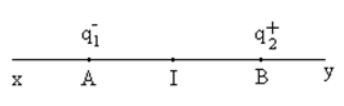
\includegraphics{../figs/VN11-2021-PH-TP004-1}
		\end{center}
	Điểm M mà tại đó cường độ điện trường tổng hợp bằng 0 nằm trên đoạn
		\begin{mcq}(4)
			\item AI.
			\item IB.
			\item B$y$.
			\item A$x$.
		\end{mcq}
		
	}
	\loigiai
	{	\textbf{Đáp án: D.}
		
		Vì $q_1$ và $q_2$ trái dấu nên vị trí cường độ điện trường tổng hợp bằng 0 nằm trên đường thẳng AB và ở phía ngoài đoạn AB.
		
		Vì độ lớn $|q_2| > |q_1|$ nên điểm M nằm gần A hơn.
	}
	\item \mkstar{4}
	
	\cauhoi
	{Một electron chuyển động dọc theo đường sức của một điện trường đều. Cường độ điện trường $E=\SI{100}{V/m}$. Vận tốc ban đầu của electron bằng $\SI{300}{km/s}$. Khối lượng của electron là $m=\SI{9.1e-31}{kg}$. Từ lúc bắt đầu chuyển động đến lúc vận tốc của electron bằng 0 thì electron đã chuyển động được đoạn đường là
		\begin{mcq}(2)
			\item $S=\SI{5.12}{mm}$.
			\item $S=\SI{2.56}{mm}$.
			\item $S=\SI{5.12e-3}{mm}$.
			\item $S=\SI{2.56e-3}{mm}$.
		\end{mcq}
		
	}
	\loigiai
	{	\textbf{Đáp án: B.}
		
		Gia tốc của electron trong điện trường:
		$$a=\dfrac{F}{m} = \dfrac{qE}{m} = \SI{1.76e13}{m/s^2}.$$
		
		Giá trị đại số: $a=\SI{-1.76e13}{m/s^2}$.
		
		Quãng đường chuyển động được:
		$$2aS = v^2 - v_0^2 = 0 - v_0^2 \Rightarrow S \approx \SI{2.56e-3}{m} \approx \SI{2.56}{mm}.$$
	}
\end{enumerate}

\whiteBGstarEnd

\loigiai
{
	\begin{center}
		\textbf{BẢNG ĐÁP ÁN}
	\end{center}
	\begin{center}
		\begin{tabular}{|m{2.8em}|m{2.8em}|m{2.8em}|m{2.8em}|m{2.8em}|m{2.8em}|m{2.8em}|m{2.8em}|m{2.8em}|m{2.8em}|}
			\hline
			1.A  & 2.C  & 3.A  & 4.B  & 5.B  & 6.A  & 7.C  & 8.C  & 9.A  & 10.B  \\
			\hline
			11.B  & 12.B  & 13.A  & 14.D  & 15.B  & 16.B  & 17.A  & 18.C  & 19.D  & 20.B  \\
			\hline
		\end{tabular}
	\end{center}
}
\section{Tự luận}
\begin{enumerate}[label=\bfseries Câu \arabic*:]
	\item \mkstar{1}
	
	\cauhoi{
		Hãy nêu khái niệm, công thức và đặc điểm về phương, chiều, độ lớn của cường độ điện trường.
	}
	
	\loigiai{
		
		Cường độ điện trường là đại lượng vật lý đặc trưng cho tác dụng mạnh hay yếu của điện trường tại một điểm.
		
		Công thức:
		$$\vec E = \dfrac{\vec F}{q}.$$
		
		\begin{itemize}
			\item Điểm đặt: đặt tại điểm đang xét;
			\item Phương: là đường thẳng nối giữa $Q$ và điểm đang xét;
			\item Chiều: hướng ra xa $Q$ nếu $Q$ dương, hướng vào $Q$ nếu $Q$ âm;
			\item Độ lớn: $E=\dfrac{F}{|q|}$, tuy nhiên $E$ không phụ thuộc vào điện tích $q$.
		\end{itemize}
	}
	
	\item \mkstar{2}
	
	\cauhoi{
		Phát biểu nguyên lý chồng chất điện trường. Xác đinh độ lớn của vectơ cường độ điện trường tổng hợp trong các trường hợp sau:
		\begin{enumerate}
			\item $\vec E_1$ cùng phương, cùng chiều với $\vec E_2$;
			\item $\vec E_1$ cùng phương, ngược chiều với $\vec E_2$;
			\item $\vec E_1$ vuông góc với $\vec E_2$;
			\item $\vec E_1$ hợp với $\vec E_2$ một góc $\alpha$ bất kì.
		\end{enumerate}
	}
	
	\loigiai{
		
		Nếu tại một điểm dưới tác dụng của nhiều điện trường $\vec E_1$, $\vec E_2$, $\vec E_3$, $\ldots$ do các điện tích $q_1$, $q_2$, $q_3$, $\ldots$ gây ra thì cường độ điện trường tổng hợp tại đó là
		$$\vec E = \vec E_1 + \vec E_2 + \vec E_3 + \ldots + \vec E_n.$$
		
		Các trường hợp đặc biệt:
		\begin{enumerate}
			\item $\vec E_1$ cùng phương, cùng chiều với $\vec E_2$;
			
			$$E=E_1 + E_2$$
			\item $\vec E_1$ cùng phương, ngược chiều với $\vec E_2$;
			
			$$E=E_1 - E_2$$
			\item $\vec E_1$ vuông góc với $\vec E_2$;
			
			$$E=\sqrt{E_1^2 + E_2^2}$$
			\item $\vec E_1$ hợp với $\vec E_2$ một góc $\alpha$ bất kì.
			
			$$E=\sqrt{E_1^2 + E_2^2 + 2E_1 E_2 \cos \alpha}$$
		\end{enumerate}
		
	}
	\item \mkstar{3}
	
	\cauhoi{
		Một điện tích điểm $q=\SI{e-7}{C}$ đặt tại điểm M trong điện trường do một điện tích điểm $Q$ gây ra và chịu tác dụng của một lực là $F=\SI{3e-3}{N}$.
		\begin{enumerate}
			\item Tính cường độ điện trường do $Q$ gây ra tại điểm M;
			\item Nếu điểm M cách $Q$ một đoạn 30 cm, hãy xác định độ lớn của $Q$.
		\end{enumerate}
	}
	
	\loigiai{
			\begin{enumerate}
			\item Tính cường độ điện trường do $Q$ gây ra tại điểm M;
			$$E_\text{M} = \dfrac{F}{q} = \SI{3e4}{V/m}$$
			\item Nếu điểm M cách $Q$ một đoạn 30 cm, hãy xác định độ lớn của $Q$.
			$$E_\text{M} = k \dfrac{|Q|}{r_\text{M}^2} \Rightarrow |Q|=\dfrac{E_\text{M}r_\text{M}^2}{k} = \SI{3e-7}{C}$$
		\end{enumerate}
		
	}
	\item \mkstar{4}
	
	\cauhoi{
		Tại ba đỉnh của một tam giác ABC vuông tại A, các cạnh $\text{BC} = \SI{50}{cm}$, $\text{AC} = \SI{40}{cm}$, $\text{AB} = \SI{30}{cm}$ ta đặt các điện tích $q_1 = q_2 = q_3 = \SI{e-9}{C}$. Xác định cường độ điện trường tại H với H là chân đường cao kẻ từ A.
	}
	
	\loigiai{
		\begin{center}
			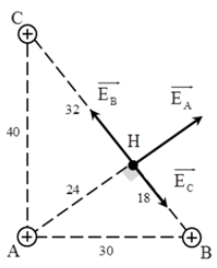
\includegraphics{../figs/VN11-2021-PH-TP004-3}
		\end{center}
	
	Ta có: $\text{HC} = \SI{32}{cm}$, $\text{HB} = \SI{18}{cm}$, $\text{AH} = \SI{24}{cm}$.
	
	Cường độ điện trường gây ra tại H có chiều như hình vẽ trên, về độ lớn:
	$$E_\text{H} = \sqrt{E_\text{A}^2 + (E_\text{B} - E_\text{C})^2} \approx \SI{246}{V/m}.$$
		
	}
	\item \mkstar{4}
	
	\cauhoi{
		Cường độ điện trường của một điện tích phụ thuộc vào khoảng cách $r$ được mô tả như đồ thị dưới đây.
		\begin{center}
			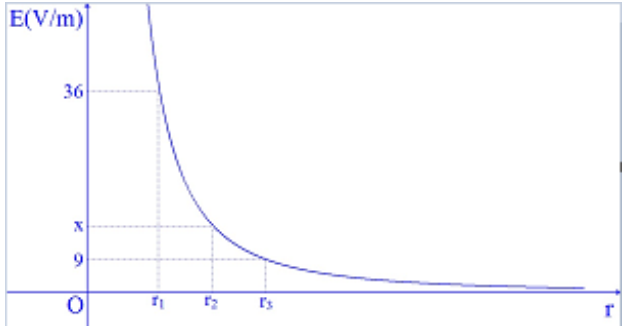
\includegraphics{../figs/VN11-2021-PH-TP004-2}
		\end{center}
	Biết $r_2=\dfrac{r_1+r_3}{2}$ và các điểm cùng nằm trên một đường sức. Tìm giá trị của $x$.
	}
	
	\loigiai{
		
		Ta có $r\sim \dfrac{1}{\sqrt{E}}$, mà $r_2 = \dfrac{r_1+r_3}{2}$ nên suy ra
		$$\dfrac{2}{\sqrt{E_2}} = \dfrac{1}{\sqrt{E_1}} + \dfrac{1}{\sqrt{E_3}} \Rightarrow E_2 = x = \SI{16}{V/m}.$$
	}
	
\end{enumerate}
\stopcontents[mychapters]
%\stopcontents[parts]
%\part[Sóng cơ và sóng âm]{Sóng cơ và sóng âm}
%\startcontents[parts]
%\printcontents[parts]{}{0}{\setcounter{tocdepth}{0}}
\setcounter{mychapter}{3}
\mychapter{Công của lực điện}
\startcontents[mychapters]
\printcontents[mychapters]{}{0}{\setcounter{tocdepth}{1}}
\whiteBGstarBegin
\setcounter{section}{0}
\section{Trắc nghiệm}
\begin{enumerate}[label=\bfseries Câu \arabic*:]
	
	
	\item \mkstar{1}
	
	\cauhoi
	{Công của lực điện trường làm dịch chuyển điện tích $Q$ từ điểm A đến điểm B trong điện trường sẽ phụ thuộc vào
		\begin{mcq}
			\item tọa độ của A và B.
			\item chiều dài quãng đường điện tích di chuyển từ A tới B.
			\item quỹ đạo đi từ A đến B.
			\item khoảng cách AB.
		\end{mcq}
		
	}
	\loigiai
	{	\textbf{Đáp án: A.}
		
		Công của lực điện chỉ phụ thuộc vào tọa độ của điểm đầu và điểm cuối.
	}
	\item \mkstar{1}
	
	\cauhoi
	{Phát biểu nào sau đây về công của lực điện trường là \textbf{không} đúng?
		\begin{mcq}
			\item Khi điện tích chuyển động trên đường thẳng vuông góc với đường sức điện thì công của lực điện trường bằng 0.
			\item Công của lực điện trường phụ thuộc vào hình dạng quỹ đạo chuyển động.
			\item Công của lực điện trường phụ thuộc vào điểm đầu và điểm cuối của quỹ đạo chuyển động.
			\item Công của lực điện trường trên đường cong kín bằng 0.
		\end{mcq}
		
	}
	\loigiai
	{	\textbf{Đáp án: B.}
		
		Công của lực điện trường không phụ thuộc vào hình dạng quỹ đạo chuyển động, mà chỉ phụ thuộc vào điểm đầu và điểm cuối.
	}
	\item \mkstar{2}
	
	\cauhoi
	{Công của lực điện trường dịch chuyển một điện tích $\SI{1}{\micro C}$ dọc theo chiều một đường sức điện trong điện trường đều có độ lớn cường độ điện trường $\SI{1000}{V/m}$ trên quãng đường dài $\SI{1}{m}$ là
		\begin{mcq}(4)
			\item $\SI{1}{mJ}$.
			\item 1 J.
			\item 1000 J.
			\item $\SI{1}{\micro J}$.
		\end{mcq}
		
	}
	\loigiai
	{	\textbf{Đáp án: A.}
		
		Công của lực điện:
		$$A=qEd=\SI{1}{mJ}.$$
	}
	\item \mkstar{2}
	
	\cauhoi
	{Công của lực điện trường khác 0 khi điện tích dịch chuyển như thế nào?
		\begin{mcq}
			\item Dịch chuyển giữa 2 điểm khác nhau cắt các đường sức.
			\item Dịch chuyển vuông góc với các đường sức trong điện trường đều.
			\item Dịch chuyển hết quỹ đạo là đường cong kín trong điện trường.
			\item Dịch chuyển hết một quỹ đạo tròn trong điện trường.
		\end{mcq}
		
	}
	\loigiai
	{	\textbf{Đáp án: A.}
		
		Công của lực điện trường khác 0 khi điện tích dịch chuyển giữa 2 điểm khác nhau cắt các đường sức.
		
		Các trường hợp còn lại đều có $A=0$.
	}
	\item \mkstar{2}
	
	\cauhoi
	{Một điện tích điểm $q$ di chuyển từ điểm M đến điểm N trong điện trường đều như hình vẽ.
		\begin{center}
			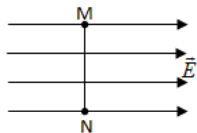
\includegraphics{../figs/VN11-2021-PH-TP005-1}
		\end{center}
	Khẳng định nào sau đây đúng?
		\begin{mcq}
			\item Lực điện trường thực hiện công dương.
			\item Lực điện trường thực hiện công âm.
			\item Lực điện trường không thực hiện công.
			\item Không xác định được công của lực điện trường.
		\end{mcq}
		
	}
	\loigiai
	{	\textbf{Đáp án: C.}
		
		Điện tích dịch chuyển vuông góc với các đường sức nên công của lực điện trường bằng 0.
	}
	\item \mkstar{2}
	
	\cauhoi
	{Khi điện tích dịch chuyển dọc theo một đường sức trong một điện trường đều, nếu quãng đường dịch chuyển tăng 2 lần thì công của lực điện trường
		\begin{mcq}(4)
			\item tăng 4 lần.
			\item tăng 2 lần.
			\item không đổi.
			\item giảm 2 lần.
		\end{mcq}
		
	}
	\loigiai
	{	\textbf{Đáp án: C.}
		
		Công của lực điện trường không phụ thuộc vào quãng đường dịch chuyển của điện tích giữa hai điểm trong điện trường.
	}
	\item \mkstar{2}
	
	\cauhoi
	{Công của lực điện khi di chuyển một điện tích điểm $q=\SI{2e-6}{C}$ qua hiệu điện thế $U=\SI{2}{V}$ có độ lớn là
		\begin{mcq}(4)
			\item $\SI{0.5e-6}{J}$.
			\item $\SI{e-6}{J}$.
			\item $\SI{2e-6}{J}$.
			\item $\SI{4e-6}{J}$.
		\end{mcq}
		
	}
	\loigiai
	{	\textbf{Đáp án: D.}
		
		Áp dụng công thức:
		$$A=qU=\SI{4e-6}{J}.$$
	}
	\item \mkstar{2}
	
	\cauhoi
	{Xác định công của lực điện trường khi di chuyển một electron từ điểm A đến điểm B. Biết hiệu điện thế giữa hai điểm A và B là $U=\SI{5}{V}$.
		\begin{mcq}(4)
			\item $A=\SI{-5}{eV}$.
			\item $A=\SI{5}{eV}$.
			\item $A=\SI{8e-18}{J}$.
			\item $A=\SI{-8e-18}{J}$.
		\end{mcq}
		
	}
	\loigiai
	{	\textbf{Đáp án: A.}
		
		Áp dụng công thức:
		$$A=qU=eU=e\cdot \SI{5}{V} = \SI{5}{eV}.$$
		
		Vì $U_\text{AB} > 0$ nên điện thế tại A cao hơn điện thế tại B, suy ra công của lực điện trường tác dụng lên electron khi nó dịch chuyển từ A đến B là công cản, vậy $A=\SI{-5}{eV}$.
	}
	\item \mkstar{2}
	
	\cauhoi
	{Một điện tích điểm $q$ chuyển động trong điện trường đều $E$ có quỹ đạo là một đường cong khép kín. Gọi chiều dài quỹ đạo là $s$ thì công của lực điện trường là
		\begin{mcq}(4)
			\item $A=2qEs$.
			\item $A=0$.
			\item $A=qEs$.
			\item $A=qE/s$.
		\end{mcq}
		
	}
	\loigiai
	{	\textbf{Đáp án: B.}
		
		Công của lực điện trường làm dịch chuyển một điện tích theo một đường cong khép kín bằng 0.
	}
	\item \mkstar{2}
	
	\cauhoi
	{Công của lực điện trường làm dịch chuyển một điện tích $\SI{-2}{\micro C}$ ngược chiều một đường sức trong điện trường đều có độ lớn $\SI{1000}{V/m}$ trên quãng đường dài $\SI{1}{m}$. Xác định công của lực điện trường trong trường hợp này.
		\begin{mcq}(4)
			\item $A=\SI{2000}{J}$.
			\item $A=\SI{-2000}{J}$.
			\item $A=\SI{2}{mJ}$.
			\item $A=\SI{-2}{mJ}$.
		\end{mcq}
		
	}
	\loigiai
	{	\textbf{Đáp án: C.}
		
		Vì điện tích $q<0$ nên khi dịch chuyển ngược chiều điện trường, công của lực điện tác dụng lên điện tích là công phát động ($A>0$).
		
		Áp dụng công thức:
		$$A=qEd  =\SI{2}{mJ}.$$
	}
	\item \mkstar{2}
	
	\cauhoi
	{Một electron di chuyển được một đoạn đường $\SI{1}{cm}$ dọc theo đường sức điện trong một điện trường đều có cường độ $\SI{1000}{V/m}$. Xác định công của lực điện trong dịch chuyển trên.
		\begin{mcq}(4)
			\item $\SI{-1.6e-18}{J}$.
			\item $\SI{1.6e-16}{J}$.
			\item $\SI{1.6e-18}{J}$.
			\item $\SI{-1.6e-16}{J}$.
		\end{mcq}
		
	}
	\loigiai
	{	\textbf{Đáp án: C.}
		
		Vì lực điện tác dụng lên electron cùng chiều với chiều dịch chuyển của electron nên sinh công dương.
		
		Áp dụng công thức:
		$$A=qEd=eEd = \SI{1.6e-18}{J}.$$
	}
	\item \mkstar{2}
	
	\cauhoi
	{Trong một điện trường đều cường độ $\SI{60000}{V/m}$ có điện tích $q_0=\SI{4e-9}{C}$ dịch chuyển trên đoạn thẳng dài $\SI{5}{cm}$. Biết góc giữa phương dịch chuyển và đường sức điện là $\alpha = 60^\circ$. Xác định công của lực điện trong trường hợp trên.
		\begin{mcq}(4)
			\item $\SI{e-6}{J}$.
			\item $\SI{6e6}{J}$.
			\item $\SI{6e-6}{J}$.
			\item $\SI{-6e-6}{J}$.
		\end{mcq}
		
	}
	\loigiai
	{	\textbf{Đáp án: C.}
		
		Áp dụng công thức:
		$$A=qEd=qEs \cos \alpha = \SI{6e-6}{J}.$$
	}
	\item \mkstar{2}
	
	\cauhoi
	{Công của lực điện trường làm dịch chuyển một điện tích $q>0$ một đoạn $d$ theo hướng của một đường sức điện trong điện trường đều có cường độ $E$ có biểu thức
		\begin{mcq}(4)
			\item $A=\dfrac{qE}{d}$.
			\item $A=qEd$.
			\item $A=-\dfrac{qE}{d}$.
			\item $A=-qEd$.
		\end{mcq}
		
	}
	\loigiai
	{	\textbf{Đáp án: B.}
		
		Vì điện tích dịch chuyển cùng chiều với lực điện nên công dương: $A=qEd$.
	}
	\item \mkstar{2}
	
	\cauhoi
	{Cho điện tích $q$ dịch chuyển giữa hai điểm cố định trong một điện trường đều có cường độ $\SI{150}{V/m}$ thì công của lực điện trường là $\SI{60}{mJ}$. Nếu cường độ điện trường là $\SI{200}{V/m}$ thì công của lực điện trường tương ứng là
		\begin{mcq}(4)
			\item $\SI{40}{J}$.
			\item $\SI{40}{mJ}$.
			\item $\SI{80}{J}$.
			\item $\SI{80}{mJ}$.
		\end{mcq}
		
	}
	\loigiai
	{	\textbf{Đáp án: D.}
		
		Lập tỉ lệ:
		$$\dfrac{A_1}{A_2} = \dfrac{E_1}{E_2} = \dfrac{3}{4} \Rightarrow A_2 = \SI{80}{mJ}.$$
	}
	\item \mkstar{2}
	
	\cauhoi
	{Khi điện tích dịch chuyển trong điện trường đều dọc theo chiều đường sức thì công của lực điện tác dụng lên nó là $\SI{10}{J}$. Cũng với điện tích ấy và khoảng cách dịch chuyển ấy, nếu chiều dịch chuyển hợp với chiều đường sức một góc $60^\circ$ thì công của lực điện là
		\begin{mcq}(4)
			\item $\SI{7.5}{J}$.
			\item $\xsi{\dfrac{5\sqrt{3}}{2}}{J}$.
			\item $\SI{5}{J}$.
			\item $\xsi{5\sqrt{2}}{J}$.
		\end{mcq}
		
	}
	\loigiai
	{	\textbf{Đáp án: C.}
		
		Lập tỉ lệ:
		$$\dfrac{A_1}{A_2} = \dfrac{\cos 0}{\cos 60^\circ} = 2 \Rightarrow A_2 = \SI{5}{J}.$$
	}
	\item \mkstar{3}
	
	\cauhoi
	{Dưới tác dụng của lực điện trường, một điện tích $q$ dương di chuyển được một đoạn đường $s$ trong điện trường đều theo phương hợp với $\vec E$ một góc $\alpha$. Trong trường hợp nào sau đây, công của lực điện trường là lớn nhất?
		\begin{mcq}(4)
			\item $\alpha = 0^\circ$.
			\item $\alpha=45^\circ$.
			\item $\alpha = 60^\circ$.
			\item $\alpha=90^\circ$.
		\end{mcq}
		
	}
	\loigiai
	{	\textbf{Đáp án: A.}
		
		Khi $\alpha = 0$ thì điện tích dịch chuyển theo phương đường sức, khi đó công của lực điện trường là lớn nhất.
	}
	\item \mkstar{3}
	
	\cauhoi
	{Cho điện tích thử $q$ di chuyển trong một điện trường đều dọc theo hai đoạn thẳng MN và NP. Biết rằng lực điện sinh công dương và MN dài hơn NP. Hỏi biểu thức nào sau đây là đúng?
		\begin{mcq}(2)
			\item $A_\text{MN} > A_\text{NP}$.
			\item $A_\text{MN} < A_\text{NP}$.
			\item $A_\text{MN} = A_\text{NP}$.
			\item Cả 3 biểu thức đều đúng.
		\end{mcq}
		
	}
	\loigiai
	{	\textbf{Đáp án: D.}
		
		Tùy thuộc vào góc $\alpha$ mà độ lớn công của lực điện khác nhau. Do đó cả 3 trường hợp đều có thể xảy ra.
	}
	\item \mkstar{3}
	
	\cauhoi
	{Công của lực điện trường dịch chuyển một điện tích điểm $q=\SI{5}{\micro C}$ đi từ điểm M đến điểm N ($\text{MN} = \SI{2}{cm}$) trong một điện trường đều có cường độ $E=\SI{e5}{V/m}$ là bao nhiêu? Biết $\overrightarrow{\text{MN}}$ vuông góc $\vec E$.
		\begin{mcq}(4)
			\item 1 J.
			\item 1000 J.
			\item 100 mJ.
			\item 0 J.
		\end{mcq}
		
	}
	\loigiai
	{	\textbf{Đáp án: D.}
		
		Do $\overrightarrow{\text{MN}}\ \bot \vec{E}$ nên $A=0$.
	}
	\item \mkstar{3}

	\cauhoi
	{Một ion hidro $\ce{H}^+$ được đặt vào trong một điện trường đều với cường độ điện trường $E=\SI{e4}{V/m}$. Khi ion hidro này dịch chuyển được $\SI{0.1}{mm}$ thì đã nhận được công của lực điện với giá trị là
		\begin{mcq}(4)
			\item $\SI{0}{J}$.
			\item $\SI{-1.6e-19}{J}$.
			\item $\SI{e-19}{J}$.
			\item $\SI{1.6e-19}{J}$.
		\end{mcq}
		
	}
	\loigiai
	{	\textbf{Đáp án: D.}
		
		Ion $\ce{H}^+$ có điện tích $q=+\SI{1.6e-19}{C}$.
		
		Đổi $d=\SI{0.1}{mm}=\SI{1e-4}{m}$
		
		Áp dụng công thức:
		$$A=qEd = \SI{1.6e-19}{J}.$$
	}
	\item \mkstar{4}
	
	\cauhoi
	{Một điện tích $q=\SI{4e-8}{C}$ di chuyển trong một điện trường đều có cường độ $E=\SI{100}{V/m}$ theo một đường gấp khúc ABC. Đoạn AB dài 20 cm và vectơ độ dời $\overrightarrow{\text{AB}}$ làm với các đường sức điện một góc $30^\circ$. Đoạn BC dài 40 cm và vectơ độ dời $\overrightarrow{\text{BC}}$ làm với các đường sức điện một góc $120^\circ$. Tính công của lực điện khi điện tích di chuyển từ A đến C.
		\begin{mcq}(4)
			\item $\SI{1.5e-6}{J}$.
			\item $\SI{-1.5e-6}{J}$.
			\item $\SI{0.1e-6}{J}$.
			\item $\SI{-0.1e-6}{J}$.
		\end{mcq}
		
	}
	\loigiai
	{	\textbf{Đáp án: D.}
		
		\begin{center}
			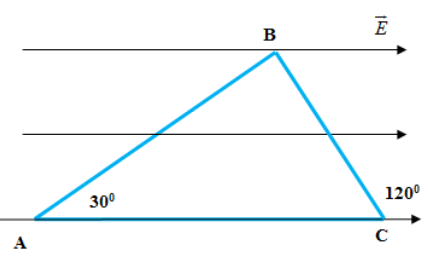
\includegraphics{../figs/VN11-2021-PH-TP005-2}
		\end{center}
	
	Công của lực điện trên đoạn AB:
	$$A_\text{AB} = qE \cdot \text{AB} \cdot \cos 30^\circ = \SI{0.7e-6}{J}.$$
	
	Công của lực điện trên đoạn BC:
	$$A_\text{BC} = qE \cdot\ \text{BC} \cdot \cos 120^\circ = \SI{-0.8e-6}{J}.$$
	
	Công của lực điện trên đoạn ABC:
	$$A_\text{ABC} = A_\text{AB} + A_\text{BC} = \SI{-0.1e-6}{J}.$$
	}
\end{enumerate}

\whiteBGstarEnd

\loigiai
{
	\begin{center}
		\textbf{BẢNG ĐÁP ÁN}
	\end{center}
	\begin{center}
		\begin{tabular}{|m{2.8em}|m{2.8em}|m{2.8em}|m{2.8em}|m{2.8em}|m{2.8em}|m{2.8em}|m{2.8em}|m{2.8em}|m{2.8em}|}
			\hline
			1.A  & 2.B  & 3.A  & 4.A  & 5.C  & 6.C  & 7.D  & 8.A  & 9.B  & 10.C  \\
			\hline
			11.C  & 12.C  & 13.B  & 14.D  & 15.C  & 16.A  & 17.D  & 18.D  & 19.D  & 20.D  \\
			\hline
		\end{tabular}
	\end{center}
}
\section{Tự luận}
\begin{enumerate}[label=\bfseries Câu \arabic*:]
	\item \mkstar{1}
	
	\cauhoi{
		Nêu đặc điểm, biểu thức, giải thích các đại lượng trong biểu thức tính công của lực điện.
	}
	
	\loigiai{
		
		Đặc điểm: Công của lực điện tác dụng lên một điện tích không phụ thuộc vào hình dạng quỹ đạo mà chỉ phụ thuộc vào vị trí của điểm đầu và điểm cuối của quỹ đạo.
		
		Biểu thức: $A=qEd$, trong đó:
		\begin{itemize}
			\item $d$ là hình chiếu của quỹ đạo lên phương đường sức điện (m);
			\item $E$ là cường độ điện trường (V/m);
			\item $q$ là điện tích (C).
		\end{itemize}
		
	}
	
	\item \mkstar{2}
	
	\cauhoi{
		Một electron di chuyển một đoạn $\SI{0.6}{cm}$ từ điểm M đến điểm N dọc theo một đường sức điện của một điện trường đều thì lực điện sinh công $\SI{9.6e-18}{J}$. Tính độ lớn của cường độ điện trường $E$.
	}
	
	\loigiai{
		
		Áp dụng công thức:
		$$A=qEd \Rightarrow E = \dfrac{A}{qd} = \SI{e4}{V/m}.$$
	}
	\item \mkstar{3}
	
	\cauhoi{
		Một electron bay dọc theo hướng đường sức của điện trường đều với vận tốc tại A là $\SI{5e6}{m/s}$, sau đó dừng lại tại B với $\text{AB} = d = \SI{10}{cm}$. Tính độ lớn của cường độ điện trường.
	}
	
	\loigiai{
		
	Áp dụng định lý động năng, ta có:
	$$0-\dfrac{1}{2}mv_\text{A}^2 = qEd \Rightarrow E=\SI{710.94}{V/m}.$$	
	}
	\item \mkstar{4}
	
	\cauhoi{
		Hai tấm kim loại đặt song song, cách nhau 2 cm, được nhiễm điện trái dấu nhau và có độ lớn bằng nhau. Muốn điện tích $q=\SI{5e-10}{C}$ di chuyển từ tấm này đến tấm kia cần tốn một công $A=\SI{2e-9}{J}$. Hãy xác định cường độ điện trường bên trong hai tấm kim loại đó, biết rằng điện trường bên trong hai tấm là điện trường đều và có các đường sức vuông góc với hai tấm.
	}
	
	\loigiai{
		
		Cường độ điện trường bên trong hai tấm:
		$$E=\dfrac{A}{qd} = \SI{200}{V/m}.$$
	}
	\item \mkstar{4}
	
	\cauhoi{
		Lực điện trường sinh công $\SI{9.6e-18}{J}$ dịch chuyển một electron (đang đứng yên) dọc theo đường sức được một quãng đường $\SI{0.6}{cm}$. Nếu đi thêm một đoạn $\SI{0.4}{cm}$ nữa theo chiều như cũ thì vận tốc của electron ở cuối đoạn đường là bao nhiêu?
	}
	
	\loigiai{
		
	Ta có: $A_1 = \SI{9.6e-18}{J}$, $s_1=\SI{0.6}{cm}$, $s_2=\SI{1}{cm}$, $v_0=0$.
	
	Lực điện sinh công dương nên elelctron chuyển động ngược chiều điện trường.
	
	Công lúc đầu:
	$$A_1=-qEs_1 \Rightarrow E = \SI{e4}{V/m}.$$
	
	Công lúc sau (dương):
	$$A_2=qEs_2=\SI{1.6e-17}{J}.$$
	
	Áp dụng định lý động năng:
	$$A_2=\dfrac{1}{2}mv_2^2 - A_1 \Rightarrow v_2=\SI{75e5}{m/s}.$$	
	}
	
\end{enumerate}
\stopcontents[mychapters]
\setcounter{mychapter}{4}
\mychapter{Điện thế. Hiệu điện thế}
\startcontents[mychapters]
\printcontents[mychapters]{}{0}{\setcounter{tocdepth}{1}}
\whiteBGstarBegin
\setcounter{section}{0}
\section{Trắc nghiệm}
\begin{enumerate}[label=\bfseries Câu \arabic*:]
	
	
	\item \mkstar{1}
	
	\cauhoi
	{Điều nào sau đây \textbf{không đúng} khi nói về quan hệ giữa cường độ điện trường và hiệu điện thế?
		\begin{mcq}
			\item Vectơ cường độ điện trường hướng từ nơi có điện thế cao về nơi có điện thế thấp.
			\item Trong một điện trường đều, hiệu điện thế giữa hai điểm này và giữa hai điểm khác có thể bằng nhau.
			\item Hiệu điện thế giữa hai điểm trên cùng một đường sức trong một điện trường đều có thể bằng 0.
			\item Cường độ điện trường tỉ lệ thuận với hiệu điện thế.
		\end{mcq}
		
	}
	\loigiai
	{	\textbf{Đáp án: C.}
	
	}
	\item \mkstar{1}
	
	\cauhoi
	{Cho một điện trường đều có cường độ $E$. Chọn chiều dương cùng chiều với đường sức điện. Gọi $U$ là hiệu điện thế giữa hai điểm M và N trên cùng một đường sức, $d=\overline{\text{MN}}$ là độ dài đại số đoạn MN. Hệ thức nào sau đây đúng?
		\begin{mcq}(4)
			\item $E=\dfrac{U}{2d}$.
			\item $E=\dfrac{U}{d}$.
			\item $E=Ud$.
			\item $E=2Ud$.
		\end{mcq}
		
	}
	\loigiai
	{	\textbf{Đáp án: B.}
	
	}
	\item \mkstar{1}
	
	\cauhoi
	{Trên một đường sức của điện trường đều có hai điểm M và N cách nhau 40 cm. Hiệu điện thế giữa hai điểm M và N là 16 V. Cường độ điện trường có độ lớn là
		\begin{mcq}(4)
			\item 4000 V/m.
			\item 40 V/m.
			\item 400 V/m.
			\item 4 V/m.
		\end{mcq}
		
	}
	\loigiai
	{	\textbf{Đáp án: B.}
		
		Áp dụng công thức:
		$$E=\dfrac{U}{d} = \SI{40}{V/m}.$$
	}
	\item \mkstar{2}
	
	\cauhoi
	{Công của lực điện trường dịch chuyển một điện tích $\SI{-2}{\micro C}$ từ A đến B là 4 mJ. Hiệu điện thế giữa hai điểm A và B là
		\begin{mcq}(4)
			\item 2 V.
			\item 2000 V.
			\item -8 V.
			\item -2000 V.
		\end{mcq}
		
	}
	\loigiai
	{	\textbf{Đáp án: D.}
		
		Áp dụng công thức:
		$$A=qU \Rightarrow U = \SI{-2000}{V}.$$
	}
	\item \mkstar{2}
	
	\cauhoi
	{Hai điểm M và N cùng nằm trên một đường sức của một điện trường đều cách nhau $\SI{2}{m}$. Độ lớn của cường độ điện trường là 500 V/m. Hiệu điện thế giữa hai điểm đó là
		\begin{mcq}(4)
			\item 1000 V.
			\item 125 V.
			\item 2000 V.
			\item 0 V.
		\end{mcq}
		
	}
	\loigiai
	{	\textbf{Đáp án: A.}
		
		Áp dụng công thức:
	$$U=Ed \Rightarrow U = \SI{1000}{V}.$$
	}
	\item \mkstar{2}
	
	\cauhoi
	{Hiệu điện thế giữa hai điểm M và N là $U_\text{MN} = \SI{1}{V}$. Công của lực điện trường làm dịch chuyển điện tích $q=\SI{-1}{\micro C}$ từ M đến N là
		\begin{mcq}(4)
			\item $\SI{-1}{\micro J}$.
			\item $\SI{1}{\micro J}$.
			\item $\SI{-1}{J}$.
			\item $\SI{1}{J}$.
		\end{mcq}
		
	}
	\loigiai
	{	\textbf{Đáp án: A.}
		
		Vì $U_\text{MN} = \SI{1}{V} >0$ nên công của lực điện trường làm dịch chuyển điện tích âm từ M đến N là công cản.
		
		Áp dụng công thức: $A=qU = \SI{-1}{\micro J}$.
	}
	\item \mkstar{2}
	
	\cauhoi
	{Thế năng tĩnh điện của một electron tại điểm M trong điện trường của một điện tích điểm là $\SI{-3.2e-19}{J}$. Điện thế tại điểm M là
		\begin{mcq}(4)
			\item $\SI{3.2}{V}$.
			\item $\SI{-3.2}{V}$.
			\item $\SI{2}{V}$.
			\item $\SI{-2}{V}$.
		\end{mcq}
		
	}
	\loigiai
	{	\textbf{Đáp án: C.}
		
		Áp dụng công thức:
		$$V_\text{M} = \dfrac{A_\text{M}}{q} = \SI{2}{V}.$$
	}
	\item \mkstar{2}
	
	\cauhoi
	{Khi độ lớn điện tích thử đặt tại một điểm tăng lên gấp đôi thì điện thế tại điểm đó
		\begin{mcq}(2)
			\item không đổi.
			\item tăng gấp đôi.
			\item giảm một nửa.
			\item tăng gấp bốn.
		\end{mcq}
		
	}
	\loigiai
	{	\textbf{Đáp án: A.}
		
		Điện thế tại một điểm không phụ thuộc vào độ lớn điện tích thử.
	}
	\item \mkstar{2}
	
	\cauhoi
	{Biết hiệu điện thế giữa hai điểm M, N là $U_\text{MN}=\SI{7}{V}$. Gọi $V_\text{M}$, $V_\text{N}$ lần lượt là điện thế tại M và N. Khẳng định nào sau đây đúng nhất?
		\begin{mcq}(2)
			\item $V_\text{M} = V_\text{N} = \SI{7}{V}$.
			\item $V_\text{M} - V_\text{N} = \SI{7}{V}$.
			\item $V_\text{N} - V_\text{M} = \SI{7}{V}$.
			\item $V_\text{N} + V_\text{M} = \SI{7}{V}$.
		\end{mcq}
		
	}
	\loigiai
	{	\textbf{Đáp án: B.}
		
		Nếu $U_\text{MN} = \SI{7}{V}$ thì có nghĩa là $V_\text{M} - V_\text{N} = \SI{7}{V}$.
	}
	\item \mkstar{2}
	
	\cauhoi
	{Hiệu điện thế giữa hai điểm M, N là 40 V. Chọn câu đúng nhất.
		\begin{mcq}
			\item Điện thế tại M là 40 V, điện thế tại N là 0 V.
			\item Điện thế tại M cao hơn điện thế tại N là 40 V.
			\item Điện thế tại M có giá trị dương, điện thế tại N có giá trị âm.
			\item Điện thế tại N là 40 V, điện thế tại M là 0 V.
		\end{mcq}
		
	}
	\loigiai
	{	\textbf{Đáp án: B.}
		
		Hiệu điện thế giữa hai điểm M, N là $\SI{40}{V}$ thì điện thế tại M cao hơn điện thế tại N là $\SI{40}{V}$.
	}
	\item \mkstar{2}
	
	\cauhoi
	{Mối liên hệ giữa $U_\text{MN}$ và $U_\text{NM}$ là
		\begin{mcq}(4)
			\item $U_\text{MN} = U_\text{NM}$.
			\item $U_\text{MN} = - U_\text{NM}$.
			\item $U_\text{MN} = \dfrac{1}{U_\text{NM}}$.
			\item $U_\text{MN} = -\dfrac{1}{U_\text{NM}}$.
		\end{mcq}
		
	}
	\loigiai
	{	\textbf{Đáp án: B.}
	
	}
	\item \mkstar{2}
	
	\cauhoi
	{Trên một đường sức của một điện trường đều có hai điểm M và N cách nhau 40 cm. Hiệu điện thế giữa hai điểm M và N là 80 V. Cường độ điện trường có độ lớn là
		\begin{mcq}(4)
			\item 2000 V/m.
			\item 2 V/m.
			\item 200 V/m.
			\item 20 V/m.
		\end{mcq}
		
	}
	\loigiai
	{	\textbf{Đáp án: C.}
		
		Áp dụng công thức:
		$$E=\dfrac{U}{d} \Rightarrow E = \SI{200}{V/m}.$$
	}
	\item \mkstar{2}
	
	\cauhoi
	{Giữa hai điểm A và B phải có hiệu điện thế bằng bao nhiêu để một điện tích $q=\SI{1}{\micro C}$ thu được năng lượng $A=\SI{2e-4}{J}$ khi đi giữa hai điểm đó?
		\begin{mcq}(4)
			\item 100 V.
			\item 200 V.
			\item 300 V.
			\item 500 V.
		\end{mcq}
		
	}
	\loigiai
	{	\textbf{Đáp án: B.}
		
		Áp dụng công thức:
		$$A=qU \Rightarrow U = \SI{200}{V}.$$
	}
	\item \mkstar{2}
	
	\cauhoi
	{Hiệu điện thế giữa hai điểm M và N trong một điện trường đều là $U_\text{MN} = \SI{20}{V}$. Một điện tích dịch chuyển cùng chiều điện trường từ M đến N dưới tác dụng của lực điện, với công của lực điện bằng $\SI{1.6e-10}{J}$. Giá trị của điện tích này là
		\begin{mcq}(4)
			\item $q=\SI{6e-6}{C}$.
			\item $q=\SI{6e-9}{C}$.
			\item $q=\SI{8e-12}{C}$.
			\item $q=\SI{8e-15}{C}$.
		\end{mcq}
		
	}
	\loigiai
	{	\textbf{Đáp án: C.}
		
		Áp dụng công thức:
	$$A=qU \Rightarrow q = \SI{8e-12}{C}.$$
	}
	\item \mkstar{2}
	
	\cauhoi
	{Tính công mà lực điện tác dụng lên một electron khi nó chuyển động từ điểm M đến điểm N. Biết hiệu điện thế $U_\text{MN} = \SI{50}{V}$.
		\begin{mcq}(4)
			\item $\SI{8e-18}{J}$.
			\item $\SI{-8e-18}{J}$.
			\item $\SI{3.2e-21}{J}$.
			\item $\SI{-3.2e-21}{J}$.
		\end{mcq}
		
	}
	\loigiai
	{	\textbf{Đáp án: B.}
		
		Áp dụng công thức:
		$$A=qU=\SI{8e-18}{J}.$$
		
		Mà công làm dịch chuyển electron từ M đến N là công âm, nên $A=\SI{-8e-18}{J}$.
	}
	\item \mkstar{3}
	
	\cauhoi
	{Cho 3 điểm M, N, P trong một điện trường đều. Cho $\text{MN} = \SI{3}{cm}$, $\text{NP} = \SI{1}{cm}$, $U_\text{MN} = \SI{3}{V}$, $U_\text{MP} = \SI{1}{V}$. Gọi cường độ điện trường tại M, N, P lần lượt là $E_\text{M}$, $E_\text{N}$, $E_\text{P}$. Kết luận đúng là
		\begin{mcq}(4)
			\item $E_\text{N} > E_\text{M}$.
			\item $E_\text{P} = 2E_\text{N}$.
			\item $E_\text{P} = 3E_\text{N}$.
			\item $E_\text{P} = E_\text{N}$.
		\end{mcq}
		
	}
	\loigiai
	{	\textbf{Đáp án: D.}
		
		Trong một điện trường đều, cường độ điện trường tại mọi điểm bằng nhau.
	}
	\item \mkstar{3}
	
	\cauhoi
	{Trong một điện trường đều, nếu trên một đường sức, giữa hai điểm cách nhau 4 cm có hiệu điện thế 10 V, thì giữa hai điểm cách nhau 6 cm sẽ có hiệu điện thế là
		\begin{mcq}(4)
			\item 8 V.
			\item 10 V.
			\item 15 V.
			\item $\SI{22.5}{V}$.
		\end{mcq}
		
	}
	\loigiai
	{	\textbf{Đáp án: C.}
		
		Ta có:
		$$E=\dfrac{U_1}{d_1} = \dfrac{U_2}{d_2} \Rightarrow U_2 = \dfrac{U_1 d_2}{d_1} = \SI{15}{V}.$$
	}
	\item \mkstar{3}
	
	\cauhoi
	{Một proton bay vào trong điện trường. Lúc proton ở điểm A thì tốc độ của nó là $\SI{2.5e4}{m/s}$. Khi bay đến B tốc độ của proton bằng 0. Điện thế tại A bằng $\SI{500}{V}$, điện thế tại B gần giá trị nào nhất sau đây? Cho biết proton có khối lượng $\SI{1.67e-27}{kg}$ và có điện tích $\SI{1.6e-19}{C}$.
		\begin{mcq}(4)
			\item $\SI{403.3}{V}$.
			\item $\SI{503.3}{V}$.
			\item $\SI{703.3}{V}$.
			\item $\SI{603.3}{V}$.
		\end{mcq}
		
	}
	\loigiai
	{	\textbf{Đáp án: B.}
		
		Áp dụng định lý động năng cho chuyển động của proton từ điểm A đến điểm B:
		$$W_\text{đ B} - W_\text{đ A} = qU_\text{AB} \Rightarrow U_\text{AB} = \SI{-3.26}{V}.$$
		
		Mà $U_\text{AB} = V_\text{A} - V_\text{B} \Rightarrow V_\text{B} \approx \SI{503.3}{V}$.
	}
	\item \mkstar{3}
	
	\cauhoi
	{Một electron bay với vận tốc $\SI{1.2e7}{m/s}$ từ một điểm có điện thế $V_1=\SI{600}{V}$ dọc theo hướng các đường sức của một điện trường đều. Biết điện tích của electron là $\SI{-1.6e-19}{C}$ và khối lượng của nó là $\SI{9.1e-31}{kg}$. Điện thế $V_2$ tại điểm mà ở đó electron dừng lại là
		\begin{mcq}(4)
			\item $\SI{150.4}{V}$.
			\item $\SI{170.5}{V}$.
			\item $\SI{190.5}{V}$.
			\item $\SI{200}{V}$.
		\end{mcq}
		
	}
	\loigiai
	{	\textbf{Đáp án: C.}
		
		Áp dụng định lý động năng:
		$$W_\text{đ 2} - W_\text{đ 1} = A \Leftrightarrow -\dfrac{mv^2}{2} = q(V_1 - V_2) \Rightarrow V_2 = \SI{190.5}{V}.$$
	}
	\item \mkstar{4}
	
	\cauhoi
	{Cho ba bản kim loại phẳng tích điện 1, 2, 3 đặt song song lần lượt cách nhau những khoảng $d_{12} = \SI{5}{cm}$, $d_{23} = \SI{8}{cm}$. Bản 1 và 3 tích điện dương, bản 2 tích điện âm. Biết $E_{12}=\SI{4e4}{V/m}$, $E_{23} = \SI{5e4}{V/m}$. Tính điện thế $V_2$, $V_3$ của các bản 2 và 3 nếu lấy gốc điện thế ở bản 1 ($V_1=0$).
		\begin{mcq}(2)
			\item $V_2=\SI{2000}{V}$, $V_3=\SI{-2000}{V}$.
			\item $V_2\SI{2000}{V}$, $V_3=\SI{4000}{V}$.
			\item $V_2=\SI{-2000}{V}$, $V_3=\SI{4000}{V}$.
			\item $V_2=\SI{-2000}{V}$, $V_3=\SI{2000}{V}$.
		\end{mcq}
		
	}
	\loigiai
	{	\textbf{Đáp án: D.}
		
		Ta có:
		$$U_{12} = E_{12} d_{12} = \SI{2000}{V};$$
		$$U_{32} = E_{32} d_{32} = \SI{4000}{V}.$$
		
		Vì bản 1 và 3 tích điện dương, bản 2 tích điện âm nên khi chọn $V_1=0$ thì
		$$U_{12} = V_1 - V_2 \Rightarrow V_2 = \SI{-2000}{V}.$$
		$$U_{32} = V_3 - V_2 \Rightarrow V_3 = \SI{2000}{V}.$$
	}
\end{enumerate}

\whiteBGstarEnd

\loigiai
{
	\begin{center}
		\textbf{BẢNG ĐÁP ÁN}
	\end{center}
	\begin{center}
		\begin{tabular}{|m{2.8em}|m{2.8em}|m{2.8em}|m{2.8em}|m{2.8em}|m{2.8em}|m{2.8em}|m{2.8em}|m{2.8em}|m{2.8em}|}
			\hline
			1.C  & 2.B  & 3.B  & 4.D  & 5.A  & 6.A  & 7.C  & 8.A  & 9.B  & 10.B  \\
			\hline
			11.B  & 12.C  & 13.B  & 14.C  & 15.B  & 16.D  & 17.C  & 18.B  & 19.C  & 20.D  \\
			\hline
		\end{tabular}
	\end{center}
}
\section{Tự luận}
\begin{enumerate}[label=\bfseries Câu \arabic*:]
	\item \mkstar{1}
	
	\cauhoi{
		Điện thế tại một điểm là gì? Hiệu điện thế giữa hai điểm trong điện trường là gì? Nêu công thức định nghĩa hai đại lượng trên.
	}
	
	\loigiai{
		
		Điện thế tại một điểm M trong điện trường là đại lượng đặc trưng cho điện trường về phương diện tạo ra thế năng khi đặt tại đó một điện tích $q$.
		
		Công thức:
		$$V_\text{M} = \dfrac{A}{Q}.$$
		
		Hiệu điện thế giữa hai điểm trong điện trường là đại lượng đặc trưng cho khả năng thực hiện công của điện trường khi có 1 điện tích di chuyển giữa hai điểm đó.
		
		Công thức:
		$$U_\text{MN} = V_\text{M} - V_\text{N} = \dfrac{A_\text{MN}}{q}.$$
	}
	
	\item \mkstar{2}
	
	\cauhoi{
		Khi bay từ điểm M đến điểm N trong điện trường, electron tăng tốc, động năng tăng thêm $\SI{250}{eV}$. Biết rằng $\SI{1}{eV} = \SI{1.6e-19}{J}$, xác định $U_\text{MN}$.
	}
	
	\loigiai{
		Áp dụng định lý động năng:
		$$A=W_\text{đ 2} - W_\text{đ 1} = \SI{4e-17}{J}.$$
		
		Hiệu điện thế:
		$$U_\text{MN} = \dfrac{A}{q} = \SI{-250}{V}.$$
		
	}
	\item \mkstar{3}
	
	\cauhoi{
		Bắn một electron (tích điện $-|e|$ và khối lượng $m$) với vận tốc $v_0$ vào điện trường đều giữa hai bản kim loại phẳng theo phương song song, cách đều hai bản kim loại (xem hình vẽ).
		\begin{center}
			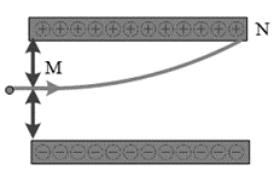
\includegraphics{../figs/VN11-2021-PH-TP006-1}
		\end{center}
	
	Hiệu điện thế giữa hai bản là 200 V. Biết rằng electron bay ra khỏi điện trường tại điểm nằm sát mép một bản. Công của lực điện trong sự dịch chuyển của electron trong điện trường là bao nhiêu?
	}
	
	\loigiai{
	Công của lực điện:
	$$A_\text{MN} = qU_\text{MN} = -|e| \dfrac{-U}{2} = \SI{0.5}{} |e| U = \SI{1.6e-17}{J}.$$	
		
	}
	\item \mkstar{4}
	
	\cauhoi{
		Một quả cầu khối lượng $\SI{4.5e-3}{kg}$ treo vào một sợi dây cách điện dài 1 m. Quả cầu nằm giữa hai tấm kim loại song song, thẳng đứng như hình vẽ.
		\begin{center}
			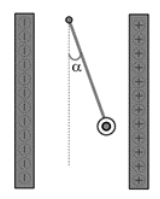
\includegraphics{../figs/VN11-2021-PH-TP006-2}
		\end{center}
	
	Hai tấm cách nhau 4 cm. Đặt một hiệu điện thế 75 V vào hai tấm đó thì quả cầu lệch ra khỏi vị trí ban đầu 1 cm. Lấy $g=\SI{10}{m/s^2}$. Tính độ lớn điện tích của quả cầu.
	}
	
	\loigiai{
		\begin{center}
			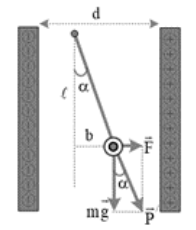
\includegraphics{../figs/VN11-2021-PH-TP006-4}
		\end{center}
		
		Quả cầu lệch về bản dương nên nó tích điện âm. Khi hệ cân bằng thì
		$$\tan \alpha = \dfrac{b}{l} = \dfrac{F}{mg} = \dfrac{|q|E}{mg} = \dfrac{|q|U}{mgd} \Rightarrow |q| = \dfrac{mgd}{U} \cdot \dfrac{b}{l} = \SI{2.4e-7}{C}.$$
	}
	\item \mkstar{4}
	
	\cauhoi{
		Ba điểm A, B, C tạo thành tam giác vuông tại A đặt trong điện trường đều có vectơ cường độ điện trường song song với AB. Cho $\alpha =60^\circ$, $\text{BC} = \SI{10}{cm}$ và $U_\text{BC} = \SI{400}{V}$. Tính $U_\text{AC}$, $U_\text{BA}$ và $E$.
		\begin{center}
			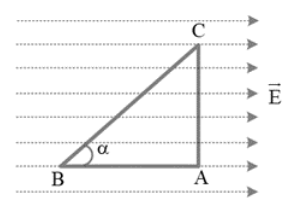
\includegraphics{../figs/VN11-2021-PH-TP006-3}
		\end{center}
	}
	
	\loigiai{
		Cường độ điện trường:
		$$U_\text{BC} = E \cdot \text{BC} \cdot \cos \alpha \Rightarrow E = \SI{8000}{V/m}.$$
		
		Hiệu điện thế $U_\text{AC}$:
		$$U_\text{AC} = E \cdot \text{AC} \cdot \cos 90^\circ = 0.$$
		
		Hiệu điện thế $U_\text{BA}$:
		$$U_\text{BA} = U_\text{BC} + U_\text{CA} = \SI{400}{V}.$$
	}
	
\end{enumerate}
\stopcontents[mychapters]
\setcounter{mychapter}{5}
\mychapter{Tụ điện}
\startcontents[mychapters]
\printcontents[mychapters]{}{0}{\setcounter{tocdepth}{1}}
\whiteBGstarBegin
\setcounter{section}{0}
\section{Trắc nghiệm}
\begin{enumerate}[label=\bfseries Câu \arabic*:]
	
	
	\item \mkstar{1}
	
	\cauhoi
	{Chọn câu \textbf{sai}.
		\begin{mcq}
			\item Khi nối hai bản tụ vào hai cực của một nguồn điện không đổi thì cả hai bản tụ đều mất điện tích.
			\item Nếu tụ điện đã được tích điện thì điện tích trên hai bản tụ luôn trái dấu và bằng nhau về độ lớn.
			\item Hai bản tụ phải được cách điện với nhau.
			\item Các bản tụ điện phẳng phải là những tấm vật dẫn phẳng đặt song song và cách điện với nhau.
		\end{mcq}
		
	}
	\loigiai
	{	\textbf{Đáp án: A.}
		
		Khi nối hai bản tụ vào hai cực của một nguồn điện không đổi thì hai bản tụ được tích điện, điện tích trên hai bản tụ luôn trái dấu và bằng nhau về độ lớn.
	}
	\item \mkstar{1}
	
	\cauhoi
	{Quy đổi $\SI{1}{nF}$ bằng
		\begin{mcq}(4)
			\item $\SI{e-9}{F}$.
			\item $\SI{e-12}{F}$.
			\item $\SI{e-6}{F}$.
			\item $\SI{e-3}{F}$.
		\end{mcq}
		
	}
	\loigiai
	{	\textbf{Đáp án: A.}
		
		Quy đổi $\SI{1}{nF} = \SI{e-9}{F}$.
	}
	\item \mkstar{2}
	
	\cauhoi
	{Sau khi ngắt tụ điện phẳng ra khỏi nguồn điện, ta tịnh tiến hai bản để khoảng cách giữa chúng tăng lên 2 lần. Điện tích của tụ sẽ
		\begin{mcq}(4)
			\item không đổi.
			\item giảm 2 lần.
			\item tăng 2 lần.
			\item tăng 4 lần.
		\end{mcq}
		
	}
	\loigiai
	{	\textbf{Đáp án: A.}
		
	}
	\item \mkstar{2}
	
	\cauhoi
	{Trên vỏ của một tụ điện có ghi $\SI{20}{\micro F}\ -\ \SI{200}{V}$. Nối hai bản tụ điện với một hiệu điện thế $\SI{120}{V}$. Điện tích của tụ điện là
		\begin{mcq}(4)
			\item $\SI{12e-4}{C}$.
			\item $\SI{24e-4}{C}$.
			\item $\SI{2e-3}{C}$.
			\item $\SI{4e-3}{C}$.
		\end{mcq}
		
	}
	\loigiai
	{	\textbf{Đáp án: B.}
		
		Áp dụng công thức:
		$$Q=CU=\SI{24e-4}{C}.$$
	}
	\item \mkstar{2}
	
	\cauhoi
	{Ghép như thế nào ba tụ $C_1=\SI{1}{mF}$, $C_2=\SI{2}{mF}$, $C_3=\SI{6}{mF}$ để tạo thành bộ tụ có điện dung là $\SI{9}{mF}$?
		\begin{mcq}
			\item Ghép nối tiếp ba tụ.
			\item Ghép ($C_1$ song song $C_3$) nối tiếp $C_2$.
			\item Ghép ($C_2$ song song $C_3$) nối tiếp $C_1$.
			\item Ghép song song ba tụ.
		\end{mcq}
		
	}
	\loigiai
	{	\textbf{Đáp án: D.}
		
		Ghép song song ba tụ thì tạo thành bộ tụ có điện dung là $C=C_1+C_2+C_3$.
	}
	\item \mkstar{2}
	
	\cauhoi
	{Hai tụ điện chứa cùng một lượng điện tích thì
		\begin{mcq}
			\item chúng có cùng điện dung.
			\item chúng có cùng hiệu điện thế.
			\item tụ điện có điện dung lớn hơn thì có hiệu điện thế lớn hơn.
			\item tụ điện có điện dung nhỏ hơn thì có hiệu điện thế lớn hơn.
		\end{mcq}
		
	}
	\loigiai
	{	\textbf{Đáp án: D.}
		
		Dựa vào công thức $Q=CU$, với hai tụ điện chứa cùng một lượng điện tích thì tụ điện có điện dung nhỏ hơn thì có hiệu điện thế lớn hơn.
	}
	\item \mkstar{2}
	
	\cauhoi
	{Một tụ điện có điện dung $\SI{2}{\micro F}$. Khi đặt một hiệu điện thế 4 V vào hai bản của tụ điện thì điện tích của tụ điện là
		\begin{mcq}(4)
			\item $\SI{2e-6}{C}$.
			\item $\SI{8e-6}{C}$.
			\item $\SI{8e-6}{\micro C}$.
			\item $\SI{4e-6}{C}$.
		\end{mcq}
		
	}
	\loigiai
	{	\textbf{Đáp án: B.}
		
		Áp dụng công thức:
		$$Q=CU = \SI{8e-6}{C}.$$
	}
	\item \mkstar{2}
	
	\cauhoi
	{Hai tụ điện có điện dung $C_1=2C_2$ mắc nối tiếp vào nguồn điện có hiệu điện thế $U$ thì mối quan hệ giữa $U_1$ và $U_2$ giữa hai tụ là
		\begin{mcq}(4)
			\item $U_1=2U_2$.
			\item $U_2=2U_1$.
			\item $U_2=3U_1$.
			\item $U_1=3U_2$.
		\end{mcq}
		
	}
	\loigiai
	{	\textbf{Đáp án: B.}
		
		Với đoạn mạch mắc nối tiếp thì $Q_1=Q_2$.
		
		Vì $C_1 = 2C_2$, áp dụng công thức $Q=CU$ thì được $U_2 = 2U_1$.
	}
	\item \mkstar{2}
	
	\cauhoi
	{Trường hợp nào say đây là một điều kiện cần để cho ta một tụ điện?
		\begin{mcq}
			\item Hai tấm gỗ khô đặt cách nhau một khoảng trong không khí.
			\item Hai tấm nhôm đặt cách nhau một khoảng trong nước nguyên chất.
			\item Hai tấm kẽm ngâm trong dung dịch axit.
			\item Hai tấm nhựa phủ ngoài một lá nhôm.
		\end{mcq}
		
	}
	\loigiai
	{	\textbf{Đáp án: B.}
	
	}
	\item \mkstar{2}
	
	\cauhoi
	{Giữa hai bản tụ phẳng cách nhau 1 cm có hiệu điện thế 10 V. Điện trường đều trong tụ có cường độ là
		\begin{mcq}(4)
			\item 100 V/m.
			\item 1 kV/m.
			\item 10 V/m.
			\item $\SI{0.01}{V/m}$.
		\end{mcq}
		
	}
	\loigiai
	{	\textbf{Đáp án: B.}
		
		Áp dụng công thức:
		$$E=\dfrac{U}{d} = \SI{1}{kV/m}.$$
	}
	\item \mkstar{2}
	
	\cauhoi
	{Nếu đặt vào hai đầu tụ điện một hiệu điện thế 4 V thì tích được cho tụ một điện lượng $\SI{2}{\micro C}$. Nếu đặt vào hai đầu tụ một hiệu điện thế 10 V thì tích được cho tụ một điện lượng là
		\begin{mcq}(4)
			\item $\SI{50}{\micro C}$.
			\item $\SI{1}{\micro C}$.
			\item $\SI{5}{\micro C}$.
			\item $\SI{0.8}{\micro C}$.
		\end{mcq}
		
	}
	\loigiai
	{	\textbf{Đáp án: C.}
		
		Lập tỉ lệ:
		$$\dfrac{Q_1}{Q_2} = \dfrac{U_1}{U_2} \Rightarrow Q_2 = \SI{5}{\micro C}.$$
	}
	\item \mkstar{2}
	
	\cauhoi
	{Bốn tụ điện có điện dung giống nhau ($C$) được ghép nối tiếp với nhau thành một bộ tụ. Điện dung của bộ tụ điện đó là
		\begin{mcq}(4)
			\item $C_\text{b} = 4C$.
			\item $C_\text{b} = \dfrac{C}{4}$.
			\item $C_\text{b} = 2C$.
			\item $C_\text{b} = \dfrac{C}{2}$.
		\end{mcq}
		
	}
	\loigiai
	{	\textbf{Đáp án: B.}
		
		Điện dung của bộ tụ gồm 4 tụ điện mắc nối tiếp: $C_\text{b} = \dfrac{C}{4}$.
	}
	\item \mkstar{2}
	
	\cauhoi
	{Bốn tụ điện có điện dung giống nhau ($C$) được ghép song song với nhau thành một bộ tụ. Điện dung của bộ tụ điện đó là
		\begin{mcq}(4)
			\item $C_\text{b} = 4C$.
			\item $C_\text{b} = \dfrac{C}{4}$.
			\item $C_\text{b} = 2C$.
			\item $C_\text{b} = \dfrac{C}{2}$.
		\end{mcq}
		
	}
	\loigiai
	{	\textbf{Đáp án: A.}
		
		Điện dung của bộ tụ gồm 4 tụ điện mắc song song: $C_\text{b} = 4C$.
	}
	\item \mkstar{2}
	
	\cauhoi
	{Một tụ điện phẳng, giữ nguyên diện tích $S$ của bản, tăng khoảng cách giữa hai bản lên 2 lần thì điện dung của tụ điện
		\begin{mcq}(4)
			\item không đổi.
			\item tăng 2 lần.
			\item giảm 2 lần.
			\item tăng 4 lần.
		\end{mcq}
		
	}
	\loigiai
	{	\textbf{Đáp án: C.}
		
		Dựa vào công thức $C=\dfrac{\varepsilon S}{4\pi kd}$, nếu giữ nguyên diện tích mà tăng khoảng cách $d$ lên 2 lần thì $C$ giảm 2 lần.
	}
	\item \mkstar{2}
	
	\cauhoi
	{Một tụ điện phẳng có hai bản dạng hình tròn, bán kính 2 cm đặt trong không khí cách nhau 2 mm. Điện dung của tụ điện đó là
		\begin{mcq}(4)
			\item $\SI{0.87}{pF}$.
			\item $\SI{5.6}{pF}$.
			\item $\SI{1.2}{pF}$.
			\item $\SI{1.8}{pF}$.
		\end{mcq}
		
	}
	\loigiai
	{	\textbf{Đáp án: B.}
		
		Diện tích của một bản tụ:
		$$S=\pi R^2 = \SI{1.2566e-3}{m^2}.$$
		
		Điện dung của tụ điện:
		$$C=\dfrac{\varepsilon S}{4\pi kd} \approx \SI{5.6}{pF}.$$
	}
	\item \mkstar{3}
	
	\cauhoi
	{Một bộ tụ gồm ba tụ giống nhau ghép song song và nối vào một nguồn điện không đổi có hiệu điện thế 20 V. Điện dung của bộ tụ bằng $\SI{1.5}{\micro F}$. Điện tích trên mỗi bản tụ có độ lớn là
		\begin{mcq}(4)
			\item $\SI{e-5}{C}$.
			\item $\SI{9e-5}{C}$.
			\item $\SI{3e-5}{C}$.
			\item $\SI{0.5e-7}{C}$.
		\end{mcq}
		
	}
	\loigiai
	{	\textbf{Đáp án: A.}
		
		Do ba tụ giống nhau ghép song song nên
		$$Q=Q_1+Q_2+Q_3=3Q_1=CU=\SI{3e-5}{C}.$$
		
		Vậy điện tích của mỗi bản tụ là
		$$Q_1=Q_2=Q_3=\dfrac{Q}{3} = \SI{e-5}{C}.$$
	}
	\item \mkstar{3}
	
	\cauhoi
	{Một tụ điện có điện dung $\SI{0.2}{\micro F}$ được nạp điện đến hiệu điện thế $\SI{100}{V}$. Điện tích và năng lượng của tụ điện là
		\begin{mcq}(2)
			\item $q=\SI{2e-5}{C}$, $W=\SI{e-3}{J}$.
			\item $q=\SI{2e5}{C}$, $W=\SI{e3}{J}$.
			\item $q=\SI{2e-5}{C}$, $W=\SI{2e-4}{J}$.
			\item $q=\SI{2e6}{C}$, $W=\SI{2e4}{J}$.
		\end{mcq}
		
	}
	\loigiai
	{	\textbf{Đáp án: A.}
		
		Điện tích:
		$$Q=CU = \SI{2e-5}{C}.$$
		
		Năng lượng:
		$$W=\dfrac{Q^2}{2C} = \SI{e-3}{J}.$$
	}
	\item \mkstar{3}
	
	\cauhoi
	{Một tụ điện có điện dung 24 nF được tích điện ở hiệu điện thế 450 V thì có bao nhiêu electron di chuyển đến bản tích điện âm của tụ?
		\begin{mcq}(4)
			\item $\SI{6.75e12}{}$.
			\item $\SI{13.3e12}{}$.
			\item $\SI{6.75e13}{}$.
			\item $\SI{13.3e13}{}$.
		\end{mcq}
		
	}
	\loigiai
	{	\textbf{Đáp án: C.}
		
		Điện tích của tụ nạp được:
		$$Q=CU = \SI{1.08e-5}{C}.$$
		
		Số electron di chuyển đến bản tụ:
		$$n=\dfrac{Q}{e} = \SI{6.75e13}{}.$$
	}
	\item \mkstar{3}
	
	\cauhoi
	{Hai tụ điện có điện dung $C_1=\SI{0.4}{\micro F}$, $C_2=\SI{0.6}{\micro F}$ ghép song song với nhau. Mắc bộ tụ điện đó vào nguồn điện có hiệu điện thế $U < \SI{60}{V}$ thì một trong hai tụ điện đó tích điện $\SI{3e-5}{C}$. Hiệu điện thế của nguồn điện là
		\begin{mcq}(4)
			\item $\SI{75}{V}$.
			\item $\SI{50}{V}$.
			\item $\SI{7.5e-5}{V}$.
			\item $\SI{5e-4}{V}$.
		\end{mcq}
		
	}
	\loigiai
	{	\textbf{Đáp án: B.}
		
		Xét tụ điện $C_1$, nếu $Q_1=\SI{3e-5}{C}$ thì $U=\dfrac{Q_1}{C_1} = \SI{75}{V}$ (không thỏa mãn $U<\SI{60}{V}$);
		
		Xét tụ điện $C_2$, nếu $Q_2=\SI{3e-5}{}$ thì $U=\dfrac{Q_2}{C_2} = \SI{50}{V}$ (thỏa mãn $U< \SI{60}{V}$).
		
		Vậy $U=\SI{50}{V}$
	}
	\item \mkstar{4}
	
	\cauhoi
	{Một bộ tụ điện gồm 10 tụ điện giống nhau ($C=\SI{8}{\micro F}$) ghép nối tiếp với nhau. Bộ tụ điện được nối với hiệu điện thế không đổi $U=\SI{150}{V}$. Độ biến thiên năng lượng của bộ tụ điện khi có 1 tụ bị đánh thủng là
		\begin{mcq}(4)
			\item $\Delta W= \SI{9}{mJ}$.
			\item $\Delta W = \SI{10}{mJ}$.
			\item $\Delta W = \SI{19}{mJ}$.
			\item $\Delta W = \SI{1}{mJ}$.
		\end{mcq}
		
	}
	\loigiai
	{	\textbf{Đáp án: D.}
		
		Năng lượng của bộ 10 tụ điện:
		$$W_1=\dfrac{1}{2}C_1 U^2 = \dfrac{1}{2} \dfrac{C}{10} U^2 = \SI{9}{mJ}.$$
		
		Năng lượng của bộ 9 tụ điện (do 1 tụ bị đánh thủng):
		$$W_2=\dfrac{1}{2}C_2U^2 = \dfrac{1}{2}\dfrac{C}{9} U^2 = \SI{10}{mJ}.$$
		
		Độ biến thiên năng lượng:
		$$\Delta W = |W_1 - W_2| = \SI{1}{mJ}.$$
	}
\end{enumerate}

\whiteBGstarEnd

\loigiai
{
	\begin{center}
		\textbf{BẢNG ĐÁP ÁN}
	\end{center}
	\begin{center}
		\begin{tabular}{|m{2.8em}|m{2.8em}|m{2.8em}|m{2.8em}|m{2.8em}|m{2.8em}|m{2.8em}|m{2.8em}|m{2.8em}|m{2.8em}|}
			\hline
			1.A  & 2.A  & 3.A  & 4.B  & 5.A  & 6.D  & 7.B  & 8.B  & 9.B  & 10.B  \\
			\hline
			11.C  & 12.B  & 13.A  & 14.C  & 15.B  & 16.A  & 17.A  & 18.C  & 19.B  & 20.D  \\
			\hline
		\end{tabular}
	\end{center}
}
\section{Tự luận}
\begin{enumerate}[label=\bfseries Câu \arabic*:]
	\item \mkstar{1}
	
	\cauhoi{
		Tụ điện là gì? Nêu công dụng của tụ điện và cách tích điện cho tụ điện.
	}
	
	\loigiai{
		Tụ điện là một hệ gồm hai vật dẫn đặt gần nhau và ngăn cách với nhau bằng một lớp cách điện (điện môi).
		
		Tụ điện dùng để tích điện, nhiệm vụ phóng điện và tích điện trong các mạch điện xoay chiều.
		
		Để tích điện cho tụ, người ta nối hai bản tụ với hai cực của nguồn điện. Bản tích điện dương nếu nối với cực dương của nguồn, bản tích điện âm nếu nối với cực âm của nguồn.
	}
	
	\item \mkstar{2}
	
	\cauhoi{
		Một tụ điện phẳng không khí có điện dung 1000 pF và khoảng cách giữa hai bản 1 mm. Tích điện cho tụ điện dưới hiệu điện thế 60 V. Điện tích của tụ điện và cường độ điện trường trong tụ là bao nhiêu?
	}
	
	\loigiai{
		Điện tích trong tụ:
		$$Q=CU=\SI{6e-8}{C}.$$
		
		Cường độ điện trường trong tụ:
		$$E=\dfrac{U}{d} = \SI{6e4}{V/m}.$$
	}
	\item \mkstar{3}
	
	\cauhoi{
		Một giọt dầu hình cầu nằm lơ lửng trong điện trường của một tụ điện phẳng không khí. Đường kính của giọt dầu là $\SI{0.5}{mm}$. Khối lượng riêng của dầu là $\SI{800}{kg/m^3}$. Bỏ qua lực đẩy Acsimet. Khoảng cách giữa hai bản tụ điện là 1 cm. Hiệu điện thế giữa hai bản tụ điện là 200 V, bản phía trên là bản dương đặt nằm ngang. Lấy $g=\SI{10}{m/s^2}$. Tính điện tích của giọt dầu.
	}
	
	\loigiai{
		Giọt dầu nằm cân bằng nên lực điện trường cân bằng với trọng lực. Vì trọng lực hướng thẳng đứng từ trên xuống nên lực điện trường có phương thẳng đứng hướng từ dưới lên. Vậy hạt bụi mang điện tích âm để $\vec F$ cùng phương, ngược chiều với $\vec E$.
		
		Độ lớn:
		$$|q|E = mg \Rightarrow |q| \dfrac{U}{d} = mg \Rightarrow |q| = \dfrac{mgd}{U} = \dfrac{V Dgd}{U}= \dfrac{4\pi R^3}{3} \dfrac{Dgd}{U} = \SI{23.8e-12}{C}.$$
		
	}
	\item \mkstar{4}
	
	\cauhoi{
		\begin{minipage}[l]{11cm}
			Tích điện cho tụ điện $C_1$ điện dung $\SI{20}{\micro F}$, dưới hiệu điện thế 300 V. Sau đó nối tụ điện $C_1$ với tụ điện $C_2$ có điện dung $\SI{10}{\micro F}$ chưa tích điện. Sau khi nối, điện tích trên các bản tụ $C_1$, $C_2$ lần lượt là $Q_1$ và $Q_2$. Tính $Q_1$ và $Q_2$.
		\end{minipage}
		\begin{minipage}[r]{5cm}
			\begin{center}
			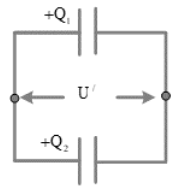
\includegraphics{../figs/VN11-2021-PH-TP007-1}
			\end{center}
		\end{minipage}
	}
	
	\loigiai{
	Điện tích được bảo toàn nên:	
		$$Q=Q' \Rightarrow (C_1 + C_2) U' = C_1 U \Rightarrow U' = \dfrac{U}{1+\dfrac{C_2}{C_1}} = \SI{200}{V}.$$
		
		Tìm được $Q_1=C_1U' = \SI{4e-3}{C}$; $Q_2=C_2U'=\SI{2e-3}{C}$.
	}
	\item \mkstar{4}
	
	\cauhoi{
		Một tụ điện phẳng có điện dung $C=\SI{4}{\micro F}$, khoảng cách giữa hai bản tụ là $d=\SI{4}{mm}$, được tích điện đến điện tích $Q=\SI{8e-4}{C}$, các bản tụ đặt song song theo phương thẳng đứng.
		\begin{enumerate}
			\item Tính hiệu điện thế giữa hai bản tụ;
			\item Một quả cầu kim loại có khối lượng $m=\SI{10}{g}$ tích điện $q=\SI{3}{\micro C}$ được treo bằng sợi dây nhẹ, không dãn, cách điện trong không gian giữa hai bản tụ. Xác định góc tạo bởi phương của dây treo và phương thẳng đứng khi quả cầu cân bằng. Lấy $g=\SI{10}{m/s^2}$.
		\end{enumerate}
	}
	
	\loigiai{
		\begin{enumerate}
			\item Tính hiệu điện thế giữa hai bản tụ;
			
			$$U=\dfrac{Q}{C} = \SI{200}{V}.$$
			
			\item Một quả cầu kim loại có khối lượng $m=\SI{10}{g}$ tích điện $q=\SI{3}{\micro C}$ được treo bằng sợi dây nhẹ, không dãn, cách điện trong không gian giữa hai bản tụ. Xác định góc tạo bởi phương của dây treo và phương thẳng đứng khi quả cầu cân bằng. Lấy $g=\SI{10}{m/s^2}$.
			
			Điều kiện cân bằng của quả cầu:
			$$\vec P + \vec F + \vec T = 0.$$
			
			Khi đó:
			$$\tan \alpha = \dfrac{F}{P} = \dfrac{|q|U}{mgd} \Rightarrow \alpha = 56^\circ .$$
		\end{enumerate}
		
	}
	
\end{enumerate}
\stopcontents[mychapters]
\chapter{Ôn tập: Chương I. Điện tích. Điện trường}
\whiteBGstarBegin
\setcounter{section}{0}
\section{Trắc nghiệm}
\begin{enumerate}[label=\bfseries Câu \arabic*:]
	
	
	\item \mkstar{1}
	
	\cauhoi
	{Chọn phát biểu đúng. Nhiễm điện do hưởng ứng xảy ra khi
		\begin{mcq}
			\item đưa một vật mang điện lại gần một vật dẫn điện đang trung hòa điện (đặt trên một giá cách điện).
			\item có electron dịch chuyển từ nguyên tử này sang nguyên tử khác, từ vật này sang vật khác.
			\item đưa một vật mang điện dương tiếp xúc với vật đang trung hòa điện.
			\item đưa một vật mang điện dương tiếp xúc với vật mang điện âm (đặt trên giá cách điện).
		\end{mcq}
		
	}
	\loigiai
	{	\textbf{Đáp án: A.}
		
		Nhiễm điện do hưởng ứng xảy ra khi đưa một vật mang điện lại gần vật dẫn điện đang trung hòa về điện.
	}
	\item \mkstar{1}
	
	\cauhoi
	{Chọn câu \textbf{sai}. Điện trường đều
		\begin{mcq}
			\item có cường độ như nhau tại mọi điểm.
			\item có đường sức là những đường song song cách đều nhau.
			\item xuất hiện giữa hai bản kim loại phẳng, song song và tích điện trái dấu.
			\item là điện trường tồn tại xung quanh điện tích điểm.
		\end{mcq}
		
	}
	\loigiai
	{	\textbf{Đáp án: D.}
		
		Điện trường đều là điện trường có cường độ như nhau tại mọi điểm, có đường sức là những đường thẳng song song cách đều nhau và xuất hiện giữa hai bản kim loại phẳng, song song và tích điện trái dấu.
	}
	\item \mkstar{1}
	
	\cauhoi
	{Phát biểu nào sau đây \textbf{không đúng}?
		\begin{mcq}
			\item Theo thuyết electron, một vật nhiễm điện dương là vật thiếu electron.
			\item Theo thuyết electron, một vật nhiễm điện âm là vật thừa electron.
			\item Theo thuyết electron, một vật nhiễm điện dương là vật đã nhận thêm các ion dương.
			\item Theo thuyết electron, một vật nhiễm điện âm là vật đã nhận thêm các electron.
		\end{mcq}
		
	}
	\loigiai
	{	\textbf{Đáp án: C.}
		
		Theo thuyết electron, một vật nhiễm điện dương là vật thiếu electron (mất electron), một vật nhiễm điện âm là vật thừa electron (nhận thêm electron).
	}
	\item \mkstar{1}
	
	\cauhoi
	{Trong các đại lượng vật lí sau, đại lượng nào là đại lượng vectơ?
		\begin{mcq}(2)
			\item Đường sức điện.
			\item Điện tích.
			\item Cường độ điện trường.
			\item Điện trường.
		\end{mcq}
		
	}
	\loigiai
	{	\textbf{Đáp án: C.}
		
		Cường độ điện trường là một đại lượng vectơ.
	}
	\item \mkstar{2}
	
	\cauhoi
	{Có hai điện tích điểm $q_1$ và $q_2$ đặt trong không khí, chúng hút nhau bằng một lực $F$. Khi đưa chúng vào trong dầu có hằng số điện môi $\varepsilon = 2$, vẫn giữ nguyên khoảng cách thì lực hút giữa chúng là
		\begin{mcq}(4)
			\item $F'=F$.
			\item $F'=2F$.
			\item $F'=F/2$.
			\item $F'=F/4$.
		\end{mcq}
		
	}
	\loigiai
	{	\textbf{Đáp án: C.}
		
		Lập tỉ lệ:
		$$\dfrac{F}{F'} = \dfrac{\varepsilon}{1} = 2 \Rightarrow F'=\dfrac{F}{2}.$$
	}
	\item \mkstar{2}
	
	\cauhoi
	{Khi một điện tích $q$ di chuyển trong một điện trường từ điểm A đến điểm B thì lực điện sinh công $\SI{4.5}{J}$. Nếu thế năng của $q$ tại A là $\SI{4.5}{J}$ thì thế năng tại B của nó là
		\begin{mcq}(4)
			\item $\SI{-4.5}{J}$.
			\item $\SI{-9}{J}$.
			\item $\SI{9}{J}$.
			\item $\SI{0}{J}$.
		\end{mcq}
		
	}
	\loigiai
	{	\textbf{Đáp án: D.}
		
	$$A_\text{AB} = W_\text A - W_\text B \Rightarrow W_\text B = \SI{0}{J}.$$
	}
	\item \mkstar{2}
	
	\cauhoi
	{Chọn câu đúng. Hai điện tích điểm đặt cách nhau một khoảng $r$. Dịch chuyển để khoảng cách giữa hai điện tích đó tăng lên 3 lần, nhưng vẫn giữ nguyên độ lớn điện tích của chúng. Khi đó lực tương tác giữa hai điện tích
		\begin{mcq}(2)
			\item tăng lên 3 lần.
			\item giảm đi 3 lần.
			\item tăng lên 9 lần.
			\item giảm đi 9 lần.
		\end{mcq}
		
	}
	\loigiai
	{	\textbf{Đáp án: D.}
		
		Lập tỉ số:
		$$\dfrac{F_1}{F_2} = \dfrac{3^2}{1} = 9 \Rightarrow F_2 = \dfrac{F_1}{9}.$$
	}
	\item \mkstar{2}
	
	\cauhoi
	{Chọn phát biểu đúng.
		\begin{mcq}
			\item Độ lớn của lực tương tác tĩnh điện giữa hai điện tích điểm tăng gấp 4 lần nếu khoảng cách giữa chúng tăng gấp đôi.
			\item Môi trường đặt hai điện tích điểm có hằng số điện môi càng lớn thì độ lớn của lực tương tác tĩnh điện giữa chúng càng lớn.
			\item Nếu độ lớn của một trong hai điện tích điểm tăng gấp đôi thì độ lớn lực tương tác tĩnh điện giữa chúng giảm đi một nửa.
			\item Độ lớn của lực tương tác tĩnh điện giữa hai điện tích điểm giảm đi 16 lần nếu khoảng cách giữa chúng tăng lên 4 lần.
		\end{mcq}
		
	}
	\loigiai
	{	\textbf{Đáp án: D.}
		
		Đáp án A sai vì lực tương tác tỉ lệ nghịch với khoảng cách $r$: $F$ tăng thì $r$ giảm;
		
		Đáp án B sai vì hằng số điện môi tỉ lệ nghịch với lực tương tác: $\varepsilon$ tăng thì $F$ giảm;
		
		Đáp án C sai vì lực tương tác tỉ lệ thuận với tích độ lớn của hai điện tích: độ lớn điện tích tăng thì $F$ tăng.
		.
	}
	\item \mkstar{2}
	
	\cauhoi
	{Một tụ điện có điện dung $\SI{5e-6}{F}$. Điện tích của tụ điện bằng $\SI{86}{\micro C}$. Hỏi hiệu điện thế trên hai bản tụ bằng bao nhiêu?
		\begin{mcq}(4)
			\item $U=\SI{27.2}{V}$.
			\item $U=\SI{37.2}{V}$.
			\item $U=\SI{47.2}{V}$.
			\item $U=\SI{17.2}{V}$.
		\end{mcq}
		
	}
	\loigiai
	{	\textbf{Đáp án: D.}
		
		Hiệu điện thế giữa hai bản tụ:
		$$U=\dfrac{Q}{C} = \SI{17.2}{V}.$$
	}
	\item \mkstar{2}
	
	\cauhoi
	{Có 4 vật A, B, C, D kích thước nhỏ, nhiễm điện. Biết rằng vật A hút vật B nhưng lại đẩy vật C. Vật C hút vật D. Khẳng định nào sau đây là \textbf{sai}?
		\begin{mcq}
			\item Điện tích của vật A và D cùng dấu.
			\item Điện tích của vật A và D trái dấu.
			\item Điện tích của vật B và D trái dấu.
			\item Điện tích của vật A và C cùng dấu.
		\end{mcq}
		
	}
	\loigiai
	{	\textbf{Đáp án: B.}
		
		Vật A hút vật B nên A trái dấu B;
		
		Vật A đẩy vật C nên A cùng dấu C;
		
		Vật C hút vật D nên C cùng dấu D.
		
		Suy ra A cùng dấu D, D khác dấu B.
	}
	\item \mkstar{2}
	
	\cauhoi
	{Tại một điểm có 2 cường độ điện trường thành phần vuông góc nhau và có độ lớn lần lượt là 3000 V/m và 4000 V/m. Độ lớn của cường độ điện trường tổng hợp là
		\begin{mcq}(4)
			\item 5000 V/m.
			\item 1000 V/m.
			\item 6000 V/m.
			\item 7000 V/m.
		\end{mcq}
		
	}
	\loigiai
	{	\textbf{Đáp án: A.}
		
		Với trường hợp hai vectơ cường độ điện trường thành phần vuông góc với nhau thì cường độ điện trường tổng hợp có độ lớn là
		$$E=\sqrt{E_1^2 + E_2^2} = \SI{5000}{V/m}.$$
	}
	\item \mkstar{3}
	
	\cauhoi
	{Một tụ điện không khí có điện dung 50 pF, khoảng cách giữa hai bản là 1 cm. Tính điện tích tối đa có thể tích cho tụ, biết rằng khi cường độ điện trường trong không khí lên đến $\SI{3e6}{V/m}$ thì không khí sẽ trở nên dẫn điện.
		\begin{mcq}(4)
			\item $\SI{15e4}{C}$.
			\item $\SI{15e-7}{C}$.
			\item $\SI{10e-7}{C}$.
			\item $\SI{3e-7}{C}$.
		\end{mcq}
		
	}
	\loigiai
	{	\textbf{Đáp án: B.}
		
		Điện tích tối đa trên một bản tụ là điện tích mà khi đó không khí vẫn còn là chất cách điện. Suy ra hiệu điện thế giữa hai bản tụ khi đó là
		$$U=Ed = \SI{3e4}{V}.$$
		
		Điện tích tối đa có thể tích cho tụ:
		$$Q=CU = \SI{15e-7}{C}.$$
	}
	\item \mkstar{3}
	
	\cauhoi
	{Cho hai điện tích $q_1=\SI{8e-8}{C}$, $q_2=\SI{2e-8}{C}$ lần lượt đặt tại hai điểm A và B cách nhau 10 cm trong chân không. Điểm M mà tại đó cường độ điện trường bằng 0 ở vị trí
		\begin{mcq}
			\item nằm trong khoảng AB, cách B là 10 cm.
			\item nằm trong khoảng AB, cách B là $\SI{3.3}{cm}$.
			\item nằm ngoài khoảng AB, cách A là 20 cm, cách B là 10 cm.
			\item nằm ngoài khoảng AB, cách A là 10 cm, cách B là 20 cm.
		\end{mcq}
		
	}
	\loigiai
	{	\textbf{Đáp án: B.}
		
		Để $\vec E = \vec E_\text{1M} + \vec E_\text{2M} = 0$ thì $\vec E_\text{1M} = -\vec E_\text{2M}$. Hệ quả: $\vec E_\text{1M}$ cùng phương, ngược chiều với $\vec E_\text{2M}$, còn về độ lớn thì $E_\text{1M} = E_\text{2M}$.
		
		Để $\vec E_\text{1M}$ cùng phương, ngược chiều với $\vec E_\text{2M}$ thì M phải nằm trong khoảng AB.
		
		Để $E_\text{1M} = E_\text{2M}$ thì $2\cdot \text{MB} = \text{AM}$. Suy ra $\text{MB} = \SI{3.3}{cm}$ và $\text{AM} = \SI{6.6}{cm}$.
		
		Vậy M nằm trong khoảng AB và cách B một khoảng $\SI{3.3}{cm}$.
	}
	\item \mkstar{3}
	
	\cauhoi
	{Trong không khí, người ta bố trí hai điện tích điểm có cùng độ lớn $\SI{1}{\micro C}$ nhưng trái dấu, cách nhau 2 m. Tại trung điểm của hai điện tích, cường độ điện trường là
		\begin{mcq}
			\item $\SI{18000}{V/m}$, hướng về điện tích dương.
			\item $\SI{18000}{V/m}$, hướng về điện tích âm.
			\item $\SI{0}{V/m}$.
			\item $\SI{18000}{V/m}$, hướng vuông góc với đoạn nối hai điện tích.
		\end{mcq}
		
	}
	\loigiai
	{	\textbf{Đáp án: B.}
		
		Biểu diễn vectơ cường độ điện trường thì thấy $\vec E = \vec E_1 + \vec E_2$ hướng về phía điện tích âm.
		\begin{center}
			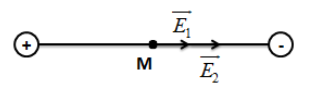
\includegraphics{../figs/VN11-2021-PH-TP011-1}
		\end{center}
	
	Độ lớn:
	$$E=E_1+E_2 = \SI{18000}{V/m}.$$
	}
	\item \mkstar{3}
	
	\cauhoi
	{Hai điện tích điểm $q_1=4q$ và $q_2=-q$ đặt tại hai điểm A, B cách nhau 9 cm trong chân không. Điểm M có cường độ điện trường bằng 0 cách B một khoảng
		\begin{mcq}(4)
			\item 27 cm.
			\item 9 cm.
			\item 18 cm.
			\item $\SI{4.5}{cm}$.
		\end{mcq}
		
	}
	\loigiai
	{	\textbf{Đáp án: B.}
		
	Do $q_1$ và $q_2$ trái dấu và $|q_1| > |q_2|$ nên vị trí cường độ điện trường tổng hợp bằng 0 nằm ngoài đoạn AB và ở phía B. Khi đó:
	$$E_1 = E_2 \Rightarrow k \dfrac{|4q|}{(r+9)^2} = k \dfrac{|-q|}{r^2} \Rightarrow r=\SI{9}{cm}.$$
	
	Điểm M có cường độ điẹn trường bằng 0 cách B một khoảng 9 cm.
	}
	\item \mkstar{3}
	
	\cauhoi
	{Một hạt bụi khối lượng $\SI{3.6e-15}{kg}$ nằm lơ lửng giữa hai tấm kim loại song song nằm ngang và nhiễm điện trái dấu. Điện tích của nó bằng $\SI{4.8e-18}{C}$. Tính độ lớn cường độ điện trường giữa hai tấm đó, lấy $g=\SI{10}{m/s^2}$.
		\begin{mcq}(4)
			\item $E=\SI{750}{V/m}$.
			\item $E=\SI{7500}{V/m}$.
			\item $E=\SI{75}{V/m}$.
			\item $E=\SI{1000}{V/m}$.
		\end{mcq}
		
	}
	\loigiai
	{	\textbf{Đáp án: B.}
		
		Để hạt bụi nằm cân bằng thì độ lớn lực điện $F$ bằng độ lớn trọng lực $P$:
		$$F=P \Rightarrow qE = mg \Rightarrow E = \dfrac{mg}{q} = \SI{7500}{V/m}.$$
	}
	\item \mkstar{3}
	
	\cauhoi
	{Một tụ điện phẳng được mắc vào hai cực của một nguồn điện có hiệu điện thế là $\SI{500}{V}$. Ngắt tụ điện ra khỏi nguồn rồi tăng khoảng cách giữa hai bản tụ lên 2 lần thì hiệu điện thế giữa hai bản của tụ điện đó
		\begin{mcq}(4)
			\item tăng 2 lần.
			\item tăng 4 lần.
			\item giảm 4 lần.
			\item giảm 2 lần.
		\end{mcq}
		
	}
	\loigiai
	{	\textbf{Đáp án: A.}
		
		Điện dung của tụ điện khi tăng khoagnr cách giữa hai bản lên 2 lần: $C'=\dfrac{C}{2}$.
		
		Mà $$Q=CU = C'U' \Rightarrow U'=\dfrac{C}{C'}U = 2U.$$
		
		Vậy $U$ tăng 2 lần.
	}
	\item \mkstar{3}
	
	\cauhoi
	{Đặt một điện tích thử $\SI{-1}{\micro C}$ tại một điểm thì nó chịu tác dụng của một lực điện $\SI{1}{mN}$ hướng từ trái qua phải. Cường độ điện trường tại vị trí đặt điện tích thử có độ lớn và chiều lần lượt là
		\begin{mcq}
			\item $\SI{1000}{V/m}$, hướng từ trái sang phải.
			\item $\SI{1}{V/m}$, hướng từ phải sang trái.
			\item $\SI{1}{V/m}$, hướng từ trái sang phải.
			\item $\SI{1000}{V/m}$, hướng từ phải sang trái.
		\end{mcq}
		
	}
	\loigiai
	{	\textbf{Đáp án: D.}
		
		Cường độ điện trường hướng từ phải sang trái (do $q<0$) và có độ lớn là
		$$E=\dfrac{F}{|q|} = \SI{1000}{V/m}.$$
	}
	\item \mkstar{3}
	
	\cauhoi
	{Ba điểm A, B, C tạo thành tam giác đều cạnh $a=\SI{100}{cm}$ nằm trong một điện trường đều $E=\SI{1000}{V/m}$, chiều từ B đến C. Hiệu điện thế $U_\text{CA}$ có giá trị bằng
		\begin{mcq}(4)
			\item $\SI{-500}{V}$.
			\item $\SI{-250}{V}$.
			\item $\SI{250}{V}$.
			\item $\SI{500}{V}$.
		\end{mcq}
		
	}
	\loigiai
	{	\textbf{Đáp án: A.}
		
		Hiệu điện thế $U_\text{CA}$:
		$$U_\text{CA} = Ea \cos 120^\circ = \SI{-500}{V}.$$
	}
	\item \mkstar{3}
	
	\cauhoi
	{Một electron bay từ điểm A đến điểm B trong điện trường, cho biết điện thế tại A là $V_\text{A} = \SI{150}{V}$, tại B là $V_\text{B} = \SI{50}{V}$. Độ biến thiên động năng của electron khi chuyển động từ A đến B là
		\begin{mcq}(4)
			\item $\SI{3.2e-17}{J}$.
			\item $\SI{-1.6e-17}{J}$.
			\item $\SI{1.6e-17}{J}$.
			\item $\SI{-3.2e-17}{J}$.
		\end{mcq}
		
	}
	\loigiai
	{	\textbf{Đáp án: B.}
		
		Độ biến thiên động năng bằng công của lực tĩnh điện:
		$$\Delta W_\text{đ} = A = qU_\text{AB} = q(V_\text{A} - V_\text{B}) = \SI{-1.6e-17}{J}.$$
	}
\end{enumerate}

\whiteBGstarEnd

\loigiai
{
	\begin{center}
		\textbf{BẢNG ĐÁP ÁN}
	\end{center}
	\begin{center}
		\begin{tabular}{|m{2.8em}|m{2.8em}|m{2.8em}|m{2.8em}|m{2.8em}|m{2.8em}|m{2.8em}|m{2.8em}|m{2.8em}|m{2.8em}|}
			\hline
			1.A  & 2.D  & 3.C  & 4.C  & 5.C  & 6.D  & 7.D  & 8.D  & 9.D  & 10.B  \\
			\hline
			11.A  & 12.B  & 13.B  & 14.B  & 15.B  & 16.B  & 17.A  & 18.D  & 19.A  & 20.B  \\
			\hline
		\end{tabular}
	\end{center}
}
\section{Tự luận}
\begin{enumerate}[label=\bfseries Câu \arabic*:]
	\item \mkstar{2}
	
	\cauhoi{
		Cho hai điện tích $q_1=\SI{2}{\micro C}$, $q_2=\SI{8}{\micro C}$ đặt tại hai điểm A và B trong chân không, với $\text{AB} = \SI{30}{cm}$. Xác định vị trí của điểm M để nếu đặt tại M một điện tích $q_0$ bất kì thì lực điện tổng hợp tác dụng lên $q_0$ bằng 0.
	}
	
	\loigiai{
		
		Vì $q_1$ và $q_2$ cùng dấu nên để lực điện tác dụng lên $q_0$ bằng 0 thì điểm đó phải nằm trên đoạn nối giữa $q_1$ và $q_2$. Khi đó:
		$$\vec F_{10} = - \vec F_{20}.$$
		
		Về độ lớn:
		$$F_{10} = F_{20} \Rightarrow k \dfrac{|q_1 q_0|}{r_1^2} = k \dfrac{|q_2 q_0|}{r_2^2}.$$
		
		Tìm được $r_1=\SI{10}{cm}$, $r_2=\SI{20}{cm}$.
	}
	
	\item \mkstar{2}
	
	\cauhoi{
		Tụ phẳng đặt trong không khí có điện dung $C=\SI{500}{pF}$, được tích điện đến hiệu điện thế $U=\SI{300}{V}$.
		\begin{enumerate}
			\item Tính điện tích $Q$ của tụ điện;
			\item Ngắt tụ điện ra khỏi nguồn. Nhúng tụ điện vào trong chất lỏng có $\varepsilon = 2$. Tính điện dung $C_1$, điện tích $Q_1$ và hiệu điện thế lúc đó;
			\item Vẫn nối tụ với nguồn. Nhúng tụ vào trong chất lỏng có $\varepsilon = 2$. Tính $C_2$, $Q_2$ và $U_2$ khi đó.
		\end{enumerate}
	}
	
	\loigiai{
		\begin{enumerate}
			\item Tính điện tích $Q$ của tụ điện;
			
			Điện tích của tụ:
			$$Q=CU = \SI{15e-8}{C}.$$
			
			\item Ngắt tụ điện ra khỏi nguồn. Nhúng tụ điện vào trong chất lỏng có $\varepsilon = 2$. Tính điện dung $C_1$, điện tích $Q_1$ và hiệu điện thế lúc đó;
			
			Khi ngắt tụ ra khỏi nguồn thì $Q$ không đổi nên điện tích của tụ lúc này là
			$$Q_1=Q=\SI{15e-8}{C}.$$
			
			Mà khi đó điện dung của tụ là
			$$C_1=2C = \SI{e-9}{F}.$$
			
			Vậy hiệu điện thế giữa hai bản tụ là
			$$U_1 = \dfrac{Q_1}{C_1} = \SI{150}{V}.$$
			
			\item Vẫn nối tụ với nguồn. Nhúng tụ vào trong chất lỏng có $\varepsilon = 2$. Tính $C_2$, $Q_2$ và $U_2$ khi đó.
			
			Khi vẫn nối tụ vào nguồn thì hiệu điện thế không đổi, khi đó hiệu điện thế giữa hai bản tụ là
			$$U_2 = U = \SI{300}{V}.$$
			
			Điện dung của tụ:
			$$C_2=2C = \SI{e-9}{F}.$$
			
			Điện tích của tụ:
			$$Q_2=C_2U_2 = \SI{3e-7}{C}.$$
		\end{enumerate}
		
	}
	\item \mkstar{2}
	
	\cauhoi{
		Đặt bốn điện tích âm có cùng độ lớn $q$ tại bốn đỉnh của một hình vuông ABCD cạnh $a$. Xác định cường độ điện trường tổng hợp tại giao điểm hai đường chéo của hình vuông.
	}
	
	\loigiai{
		Cường độ điện trường tại tâm O của hình vuông:
		$$\vec E_\text{O} = \vec E_\text{A} + \vec E_\text{B} + \vec E_\text{C} + \vec E_\text{D}.$$
		
		Độ lớn của các cường độ điện trường thành phần:
		$$E_\text{A} = E_\text{B} = E_\text{C} = E_\text{D} = k \dfrac{|q|}{\text{OA}^2}.$$
		
		Dễ thấy $\vec E_\text{AC} = \vec E_\text{A} + \vec E_\text{C} = 0$ và $\vec E_\text{BD} = \vec E_\text{B} + \vec E_\text{D} = 0$. Vậy cường độ điện trường tổng hợp tại O là
		$$\vec E_\text{O} = \vec E_\text{AC} + \vec E_\text{BD} = 0.$$
		
	}
	\item \mkstar{3}
	
	\cauhoi{
		Ba điểm A, B, C là ba đỉnh của một tam giác vuông tại A trong điện trường đều, cường độ $E=\SI{1000}{V/m}$. Đường sức điện trường song song với AC, chiều từ A đến C. Biết $\text{AC} = \SI{8}{cm}$, $\text{AB} = \SI{6}{cm}$.
		\begin{enumerate}
			\item Tính hiệu điện thế giữa các điểm A và B, A và C, B và C;
			\item Tính công của lực điện để dịch chuyển một electron từ điểm B đến điểm C;
			\item Một electron chuyển động không vận tốc đầu, xuất phát tại A, xác định vận tốc của electron đó khi nó di chuyển tới điểm C của tam giác đã cho.
		\end{enumerate}
	}
	
	\loigiai{
		\begin{enumerate}
			\item Tính hiệu điện thế giữa các điểm A và B, A và C, B và C;
			
			Vì điểm A và B nằm trên cùng một mặt đẳng thế nên $U_\text{AB} = 0$.
			
			Hiệu điện thế giữa A và C là
			$$U_\text{AC} = E \cdot \text{AC} = \SI{80}{V}.$$
			
			Hiệu điện thế giữa B và C là
			$$U_\text{BC} = E \cdot \text{BC} = \SI{100}{V}.$$
			\item Tính công của lực điện để dịch chuyển một electron từ điểm B đến điểm C;
			
			Công của lực điện:
			$$A=|e| \cdot U_\text{BC} = \SI{12.8e-8}{J}.$$
			
			\item Một electron chuyển động không vận tốc đầu, xuất phát tại A, xác định vận tốc của electron đó khi nó di chuyển tới điểm C của tam giác đã cho.
			
			Độ biến thiên động năng bằng công của lực điện:
			$$A_\text{AC} = W_\text{đ C} - W_\text{đ A} \Rightarrow v_\text{C} = \sqrt{\dfrac{2A_\text{AC}}{m}} = \SI{5.3e6}{m/s}.$$
		\end{enumerate}
		
	}
\end{enumerate}
\setcounter{mychapter}{6}
\mychapter{Dòng điện không đổi. Nguồn điện}
\startcontents[mychapters]
\printcontents[mychapters]{}{0}{\setcounter{tocdepth}{1}}
\whiteBGstarBegin
\setcounter{section}{0}
\section{Trắc nghiệm}
\begin{enumerate}[label=\bfseries Câu \arabic*:]
	
	
	\item \mkstar{1}
	
	\cauhoi
	{Phát biểu nào sau đây đúng?
		\begin{mcq}
			\item Nguồn điện là thiết bị tạo ra và duy trì hiệu điện thế nhằm duy trì dòng điện trong mạch. Trong nguồn điện dưới tác dụng của lực lạ, các điện tích dương di chuyển từ cực dương sang cực âm.
			\item Suất điện động của nguồn điện là đại lượng đặc trưng cho khả năng sinh công của nguồn điện và được đo bằng thương số giữa công của lực lạ thực hiện khi làm dịch chuyển một điện tích dương $q$ bên trong nguồn điện từ cực âm đến cực dương và độ lớn của điện tích $q$ đó.
			\item Suất điện động của nguồn điện là đại lượng đặc trưng cho khả năng sinh công của nguồn điện và được đo bằng thương số giữa công của lực lạ thực hiện khi làm dịch chuyển một điện tích âm $q$ bên trong nguồn điện từ cực âm đến cực dương và độ lớn của điện tích $q$ đó.
			\item Suất điện động của nguồn điện là đại lượng đặc trưng cho khả năng sinh công của nguồn điện và được đo bằng thương số giữa công của lực lạ thực hiện khi làm dịch chuyển một điện tích dương $q$ bên trong nguồn điện từ cực dương đến cực âm và độ lớn của điện tích $q$ đó.
		\end{mcq}
		
	}
	\loigiai
	{	\textbf{Đáp án: B.}
		
	}
	\item \mkstar{1}
	
	\cauhoi
	{Theo quy ước, chiều dòng điện là
		\begin{mcq}
			\item chiều dịch chuyển của các electron.
			\item chiều dịch chuyển của các điện tích dương.
			\item chiều dịch chuyển của các ion.
			\item chiều dịch chuyển của điện tích.
		\end{mcq}
		
	}
	\loigiai
	{	\textbf{Đáp án: B.}
		
	}
	\item \mkstar{2}
	
	\cauhoi
	{Suất điện động của một pin là $\SI{1.5}{V}$. Công của lực lạ khi dịch chuyển điện tích 2 C từ cực âm tới cực dương bên trong nguồn điện là
		\begin{mcq}(4)
			\item $\SI{3}{J}$.
			\item $\SI{4.5}{J}$.
			\item $\SI{4.3}{J}$.
			\item $\SI{0.75}{J}$.
		\end{mcq}
		
	}
	\loigiai
	{	\textbf{Đáp án: A.}
		
		Công của lực lạ:
		$$A=qU=\SI{3}{J}.$$
	}
	\item \mkstar{2}
	
	\cauhoi
	{Trên dây dẫn kim loại có một dòng điện không đổi chạy qua có cường độ $\SI{1.6}{mA}$. Trong 1 phút, số electron chuyển qua một tiết diện thẳng của dây là
		\begin{mcq}(4)
			\item $\SI{6e20}{}$.
			\item $\SI{6e19}{}$.
			\item $\SI{6e18}{}$.
			\item $\SI{6e17}{}$.
		\end{mcq}
		
	}
	\loigiai
	{	\textbf{Đáp án: D.}
		
		Áp dụng công thức:
		$$I=\dfrac{\Delta q}{\Delta t} = \dfrac{ne}{\Delta t} \Rightarrow n = \SI{6e17}{}.$$
	}
	\item \mkstar{2}
	
	\cauhoi
	{Lực lạ thực hiện một công 840 mJ khi dịch chuyển một điện tích $\SI{7e-2}{C}$ giữa hai cực bên trong một nguồn điện. Suất điện động của nguồn điện này là
		\begin{mcq}(4)
			\item 9 V.
			\item 10 V.
			\item 12 V.
			\item 15 V.
		\end{mcq}
		
	}
	\loigiai
	{	\textbf{Đáp án: C.}
		
		Suất điện động của nguồn:
		$$\calE = \dfrac{A}{q} = \SI{12}{V}.$$
	}
	\item \mkstar{2}
	
	\cauhoi
	{Một dòng điện không đổi, sau 2 phút có điện lượng 24 C chuyển qua một tiết diện thẳng. Cường độ dòng điện đó là
		\begin{mcq}(4)
			\item 12 A.
			\item $\SI{0.083}{A}$.
			\item $\SI{0.2}{A}$.
			\item 48 A.
		\end{mcq}
		
	}
	\loigiai
	{	\textbf{Đáp án: C.}
		
		Cường độ dòng điện:
		$$I=\dfrac{\SI{24}{C}}{\SI{120}{s}} = \SI{0.2}{C/s} = \SI{0.2}{A}.$$
	}
	\item \mkstar{2}
	
	\cauhoi
	{Con số $\SI{1.5}{V}$ ghi trên viên pin cho ta biết
		\begin{mcq}(2)
			\item công suất tiêu thụ của viên pin.
			\item điện trở trong của viên pin.
			\item suất điện động của viên pin.
			\item dòng điện viên pin tạo ra.
		\end{mcq}
		
	}
	\loigiai
	{	\textbf{Đáp án: C.}
		
		Con số $\SI{1.5}{V}$ ghi trên viên pin cho ta biết suất điện động của viên pin.
	}
	\item \mkstar{2}
	
	\cauhoi
	{Dòng điện không đổi chạy qua tiết diện của dây dẫn có cường độ $\SI{1.5}{A}$. Trong khoảng thời gian 3 s, điện lượng chuyển qua tiết diện thẳng của dây là
		\begin{mcq}(4)
			\item $\SI{4.5}{C}$.
			\item $\SI{0.5}{C}$.
			\item 2 C.
			\item 4 C.
		\end{mcq}
		
	}
	\loigiai
	{	\textbf{Đáp án: A.}
		
		Điện lượng chuyển qua tiết diện thẳng của dây:
		$$I=\dfrac{\Delta q}{\Delta t} \Rightarrow \Delta q=\SI{4.5}{C}.$$
	}
	\item \mkstar{2}
	
	\cauhoi
	{Một bộ nguồn gồm hai nguồn điện ($\varepsilon_1 = \SI{5}{V}$, $r_1=\SI{3}{\Omega}$, $\varepsilon_2 = \SI{7}{V}$, $r_2=\SI{5}{\Omega}$) mắc nối tiếp. Suất điện động của bộ nguồn là
		\begin{mcq}(4)
			\item 6 V.
			\item 2 V.
			\item 12 V.
			\item 7 V.
		\end{mcq}
		
	}
	\loigiai
	{	\textbf{Đáp án: C.}
		
		Suất điện động của bộ nguồn mắc nối tiếp:
		$$\varepsilon = \varepsilon_1 + \varepsilon_2 = \SI{12}{V}.$$
	}
	\item \mkstar{2}
	
	\cauhoi
	{Dòng electron đập lên màn đèn hình có độ lớn bằng $\SI{200}{\micro A}$. Có bao nhiêu electron đập vào màn hình trong mỗi giây?
		\begin{mcq}(4)
			\item $\SI{8.5e14}{}$.
			\item $\SI{12.5e14}{}$.
			\item $\SI{1.25e14}{}$.
			\item $\SI{2.5e14}{}$.
		\end{mcq}
		
	}
	\loigiai
	{	\textbf{Đáp án: B.}
		
		Số electron đập vào màn hình trong mỗi giây:
		$$I=n|e| \Rightarrow n = \dfrac{I}{|e|} = \SI{12.5e14}{}.$$
	}
	\item \mkstar{2}
	
	\cauhoi
	{Công của lực lạ khi làm dịch chuyển điện lượng $q=\SI{1.5}{C}$ trong nguồn điện từ cực âm đến cực dương của nó là 18 J. Suất điện động của nguồn điện đó là
		\begin{mcq}(4)
			\item $\SI{1.2}{V}$.
			\item $\SI{12}{V}$.
			\item $\SI{2.7}{V}$.
			\item $\SI{27}{V}$.
		\end{mcq}
		
	}
	\loigiai
	{	\textbf{Đáp án: B.}
		
		Suất điện động của nguồn:
		$$\varepsilon = \dfrac{A}{q} = \SI{12}{V}.$$
	}
	\item \mkstar{2}
	
	\cauhoi
	{Một điện lượng bằng $\SI{0.5}{C}$ chạy trong một dây dẫn trong thời gian $\SI{0.5}{s}$. Cường độ dòng điện trong mạch bằng
		\begin{mcq}(4)
			\item $\SI{0.25}{A}$.
			\item $\SI{0.1}{A}$.
			\item 1 A.
			\item $\SI{0.02}{A}$.
		\end{mcq}
		
	}
	\loigiai
	{	\textbf{Đáp án: C.}
		
		Cường độ dòng điện trong mạch:
		$$I=\dfrac{\Delta q}{\Delta t} = \SI{1}{C/s} = \SI{1}{A}.$$
	}
	\item \mkstar{2}
	
	\cauhoi
	{Số electron dịch chuyển qua tiết diện thẳng của dây dẫn trong khoảng thời gian 2 s là $\SI{6.25e18}{}$ hạt. Cho $q_e=\SI{-1.6e-19}{C}$, dòng điện qua dây dẫn có cường độ là
		\begin{mcq}(4)
			\item 2 A.
			\item 1 A.
			\item $\SI{0.5}{A}$.
			\item $\SI{0.512}{A}$.
		\end{mcq}
		
	}
	\loigiai
	{	\textbf{Đáp án: C.}
		
		Cường độ dòng điện:
		$$I=\dfrac{\Delta q}{\Delta t} = \dfrac{n |q_e|}{\Delta t} = \SI{0.5}{A}.$$
	}
	\item \mkstar{2}
	
	\cauhoi
	{Đoạn mạch gồm điện trở $R_1=\SI{100}{\Omega}$ mắc song song với điện trở $R_2=\SI{300}{\Omega}$. Điện trở tương đương toàn mạch là
		\begin{mcq}(4)
			\item $R=\SI{75}{\Omega}$.
			\item $R=\SI{100}{\Omega}$.
			\item $R=\SI{150}{\Omega}$.
			\item $R=\SI{400}{\Omega}$.
		\end{mcq}
		
	}
	\loigiai
	{	\textbf{Đáp án: A.}
		
		Điện trở tương đương toàn mạch của đoạn mạch mắc song song:
		$$R=\dfrac{R_1 R_2}{R_1 + R_2} = \SI{75}{\Omega}.$$
	}
	\item \mkstar{2}
	
	\cauhoi
	{Xét một dòng điện không đổi có cường độ $I$ chạy qua một dây dẫn kim loại. Biết rằng điện lượng chuyển qua tiết diện thẳng của dây dẫn mỗi phút là 150 C. Cường độ dòng điện này là
		\begin{mcq}(4)
			\item $\SI{0.8}{A}$.
			\item $\SI{2.5}{A}$.
			\item $\SI{0.4}{A}$.
			\item $\SI{1.25}{A}$.
		\end{mcq}
		
	}
	\loigiai
	{	\textbf{Đáp án: B.}
		
		Cường độ dòng điện:
		$$I=\dfrac{\Delta q}{\Delta t} = \SI{2.5}{C/s} = \SI{2.5}{A}.$$
	}
	\item \mkstar{3}
	
	\cauhoi
	{Điện tích của electron là $\SI{-1.6e-19}{C}$, điện lượng chuyển qua tiết diện thẳng của dây dẫn trong 30 s là 15 C. Số electron chuyển qua tiết diện thẳng của dây dẫn trong 1 s là
		\begin{mcq}(4)
			\item $\SI{3.125e18}{}$.
			\item $\SI{9.375e19}{}$.
			\item $\SI{7.895e19}{}$.
			\item $\SI{2.632e18}{}$.
		\end{mcq}
		
	}
	\loigiai
	{	\textbf{Đáp án: A.}
		
		Cường độ dòng điện:
		$$I=\dfrac{\Delta q}{\Delta t} = \SI{0.5}{A}.$$
		
		Đây cũng là điện lượng chuyển qua tiết diện thẳng của dây dẫn trong $\SI{1}{s}$. Suy ra số electron là
		$$n=\dfrac{I}{e} = \SI{3.125e18}{}.$$
	}
	\item \mkstar{3}
	
	\cauhoi
	{Một dòng điện không đổi chạy qua dây tóc của một bóng đèn có cường độ $I=\SI{1.6}{mA}$. Tính điện lượng và số electron dịch chuyển qua tiết diện thẳng của dây tóc bóng đèn trong thời gian 5 phút.
		\begin{mcq}(2)
			\item $\SI{0.48}{C}$ và $\SI{3e17}{}$ electron.
			\item $\SI{0.48}{C}$ và $\SI{3e18}{}$ electron.
			\item $\SI{0.28}{C}$ và $\SI{4e17}{}$ electron.
			\item $\SI{0.28}{C}$ và $\SI{4e17}{}$ electron.
		\end{mcq}
		
	}
	\loigiai
	{	\textbf{Đáp án: B.}
		
		Điện lượng chuyển qua trong 5 phút:
		$$\Delta q = I \Delta t = \SI{0.48}{C}.$$
		
		Số electron chuyển qua trong 5 phút:
		$$n=\dfrac{\Delta q}{e} = \SI{3e18}{}.$$
	}
	\item \mkstar{3}
	
	\cauhoi
	{Một dòng điện không đổi có cường độ 3 A thì sau một khoảng thời gian, có điện lượng là 4 C chuyển qua một tiết diện thẳng. Nếu cũng trong khoảng thời gian đó, với dòng điện có cường độ $\SI{4.5}{A}$ thì có điện lượng chuyển qua tiết diện thẳng đó là
		\begin{mcq}(4)
			\item 4 C.
			\item 8 C.
			\item $\SI{4.5}{C}$.
			\item 6 C.
		\end{mcq}
		
	}
	\loigiai
	{	\textbf{Đáp án: D.}
		
		Lập tỉ số:
		$$\dfrac{I_2}{I_2} = \dfrac{q_1}{q_2} \Rightarrow q_2 = \SI{6}{C}.$$
	}
	\item \mkstar{3}
	
	\cauhoi
	{Qua một nguồn điện không đổi, để chuyển một điện lượng 10 C thì lực lạ phải sinh công 20 mJ. Để chuyển một điện lượng 15 C thì lực lạ phải sinh công là
		\begin{mcq}(4)
			\item 10 mJ.
			\item 15 mJ.
			\item 20 mJ.
			\item 30 mJ.
		\end{mcq}
		
	}
	\loigiai
	{	\textbf{Đáp án: D.}
		
		Lập tỉ số:
		$$\dfrac{A_1}{A_2}=\dfrac{q_1}{q_2} \Rightarrow A_2 = \SI{30}{mJ}.$$
	}
	\item \mkstar{4}
	
	\cauhoi
	{Một dòng điện không đổi có cường độ $I=\SI{4.8}{A}$ chạy qua một dây kim loại có tiết diện thẳng $S=\SI{1}{cm^2}$. Tính vận tốc trung bình trong chuyển động định hướng của electron, biết mật độ electron tự do là $n=\SI{3e28}{m^{-3}}$.
		\begin{mcq}(4)
			\item 10 mm/s.
			\item $\SI{0.01}{mm/s}$.
			\item $\SI{0.1}{mm/s}$.
			\item 1 mm/s.
		\end{mcq}
		
	}
	\loigiai
	{	\textbf{Đáp án: B.}
		
		Dựa vào đơn vị của các đại lượng, ta suy ra được công thức để tính vận tốc trung bình $v$:
		$$I=nvqS \Rightarrow v = \SI{0.01}{mm/s}.$$
	}
\end{enumerate}

\whiteBGstarEnd

\loigiai
{
	\begin{center}
		\textbf{BẢNG ĐÁP ÁN}
	\end{center}
	\begin{center}
		\begin{tabular}{|m{2.8em}|m{2.8em}|m{2.8em}|m{2.8em}|m{2.8em}|m{2.8em}|m{2.8em}|m{2.8em}|m{2.8em}|m{2.8em}|}
			\hline
			1.B  & 2.B  & 3.A  & 4.D  & 5.C  & 6.C  & 7.C  & 8.A  & 9.C  & 10.B  \\
			\hline
			11.B  & 12.C  & 13.C  & 14.A  & 15.B  & 16.A  & 17.B  & 18.D  & 19.D  & 20.B  \\
			\hline
		\end{tabular}
	\end{center}
}
\section{Tự luận}
\begin{enumerate}[label=\bfseries Câu \arabic*:]
	\item \mkstar{1}
	
	\cauhoi{
		Nêu định nghĩa của cường độ dòng điện. Ý nghĩa của đơn vị cường độ dòng điện (Ampe).
	}
	
	\loigiai{
		
		Cường độ dòng điện là đại lượng đặc trưng cho tác dụng mạnh, yếu của dòng điện. Nó được xác định bằng thương số của điện lượng $\Delta q$ dịch chuyển qua tiết diện thẳng của vật dẫn trong khoảng thời gian $\Delta t$ và khoảng thời gian $\Delta t$ đó.
		$$I=\dfrac{\Delta q}{\Delta t}.$$
		
		Đơn vị đo cường độ dòng điện là Ampe: 1 Ampe là cường độ dòng điện chạy trong dây dẫn khi có điện lượng là 1 Cu-lông chạy qua tiết diện dây trong 1 giây.
	}
	
	\item \mkstar{2}
	
	\cauhoi{
		Một ắcquy có suất điện động 24 V và điện trở trong $\SI{2}{\Omega}$ mắc vào mạch ngoài có điện trở $R=\SI{6}{\Omega}$. Tính hiệu điện thế mạch ngoài khi mạch hở.
	}
	
	\loigiai{
		
		Khi mạch hở thì hiệu điện thế mạch ngoài là suất điện động của nguồn:
		$$U=\calE = \SI{24}{V}.$$
	}
	\item \mkstar{3}
	
	\cauhoi{
		Một nguồn điện có suất điện động 8 V. Khi mắc nguồn điện này với một bóng đèn thành mạch kín thì nó cung cấp một dòng điện có cường độ $I$, biết công của nguồn điện trong thời gian 10 phút là 10 J. Tính cường độ dòng điện chạy trong mạch kín.
	}
	
	\loigiai{
		
		Công suất của nguồn:
		$$\calP = \dfrac{A}{t} = \dfrac{1}{60}\ \text{W}.$$
		
		Cường độ dòng điện:
		$$I=\dfrac{\calP}{\calE} \approx \SI{2.08}{mA}.$$
	}
	\item \mkstar{4}
	
	\cauhoi{
		Một dây dẫn hình trụ tiết diện ngang $S=\SI{10}{mm^2}$ có dòng điện $I=\SI{2}{A}$ chạy qua. Hạt mang điện trong dây dẫn là electron tự do có điện tích có độ lớn là $e=\SI{1.6e-19}{C}$. Biết vận tốc trung bình của electron trong chuyển động có hướng là $\SI{0.1}{mm/s}$. Tính mật độ hạt electron trong dây dẫn.
	}
	
	\loigiai{
		
		Áp dụng công thức:
		$$I=nvqS \Rightarrow n = \SI{1.25e28}{m^{-3}}.$$
	}
	\item \mkstar{4}
	
	\cauhoi{
		Người ta mắc hai cực của nguồn điện với một biến trở có thể thay đổi từ 0 đến vô cực. Khi giá trị của biến trở rất lớn thì hiệu điện thế giữa hai cực của nguồn điện là $\SI{4.5}{V}$. Giảm giá trị của biến trở đến khi cường độ dòng điện trong mạch là 2 A thì hiệu điện thế giữa hai cực của nguồn điện là 4 V. Tính suất điện động và điện trở trong của nguồn điện.
	}
	
	\loigiai{
		
		Khi giá trị của biến trở rất lớn thì hiệu điện thế giữa hai đầu mạch cũng là suất điện động của nguồn: $$\calE = \SI{4.5}{V}.$$
		
		Áp dụng công thức:
		$$\calE=I_r + U \Rightarrow r = \SI{0.25}{\Omega}.$$
	}
	
\end{enumerate}
\stopcontents[mychapters]
%\stopcontents[parts]
%\part[Dòng điện xoay chiều]{Đại cương về dòng điện xoay chiều}
%\startcontents[parts]
%\printcontents[parts]{}{0}{\setcounter{tocdepth}{0}}
\setcounter{mychapter}{7}
\mychapter{Điện năng. Công suất điện}
\startcontents[mychapters]
\printcontents[mychapters]{}{0}{\setcounter{tocdepth}{1}}
\whiteBGstarBegin
\setcounter{section}{0}
\section{Trắc nghiệm}
\begin{enumerate}[label=\bfseries Câu \arabic*:]
	
	
	\item \mkstar{1}
	
	\cauhoi
	{Chọn câu đúng. Điện năng tiêu thụ được đo bằng
		\begin{mcq}(2)
			\item Vôn kế.
			\item Công tơ điện.
			\item Ampe kế.
			\item Tĩnh điện kế.
		\end{mcq}
		
	}
	\loigiai
	{	\textbf{Đáp án: B.}
		
	}
	\item \mkstar{1}
	
	\cauhoi
	{Công suất điện được đo bằng đơn vị nào sau đây?
		\begin{mcq}(4)
			\item Jun (J).
			\item Oát (W).
			\item Niutơn (N).
			\item Culông (C).
		\end{mcq}
		
	}
	\loigiai
	{	\textbf{Đáp án: B.}
		
	}
	\item \mkstar{2}
	
	\cauhoi
	{Một bếp điện $\SI{115}{V}\ -\ \SI{1}{kW}$ bị cắm nhầm vào mạng điện 230 V được nối qua cầu chì chịu được dòng điện tối đa 15 A. Khi đó
		\begin{mcq}
			\item bếp điện sẽ có công suất tỏa nhiệt nhỏ hơn định mức.
			\item bếp điện sẽ có công suất tỏa nhiệt bằng định mức.
			\item bếp điện sẽ có công suất tỏa nhiệt lớn hơn định mức.
			\item dòng điện sẽ làm chảy cầu chì.
		\end{mcq}
		
	}
	\loigiai
	{	\textbf{Đáp án: D.}
		
		Dòng điện khi đó là
		$$I=\dfrac{U}{R} = \dfrac{U}{\dfrac{U_\text{đm}^2}{\calP}} \approx \SI{17.4}{A}.$$
		
		Vì giá trị trên vượt mức dòng điện tối đa, do đó sẽ làm chảy cầu chì.
	}
	\item \mkstar{2}
	
	\cauhoi
	{Hai bóng đèn Đ1 ($\SI{220}{V}\ -\ \SI{25}{W}$), Đ2 ($\SI{220}{V}\ -\ \SI{100}{W}$) khi sáng bình thường thì
		\begin{mcq}
			\item cường độ dòng điện qua Đ1 lớn gấp hai lần cường độ dòng điện qua Đ2.
			\item cường độ dòng điện qua Đ2 lớn gấp bốn lần cường độ dòng điện qua Đ1.
			\item cường độ dòng điện qua Đ1 bằng cường độ dòng điện qua Đ2.
			\item điện trở của Đ2 lớn gấp bốn lần điện trở của Đ1.
		\end{mcq}
		
	}
	\loigiai
	{	\textbf{Đáp án: B.}
		
		Khi sáng bình thường thì hiệu điện thế đặt vào hai đầu bóng đèn là $\SI{220}{V}$.
		
		Lập tỉ số:
		$$\dfrac{I_1}{I_2} = \dfrac{\calP_1}{\calP_2} = \dfrac{1}{4}.$$
		
		Vậy cường độ dòng điện qua Đ2 lớn gấp 4 lần cường độ dòng điện qua Đ1.
	}
	\item \mkstar{2}
	
	\cauhoi
	{Để đun sôi 2 lít nước bằng một ấm điện, người ta đã dùng hết $\SI{0.25}{}$ số điện. Điều này có nghĩa là
		\begin{mcq}(2)
			\item ta đã dùng $\SI{0.25}{kW/h}$ điện năng.
			\item ta đã dùng $\SI{0.25}{kWh}$ điện năng.
			\item ta đã dùng $\SI{0.25}{kW}$ điện năng.
			\item ta đã dùng $\SI{1.8e6}{J}$ điện năng.
		\end{mcq}
		
	}
	\loigiai
	{	\textbf{Đáp án: B.}
		
		$\SI{0.25}{}$ số điện ($\SI{0.25}{}$ kí điện) nghĩa là $\SI{0.25}{kWh}$ điện năng.
	}
	\item \mkstar{2}
	
	\cauhoi
	{Nếu đặt vào hai đầu điện trở $R$ một hiệu điện thế $U_1$ thì công suất của mạch là 10 W. Nếu đặt vào hai đầu điện trở $R$ một hiệu điện thế $U_2=2U_1$ thì công suất của mạch là
		\begin{mcq}(4)
			\item 5 W.
			\item 20 W.
			\item 40 W.
			\item 10 W.
		\end{mcq}
		
	}
	\loigiai
	{	\textbf{Đáp án: C.}
		
		Lập tỉ lệ:
		$$\dfrac{\calP_1}{\calP_2} = \dfrac{U_1^2}{U_2^2}=\dfrac{1}{4} \Rightarrow \calP_2 = 4\calP_1 = \SI{40}{W}.$$
	}
	\item \mkstar{2}
	
	\cauhoi
	{Trên một bóng đèn dây tóc có ghi $\SI{12}{V}\ -\ \SI{1.25}{A}$. Kết luận nào dưới đây là \textbf{sai}?
		\begin{mcq}
			\item Bóng đèn này luôn có công suất là 15 W khi hoạt động.
			\item Bóng đèn này chỉ có công suất là 15 W khi mắc vào hiệu điện thế 12 V.
			\item Bóng đèn này tiêu thụ điện năng 15 J trong 1 s khi hoạt động bình thường.
			\item Bóng đèn này có điện trở $\SI{9.6}{\Omega}$ khi hoạt động bình thường.
		\end{mcq}
		
	}
	\loigiai
	{	\textbf{Đáp án: A.}
		
		Khi bóng đèn hoạt động dưới hiệu điện thế $\SI{12}{V}$ thì tiêu thụ công suất định mức là
		$$\calP_\text{đm} = U_\text{đm} I_\text{đm} = \SI{15}{W}.$$
		
		Khi bóng đèn hoạt động dưới hiệu điện thế khác $\SI{12}{V}$ thì tiêu thụ công suất khác với công suất định mức.
		
		Vậy khi nói rằng "bóng đèn này luôn có công suất là $\SI{15}{W}$ khi hoạt động" là sai. 
	}
	\item \mkstar{2}
	
	\cauhoi
	{Trong đoạn mạch chỉ có điện trở thuần, với thời gian như nhau, nếu cường độ dòng điện giảm 2 lần thì nhiệt lượng tỏa ra trên mạch
		\begin{mcq}(2)
			\item tăng 2 lần.
			\item giảm 4 lần.
			\item tăng 4 lần.
			\item giảm còn $\dfrac{1}{2}$.
		\end{mcq}
		
	}
	\loigiai
	{	\textbf{Đáp án: B.}
		
		Nhiệt lượng tỏa ra:
		$$Q=I^2 Rt$$
		
		Khi $I$ giảm 2 lần thì $Q$ giảm 4 lần.
	}
	\item \mkstar{2}
	
	\cauhoi
	{Một bóng đèn loại 6 V - 6 W. Điện trở của bóng đèn này là
		\begin{mcq}(4)
			\item $\SI{1}{\Omega}$.
			\item $\SI{3}{\Omega}$.
			\item $\SI{4}{\Omega}$.
			\item $\SI{6}{\Omega}$.
		\end{mcq}
		
	}
	\loigiai
	{	\textbf{Đáp án: D.}
		
		Điện trở của bóng đèn:
		$$R=\dfrac{U_\text{đm}^2}{\calP_{\text{đm}}} = \SI{6}{\Omega}.$$
	}
	\item \mkstar{2}
	
	\cauhoi
	{Điện trở $R_1$ tiêu thụ một công suất $\calP$ khi được mắc vào hiệu điện thế $U$ không đổi. Nếu mắc nối tiếp $R_1$ với một điện trở $R_2$ rồi mắc vào hiệu điện thế $U$ nói trên thì công suất tiêu thụ trên $R_1$ so với lúc đầu sẽ
		\begin{mcq}(2)
			\item giảm.
			\item không đổi.
			\item tăng.
			\item có thể tăng hoặc giảm.
		\end{mcq}
		
	}
	\loigiai
	{	\textbf{Đáp án: A.}
		
		Khi mắc nối tiếp $R_1$ và $R_2$ thì điện trở tương đương của mạch tăng: $R=R_1 + R_2$.
		
		Khi đó cường độ dòng điện qua mạch giảm $\left(I=\dfrac{U}{R}\right)$, công suất tiêu thụ trên $R_1$ giảm $(\calP_1 = I^2 R_1)$.
	}
	\item \mkstar{2}
	
	\cauhoi
	{Dòng điện không đổi có cường độ 2 A chạy qua một điện trở $\SI{200}{\Omega}$. Nhiệt lượng tỏa ra trên điện trở đó trong 40 s là
		\begin{mcq}(4)
			\item 20 kJ.
			\item 30 kJ.
			\item 32 kJ.
			\item 16 kJ.
		\end{mcq}
		
	}
	\loigiai
	{	\textbf{Đáp án: C.}
		
		Nhiệt lượng tỏa ra trên điện trở:
		$$Q=I^2 R t = \SI{32000}{J} = \SI{32}{kJ}.$$
	}
	\item \mkstar{2}
	
	\cauhoi
	{Có hai điện trở gồm $R_1$ và $R_2$, với $R_1=2R_2$, mắc nối tiếp vào đoạn mạch có hiệu điện thế không đổi. Goi công suất tỏa nhiệt trên điện trở $R_1$ là $\calP_1$, công suất tỏa nhiệt trên điện trở $R_2$ là
		\begin{mcq}(4)
			\item $\calP_2 = 2 \calP_1$.
			\item $\calP_2 = \calP_1$.
			\item $\calP_2 = \dfrac{1}{2} \calP_1$.
			\item $\calP_2 = 4 \calP_1$.
		\end{mcq}
		
	}
	\loigiai
	{	\textbf{Đáp án: C.}
		
		Lập tỉ lệ:
		$$\dfrac{\calP_1}{\calP_2} = \dfrac{R_1}{R_2} = \dfrac{2}{1} \Rightarrow \calP_2 = \dfrac{1}{2} \calP_1.$$
	}
	\item \mkstar{2}
	
	\cauhoi
	{Một nguồn điện có suất điện động 3 V khi mắc với một bóng đèn tạo thành một mạch kín thì có dòng điện có cường độ là $\SI{0.2}{A}$. Khi đó, công suất của nguồn điện này là
		\begin{mcq}(4)
			\item 10 W.
			\item 30 W.
			\item $\SI{0.9}{W}$.
			\item $\SI{0.1}{W}$.
		\end{mcq}
		
	}
	\loigiai
	{	\textbf{Đáp án: C.}
		
		Công suất của nguồn điện:
		$$\calP = \calE I = \SI{0.9}{W}.$$
	}
	\item \mkstar{2}
	
	\cauhoi
	{Tính điện năng tiêu thụ khi dòng điện có cường độ 1 A chạy qua dây dẫn trong 1 giờ. Biết hiệu điện thế giữa hai đầu dây dẫn này là 6 V.
		\begin{mcq}(4)
			\item $\SI{21600}{J}$.
			\item $\SI{216000}{J}$.
			\item $\SI{2160}{J}$.
			\item $\SI{21600}{J}$.
		\end{mcq}
		
	}
	\loigiai
	{	\textbf{Đáp án: A.}
		
		Điện năng tiêu thụ:
		$$A=UI t = \SI{21600}{J}.$$
	}
	\item \mkstar{2}
	
	\cauhoi
	{Tính công suất tiêu thụ khi dòng điện có cường độ 1 A chạy qua dây dẫn trong 1 giờ. Biết hiệu điện thế giữa hai đầu dây dẫn này là 6 V.
		\begin{mcq}(4)
			\item $\SI{0.6}{W}$.
			\item $\SI{6}{W}$.
			\item $\SI{60}{W}$.
			\item $\SI{600}{W}$.
		\end{mcq}
		
	}
	\loigiai
	{	\textbf{Đáp án: B.}
		
		Công suất tiêu thụ:
		$$\calP = UI = \SI{6}{W}.$$
	}
	\item \mkstar{3}
	
	\cauhoi
	{Khi hai điện trở giống nhau mắc song song vào một hiệu điện thế $U$ không đổi thì công suất tiêu thụ của chúng là 20 W. Nếu mắc chúng nối tiếp nhau rồi mắc vào hiệu điện thế như trên thì công suất tiêu thụ lúc này là
		\begin{mcq}(4)
			\item 5 W.
			\item 10 W.
			\item 40 W.
			\item 80 W.
		\end{mcq}
		
	}
	\loigiai
	{	\textbf{Đáp án: A.}
		
		Do $U$ không đổi nên ta có tỉ số:
		$$\dfrac{\calP_1}{\calP_2} = \dfrac{R_2}{R_1} = \dfrac{2R}{R/2} = 4.$$
		
		Vậy $\calP_2 = \dfrac{\calP_1}{4} = \SI{5}{W}$.
	}
	\item \mkstar{3}
	
	\cauhoi
	{Hai bóng đèn có công suất định mức bằng nhau, hiệu điện thế định mức của chúng lần lượt là $U_1=\SI{110}{V}$ và $U_2=\SI{220}{V}$. Tỉ số điện trở của chúng là
		\begin{mcq}(4)
			\item $\dfrac{R_1}{R_2} = \dfrac{1}{2}$.
			\item $\dfrac{R_1}{R_2} = \dfrac{2}{1}$.
			\item $\dfrac{R_1}{R_2} = \dfrac{1}{4}$.
			\item $\dfrac{R_1}{R_2} = \dfrac{4}{1}$.
		\end{mcq}
		
	}
	\loigiai
	{	\textbf{Đáp án: C.}
		
		Do $\calP$ không đổi nên ta có tỉ số:
		$$\dfrac{R_1}{R_2} = \dfrac{U_1^2}{U_2^2} = \dfrac{1}{4}.$$
	}
	\item \mkstar{3}
	
	\cauhoi
	{Một chiếc pin điện thoại có ghi ($\SI{3.6}{V}\ -\ \SI{900}{mAh}$). Điện thoại sau khi sạc đầy, pin có thể dùng để nghe gọi liên tục trong $\SI{4.5}{h}$. Bỏ qua mọi hao phí, công suất điện tiêu thụ trung bình của điện thoại trong quá trình đó là
		\begin{mcq}(4)
			\item $\SI{3.6}{W}$.
			\item $\SI{0.36}{W}$.
			\item $\SI{0.72}{W}$.
			\item $\SI{7.2}{W}$.
		\end{mcq}
		
	}
	\loigiai
	{	\textbf{Đáp án: C.}
		
		Điện năng của pin có được khi đã sạc đầy là
		$$A = \SI{3.6}{V} \cdot \SI{900e-3}{A} \cdot \SI{3600}{s} = \SI{11664}{J}.$$
		
		Công suất tiêu thụ trung bình:
		$$\calP = \dfrac{A}{t} = \SI{0.72}{W}.$$
	}
	\item \mkstar{3}
	
	\cauhoi
	{Một ắcquy có suất điện động là 12 V, sinh ra một công 720 J khi dịch chuyển điện tích ở bên trong giữa hai cực của nó khi ắcquy này phát điện. Biết thời gian dịch chuyển điện lượng này là 5 phút. Cường độ dòng điện chạy qua ắcquy khi đó là
		\begin{mcq}(4)
			\item $\SI{0.2}{A}$.
			\item 2 A.
			\item $\SI{1.2}{A}$.
			\item 12 A.
		\end{mcq}
		
	}
	\loigiai
	{	\textbf{Đáp án: A.}
		
		Áp dụng công thức:
		$$A=\calE I t \Rightarrow I = \SI{0.2}{A}.$$
	}
	\item \mkstar{4}
	
	\cauhoi
	{Một quạt điện (loại đứng) sử dụng dòng điện với hiệu điện thế 220 V và dòng điện chạy qua quạt có cường độ $\SI{1.41}{A}$. Tính số tiền điện phải trả cho chiếc quạt này trong 30 ngày, mỗi ngày sử dụng 4 giờ. Cho biết đơn giá điện cho mỗi kWh điện là 1720 đồng và coi như quạt luôn hoạt động bình thường.
		\begin{mcq}(4)
			\item 62 000 đồng.
			\item 64 025 đồng.
			\item 32 000 đồng.
			\item 34 000 đồng.
		\end{mcq}
		
	}
	\loigiai
	{	\textbf{Đáp án: B.}
		
		Điện năng quạt sử dụng trong 1 giây:
		$$A=UI = \SI{310.2}{J}.$$
		
		Điện năng quạt sử dụng trong 4 giờ (mỗi ngày):
		$$A'=A \cdot \SI{14400}{s} = \SI{4466880}{J}.$$
		
		Điện năng quạt sử dụng trong 30 ngày:
		$$A'' = A' \cdot 30 = \SI{134e6}{J} = \SI{37.224}{kWh}.$$
		
		Số tiền điện phải trả là $\SI{64025}{}$ đồng.
	}
\end{enumerate}

\whiteBGstarEnd

\loigiai
{
	\begin{center}
		\textbf{BẢNG ĐÁP ÁN}
	\end{center}
	\begin{center}
		\begin{tabular}{|m{2.8em}|m{2.8em}|m{2.8em}|m{2.8em}|m{2.8em}|m{2.8em}|m{2.8em}|m{2.8em}|m{2.8em}|m{2.8em}|}
			\hline
			1.B  & 2.B  & 3.D  & 4.B  & 5.B  & 6.C  & 7.A  & 8.B  & 9.D  & 10.A  \\
			\hline
			11.C  & 12.C  & 13.C  & 14.A  & 15.B  & 16.A  & 17.C  & 18.C  & 19.A  & 20.B  \\
			\hline
		\end{tabular}
	\end{center}
}
\section{Tự luận}
\begin{enumerate}[label=\bfseries Câu \arabic*:]
	\item \mkstar{1}
	
	\cauhoi{
		Điện năng mà một mạch điện tiêu thụ được đo bằng công do lực nào thực hiện? Viết công thức tính điện năng tiêu thụ và công suất điện của một đoạn mạch khi có dòng điện chạy qua.
	}
	
	\loigiai{
		
		Điện năng mà một đoạn mạch tiêu thụ được đo bằng công của lực điện thực hiện.
		
		Công thức tính điện năng tiêu thụ: $A=qU = UI t$.
		
		Công thức tính công suất điện: $\calP = \dfrac{A}{t} = UI$.
	}
	
	\item \mkstar{2}
	
	\cauhoi{
		Tính điện năng tiêu thụ và công suất điện khi dòng điện có cường độ 1 A chạy qua dây dẫn trong 1 giờ, biết hiệu điện thế giữa hai đầu dây dẫn là 6 V.
	}
	
	\loigiai{
		
			Điện năng tiêu thụ của đoạn mạch:
		$$A=UI t = \SI{21600}{J}.$$
		
		Công suất điện:
		$$\calP = UI = \SI{6}{W}.$$
	}
	\item \mkstar{3}
	
	\cauhoi{
		Trên nhãn của một ấm điện có ghi 220 V - 1000 W.
		\begin{enumerate}
			\item Cho biết ý nghĩa của các chỉ số trên;
			\item Sử dụng ấm điện với hiệu điện thế 220 V để đun sôi 2 lít nước từ $\SI{25}{\celsius}$. Tính thời gian để đun sôi nước, biết hiệu suất của ấm là $90\%$ và nhiệt dung riêng của nước là $\SI{4190}{J/(kg K)}$.
		\end{enumerate}
	}
	
	\loigiai{
		
	\begin{enumerate}
		\item Cho biết ý nghĩa của các chỉ số trên;
		
		Số $\SI{220}{V}$ là điện áp định mức của ấm.
		
		Số $\SI{1000}{W}$ là công suất định mức của ấm khi hoạt động bình thường ở $\SI{220}{V}$.
		
		\item Sử dụng ấm điện với hiệu điện thế 220 V để đun sôi 2 lít nước từ $\SI{25}{\celsius}$. Tính thời gian để đun sôi nước, biết hiệu suất của ấm là $90\%$ và nhiệt dung riêng của nước là $\SI{4190}{J/(kg K)}$.
		
		Đổi $\SI{2}{l} \rightarrow \SI{2}{kg}$.
		
		Nhiệt lượng cần thiết để đun nước:
		$$Q_1 = mc\Delta t = \SI{628500}{J}.$$
		
		Năng lượng thực tế cần thiết để cung cấp cho ấm:
		$$Q_1 = \dfrac{Q_1}{H} = \SI{698333.3}{J}.$$
		
		Thời gian đun nước:
		$$\calP = \dfrac{Q_2}{t} \Rightarrow t = \SI{698.3}{s}.$$
	\end{enumerate}
	}
	\item \mkstar{4}
	
	\cauhoi{
		Hai bóng đèn có công suất định mức lần lượt là 25 W và 100 W đều làm việc bình thường ở hiệu điện thế 110 V. Khi mắc nối tiếp hai bóng đèn này vào mạng điện 220 V thì đèn nào sẽ dễ hỏng hơn?
	}
	
	\loigiai{
		
		Cường độ dòng điện định mức qua đèn 1:
		$$I_1 = \dfrac{\calP_1}{U_1} = \xsi{\dfrac{5}{2}}{A}.$$
		
		Cường độ dòng điện định mức qua đèn 2:
		$$I_2 = \dfrac{\calP_2}{U_2} = \xsi{\dfrac{20}{2}}{A}.$$
		
		Điện trở của đèn 1:
		$$R_1 = \dfrac{U_1^2}{\calP_1} = \SI{484}{\Omega}.$$
		
		Điện trở của đèn 2:
		$$R_2 = \dfrac{U_2^2}{\calP_2} = \SI{212}{\Omega}.$$
		
		Nếu mắc hai bóng đèn này vào mạng điện $\SI{220}{V}$ thì cường độ dòng điện qua mạch là
		$$I=\dfrac{U}{R_1 + R_2} = \xsi{\dfrac{8}{22}}{A}.$$
		
		Do $I_1 > I_2$ nên đèn 1 (đèn công suất $\SI{25}{W}$) sẽ dễ hỏng hơn.
	}
	\item \mkstar{4}
	
	\cauhoi{
		Giả sử hiệu điện thế đặt vào hai đầu bóng đèn 220 V - 100 W đột ngột tăng lên tới 240 V thì công suất điện của bóng đèn khi đó tăng hay giảm bao nhiêu phần trăm so với công suất định mức của nó? Cho rằng điện trở của bóng đèn luôn không đổi.
	}
	
	\loigiai{
		
		Điện trở của bóng đèn:
		$$R=\dfrac{U^2}{\calP} = \SI{484}{\Omega}.$$
		
		Khi hiệu điện thế tăng lên tới $\SI{240}{V}$ thì công suất của đèn khi đó là
		$$\calP' = \dfrac{U'^2}{R} = \SI{119}{W}.$$
		
		Phần trăm tăng lên của công suất:
		$$\Delta P = \dfrac{\calP' - \calP}{\calP} = \SI{19}{\percent}.$$
	}
	
\end{enumerate}
\stopcontents[mychapters]
\setcounter{mychapter}{8}
\mychapter{Định luật Ôm đối với toàn mạch}
\startcontents[mychapters]
\printcontents[mychapters]{}{0}{\setcounter{tocdepth}{1}}
\whiteBGstarBegin
\setcounter{section}{0}
\section{Trắc nghiệm}
\begin{enumerate}[label=\bfseries Câu \arabic*:]
	
	
	\item \mkstar{1}
	
	\cauhoi
	{Chọn câu đúng.
		\begin{mcq}
			\item Cường độ dòng điện trong mạch kín tỉ lệ nghịch với điện trở ngoài của nguồn.
			\item Cường độ dòng điện trong mạch kín tỉ lệ nghịch với suất điện động của nguồn.
			\item Cường độ dòng điện trong mạch kín tỉ lệ nghịch với điện trở trong của nguồn.
			\item Cường độ dòng điện trong mạch kín tỉ lệ nghịch với tổng điện trở toàn mạch.
		\end{mcq}
		
	}
	\loigiai
	{	\textbf{Đáp án: D.}
		
		Cường độ dòng điện trong mạch kín tỉ lệ nghịch với tổng điện trở toàn mạch:
		$$I=\dfrac{\calE}{R+r}.$$
	}
	\item \mkstar{1}
	
	\cauhoi
	{Công thức nào dưới đây là định luật Ôm toàn mạch?
		\begin{mcq}(2)
			\item $I=\dfrac{\calE}{R+r}$.
			\item $U_\text{AB} = \calE - Ir$.
			\item $U_\text{AB} = \calE + Ir$.
			\item $U_\text{AB} = I_\text{AB} (R+r) - \calE$.
		\end{mcq}
		
	}
	\loigiai
	{	\textbf{Đáp án: A.}
		
		Cường độ dòng điện trong mạch kín tỉ lệ nghịch với tổng điện trở toàn mạch:
		$$I=\dfrac{\calE}{R+r}.$$
	}
	\item \mkstar{2}
	
	\cauhoi
	{Một nguồn điện có suất điện động 10 V và điện trở trong $\SI{1}{\Omega}$. Mắc nguồn điện với điện trở ngoài $\SI{4}{\Omega}$. Cường độ dòng điện trong mạch có độ lớn bằng
		\begin{mcq}(4)
			\item 10 A.
			\item $\SI{2.5}{A}$.
			\item 2 A.
			\item 4 A.
		\end{mcq}
		
	}
	\loigiai
	{	\textbf{Đáp án: C.}
		
		Áp dụng công thức:
		$$I=\dfrac{\calE}{R+r} = \SI{2}{A}.$$
	}
	\item \mkstar{2}
	
	\cauhoi
	{Theo định luật Ôm toàn mạch, khi thay đổi điện trở ngoài $R$ thì đồ thị biểu diễn sự phụ thuộc của hiệu điện thế giữa hai cực của nguồn vào cường độ dòng điện trong mạch có dạng
		\begin{mcq}
			\item một đoạn thẳng đi qua gốc tọa độ.
			\item một phần của đường parabol.
			\item một phần của đường hyperbol.
			\item một đoạn thẳng không đi qua gốc tọa độ.
		\end{mcq}
		
	}
	\loigiai
	{	\textbf{Đáp án: D.}
		
	}
	\item \mkstar{2}
	
	\cauhoi
	{Một mạch điện gồm một nguồn điện là pin 9 V, điện trở trong $\SI{0.5}{\Omega}$ và mạch ngoài gồm hai điện trở $\SI{8}{\Omega}$ mắc song song. Cường độ dòng điện trong mạch kín là
		\begin{mcq}(4)
			\item 1 A.
			\item $\SI{0.5}{A}$.
			\item $\SI{4.5}{A}$.
			\item 2 A.
		\end{mcq}
		
	}
	\loigiai
	{	\textbf{Đáp án: D.}
		
		Điện trở mạch ngoài:
		$$R=\dfrac{R_0}{2} = \SI{4}{\Omega}.$$
		
		Áp dụng công thức:
		$$I=\dfrac{\calE}{R+r} = \SI{2}{A}.$$
	}
	\item \mkstar{2}
	
	\cauhoi
	{Một mạch điện gồm điện trở thuần $\SI{2}{\Omega}$ được mắc vào hiệu điện thế có giá trị $U=\SI{20}{V}$. Nhiệt lượng tỏa ra trên điện trở trong 10 s là
		\begin{mcq}(4)
			\item 20 J.
			\item 40 J.
			\item 2000 J.
			\item 400 J.
		\end{mcq}
		
	}
	\loigiai
	{	\textbf{Đáp án: D.}
		
		Nhiệt lượng tỏa ra trên điện trở:
		$$Q=I^2 Rt = \dfrac{U^2}{R}t = \SI{400}{J}.$$
	}
	\item \mkstar{2}
	
	\cauhoi
	{Một bóng đèn sợi đốt có ghi 220 V - 110 W. Cường độ dòng điện định mức qua bóng đèn là
		\begin{mcq}(4)
			\item 440 A.
			\item 2 A.
			\item $\SI{0.5}{A}$.
			\item $\SI{4.4}{A}$.
		\end{mcq}
		
	}
	\loigiai
	{	\textbf{Đáp án: C.}
		
		Cường độ dòng điện định mức qua bóng đèn:
		$$I_\text{đm} = \dfrac{\calP_\text{đm}}{U_\text{đm}} = \SI{0.5}{A}.$$
	}
	\item \mkstar{2}
	
	\cauhoi
	{Đối với mạch điện kín gồm nguồn điện có suất điện động $\calE$, điện trở trong không đáng kể. Mạch ngoài ra biến trở $R$. Khi tăng $R$ thì hiệu điện thế hai đầu $R$
		\begin{mcq}(2)
			\item luôn giảm.
			\item luôn tăng.
			\item không đổi.
			\item tăng rồi giảm.
		\end{mcq}
		
	}
	\loigiai
	{	\textbf{Đáp án: C.}
		
		Hiệu điện thế hai đầu điện trở $R$ là
		$$U=\calE - Ir.$$
		
		Vì $U$ không phụ thuộc $R$ nên khi $R$ tăng thì $U$ không đổi.
	}
	\item \mkstar{2}
	
	\cauhoi
	{Một bóng đèn có ghi 3 V - 3 W được mắc vào hai cực của một nguồn điện có điện trở trong $\SI{1}{\Omega}$ thì đèn sáng bình thường. Suất điện động của nguồn là
		\begin{mcq}(4)
			\item 6 V.
			\item 2 V.
			\item 4 V.
			\item 12 V.
		\end{mcq}
		
	}
	\loigiai
	{	\textbf{Đáp án: C.}
		
		Điện trở bóng đèn:
		$$R=\dfrac{U_\text{đm}^2}{\calP_\text{đm}} = \SI{3}{\Omega}.$$
		
		Cường độ dòng điện định mức qua đèn:
		$$I_\text{đm} = \dfrac{\calP_\text{đm}}{U_\text{đm}} = \SI{1}{A}.$$
		
		Suất điện động của nguồn điện:
		$$I_\text{đm} = \dfrac{\calE}{R+r} \Rightarrow \calE = \SI{4}{V}.$$
	}
	\item \mkstar{2}
	
	\cauhoi
	{Một acquy có suất điện động 12 V và điện trở trong $\SI{2}{\Omega}$ mắc với mạch ngoài gồm điện trở $R=\SI{6}{\Omega}$. Khi đoản mạch, cường độ dòng điện qua nguồn là
		\begin{mcq}(4)
			\item 6 A.
			\item $\SI{1.5}{A}$.
			\item 3 A.
			\item 2 A.
		\end{mcq}
		
	}
	\loigiai
	{	\textbf{Đáp án: A.}
		
		Khi đoản mạch thì điện trở mạch ngoài $R=0$, hiệu điện thế mạch ngoài $U=\calE$.
		
		Cường độ dòng điện khi đoản mạch:
		$$I=\dfrac{\calE}{r} = \SI{6}{A}.$$
	}
	\item \mkstar{2}
	
	\cauhoi
	{Hiệu điện thế giữa hai đầu đoạn mạch gồm $R_1=\SI{10}{\Omega}$ nối tiếp $R_2=\SI{30}{\Omega}$ là $U=\SI{20}{V}$. Cường độ dòng điện qua điện trở $R_1$ là
		\begin{mcq}(4)
			\item $\SI{0.5}{A}$.
			\item $\SI{0.67}{A}$.
			\item 1 A.
			\item 2 A.
		\end{mcq}
		
	}
	\loigiai
	{	\textbf{Đáp án: A.}
		
		Điện trở tương đương:
		$$R=R_1 + R_2 = \SI{40}{\Omega}.$$
		
		Cường độ dòng điện qua mạch:
		$$I= I_1 = I_2 = \dfrac{U}{R} = \SI{0.5}{A}.$$
	}
	\item \mkstar{2}
	
	\cauhoi
	{Hiệu điện thế giữa hai đầu đoạn mạch gồm $R_1=\SI{10}{\Omega}$ song song $R_2=\SI{30}{\Omega}$ là $U=\SI{20}{V}$. Cường độ dòng điện qua điện trở $R_1$ là
		\begin{mcq}(4)
			\item $\SI{0.5}{A}$.
			\item $\SI{0.67}{A}$.
			\item 1 A.
			\item 2 A.
		\end{mcq}
		
	}
	\loigiai
	{	\textbf{Đáp án: D.}
		
		Cường độ dòng điện qua điện trở $R_1$:
		$$I_1 = \dfrac{U}{R_1} = \SI{2}{A}.$$
	}
	\item \mkstar{2}
	
	\cauhoi
	{Hiệu điện thế giữa hai đầu đoạn mạch gồm $R_1=\SI{10}{\Omega}$ song song $R_2=\SI{30}{\Omega}$ là $U=\SI{20}{V}$. Cường độ dòng điện toàn mạch là
		\begin{mcq}(4)
			\item $\SI{1.5}{A}$.
			\item $\SI{2.67}{A}$.
			\item $\SI{0.5}{A}$.
			\item 2 A.
		\end{mcq}
		
	}
	\loigiai
	{	\textbf{Đáp án: B.}
		
		Điện trở tương đương:
		$$R=\dfrac{R_1 R_2}{R_1 + R_2} = \SI{7.5}{\Omega}.$$
		
		Cường độ dòng điện qua điện trở $R_1$:
		$$I=\dfrac{U}{R} = \SI{2.67}{A}.$$
	}
	\item \mkstar{2}
	
	\cauhoi
	{Hiệu điện thế giữa hai đầu đoạn mạch gồm bốn điện trở $\SI{6}{\Omega}$ mắc nối tiếp là $U=\SI{12}{V}$. Dòng điện chay qua mỗi điện trở bằng
		\begin{mcq}(4)
			\item $\SI{0.5}{A}$.
			\item 2 A.
			\item 8 A.
			\item 16 A.
		\end{mcq}
		
	}
	\loigiai
	{	\textbf{Đáp án: A.}
		
		Điện trở tương đương:
		$$R=4 \cdot \SI{6}{\Omega} = \SI{24}{\Omega}.$$
		
		Dòng điện qua mỗi điện trở:
		$$I=\dfrac{U}{R} = \SI{0.5}{A}.$$
	}
	\item \mkstar{2}
	
	\cauhoi
	{Gọi $\calE$ là suất điện động của nguồn, $\calE'$ là suất điện động của máy thu, $R$ là điện trở mạch ngoài, $r$ là điện trở trong của nguồn, $r'$ là điện trở trong của máy thu. Biểu thức định luật Ôm cho toàn mạch có chứa nguồn mà máy thu là
		\begin{mcq}(4)
			\item $I=\dfrac{\calE}{R}$.
			\item $I=\dfrac{\calE}{R+r+r'}$.
			\item $I=\dfrac{\calE + \calE'}{R+r+r'}$.
			\item $I=\dfrac{\calE - \calE'}{R+r+r'}$.
		\end{mcq}
		
	}
	\loigiai
	{	\textbf{Đáp án: D.}
		
		Biểu thức định luật Ôm cho toàn mạch có chứa nguồn và máy thu:
		$$I=\dfrac{\calE - \calE'}{R+r+r'}.$$
	}
	\item \mkstar{3}
	
	\cauhoi
	{Một nguồn điện có suất điện động 6 V, điện trở trong $\SI{2}{\Omega}$, mắc với mạch ngoài là một biến trở $R$ để tạo thành một mạch kín. Giá trị của $R$ để công suất tiêu thụ của mạch ngoài là 4 W là
		\begin{mcq}(4)
			\item $\SI{1}{\Omega}$.
			\item $\SI{2}{\Omega}$.
			\item $\SI{3}{\Omega}$.
			\item $\SI{4}{\Omega}$.
		\end{mcq}
		
	}
	\loigiai
	{	\textbf{Đáp án: A.}
		
		Áp dụng công thức:
		$$\calP = I^2 R = \left(\dfrac{\calE}{r+R}\right)^2 R \Rightarrow R = \SI{1}{\Omega}.$$
	}
	\item \mkstar{3}
	
	\cauhoi
	{Một mạch điện có điện trở ngoài bằng 5 lần điện trở trong. Khi xảy ra hiện tượng đoản mạch thì tỉ số giữa cường độ dòng điện đoản mạch và cường độ dòng điện không đoản mạch là
		\begin{mcq}(4)
			\item 4.
			\item 5.
			\item 6.
			\item vô cực.
		\end{mcq}
		
	}
	\loigiai
	{	\textbf{Đáp án: C.}
		
		Khi đoản mạch thì ta có:
		$$I_1 = \dfrac{\calE}{0+4}.$$
		
		Khi không đoản mạch thì ta có:
		$$I_2 = \dfrac{\calE}{5r + r} = \dfrac{\calE}{6r}.$$
		
		Vậy:
		$$\dfrac{I_1}{I_2} = 6.$$
	}
	\item \mkstar{3}
	
	\cauhoi
	{Biết rằng khi điện trở mạch ngoài của một mạch điện tăng từ $R_1=\SI{3}{\Omega}$ đến $R_2=\SI{10.5}{\Omega}$ thì hiệu điện thế giữa hai cực của nguồn tăng gấp hai lần. Điện trở trong của nguồn điện đó là
		\begin{mcq}(4)
			\item $\SI{7.5}{\Omega}$.
			\item $\SI{6.75}{\Omega}$.
			\item $\SI{10.5}{\Omega}$.
			\item $\SI{7}{\Omega}$.
		\end{mcq}
		
	}
	\loigiai
	{	\textbf{Đáp án: D.}
		
		Theo đề bài thì ta có:
		$$U_2 = 2U_1 \Rightarrow I_1 = \SI{1.75}{} I_2.$$
		
		Áp dụng định luật Ôm:
		$$\calE = I_1 (R_1 + r) = I_2 (R_2 +r).$$
		
		Giải hệ hai phương trình trên, tìm được $r=\SI{7}{\Omega}$.
	}
	\item \mkstar{3}
	
	\cauhoi
	{Cho mạch điện như hình vẽ.
		\begin{center}
			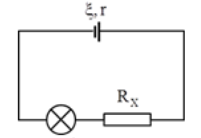
\includegraphics{../figs/VN11-2021-PH-TP014-1}
		\end{center}
	Biết $\calE = \SI{12}{V}$, $r=\SI{4}{\Omega}$, bóng đèn thuộc loại 6 V - 6 W. Để đèn sáng bình thường thì giá trị của $R_x$ là
		\begin{mcq}(4)
			\item $\SI{4}{\Omega}$.
			\item $\SI{2}{\Omega}$.
			\item $\SI{6}{\Omega}$.
			\item $\SI{12}{\Omega}$.
		\end{mcq}
		
	}
	\loigiai
	{	\textbf{Đáp án: B.}
		
		Điện trở của đèn:
		$$R_\text{đ} = \SI{6}{\Omega}.$$
		
		Cường độ dòng điện định mức của đèn:
		$$I_\text{đm} = \SI{1}{A}.$$
		
		Để đèn sáng bình thường thì
		$$I= I_\text{đm} \Rightarrow \dfrac{\calE}{R_x + R_\text{đ} + r} = 1 \Rightarrow R_x = \SI{2}{\Omega}.$$
	}
	\item \mkstar{4}
	
	\cauhoi
	{Cho mạch điện như hình vẽ.
		\begin{center}
			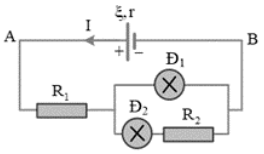
\includegraphics{../figs/VN11-2021-PH-TP014-1-2}
		\end{center}
	Cho biết $\calE = \SI{6.6}{V}$, điện trở trong $r=\SI{0.12}{\Omega}$, bóng đèn Đ1 loại 6 V - 3 W, bóng đèn Đ2 loại $\SI{2.5}{V}$ - $\SI{1.25}{W}$. Coi điện trở của bóng đèn không thay đổi. Các đèn sáng thế nào so với định mức?
		\begin{mcq}(2)
			\item Đ1 sáng yếu, Đ2 sáng mạnh.
			\item Đ1 sáng mạnh, Đ2 sáng yếu.
			\item Cả hai đèn đều sáng yếu.
			\item Cả hai đèn đều sáng mạnh.
		\end{mcq}
		
	}
	\loigiai
	{	\textbf{Đáp án: A.}
		
		Điện trở Đ1:
		$$R_\text{đ1} = \SI{12}{\Omega}.$$
		
		Điện trở Đ2:
		$$R_\text{đ2} = \SI{5}{\Omega}.$$
		
		Cường độ dòng điện định mức qua Đ1:
		$$I_\text{đ1} = \SI{0.5}{A}.$$
		
		Cường độ dòng điện định mức qua Đ2:
		$$I_\text{đ2} = \SI{0.5}{A}.$$
		
		Tính:
		$$R_\text{đ1-đ2-R2} = \SI{4}{\Omega} \Rightarrow R= R_1 + R_\text{đ1-đ2-R2} = \SI{4.48}{\Omega} \Rightarrow I = \dfrac{\calE}{R+r} = \xsi{\dfrac{33}{23}}{A}.$$
		
		Tính cường độ dòng điện qua mỗi đèn:
		$$I_1 = \dfrac{I \cdot R_\text{đ1-đ2-R2}}{R_\text{đ1}} = \xsi{\dfrac{11}{23}}{A}.$$
		
		$$I_2 = \dfrac{I \cdot R_\text{đ1-đ2-R2}}{R_\text{đ2}+R_2} = \xsi{\dfrac{22}{23}}{A}.$$
		
		Vậy đèn 1 sáng yếu hơn định mức và đèn 2 sáng mạnh hơn định mức.
	}
\end{enumerate}

\whiteBGstarEnd

\loigiai
{
	\begin{center}
		\textbf{BẢNG ĐÁP ÁN}
	\end{center}
	\begin{center}
		\begin{tabular}{|m{2.8em}|m{2.8em}|m{2.8em}|m{2.8em}|m{2.8em}|m{2.8em}|m{2.8em}|m{2.8em}|m{2.8em}|m{2.8em}|}
			\hline
			1.D  & 2.A  & 3.C  & 4.D  & 5.D  & 6.D  & 7.C  & 8.C  & 9.C  & 10.A  \\
			\hline
			11.A  & 12.D  & 13.B  & 14.A  & 15.D  & 16.A  & 17.C  & 18.D  & 19.B  & 20.A  \\
			\hline
		\end{tabular}
	\end{center}
}
\section{Tự luận}
\begin{enumerate}[label=\bfseries Câu \arabic*:]
	\item \mkstar{1}
	
	\cauhoi{
		Định luật Ôm đối với toàn mạch đề cập tới loại mạch điện kín nào? Phát biểu định luật và viết biểu thức của định luật.
	}
	
	\loigiai{
		
		Định luật Ôm đối với toàn mạch đề cập tới mạch điện gồm một nguồn điện $(\calE , r)$ mắc với các điện trở ngoài $R$.
		
		Phát biểu định luật: Cường độ dòng điện chạy trong mạch kín tỉ lệ thuận với suất điện động của nguồn điện và tỉ lệ nghịch với điện trở toàn phần của mạch đó.
		
		Biểu thức định luật: $$I=\dfrac{\calE}{R+r}.$$
	}
	
	\item \mkstar{2}
	
	\cauhoi{
		Điện trở trong của một ắcquy là $\SI{0.06}{\Omega}$ và trên vỏ của nó có ghi 12 V. Mắc vào hai cực của ắcquy này một bóng đèn có ghi 12 V - 5 W. Coi điện trở của bóng đèn không thay đổi. Hiệu suất của nguồn điện là bao nhiêu?
	}
	
	\loigiai{
		
		Điện trở trong của bóng đèn:
		$$R=\dfrac{U_\text{đm}^2}{\calP_\text{đm}}=\SI{28.8}{\Omega}.$$
		
		Hiệu suất của nguồn điện:
		$$H=\dfrac{I^2 R}{I^2 (R+r)} = \SI{99.8}{\percent}.$$
	}
	\item \mkstar{3}
	
	\cauhoi{
		Khi mắc điện trở $R_1=\SI{500}{\Omega}$ vào hai cực của một pin mặt trời thì hiệu điện thế mạch ngoài là $U_1=\SI{0.10}{V}$. Nếu thay điện trở $R_1$ bằng điện trở $R_2=\SI{1000}{\Omega}$ thì hiệu điện thế mạch ngoài bây giờ là $U_2=\SI{0.15}{V}$. Tính suất điện động và điện trở trong của pin.
	}
	
	\loigiai{
		
		Áp dụng định luật Ôm:
		$$U_R = IR = \dfrac{\calE}{1 + \dfrac{r}{R}}.$$
		
		Giải phương trình trên, tính được:
		$$\calE = \SI{0.3}{V};$$
		$$r=\SI{1000}{\Omega}.$$
	}
	\item \mkstar{4}
	
	\cauhoi{
		Mạch kín gồm nguồn điện $\calE = \SI{200}{V}$, $r=\SI{0.5}{\Omega}$ và hai điện trở $R_1=\SI{100}{\Omega}$, $R_2=\SI{500}{\Omega}$ mắc nối tiếp. Một Vôn kế không lí tưởng (có điện trở $R_V$) được mắc song song với $R_2$ thì số chỉ của nó là 160 V. Tìm số chỉ của Vôn kế nếu nó được mắc song song với $R_1$.
	}
	
	\loigiai{
		
		\begin{itemize}
		\item Khi Vôn kế mắc song song với $R_2$:
		\begin{center}
			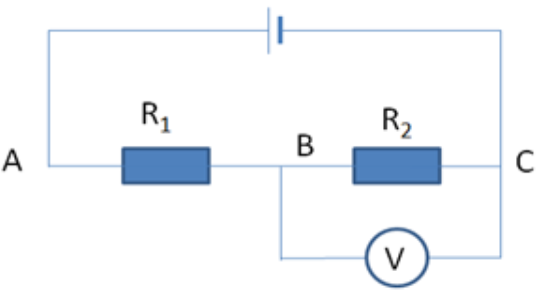
\includegraphics[scale=0.6]{../figs/VN11-2021-PH-TP014-3}
		\end{center}
			
			Mạch gồm $R_1$ nối tiếp ($R_2$ song song $R_V$). Khi đó:
			$$R=R_1 + R_{2V} = \SI{100}{\Omega} + \dfrac{500 R_V}{500 + R_V}.$$
			
			Cường độ dòng điện qua mạch:
			$$I=\dfrac{\calE}{R+r} \Rightarrow U_V = I R_{2V} = \SI{160}{V} \Rightarrow R_V = \SI{2051}{\Omega}.$$
			
		\item Khi Vôn kế mắc song song với $R_1$:
		\begin{center}
			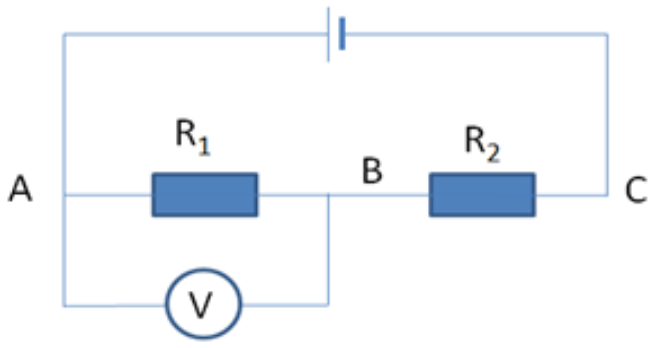
\includegraphics[scale=0.5]{../figs/VN11-2021-PH-TP014-4}
		\end{center}
	
		Mạch gồm $R_2$ nối tiếp ($R_1$ song song $R_V$). Khi đó:
		$$R'=R_2 + R_{1V} = \SI{595.45}{\Omega}.$$
		
		Cường độ dòng điện trong mạch:
		$$I' = \dfrac{\calE}{R' + r} = \SI{0.336}{A}.$$
		
		Số chỉ Vôn kế khi đó:
		$$U_V = I R_{1V} = \SI{32.04}{V}.$$
		\end{itemize}
	}
	\item \mkstar{4}
	
	\cauhoi{
		Cho mạch điện như hình vẽ.
		\begin{center}
			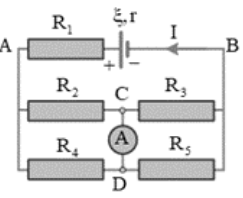
\includegraphics{../figs/VN11-2021-PH-TP014-1-2-3}
		\end{center}
	Cho biết $\calE = \SI{6}{V}$, $r=\SI{0.5}{\Omega}$, $R_1 = R_2 = \SI{2}{\Omega}$, $R_3=R_5 = \SI{4}{\Omega}$, $R_4=\SI{6}{\Omega}$. Điện trở của Ampe kế và dây nối không đáng kể. Tìm số chỉ của Ampe kế.
	}
	
	\loigiai{
		
		Mạch ngoài gồm: $R_1$ nối tiếp ($R_2$ song song $R_4$) nối tiếp ($R_3$ song song $R_5$).
		
		Tính: $R_{24} = \SI{1.5}{\Omega}$, $R_{35} = \SI{2}{\Omega}$. Suy ra $R=R_1 + R_{24} + R_{35} = \SI{5.5}{\Omega}$. Suy ra:
		$$I=\dfrac{\calE}{R+r} = \SI{1}{A}.$$
		
		Tính: $U_{24} = U_2 = I_2 R_2$, suy ra:
		$$I_2 = I \dfrac{R_{24}}{R_2} = \SI{0.75}{A}.$$
		
		Tính $U_{35} = U_3 = I_3 R_3$, suy ra:
		$$I_3 = I \dfrac{R_{35}}{R_3} = \SI{0.5}{A}.$$
		
		Do $I_2 > I_3$ nên $I_A = I_2 - I_3 = \SI{0.25}{A}$.
	}
	
\end{enumerate}
\stopcontents[mychapters]
\setcounter{mychapter}{9}
\mychapter{Ghép các nguồn điện thành bộ}
\startcontents[mychapters]
\printcontents[mychapters]{}{0}{\setcounter{tocdepth}{1}}
\whiteBGstarBegin
\setcounter{section}{0}
\section{Trắc nghiệm}
\begin{enumerate}[label=\bfseries Câu \arabic*:]
	
	
	\item \mkstar{1}
	
	\cauhoi
	{Việc ghép nối tiếp các nguồn điện thì sẽ tạo thành một bộ nguồn mới có
		\begin{mcq}
			\item suất điện động lớn hơn các nguồn có sẵn.
			\item suất điện động nhỏ hơn các nguồn có sẵn.
			\item điện trở trong nhỏ hơn các nguồn có sẵn.
			\item điện trở trong bằng điện trở ngoài.
		\end{mcq}
		
	}
	\loigiai
	{	\textbf{Đáp án: A.}
		
		Việc ghép nối tiếp các nguồn điện thì sẽ tạo thành một bộ nguồn mới có suất điện động lớn hơn các nguồn có sẵn.
		$$\calE = \calE_1 + \calE_2 + \ldots + \calE_n.$$
	}
	\item \mkstar{1}
	
	\cauhoi
	{Việc ghép song song các nguồn điện giống nhau thì sẽ tạo thành một bộ nguồn mới có
		\begin{mcq}
		\item suất điện động lớn hơn các nguồn có sẵn.
		\item suất điện động nhỏ hơn các nguồn có sẵn.
		\item điện trở trong nhỏ hơn các nguồn có sẵn.
		\item điện trở trong bằng điện trở ngoài.
		\end{mcq}
		
	}
	\loigiai
	{	\textbf{Đáp án: C.}
		
		Việc ghép song song các nguồn điện giống nhau thì sẽ tạo thành một bộ nguồn mới có điện trở trong nhỏ hơn các nguồn có sẵn.
		$$r=\dfrac{r_1 r_2 \ldots r_n}{r_1 + r_2 + \ldots + r_n} = \dfrac{r^n}{nr}.$$
	}
	\item \mkstar{2}
	
	\cauhoi
	{Ghép nối tiếp 3 pin giống nhau, mỗi pin có suất điện động 2 V và điện trở trong $\SI{1}{\Omega}$. Suất điện động và điện trở trong của bộ pin là
		\begin{mcq}(2)
			\item $\calE = \SI{6}{V}$ và $r=\SI{3}{\Omega}$.
			\item $\calE = \SI{9}{V}$ và $r=\xsi{1/3}{\Omega}$.
			\item $\calE = \SI{3}{V}$ và $r=\SI{3}{\Omega}$.
			\item $\calE = \SI{3}{V}$ và $r=\xsi{1/3}{\Omega}$.
		\end{mcq}
		
	}
	\loigiai
	{	\textbf{Đáp án: A.}
		
		Khi ghép nối tiếp bộ nguồn thì:
		
		Suất điện động của bộ nguồn:
		$$\calE_\text b= n \calE = \SI{6}{V}.$$
		
		Điện trở trong của bộ nguồn:
		$$r_\text b = nr = \SI{3}{\Omega}.$$
	}
	\item \mkstar{2}
	
	\cauhoi
	{Một mạch điện kín gồm hai nguồn điện $\calE_1$, $r_1$ và $\calE_2$, $r_2$ mắc nối tiếp nhau. Mạch ngoài chỉ có điện trở $R$. Biểu thức cường độ dòng điện trong mạch ngoài là
		\begin{mcq}(2)
			\item $I=\dfrac{\calE_1 - \calE_2}{R+r_1+r_2}$.
			\item $I=\dfrac{\calE_1 - \calE_2}{R+r_1-r_2}$.
			\item $I=\dfrac{\calE_1 + \calE_2}{R+r_1-r_2}$.
			\item $I=\dfrac{\calE_1 + \calE_2}{R+r_1+r_2}$.
		\end{mcq}
		
	}
	\loigiai
	{	\textbf{Đáp án: D.}
		
		Một mạch điện kín gồm hai nguồn điện $\calE_1$, $r_1$ và $\calE_2$, $r_2$ mắc nối tiếp nhau. Biểu thức cường độ dòng điện trong mạch:
		$$I=\dfrac{\calE_1 + \calE_2}{R + r_1 + r_2}.$$
	}
	\item \mkstar{2}
	
	\cauhoi
	{Một mạch điện kín gồm hai nguồn điện $\calE$, $r_1$ và $\calE$, $r_2$ mắc song song với nhau. Mạch ngoài chỉ có điện trở $R$. Biểu thức cường độ dòng điện trong mạch là
		\begin{mcq}(2)
			\item $I=\dfrac{2\calE}{R+r_1+r_2}$.
			\item $I=\dfrac{\calE}{R+\dfrac{r_1 r_2}{r_1 + r_2}}$.
			\item $I=\dfrac{2\calE}{R+\dfrac{r_1 r_2}{r_1 + r_2}}$.
			\item $I=\dfrac{\calE}{R+\dfrac{r_1+r_2}{r_1 r_2}}$.
		\end{mcq}
		
	}
	\loigiai
	{	\textbf{Đáp án: B.}
		
		Một mạch điện kín gồm hai nguồn điện $\calE$, $r_1$ và $\calE$, $r_2$ mắc song song với nhau, mạch ngoài chỉ có điện trở $R$. Biểu thức cường độ dòng điện trong mạch là
		$$I=\dfrac{\calE}{R + \dfrac{r_1 r_2}{r_1 + r_2}}.$$
	}
	\item \mkstar{2}
	
	\cauhoi
	{Một bộ nguồn gồm hai nguồn điện mắc nối tiếp. Hai nguồn có suất điện động lần lượt là 5 V và 7 V. Suất điện động của bộ nguồn là
		\begin{mcq}(4)
			\item 6 V.
			\item 2 V.
			\item 12 V.
			\item 7 V.
		\end{mcq}
		
	}
	\loigiai
	{	\textbf{Đáp án: C.}
		
		Suất điện động của bộ nguồn mắc nối tiếp:
		$$\calE = \calE_1 + \calE_2 = \SI{12}{V}.$$
	}
	\item \mkstar{2}
	
	\cauhoi
	{Khi ghép $n$ nguồn điện nối tiếp, mỗi nguồn có suất điện động $\calE$ và điện trở trong $r$ thì suất điện động và điện trở trong của bộ nguồn là
		\begin{mcq}(2)
			\item $n\calE$ và $nr$.
			\item $\calE$ và $\dfrac{r}{n}$.
			\item $n\calE$ và $\dfrac{\calE}{n}$.
			\item $\calE$ và $nr$.
		\end{mcq}
		
	}
	\loigiai
	{	\textbf{Đáp án: A.}
		
		Suất điện động của bộ nguồn mắc nối tiếp: $n \calE$.
		
		Điện trở trong của bộ nguồn mắc nối tiếp: $nr$.
	}
	\item \mkstar{2}
	
	\cauhoi
	{Nguồn điện với suất điện động $\calE$, điện trở trong $r$, mắc với điện trở ngoài $R=r$, cường độ dòng điện trong mạch là $I$. Nếu thay nguồn điện đó bằng 3 nguồn điện giống hệt nó mắc nối tiếp thì cường độ dòng điện trong mạch là
		\begin{mcq}(2)
			\item $I'=3I$.
			\item $I'=2I$.
			\item $I'=\SI{2.5}{}I$.
			\item $I'=\SI{1.5}{}I$.
		\end{mcq}
		
	}
	\loigiai
	{	\textbf{Đáp án: D.}
		
		Cường độ dòng điện lúc đầu:
		$$I=\dfrac{\calE}{R+r} = \dfrac{\calE}{2r}.$$
		
		Cường độ dòng điện lúc sau:
		$$I' = \dfrac{3\calE}{R + 3r} = \dfrac{3\calE}{4r}.$$
		
		Lập tỉ lệ:
		$$\dfrac{I}{I'} = \dfrac{2}{3} \Rightarrow I' = \SI{1.5}{} I.$$
	}
	\item \mkstar{2}
	
	\cauhoi
	{Cho bộ nguồn gồm 6 ắcquy giống nhau được mắc thành hai dãy song song, mỗi dãy gồm 3 ắcquy ghép nối tiếp. Mỗi ắcquy có suất điện động $\calE = \SI{2}{V}$ và điện trở trong $r=\SI{1}{\Omega}$. Suất điện động và điện trở trong của bộ nguồn lần lượt là
		\begin{mcq}(2)
			\item $\calE_\text{b} = \SI{12}{V}$, $r_\text{b} = \SI{6}{\Omega}$.
			\item $\calE_\text{b} = \SI{6}{V}$, $r_\text{b} = \SI{3}{\Omega}$.
			\item $\calE_\text{b} = \SI{6}{V}$, $r_\text{b} = \SI{1.5}{\Omega}$.
			\item $\calE_\text{b} = \SI{12}{V}$, $r_\text{b} = \SI{3}{\Omega}$.
		\end{mcq}
		
	}
	\loigiai
	{	\textbf{Đáp án: C.}
		
		Suất điện động trên mỗi nhánh cũng là suất điện động của bộ nguồn:
		$$\calE_\text b = 3 \calE = \SI{6}{V}.$$
		
		Điện trở trong trên mỗi nhánh:
		$$3r = \SI{3}{\Omega}.$$
		
		Điện trở trong của bộ nguồn:
		$$r_\text{b} = \dfrac{\SI{3}{\Omega}}{2} = \SI{1.5}{\Omega}.$$
	}
	\item \mkstar{2}
	
	\cauhoi
	{Cho bộ nguồn gồm 6 ắcquy giống nhau được mắc thành ba dãy song song, mỗi dãy gồm 2 ắcquy ghép nối tiếp. Mỗi ắcquy có suất điện động $\calE = \SI{2}{V}$ và điện trở trong $r=\SI{1.5}{\Omega}$. Suất điện động và điện trở trong của bộ nguồn lần lượt là
		\begin{mcq}(2)
			\item $\calE_\text{b} = \SI{12}{V}$, $r_\text{b} = \SI{6}{\Omega}$.
			\item $\calE_\text{b} = \SI{6}{V}$, $r_\text{b} = \SI{1}{\Omega}$.
			\item $\calE_\text{b} = \SI{4}{V}$, $r_\text{b} = \SI{1.5}{\Omega}$.
			\item $\calE_\text{b} = \SI{4}{V}$, $r_\text{b} = \SI{1}{\Omega}$.
		\end{mcq}
		
	}
	\loigiai
	{	\textbf{Đáp án: D.}
		
		Suất điện động trên mỗi nhánh cũng là suất điện động của bộ nguồn:
		$$\calE_\text b = 2\calE = \SI{4}{V}.$$
		
		Điện trở trong trên mỗi nhánh:
		$$2r = \SI{3}{\Omega}.$$
		
		Điện trở trong của bộ nguồn:
		$$r_\text{b} = \dfrac{\SI{3}{\Omega}}{3} = \SI{1}{\Omega}.$$
	}
	\item \mkstar{2}
	
	\cauhoi
	{Người ta mắc một bộ 3 pin giống nhau song song thì thu được một bộ nguồn có suất điện động 9 V và điện trở trong $\SI{3}{\Omega}$. Mỗi pin có suất điện động và điện trở trong lần lượt là
		\begin{mcq}(2)
			\item $\calE = \SI{9}{V}$, $r=\SI{3}{\Omega}$.
			\item $\calE=\SI{9}{V}$, $r=\SI{9}{\Omega}$.
			\item $\calE=\SI{27}{V}$, $r=\SI{9}{\Omega}$.
			\item $\calE=\SI{3}{V}$, $r=\SI{3}{\Omega}$.
		\end{mcq}
		
	}
	\loigiai
	{	\textbf{Đáp án: B.}
		
		Suất điện động của mỗi nguồn cũng là suất điện động của bộ nguồn:
		$$\calE = \calE_\text b = \SI{9}{V}.$$
		
		Điện trở trong của mỗi nguồn:
		$$r_\text{b} = \dfrac{r}{3} \Rightarrow r=\SI{9}{\Omega}.$$
	}
	\item \mkstar{2}
	
	\cauhoi
	{Người ta mắc một bộ 3 pin giống nhau nối tiếp thì thu được một bộ nguồn có suất điện động 9 V và điện trở trong $\SI{3}{\Omega}$. Mỗi pin có suất điện động và điện trở trong lần lượt là
		\begin{mcq}(2)
			\item $\calE = \SI{9}{V}$, $r=\SI{1}{\Omega}$.
			\item $\calE=\SI{9}{V}$, $r=\SI{9}{\Omega}$.
			\item $\calE=\SI{3}{V}$, $r=\SI{3}{\Omega}$.
			\item $\calE=\SI{3}{V}$, $r=\SI{1}{\Omega}$.
		\end{mcq}
		
	}
	\loigiai
	{	\textbf{Đáp án: D.}
		
		Suất điện động của mỗi nguồn:
		$$\calE_\text{b} = 3\calE \Rightarrow \calE = \SI{3}{V}.$$
		
		Điện trở trong của mỗi nguồn:
		$$r_\text{b} = 3r \Rightarrow r = \SI{1}{\Omega}.$$
	}
	\item \mkstar{2}
	
	\cauhoi
	{Nếu ghép 3 pin giống nhau nối tiếp thì được bộ nguồn có suất điện động $\SI{7.5}{V}$ và điện trở trong $\SI{3}{\Omega}$. Nếu ghép 3 pin đó song song thì thu được bộ nguồn có suất điện động và điện trở trong lần lượt là
		\begin{mcq}(2)
			\item $\SI{7.5}{V}$ và $\SI{1}{\Omega}$.
			\item $\SI{7.5}{V}$ và $\SI{3}{\Omega}$.
			\item $\SI{2.5}{V}$ và $\xsi{1/3}{\Omega}$.
			\item $\SI{2.5}{V}$ và $\SI{1}{\Omega}$.
		\end{mcq}
		
	}
	\loigiai
	{	\textbf{Đáp án: C.}
		
		Suất điện động của mỗi pin:
		$$\calE = \SI{2.5}{V}.$$
		
		Điện trở trong của mỗi pin:
		$$r=\SI{1}{\Omega}.$$
		
		Suất điện động của bộ nguồn ghép song song:
		$$\calE_\text b = \calE = \SI{2.5}{V}.$$
		
		Điện trở trong của bộ nguồn ghép song song:
		$$r_\text{b} = \dfrac{r}{3} = \xsi{\dfrac{1}{3}}{\Omega}.$$
	}
	\item \mkstar{2}
	
	\cauhoi
	{Cho 4 pin giống nhau loại $\SI{1.5}{V}$, khi ghép chúng lại với nhau, ta có thể thu được bộ nguồn có suất điện động nào dưới đây?
		\begin{mcq}(4)
			\item 1 V.
			\item 3 V.
			\item 2 V.
			\item 4 V.
		\end{mcq}
		
	}
	\loigiai
	{	\textbf{Đáp án: B.}
		
		Cách để ghép thành bộ nguồn có suất điện động $\SI{3}{V}$ là ghép song song bộ nguồn thành 2 nhánh, mỗi nhánh có 2 pin nối tiếp.
	}
	\item \mkstar{2}
	
	\cauhoi
	{Cho 3 pin giống nhau loại $\SI{1.5}{V}$, khi ghép chúng lại với nhau, ta \textbf{không} thể thu được bộ nguồn có suất điện động nào dưới đây?
		\begin{mcq}(4)
			\item $\SI{4.5}{V}$.
			\item $\SI{1.5}{V}$.
			\item $\SI{1}{V}$.
			\item $\SI{3}{V}$.
		\end{mcq}
		
	}
	\loigiai
	{	\textbf{Đáp án: C.}
		
		Cách để ghép thành bộ nguồn có suất điện động $\SI{4.5}{V}$ là nối tiếp 3 pin.
		
		Cách để ghép thành bộ nguồn có suất điện động $\SI{1.5}{V}$ là song song 3 pin.
		
		Cách để ghép thành bộ nguồn có suất điện động $\SI{3}{V}$ là (1 pin) nối tiếp với (2 pin song song).
		
		Không có cách nào để ghép thành bộ nguồn có suất điện động $\SI{1}{V}$.
	}
	\item \mkstar{3}
	
	\cauhoi
	{Cho mạch điện như hình vẽ.
		\begin{center}
			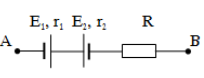
\includegraphics{../figs/VN11-2021-PH-TP015-1}
		\end{center}
	Trong đó: $\calE_1 = \SI{9}{V}$, $r_1=\SI{1.2}{\Omega}$, $\calE_2 = \SI{3}{V}$, $r_2=\SI{0.4}{\Omega}$, $R=\SI{28.4}{\Omega}$. Hiệu điện thế giữa hai đầu mạch là $U_\text{AB} = \SI{6}{V}$. Xác định chiều và độ lớn của cường độ dòng điện trong mạch.
		\begin{mcq}
			\item Chiều từ A sang B, độ lớn $I=\SI{0.4}{A}$.
			\item Chiều từ B sang A, độ lớn $I=\SI{0.4}{A}$.
			\item Chiều từ A sang B, độ lớn $I=\SI{0.6}{A}$.
			\item Chiều từ B sang A, độ lớn $I=\SI{0.6}{A}$.
		\end{mcq}
		
	}
	\loigiai
	{	\textbf{Đáp án: A.}
		
		Vì $\calE_1$ và $\calE_2$ mắc ngược chiều, mà $\calE_1 > \calE_2$ nên $\calE_1$ là nguồn, $\calE_2$ là máy thu. Do đó chiều dòng điện theo chiều từ A sang B.
		
		Cường độ dòng điện trong mạch:
		$$I=\dfrac{U_\text{AB} + \calE_1 - \calE_2}{R + r_1 + r_2} = \SI{0.4}{A}.$$
	}
	\item \mkstar{3}
	
	\cauhoi
	{Hai nguồn điện giống nhau, mỗi nguồn có suất điện động là 2 V, điện trở trong là $\SI{1}{\Omega}$, được mắc song song với nhau và nối với một điện trở ngoài $R$. Điện trở $R$ bằng bao nhiêu để cường độ dòng điện đi qua nó là 1 A?
		\begin{mcq}(4)
			\item $\SI{1.5}{\Omega}$.
			\item $\SI{1}{\Omega}$.
			\item $\SI{2}{\Omega}$.
			\item $\SI{3}{\Omega}$.
		\end{mcq}
		
	}
	\loigiai
	{	\textbf{Đáp án: A.}
		
		Suất điện động của nguồn:
		$$\calE_\text b = \calE = \SI{2}{V}.$$
		
		Điện trở trong của nguồn:
		$$r_\text b= \dfrac{r}{2} = \SI{0.5}{\Omega}$$
		
		Cường độ dòng điện đi qua $R$ là
		$$I=\dfrac{\calE_\text b}{R+r_\text b} = 1 \Rightarrow R = \SI{1.5}{\Omega}.$$
	}
	\item \mkstar{3}
	
	\cauhoi
	{Có 8 nguồn điện cùng loại với cùng suất điện động $\calE=\SI{2}{V}$ và điện trở trong $r=\SI{1}{\Omega}$. Mắc các nguồn thành bộ hỗn hợp đối xứng gồm hai dãy song song. Suất điện động $\calE_\text{b}$ và điện trở trong $r_\text{b}$ của bộ này bằng
		\begin{mcq}(2)
			\item $\calE_\text{b} = \SI{4}{V}$ và $r_\text{b} = \SI{2}{\Omega}$.
			\item $\calE_\text{b} = \SI{6}{V}$ và $r_\text{b} = \SI{4}{\Omega}$.
			\item $\calE_\text{b} = \SI{6}{V}$ và $r_\text{b} = \SI{1}{\Omega}$.
			\item $\calE_\text{b} = \SI{8}{V}$ và $r_\text{b} = \SI{2}{\Omega}$.
		\end{mcq}
		
	}
	\loigiai
	{	\textbf{Đáp án: D.}
		
		Suất điện động của bộ nguồn:
		$$\calE_\text b = 4 \calE = \SI{8}{V}.$$
		
		Điện trở trong của bộ nguồn:
		$$r_\text b = \dfrac{4r}{2} = 2r =\SI{2}{\Omega}.$$
	}
	\item \mkstar{3}
	
	\cauhoi
	{Có 24 nguồn điện giống nhau, suất điện động và điện trở trong của mỗi nguồn là $\calE=\SI{1.5}{V}$ và $r=\SI{0.5}{\Omega}$, mắc hỗn hợp đối xứng thành bốn dãy song song với nhau (mỗi dãy có 6 nguồn điện mắc nối tiếp). Suất điện động và điện trở trong của bộ nguồn này là
		\begin{mcq}(2)
			\item 6 V và $\SI{0.75}{\Omega}$.
			\item 9 V và $\SI{1.5}{\Omega}$.
			\item 6 V và $\SI{1.5}{\Omega}$.
			\item 9 V và $\SI{0.75}{\Omega}$.
		\end{mcq}
		
	}
	\loigiai
	{	\textbf{Đáp án: D.}
		
		Mắc 4 dãy, mỗi dãy có 6 nguồn nối tiếp:
		$$\calE_\text = 6\calE = \SI{9}{V}.$$
		$$r_\text b = \dfrac{6r}{4} = \SI{0.75}{\Omega}.$$
	}
	\item \mkstar{4}
	
	\cauhoi
	{Cho mạch điện như hình vẽ.
		\begin{center}
			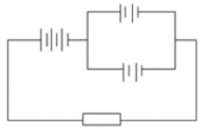
\includegraphics{../figs/VN11-2021-PH-TP015-2.png}
		\end{center}
	Mỗi pin có suất điện động $\calE=\SI{1.5}{V}$, $r=\SI{1}{\Omega}$, $R=\SI{3.5}{\Omega}$. Tìm cường độ dòng điện mạch ngoài.
		\begin{mcq}(4)
			\item $\SI{0.5}{A}$.
			\item 1 A.
			\item 2 A.
			\item $\SI{1.5}{A}$.
		\end{mcq}
		
	}
	\loigiai
	{	\textbf{Đáp án: B.}
		
		Xét đoạn mạch gồm 2 nhánh song song, mỗi nhánh gồm 2 nguồn nối tiếp thì ta có
		$$\calE_\text{ss} = 2 \calE;\ r_\text{ss} = \dfrac{2r}{2} = \SI{1}{\Omega}.$$
		
		Đoạn mạch gồm 3 nguồn nối tiếp thì ta có
		$$\calE_\text{nt} = 3 \calE = \SI{4.5}{V};\ r_\text{nt} = 3r = \SI{3}{\Omega}.$$
		$$\Rightarrow \calE = \calE_\text{ss} + \calE_\text{nt} = \SI{7.5}{V};\ r_\text{b} = r_\text{ss} + r_\text{nt} = \SI{4}{\Omega}.$$
		
		Cường độ dòng điện mạch ngoài là
		$$I=\dfrac{\calE_\text b}{R+ r_\text b} = \SI{1}{A}.$$
	}
\end{enumerate}

\whiteBGstarEnd

\loigiai
{
	\begin{center}
		\textbf{BẢNG ĐÁP ÁN}
	\end{center}
	\begin{center}
		\begin{tabular}{|m{2.8em}|m{2.8em}|m{2.8em}|m{2.8em}|m{2.8em}|m{2.8em}|m{2.8em}|m{2.8em}|m{2.8em}|m{2.8em}|}
			\hline
			1.A  & 2.C  & 3.A  & 4.D  & 5.B  & 6.C  & 7.A  & 8.D  & 9.C  & 10.D  \\
			\hline
			11.B  & 12.D  & 13.C  & 14.B  & 15.C  & 16.A  & 17.A  & 18.D  & 19.D  & 20.B  \\
			\hline
		\end{tabular}
	\end{center}
}
\section{Tự luận}
\begin{enumerate}[label=\bfseries Câu \arabic*:]
	\item \mkstar{1}
	
	\cauhoi{
		Dòng điện chạy qua đoạn mạch chứa nguồn điện có chiều như thế nào? Hãy trình bày các mối quan hệ trong đoạn mạch có chứa nguồn điện.
	}
	
	\loigiai{
		
		Dòng điện chạy qua đoạn mạch chứa nguồn điện có chiều đi ra từ cực dương và đi tới cực âm của nguồn điện.
		\begin{center}
			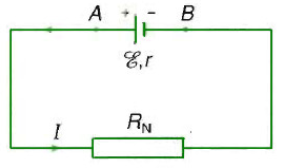
\includegraphics[scale=1]{../figs/VN11-2021-PH-TP015-3}
		\end{center}
	
		Trong đoạn mạch có chứa nguồn điện, mối quan hệ giữa các đại lượng được biểu diễn bằng công thức:
		$$U_\text{AB} = \calE - Ir,$$
		trong đó:
		\begin{itemize}
			\item $r$ là điện trở trong của nguồn điện;
			\item $\calE$ là suất điện động của nguồn điện.
		\end{itemize}
	}
	
	\item \mkstar{2}
	
	\cauhoi{
		Một bộ nguồn gồm hai nguồn điện mắc nối tiếp. Hai nguồn điện có suất điện động lần lượt là 5 V và 7 V. Tìm suất điện động của bộ nguồn.
	}
	
	\loigiai{
		
		Vì bộ nguồn mắc nối tiếp nên suất điện động của bộ nguồn là
		$$\calE = \calE_1 + \calE_2 = \SI{12}{V}.$$
	}
	\item \mkstar{3}
	
	\cauhoi{
		Một ắcquy có suất điện động và điện trở trong $\calE=\SI{6}{V}$ và $r=\SI{0.6}{\Omega}$. Sử dụng ắcquy này thắp sáng bóng đèn có ghi 6 V - 3 W. Tính cường độ dòng điện chạy trong mạch và hiệu điện thế giữa hai cực của ắcquy đó.
	}
	
	\loigiai{
		
		Điện trở của bóng đèn:
		$$R_\text{đ} = \dfrac{U_\text{đm}^2}{\calP_\text{đm}} = \SI{12}{\Omega}.$$
		
		Cường độ dòng điện chạy trong mạch:
		$$I=\dfrac{\calE}{R_\text{đ} + r} = \SI{0.476}{A}.$$
		
		Hiệu điện thế giữa hai cực của ắc quy khi đó:
		$$U=\calE - Ir = \SI{5.714}{V}.$$
	}
	\item \mkstar{4}
	
	\cauhoi{
		Cần dùng bao nhiêu pin $\SI{4.5}{V}$ - $\SI{1}{\Omega}$ mắc theo kiểu hỗn hợp để thắp cho bóng đèn 8 V - 8 W sáng bình thường?
	}
	
	\loigiai{
		
		Điện trở của đèn:
		$$R=\dfrac{U^2}{\calP} = \SI{8}{\Omega}.$$
		
		Giả sử pin mắc thành n dãy song song, mỗi dãy có m nguồn ghép nối tiếp.
		
		Ta có cường độ dòng điện đi qua mạch để đèn sáng bình thường là
		$$I=\dfrac{\calP}{U} = \SI{1}{A}.$$
		
		Suy ra:
		$$I=\dfrac{\calE_\text b}{R + r_\text b} = \dfrac{m \calE}{8 + \dfrac{mr}{n}} = \dfrac{4,5 mn}{m+8n} = \dfrac{4,5 p}{m+8n}\ (1).$$
		
		Thay $n=\dfrac{p}{m}$ vào (1) ta có:
		$$p=\dfrac{m^2}{4,5m - 8}.$$
		
		Vì $p$ dương nên $m> \dfrac{16}{9}$ hay $m>1$.
		$$n=\dfrac{p}{m} \geq 1 \Leftrightarrow \dfrac{m^2}{4,5m - 8} \geq 1 \Rightarrow m \leq 2,3$$
		
		Suy ra $m=2$, $n=2$ (có 4 pin được mắc thành 2 nhánh song song, mỗi nhánh gồm 2 pin nối tiếp).
	}
	\item \mkstar{4}
	
	\cauhoi{
		Một nguồn điện có suất điện động $\calE=\SI{1.5}{\Omega}$, điện trở trong $r=\SI{0.1}{\Omega}$. Mắc với hai cực của nguồn điện trở $R_1$ và $R_2$ thành mạch kín. Khi $R_1$ nối tiếp $R_2$ thì cường độ dòng điện qua mỗi điện trở là $\SI{1.5}{A}$. Khi $R_1$ song song $R_2$ thì cường độ dòng điện tổng cộng qua 2 điện trở là 5 A. Tìm giá trị của $R_1$ và $R_2$.
	}
	
	\loigiai{
		
		Khi $R_1$ nối tiếp $R_2$ thì cường độ dòng điện qua mỗi điện trở là
		$$I=\dfrac{\calE}{R_1 + R_2 + r}  \Rightarrow R_1 + R_2 = \SI{0.9}{\Omega}\ (*).$$
		
		Khi $R_1$ nối tiếp $R_2$ thì cường độ dòng điện tổng cộng qua 2 điện trở là
		$$I=\dfrac{\calE}{\dfrac{R_1 R_2}{R_1 + R_2} + r} \Rightarrow \dfrac{R_1 R_2}{R_1 + R_2} = \SI{0.2}{\Omega}\ (**).$$
		
		Từ $(*)$ và $(**)$, ta tính được:
		$$R_1 = \SI{0.6}{\Omega};\ R_2 = \SI{0.3}{\Omega}.$$
	}
	
\end{enumerate}
\stopcontents[mychapters]
\setcounter{mychapter}{10}
\mychapter{Phương pháp giải một số bài toán về toàn mạch}
\startcontents[mychapters]
\printcontents[mychapters]{}{0}{\setcounter{tocdepth}{1}}
\whiteBGstarBegin
\setcounter{section}{0}
\section{Trắc nghiệm}
\begin{enumerate}[label=\bfseries Câu \arabic*:]
	
	
	\item \mkstar{1}
	
	\cauhoi
	{Trong một mạch kín gồm nguồn điện có suất điện động $\calE$, điện trở trong $r$ và mạch ngoài có điện trở $R$. Hệ thức nêu lên mỗi quan hệ giữa các đại lượng trên với cường độ dòng điện $I$ chạy trong mạch là
		\begin{mcq}(4)
			\item $I=\dfrac{\calE}{R}$.
			\item $I=\calE \sqrt{\dfrac{\calE}{R}}$.
			\item $I=\dfrac{\calE}{R+r}$.
			\item $I=\dfrac{\calE}{r}$.
		\end{mcq}
		
	}
	\loigiai
	{	\textbf{Đáp án: C.}
		
		Định luật Ôm đối với toàn mạch: Cường độ dòng điện chạy trong mạch điện kín tỉ lệ thuận với suất điện động cua nguồn điện và tỉ lệ nghịch với điện trở toàn phần của mạch đó:
		$$I=\dfrac{\calE}{R+r},$$
		với $R$ là điện trở mạch ngoài; $r$ là điện trở trong của nguồn điện.
	}
	\item \mkstar{1}
	
	\cauhoi
	{Trong mạch điện kín gồm nguồn điện có suất điện động $\calE$, điện trở trong $r$ và mạch ngoài có điện trở $R$. Khi có hiện tượng đoản mạch thì cường độ dòng điện trong mạch $I$ được xác định bằng công thức:
		\begin{mcq}(4)
			\item $I=\dfrac{\calE}{r}$.
			\item $I=\calE r$.
			\item $I=\dfrac{r}{\calE}$.
			\item $I=\dfrac{\calE}{R+r}$.
		\end{mcq}
		
	}
	\loigiai
	{	\textbf{Đáp án: A.}
		
		Định luật Ôm đối với toàn mạch:
		$$I=\dfrac{\calE}{R+r}.$$
		
		Khi có hiện tượng đoản mạch ($R=0$) thì cường độ dòng điện trong mạch là
		$$I=\dfrac{\calE}{r}.$$
	}
	\item \mkstar{2}
	
	\cauhoi
	{Một điện trở $\SI{4}{\Omega}$ được mắc vào nguồn điện có suất điện động $\calE = \SI{1.5}{V}$ để tạo thành một mạch điện kín thì công suất tỏa nhiệt trên điện trở này bằng $\SI{0.36}{W}$. Hiệu điện thế giữa hai đầu điện trở $R$ là
		\begin{mcq}(4)
			\item 1 V.
			\item $\SI{1.2}{V}$.
			\item $\SI{1.4}{V}$.
			\item $\SI{1.6}{V}$.
		\end{mcq}
		
	}
	\loigiai
	{	\textbf{Đáp án: B.}
		
		Hiệu điện thế giữa hai đầu điện trở:
		$$\calP = \dfrac{U^2}{R} \Rightarrow U=\SI{1.2}{V}.$$
	}
	\item \mkstar{2}
	
	\cauhoi
	{Một điện trở $\SI{4}{\Omega}$ được mắc vào nguồn điện có suất điện động $\calE = \SI{1.5}{V}$ để tạo thành một mạch điện kín thì công suất tỏa nhiệt trên điện trở này bằng $\SI{0.36}{W}$. Điện trở trong của nguồn điện là
		\begin{mcq}(4)
			\item $\SI{0.5}{\Omega}$.
			\item $\SI{0.25}{\Omega}$.
			\item $\SI{5}{\Omega}$.
			\item $\SI{1}{\Omega}$.
		\end{mcq}
		
	}
	\loigiai
	{	\textbf{Đáp án: D.}
		
		Hiệu điện thế giữa hai đầu điện trở:
		$$\calP = \dfrac{U^2}{R} \Rightarrow U=\SI{1.2}{V}.$$
		
		Cường độ dòng điện chạy trong mạch:
		$$\calP = UI \Rightarrow I=\SI{0.3}{A}.$$
		
		Áp dụng định luật Ôm toàn mạch:
		$$I=\dfrac{\calE}{R+r} \Rightarrow r = \SI{1}{\Omega}.$$
	}
	\item \mkstar{2}
	
	\cauhoi
	{Hai bóng đèn có điện trở $\SI{5}{\Omega}$ mắc song song với nhau và nối vào một nguồn điện có điện trở trong $\SI{1}{\Omega}$ thì cường độ dòng điện trong mạch là $\xsi{12/7}{A}$. Khi tháo một bóng đèn ra thì cường độ dòng điện trong mạch là
		\begin{mcq}(4)
			\item $\xsi{6/5}{A}$.
			\item 1 A.
			\item $\xsi{5/6}{A}$.
			\item 0 A.
		\end{mcq}
		
	}
	\loigiai
	{	\textbf{Đáp án: B.}
		
		Áp dụng định luật Ôm toàn mạch:
		$$I=\dfrac{\calE}{r + \dfrac{R R}{R + R}} \Rightarrow \calE = \SI{6}{V}.$$
		
		Khi tháo một bóng đèn ra, áp dụng định luật Ôm toàn mạch:
		$$I' = \dfrac{\calE}{r + R} = \SI{1}{A}.$$
	}
	\item \mkstar{2}
	
	\cauhoi
	{Cho đoạn mạch gồm điện trở $R_1=\SI{100}{\Omega}$ mắc nối tiếp với điện trở $R_2=\SI{200}{\Omega}$, hiệu điện thế giữa hai đầu đoạn mạch là $\SI{12}{V}$. Hiệu điện thế giữa hai đầu điện trở $R_1$ là
		\begin{mcq}(4)
			\item $U_1 = \SI{1}{V}$.
			\item $U_1=\SI{8}{V}$.
			\item $U_1=\SI{4}{V}$.
			\item $U_1=\SI{6}{V}$.
		\end{mcq}
		
	}
	\loigiai
	{	\textbf{Đáp án: C.}
		
		Cường độ dòng điện qua mạch:
		$$I=\dfrac{U}{R} = \dfrac{U}{R_1 + R_2} = \SI{0.04}{A}.$$
		
		Hiệu điện thế giữa hai đầu $R_1$:
		$$U_1 = I R_1 = \SI{4}{V}.$$
	}
	\item \mkstar{2}
	
	\cauhoi
	{Cho đoạn mạch gồm điện trở $R_1=\SI{100}{\Omega}$ mắc nối tiếp với điện trở $R_2=\SI{200}{\Omega}$, hiệu điện thế giữa hai đầu đoạn mạch là $\SI{12}{V}$. Hiệu điện thế giữa hai đầu điện trở $R_2$ là
		\begin{mcq}(4)
			\item $U_1=\SI{1}{V}$.
			\item $U_1=\SI{8}{V}$.
			\item $U_1=\SI{4}{V}$.
			\item $U_1=\SI{6}{V}$.
		\end{mcq}
		
	}
	\loigiai
	{	\textbf{Đáp án: B.}
		
		Cường độ dòng điện qua mạch:
		$$I=\dfrac{U}{R} = \dfrac{U}{R_1 + R_2} = \SI{0.04}{A}.$$
		
		Hiệu điện thế giữa hai đầu $R_2$:
		$$U_2 = I R_2= \SI{8}{V}.$$
	}
	\item \mkstar{2}
	
	\cauhoi
	{Một nguồn điện có suất điện động $\calE = \SI{12}{V}$, điện trở trong $\SI{2}{\Omega}$ nối tiếp với điện trở $R$ tạo thành mạch điện kín. Công suất tiêu thụ trên điện trở $R$ bằng 16 W. Biết $R>\SI{2}{\Omega}$, giá trị của $R$ là
		\begin{mcq}(4)
			\item $\SI{3}{\Omega}$.
			\item $\SI{6}{\Omega}$.
			\item $\SI{5}{\Omega}$.
			\item $\SI{4}{\Omega}$.
		\end{mcq}
		
	}
	\loigiai
	{	\textbf{Đáp án: D.}
		
		Công suất tiêu thụ trên điện trở:
		$$\calP = I^2 R \Rightarrow \calP = \left(\dfrac{\calE}{R + r}\right)^2 R \Rightarrow R^2 + 2Rr + r^2 = \dfrac{\calE^2 R}{\calP}.$$
		
		Giải phương trình bậc hai trên, tính được $R=\SI{4}{\Omega}$ hoặc $R=\SI{1}{\Omega}$.
		
		Mà theo đề bài thì $R>\SI{2}{\Omega}$, nên giá trị $R$ là $R=\SI{4}{\Omega}$.
	}
	\item \mkstar{2}
	
	\cauhoi
	{Cho mạch điện gồm nguồn điện ($\calE=\SI{12}{V}$, $r=\SI{1}{\Omega}$) nối với mạch ngoài gồm 3 điện trở mắc nối tiếp: $R_1=\SI{3}{\Omega}$, $R_2=\SI{6}{\Omega}$, $R_3=\SI{5}{\Omega}$. Tính hiệu điện thế giữa hai đầu điện trở $R_2$.
		\begin{mcq}(4)
			\item $\SI{3.5}{V}$.
			\item $\SI{4.8}{V}$.
			\item $\SI{2.5}{V}$.
			\item $\SI{4.5}{V}$.
		\end{mcq}
		
	}
	\loigiai
	{	\textbf{Đáp án: B.}
		
		Cường độ dòng điện qua mạch:
		$$I=\dfrac{\calE}{R + r} = \dfrac{\calE}{R_1 + R_2 + R_3 + r} = \SI{0.8}{A}.$$
		
		Hiệu điện thế giữa hai đầu $R_2$:
		$$U_2 = I R_2 = \SI{4.8}{V}.$$
	}
	\item \mkstar{2}
	
	\cauhoi
	{Cho mạch điện gồm nguồn điện ($\calE=\SI{12}{V}$, $r=\SI{1}{\Omega}$) nối với mạch ngoài gồm 3 điện trở mắc nối tiếp: $R_1=\SI{3}{\Omega}$, $R_2=\SI{6}{\Omega}$, $R_3=\SI{5}{\Omega}$. Tính hiệu điện thế giữa hai đầu đoạn mạch.
		\begin{mcq}(4)
			\item $\SI{6.5}{V}$.
			\item $\SI{11.8}{V}$.
			\item $\SI{11.2}{V}$.
			\item $\SI{6.2}{V}$.
		\end{mcq}
		
	}
	\loigiai
	{	\textbf{Đáp án: C.}
		
		Cường độ dòng điện qua mạch:
		$$I=\dfrac{\calE}{R + r} = \dfrac{\calE}{R_1 + R_2 + R_3 + r} = \SI{0.8}{A}.$$
		
		Hiệu điện thế giữa hai đầu đoạn mạch:
		$$U=IR = \SI{11.2}{V}.$$
	}
	\item \mkstar{2}
	
	\cauhoi
	{Cho mạch điện gồm nguồn điện ($\calE=\SI{12}{V}$, $r=\SI{1}{\Omega}$) nối với mạch ngoài gồm 3 điện trở mắc song song: $R_1=\SI{3}{\Omega}$, $R_2=\SI{6}{\Omega}$, $R_3=\SI{5}{\Omega}$. Tính hiệu điện thế giữa hai đầu điện trở $R_2$.
		\begin{mcq}(4)
			\item $\SI{11.8}{V}$.
			\item $\SI{10.2}{V}$.
			\item $\SI{11.2}{V}$.
			\item $\SI{10.4}{V}$.
		\end{mcq}
		
	}
	\loigiai
	{	\textbf{Đáp án: D.}
		
		Cường độ dòng điện qua mạch:
		$$I=\dfrac{\calE}{R+r} = \dfrac{\calE}{\dfrac{R_1 R_2 R_3}{R_1 + R_2 + R_3} + r} = \SI{1.62}{A}.$$
		
		Hiệu điện thế giữa hai đầu đoạn mạch:
		$$U=I R = \SI{10.4}{V}.$$
	}
	\item \mkstar{2}
	
	\cauhoi
	{Cho mạch điện như hình vẽ.
		\begin{center}
			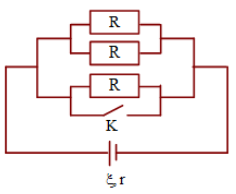
\includegraphics{../figs/VN11-2021-PH-TP016-1.png}
		\end{center}
	Các điện trở có giá trị bằng nhau $R=\SI{6}{\Omega}$. Nguồn điện có suất điện động $\calE=\SI{3}{V}$, điện trở trong $r=\SI{2}{\Omega}$. Điện trở của các dây nối và khóa K không đáng kể. Cường độ dòng điện chạy qua nguồn khi đóng khóa K có giá trị bằng
		\begin{mcq}(4)
			\item $\SI{1.5}{A}$.
			\item $\SI{0.75}{A}$.
			\item $\SI{0.15}{A}$.
			\item $\SI{0.6}{A}$.
		\end{mcq}
		
	}
	\loigiai
	{	\textbf{Đáp án: A.}
		
		Khi đóng khóa K thì mạch bị nối tắt, nên điện trở mạch ngoài bằng không.
		
		Cường độ dòng điện qua mạch:
		$$I=\dfrac{\calE}{r} = \SI{1.5}{A}.$$
	}
	\item \mkstar{2}
	
	\cauhoi
	{Cho mạch điện như hình vẽ.
		\begin{center}
			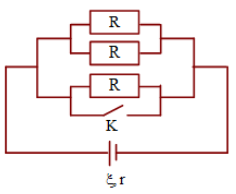
\includegraphics{../figs/VN11-2021-PH-TP016-1.png}
		\end{center}
		Các điện trở có giá trị bằng nhau $R=\SI{6}{\Omega}$. Nguồn điện có suất điện động $\calE=\SI{3}{V}$, điện trở trong $r=\SI{2}{\Omega}$. Điện trở của các dây nối và khóa K không đáng kể. Cường độ dòng điện chạy qua nguồn khi mở khóa K có giá trị bằng
	\begin{mcq}(4)
		\item $\SI{1.5}{A}$.
		\item $\SI{0.75}{A}$.
		\item $\SI{0.15}{A}$.
		\item $\SI{0.6}{A}$.
	\end{mcq}
		
	}
	\loigiai
	{	\textbf{Đáp án: B.}
		
		Khi mở khóa K thì khi đó đoạn mạch gồm ($R$ song song $R$) song song $R$, tương đương với 3 điện trở $R$ mắc song song.
		
		Điện trở tương đương:
		$$R_\text{tđ} = \dfrac{R}{3} = \SI{2}{\Omega}.$$
		
		Cường độ dòng điện qua mạch:
		$$I=\dfrac{\calE}{R_\text{tđ} + r} = \SI{0.75}{A}.$$
	}
	\item \mkstar{2}
	
	\cauhoi
	{Cho mạch điện như hình dưới.
		\begin{center}
			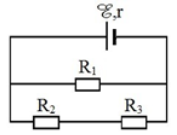
\includegraphics{../figs/VN11-2021-PH-TP016-2.png}
		\end{center}
	Biết $\calE = \SI{12}{V}$, $r=\SI{1}{\Omega}$, $R_1=\SI{5}{\Omega}$, $R_2=R_3=\SI{10}{\Omega}$. Bỏ qua điện trở của dây nối. Hiệu điện thế giữa hai đầu $R_1$ là
		\begin{mcq}(4)
			\item $\SI{10.2}{V}$.
			\item $\SI{4.8}{V}$.
			\item $\SI{9.6}{V}$.
			\item $\SI{7.6}{V}$.
		\end{mcq}
		
	}
	\loigiai
	{	\textbf{Đáp án: C.}
		
		Hiệu điện thế giữa hai đầu $R_1$ cũng là hiệu điện thế mạch ngoài.
		
		Điện trở tương đương mạch ngoài:
		$$R=\dfrac{R_{23} R_1}{R_{23} + R_1} = \SI{4}{\Omega}.$$
		
		Cường độ dòng điện toàn mạch:
		$$I=\dfrac{\calE}{R + r} = \SI{2.4}{A}.$$
		
		Hiệu điện thế mạch ngoài:
		$$U=IR = \SI{9.6}{V}.$$
		
		Vậy $U_1 = U = \SI{9.6}{V}$.
	}
	\item \mkstar{2}
	
	\cauhoi
	{Cho mạch điện như hình dưới.
		\begin{center}
			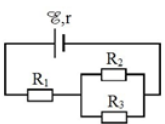
\includegraphics{../figs/VN11-2021-PH-TP016-3.png}
		\end{center}
	Biết $\calE = \SI{9}{V}$, $r=\SI{1}{\Omega}$, $R_1=\SI{5}{\Omega}$, $R_2=\SI{20}{\Omega}$, $R_3=\SI{30}{\Omega}$. Bỏ qua điện trở của dây nối. Hiệu điện thế giữa hai đầu $R_1$ là
		\begin{mcq}(4)
			\item $\SI{8.5}{V}$.
			\item $\SI{6.0}{V}$.
			\item $\SI{4.5}{V}$.
			\item $\SI{2.5}{V}$.
		\end{mcq}
		
	}
	\loigiai
	{	\textbf{Đáp án: D.}
		
		Điện trở tương đương mạch ngoài:
		$$R=R_1 + R_{23} = \SI{17}{\Omega}.$$
		
		Cường độ dòng điện qua mạch:
		$$I=\dfrac{\calE}{R + r} = \SI{0.5}{A}.$$
		
		Hiệu điện thế giữa hai đầu $R_1$:
		$$U_1 = I R_1 = \SI{2.5}{V}.$$
	}
	\item \mkstar{3}
	
	\cauhoi
	{Cho mạch điện như hình vẽ.
		\begin{center}
			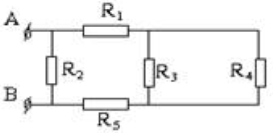
\includegraphics{../figs/VN11-2021-PH-TP016-4.png}
		\end{center}
	
	Trong đó: $R_1=R_3=R_5=\SI{3}{\Omega}$, $R_2=\SI{8}{\Omega}$, $R_4=\SI{6}{\Omega}$, $U_5 = \SI{6}{V}$. Tính điện trở tương đương của đoạn mạch AB và cường độ dòng điện chạy qua từng điện trở.
		\begin{mcq}
			\item $R=\SI{4}{\Omega}$, $I_1=I_5=\SI{2}{A}$, $I_3=\xsi{4/3}{A}$, $I_4=\xsi{2/3}{A}$, $I_2=\SI{2}{A}$.
			\item $R=\SI{8}{\Omega}$, $I_1=I_5=\SI{2}{A}$, $I_3=\xsi{4/3}{A}$, $I_4=\xsi{2/3}{A}$, $I_2=\SI{2}{A}$.
			\item $R=\SI{4}{\Omega}$, $I_1=I_5=\SI{1}{A}$, $I_3=\xsi{4/3}{A}$, $I_4=\xsi{2/3}{A}$, $I_2=\SI{2}{A}$.
			\item $R=\SI{8}{\Omega}$, $I_1=I_5=\SI{2}{A}$, $I_3=\xsi{2/3}{A}$, $I_4=\xsi{4/3}{A}$, $I_2=\SI{2}{A}$.
		\end{mcq}
		
	}
	\loigiai
	{	\textbf{Đáp án: A.}
		
		Điện trở thành phần:
		$$R_{34} = \dfrac{R_3 R_4}{R_3 + R_4} = \SI{2}{\Omega}.$$
		
		$$R_{1345} = R_1 + R_{34} + R_5 = \SI{8}{\Omega}.$$
		
		$$R=\dfrac{R_2 R_{1345}}{R_2 + R_{1345}} = \SI{4}{\Omega}.$$
		
		Cường độ dòng điện:
		$$I_5 = I_{34} = I_1 = I_{1345} = \dfrac{U_5}{R_5} = \SI{2}{A}.$$
		
		Hiệu điện thế:
		$$U_{34} = U_3 = U_4 = I_{34} R_{34} = \SI{4}{V}.$$
		
		Suy ra:
		$$I_3 = \dfrac{U_3}{R_3} = \xsi{\dfrac{4}{3}}{A};\ I_4 = \dfrac{U_4}{R_4} = \xsi{\dfrac{2}{3}}{A};\ U_{1345} = U_2 = U_\text{AB} = I_{1345} R_{1345} = \SI{16}{V};\ I_2 = \dfrac{U_2}{R_2} = \SI{2}{A}.$$
	}
	\item \mkstar{3}
	
	\cauhoi
	{Cho mạch điện như hình vẽ.
		\begin{center}
			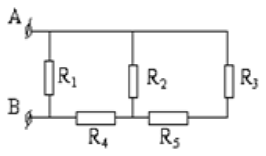
\includegraphics{../figs/VN11-2021-PH-TP016-5.png}
		\end{center}
	Trong đó: $R_1 = \SI{8}{\Omega}$, $R_3=\SI{10}{\Omega}$, $R_2=R_4=R_5=\SI{20}{\Omega}$, $I_3=\SI{2}{A}$. Tính điện trở tương đương của đoạn mạch AB và cường độ dòng điện chạy qua từng điện trở.
		\begin{mcq}
			\item $R=\SI{6.4}{\Omega}$, $I_1=\SI{20}{A}$, $I_2=\SI{3}{A}$, $I_3=I_5=\SI{2}{A}$, $I_4=\SI{5}{A}$.
			\item $R=\SI{32}{\Omega}$, $I_1=\SI{20}{A}$, $I_2=\SI{3}{A}$, $I_3=I_5=\SI{2}{A}$, $I_4=\SI{5}{A}$.
			\item $R=\SI{32}{\Omega}$, $I_1=\SI{4}{A}$, $I_2=\SI{3}{A}$, $I_3=I_5=\SI{2}{A}$, $I_4=\SI{5}{A}$.
			\item $R=\SI{6.4}{\Omega}$, $I_1=\SI{4}{A}$, $I_2=\SI{3}{A}$, $I_3=I_5=\SI{2}{A}$, $I_4=\SI{5}{A}$.
		\end{mcq}
		
	}
	\loigiai
	{	\textbf{Đáp án: A.}
		
		Điện trở thành phần:
		$$R_{35} = R_3 + R_5 = \SI{30}{\Omega}.$$
		
		$$R_{235} = \dfrac{R_2 R_{35}}{R_2 + R_{35}} = \SI{12}{\Omega}.$$
		
		$$R_{4235} = R_4 + R_{235} = \SI{32}{\Omega}.$$
		
		$$R=\dfrac{R_1 R_{4235}}{R_1 + R_{4235}} = \SI{6.4}{\Omega}.$$
		
		Cường độ dòng điện:
		$$I_3 = I_5 = I_{35} = \SI{2}{A}.$$
		
		Hiệu điện thế:
		$$U_{35} = U_2 = U_{235} = I_{35} R_{35} = \SI{60}{V}.$$
		
		Suy ra:
		$$I_2 = \dfrac{U_2}{R_2} = \SI{3}{A};\ I_{235} = I_4 = I_{4235} = \SI{5}{A};\ U_{4235} = U_1 = U_\text{AB} = I_{4235} R_{4235} = \SI{160}{V};\ I_1 = \dfrac{U_1}{R_1} = \SI{20}{A}.$$
	}
	\item \mkstar{3}
	
	\cauhoi
	{Cho mạch điện như hình vẽ.
		\begin{center}
			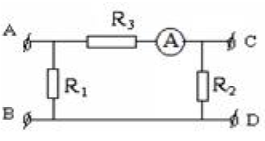
\includegraphics{../figs/VN11-2021-PH-TP016-6.png}
		\end{center}
	Nếu đặt vào AB một hiệu điện thế 100 V thì người ta lấy ra ở hai đầu CD một hiệu điện thế 40 V và ampe kế chỉ 1 A. Nếu đặt vào CD một hiệu điện thế 60 V thì người ta lấy ra ở AB một hiệu điện thế 15 V. Coi điện trở của ampe kế không đáng kể. Tính giá trị của mỗi điện trở.
		\begin{mcq}(2)
			\item $R_1=\SI{30}{\Omega}$, $R_2=\SI{40}{\Omega}$, $R_3=\SI{50}{\Omega}$.
			\item $R_1=\SI{20}{\Omega}$, $R_2=\SI{40}{\Omega}$, $R_3=\SI{60}{\Omega}$.
			\item $R_1=\SI{20}{\Omega}$, $R_2=\SI{30}{\Omega}$, $R_3=\SI{40}{\Omega}$.
			\item $R_1=\SI{30}{\Omega}$, $R_2=\SI{40}{\Omega}$, $R_3=\SI{60}{\Omega}$.
		\end{mcq}
		
	}
	\loigiai
	{	\textbf{Đáp án: B.}
		
		Trường hợp đặt vào giữa A và B hiệu điện thế $\SI{100}{V}$ thì đoạn mạch có: ($R_3$ nối tiếp $R_2$) song song $R_1$, nên:
		$$I_3 = I_2 = I_\text{A} = \SI{1}{A}.$$
		
		$$R_2 = \dfrac{U_\text{CD}}{I_2} = \SI{40}{\Omega}.$$
		
		$$U_\text{AC} = U_\text{AB} - U_\text{CD} = \SI{60}{V}.$$
		
		$$R_3 = \dfrac{U_\text{AC}}{I_3} = \SI{60}{\Omega}.$$
		
		Trường hợp đặt vào giữa C và D hiệu điện thế $\SI{60}{V}$ thì đoạn mạch có: ($R_3$ nối tiếp $R_1$) song song $R_2$. Khi đó:
		$$U_\text{AC} = U_\text{CD} - U_\text{AB} = \SI{45}{V}.$$
		
		$$I_3 = I_1 = \dfrac{U_\text{AC}}{R_3} = \SI{0.75}{A}.$$
		
		$$R_1 = \dfrac{U_\text{AB}}{I_1} = \SI{20}{\Omega}.$$
	}
	\item \mkstar{3}
	
	\cauhoi
	{Cho mạch điện như hình vẽ.
		\begin{center}
			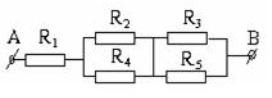
\includegraphics{../figs/VN11-2021-PH-TP016-7.png}
		\end{center}
	Trong đó: $R_1=\SI{2.4}{\Omega}$, $R_3=\SI{4}{\Omega}$, $R_2=\SI{14}{\Omega}$, $R_4=R_5=\SI{6}{\Omega}$, $I_3=\SI{2}{A}$. Tính điện trở tương đương của đoạn mạch AB và hiệu điện thế giữa hai đầu các điện trở.
			\begin{mcq}
			\item $R=\SI{12}{\Omega}$, $U_2 = U_4 = \SI{8}{V}$, $U_1=\SI{8}{V}$, $U_3=U_5=\SI{14}{V}$.
			\item $R=\SI{12}{\Omega}$, $U_2 = U_4 = \SI{14}{V}$, $U_1=\SI{6}{V}$, $U_3=U_5=\SI{8}{V}$.
			\item $R=\SI{12}{\Omega}$, $U_2 = U_4 = \SI{14}{V}$, $U_1=\SI{4}{V}$, $U_3=U_5=\SI{8}{V}$.
			\item $R=\SI{9}{\Omega}$, $U_2 = U_4 = \SI{14}{V}$, $U_1=\SI{8}{V}$, $U_3=U_5=\SI{8}{V}$.
		\end{mcq}
		
	}
	\loigiai
	{	\textbf{Đáp án: D.}
		
		Đoạn mạch gồm: $R_1$ nối tiếp ($R_2$ song song $R_4$) nối tiếp ($R_3$ song song $R_5$).
		
		Điện trở thành phần:
		$$R_{24} = \dfrac{R_2 R_4}{R_2 + R_4} = \SI{4.2}{\Omega}.$$
		
		$$R_{35} = \dfrac{R_3 R_5}{R_3 + R_5} = \SI{2.4}{\Omega}.$$
		
		$$R=R_1 + R_{24} + R_{35} = \SI{9}{\Omega}.$$
		
		Hiệu điện thế:
		$$U_3 = U_5 = U_{35} = I_3 R_3 = \SI{8}{V}.$$
		
		Suy ra:
		$$I_{35} = I_{24} = I_1 = I = \dfrac{U_{35}}{R_{35}} = \xsi{\dfrac{10}{3}}{A};\ U_{24} = U_2 = U_4 = I_{24} R_{24} = \SI{14}{V};\ U_1 = I_1 R_1 = \SI{8}{V}.$$
	}
	\item \mkstar{4}
	
	\cauhoi
	{Cho mạch điện như hình vẽ.
		\begin{center}
			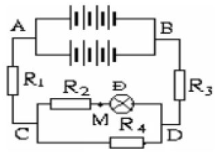
\includegraphics{../figs/VN11-2021-PH-TP016-8.png}
		\end{center}
	Trong đó: bộ nguồn gồm 8 ắcquy, mỗi ắcquy có suất điện động $\calE=\SI{2}{V}$, điện trở trong $r=\SI{0.4}{\Omega}$ mắc thành hai nhánh, mỗi nhánh có 4 nguồn mắc nối tiếp; đèn loại 6 V - 6 W; $R_1=\SI{0.2}{\Omega}$, $R_2=\SI{6}{\Omega}$, $R_3=\SI{4}{\Omega}$ và $R_4=\SI{4}{\Omega}$. Chọn phương án đúng.
		\begin{mcq}(2)
			\item $U_\text{AM} = \SI{-3.4}{V}$ và đèn sáng mạnh.
			\item $U_\text{AM} = \SI{3.4}{V}$ và đèn sáng yếu.
			\item $U_\text{AM} = \SI{-1.7}{V}$ và đèn sáng mạnh.
			\item $U_\text{AM} = \SI{1.7}{V}$ và đèn sáng yếu.
		\end{mcq}
		
	}
	\loigiai
	{	\textbf{Đáp án: D.}
		
		Ta có:
		$$\calP_\text{đ} = I_\text{đ}^2 R_\text{đ} = \dfrac{U_\text{đ}^2}{R_\text{đ}} \Rightarrow R_\text{đ} = \dfrac{U_\text{đ}^2}{\calP_\text{đ}} = \SI{6}{\Omega}.$$
		
		Mạch gồm: $R_1$ nối tiếp [$R_4$ song song ($R_2$ nối tiếp $R_\text{đ}$)] nối tiếp $R_3$.
		$$R_\text{2đ} = R_2 + R_\text{đ} = \SI{12}{\Omega}$$
		
		$$R_\text{2đ4} = \dfrac{R_\text{2đ} R_4}{R_{\text{2đ} + R_4}} = \SI{3}{\Omega}.$$
		
		$$R=R_1 + R_\text{2đ4} + R_3 = \SI{7.2}{\Omega}.$$
		
		Mà:
		$$\calE_\text{b} = 4 \calE = \SI{8}{V};\ r_\text{b} = \dfrac{4r}{2} = \SI{0.8}{\Omega}.$$
		
		$$\Rightarrow I = \dfrac{\calE_\text{b}}{R+r_\text{b}} = \SI{1}{A}.$$
		
		Ta tính được:
		$$U_\text{AC} = I R_1 = \SI{0.2}{V}.$$
		
		$$U_\text{CM} = I_\text{2đ} R_2 = \dfrac{U_\text{2đ}}{R_\text{2đ}} R_2 = \dfrac{U_\text{2đ4}}{R_\text{2đ}} R_2 = \dfrac{I R_\text{2đ4}}{R_\text{2đ}} R_2 = \SI{1.5}{V}.$$
		
		Suy ra:
		$$U_\text{AM} = U_\text{AC} + U_\text{CM} = \SI{1.7}{V}.$$
	}
\end{enumerate}

\whiteBGstarEnd

\loigiai
{
	\begin{center}
		\textbf{BẢNG ĐÁP ÁN}
	\end{center}
	\begin{center}
		\begin{tabular}{|m{2.8em}|m{2.8em}|m{2.8em}|m{2.8em}|m{2.8em}|m{2.8em}|m{2.8em}|m{2.8em}|m{2.8em}|m{2.8em}|}
			\hline
			1.C  & 2.A  & 3.B  & 4.D  & 5.B  & 6.C  & 7.B  & 8.D  & 9.B  & 10.C  \\
			\hline
			11.D  & 12.A  & 13.B  & 14.C  & 15.D  & 16.A  & 17.A  & 18.B  & 19.D  & 20.D  \\
			\hline
		\end{tabular}
	\end{center}
}
\section{Tự luận}
\begin{enumerate}[label=\bfseries Câu \arabic*:]
	\item \mkstar{1}
	
	\cauhoi{
		Toàn mạch là gì? Phát biểu định luật Ôm cho toàn mạch.
	}
	
	\loigiai{
		
		Toàn mạch là mạch điện gồm nguồn điện có suất điện động $\calE$ và điện trở trong $r$ hoặc gồm các nguồn điện được ghép thành bộ, nối với mạch ngoài gồm các điện trở hoặc các vật dẫn được coi như là điện trở.
		
		Định luật Ôm đối với toàn mạch: Cường độ dòng điện chạy trong mạch kín tỉ lệ thuận với suất điện động của nguồn điện và tỉ lệ nghịch với điện trở toàn phần của mạch đó.
		$$I=\dfrac{\calE}{R_\text{N} + r}.$$
	}
	
	\item \mkstar{2}
	
	\cauhoi{
		Một đoạn mạch gồm điện trở $R_1=\SI{100}{\Omega}$ mắc nối tiếp với điện trở $R_2=\SI{200}{\Omega}$, hiệu điện thế giữa hai đầu đoạn mạch là 12 V. Tính hiệu điện thế giữa hai đầu điện trở $R_1$.
	}
	
	\loigiai{
		
		Điện trở tương đương của mạch ngoài:
		$$R=R_1 + R_2 = \SI{300}{\Omega}.$$
		
		Cường độ dòng điện toàn mạch cũng chính là cường độ dòng điện đi qua $R_1$:
		$$I_1 = I =\dfrac{U}{R} = \SI{0.04}{A}.$$
		
		Hiệu điện thế giữa hai đầu $R_1$:
		$$U_1 = U R_1 = \SI{4}{V}.$$
	}
	\item \mkstar{3}
	
	\cauhoi{
	Cho mạch điện như hình vẽ.
	\begin{center}
		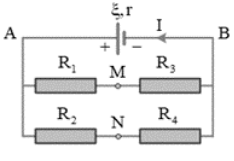
\includegraphics{../figs/VN11-2021-PH-TP016-9.png}
	\end{center}
	Cho $r=\SI{1}{\Omega}$, $R_1=\SI{1}{\Omega}$, $R_2=\SI{4}{\Omega}$, $R_3=\SI{3}{\Omega}$, $R_4=\SI{8}{\Omega}$ và $U_\text{MN} = \SI{1.5}{V}$. Điện trở của các dây nối không đáng kể. Tính suất điện động của nguồn.
	}
	
	\loigiai{
		
		Điện trở tương đương của mạch ngoài:
		$$R=\dfrac{(R_1 + R_3) (R_2 + R_4)}{(R_1 + R_3) + (R_2 + R_4)} = \SI{3}{\Omega}.$$
		
		Hiệu điện thế mạch ngoài:
		$$U_\text{AB} = I R = I_{13} (R_1 + R_3) = I_{24} (R_2 + R_4).$$
		
		Ta được hệ phương trình:
		$$
		\begin{cases}
			I_{13} = I \dfrac{R}{R_1 + R_3} = \SI{0.75}{} I \\
			I_{24} = I \dfrac{R}{R_2 + R_4} = \SI{0.25}{} I.
		\end{cases}
		$$
		
		Xét hiệu điện thế $U_\text{MN}$, ta có:
		$$U_\text{MN} = U_\text{MB} + U_\text{BN} = U_\text{MB} - U_\text{NB} = I_{13} R_3 - I_{24} R_4.$$
		
		Mà $U_\text{MN} = \SI{1.5}{V}$, suy ra:
		$$\SI{1.5}{} = \SI{0.75}{} I \cdot 3 - \SI{0.25}{} I \cdot 8 \Rightarrow I = \SI{6}{A}.$$
		
		Suất điện động của nguồn:
		$$\calE = I (R+r) = \SI{24}{V}.$$
	}
	\item \mkstar{4}
	
	\cauhoi{
		Để xác định điện trở trong của một nguồn điện, một học sinh mắc mạch điện như hình $\text{H}_1$ bên dưới. Đóng khóa K và điều chỉnh con chạy C, kết quả đo được mô tả bởi đồ thị biểu diễn sự phụ thuộc của chỉ số $U$ của vôn kế vào chỉ số $I$ của ampe kế A như hình $\text{H}_2$.
		\begin{center}
			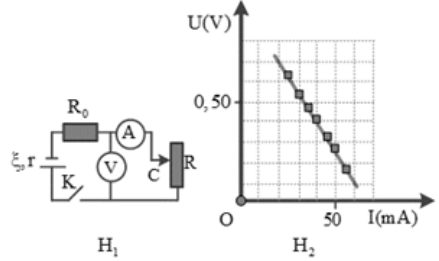
\includegraphics{../figs/VN11-2021-PH-TP016-10.png}
		\end{center}
	Điện trở của vôn kế rất lớn. Biết $R_0=\SI{14}{\Omega}$. Giá trị trung bình của $r$ được xác định bởi thí nghiệm này là bao nhiêu?
	}
	
	\loigiai{
		
		Từ biểu thức:
		$$\dfrac{\calE}{I} = R + R_0 + r.$$
		
		Với $R=\dfrac{U}{I}$, suy ra:
		$$\dfrac{\calE}{I} = \dfrac{U}{I} + R_0 + r.$$
		
		Phương trình trên tương đương với hệ:
		$$
		\begin{cases}
			\dfrac{\calE}{\SI{20e-3}{}} = \dfrac{\SI{0.7}{}}{\SI{20e-3}{}} + 14 + r \\
			\dfrac{\calE}{\SI{60e-3}{}} = \dfrac{\SI{0.1}{}}{\SI{60e-3}{}} + 14 + r
		\end{cases}
		$$
		
		Ta tính được $r=\SI{1}{\Omega}$ và $\calE = \SI{1}{V}$.
		
		Vậy giá trị trung bình của $r$ là $\SI{1}{\Omega}$.
	}
	\item \mkstar{4}
	
	\cauhoi{
		Cho mạch điện như hình vẽ.
		\begin{center}
			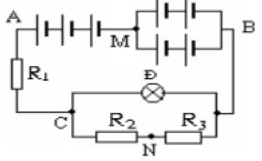
\includegraphics{../figs/VN11-2021-PH-TP016-11.png}
		\end{center}
	Trong đó có 7 nguồn giống nhau, mỗi nguồn có suất điện động $\calE = \SI{2}{V}$, điện trở trong $r=\SI{0.2}{\Omega}$ mắc như hình vẽ. Đèn thuộc loại 6 V - 12 W, cho $R_1=\SI{2.2}{\Omega}$, $R_2=\SI{4}{\Omega}$, $R_3=\SI{2}{\Omega}$. Tính hiệu điện thế $U_\text{MN}$.
	}
	
	\loigiai{
		
		Khi $R_1$ nối tiếp $R_2$ thì cường độ dòng điện qua mỗi điện trở là
		$$I = \dfrac{\calE}{R_1 + R_2 + r} \Rightarrow R_1 + R_2 = \SI{0.9}{\Omega}\ (*).$$
		
		Khi $R_1$ song song $R_2$ thì cường độ dòng điện tổng cộng qua hai điện trở là
		$$I=\dfrac{\calE}{\dfrac{R_1 R_2}{R_1 + R_2} + r} \Rightarrow \dfrac{R_1 R_2}{R_1 + R_2} = \SI{0.2}{\Omega}\ (**).$$
		
		Từ $(*)$ và $(**)$, tính được:
		$$R_1 = \SI{0.6}{\Omega};\ R_2 = \SI{0.3}{\Omega}.$$
	}
	
\end{enumerate}
\stopcontents[mychapters]
\chapter{Ôn tập: Chương II. Dòng điện không đổi}
\whiteBGstarBegin
\setcounter{section}{0}
\section{Trắc nghiệm}
\begin{enumerate}[label=\bfseries Câu \arabic*:]
	
	
	\item \mkstar{1}
	
	\cauhoi
	{Điện năng được đo bằng
		\begin{mcq}(2)
			\item vôn kế.
			\item công tơ điện.
			\item ampe kế.
			\item tĩnh điện kế.
		\end{mcq}
		
	}
	\loigiai
	{	\textbf{Đáp án: B.}
		
		Điện năng được đo bằng công tơ điện.
	}
	\item \mkstar{1}
	
	\cauhoi
	{Công suất điện được đo bằng đơn vị nào sau đây?
		\begin{mcq}(2)
			\item Niu-tơn (N).
			\item Jun (J).
			\item Oát (W).
			\item Culông (C).
		\end{mcq}
		
	}
	\loigiai
	{	\textbf{Đáp án: C.}
		
		Công suất điện được đo bằng đơn vị Oát (W).
	}
	\item \mkstar{1}
	
	\cauhoi
	{Công suất của nguồn điện được xác định bằng
		\begin{mcq}
			\item lượng điện tích mà nguồn điện sản ra trong 1 giây.
			\item công mà lực lạ thực hiện khi dịch chuyển 1 đơn vị điện tích dương ngược chiều điện trường bên trong nguồn điện.
			\item lượng điện tích chạy qua nguồn điện trong 1 giây.
			\item công của lực điện thực hiện khi dịch chuyển 1 đơn vị điện tích dương chạy trong mạch điện kín trong 1 giây.
		\end{mcq}
		
	}
	\loigiai
	{	\textbf{Đáp án: D.}
		
		Công suất của nguồn điện được xác định bằng công của lực điện thực hiện khi dịch chuyển 1 đơn vị điện tích dương chạy trong mạch điện kín trong 1 giây.
	}
	\item \mkstar{1}
	
	\cauhoi
	{Khi một động cơ điện đang hoạt động thì điện năng được biến đổi thành
		\begin{mcq}
			\item năng lượng cơ học.
			\item năng lượng cơ học và năng lượng nhiệt.
			\item năng lượng cơ học, năng lượng nhiệt và năng lượng điện trường.
			\item năng lượng cơ học, năng lượng nhiệt và năng lượng ánh sáng.
		\end{mcq}
		
	}
	\loigiai
	{	\textbf{Đáp án: B.}
		
		Khi một động cơ điện đang hoạt động thì điện năng được biến đổi thành năng lượng cơ học và năng lượng nhiệt.
	}
	\item \mkstar{2}
	
	\cauhoi
	{Cho mạch điện gồm một pin $\SI{1.5}{V}$ có điện trở trong $\SI{0.5}{\Omega}$ nối với mạch ngoài là một điện trở $\SI{2.5}{\Omega}$. Cường độ dòng điện trong toàn mạch là
		\begin{mcq}(4)
			\item $\SI{3}{A}$.
			\item $\SI{0.6}{A}$.
			\item $\SI{0.5}{A}$.
			\item $\SI{2}{A}$.
		\end{mcq}
		
	}
	\loigiai
	{	\textbf{Đáp án: C.}
		
		Áp dụng định luật Ôm toàn mạch:
		$$I=\dfrac{\calE}{R + r} = \SI{0.5}{A}.$$
	}
	\item \mkstar{2}
	
	\cauhoi
	{Một mạch điện gồm có nguồn là một pin $\SI{9}{V}$, điện trở mạch ngoài $\SI{4}{\Omega}$, cường độ dòng điện trên toàn mạch là $\SI{2}{A}$. Điện trở trong của nguồn là
		\begin{mcq}(4)
			\item $\SI{0.5}{\Omega}$.
			\item $\SI{4.5}{\Omega}$.
			\item $\SI{1}{\Omega}$.
			\item $\SI{2}{\Omega}$.
		\end{mcq}
		
	}
	\loigiai
	{	\textbf{Đáp án: A.}
		
		Áp dụng định luật Ôm toàn mạch:
		$$I=\dfrac{\calE}{R + r} \Rightarrow r = \SI{0.5}{\Omega}.$$
	}
	\item \mkstar{2}
	
	\cauhoi
	{Cho mạch điện gồm hai pin có suất điện động và điện trở trong của mỗi pin là $\SI{1.5}{V} - \SI{0.5}{\Omega}$ mắc nối tiếp rồi nối với mạch ngoài là một điện trở $\SI{2}{\Omega}$. Cường độ dòng điện toàn mạch là
		\begin{mcq}(4)
			\item $\SI{3}{A}$.
			\item $\SI{0.6}{A}$.
			\item $\SI{1}{A}$.
			\item $\SI{2}{A}$.
		\end{mcq}
		
	}
	\loigiai
	{	\textbf{Đáp án: C.}
		
		Suất điện động của bộ nguồn:
		$$\calE_\text b = 2\calE = \SI{3}{V}.$$
		
		Điện trở trong của bộ nguồn:
		$$r_\text b = 2 r = \SI{1}{\Omega}.$$
		
		Cường độ dòng điện toàn mạch:
		$$I=\dfrac{\calE_\text b}{R + r_\text b} = \SI{1}{A}.$$
	}
	\item \mkstar{2}
	
	\cauhoi
	{Một mạch điện gồm có nguồn là một pin $\SI{9}{V}$, điện trở trong $\SI{0.5}{\Omega}$ và mạch ngoài gồm hai điện trở $\SI{8}{\Omega}$ mắc song song. Cường độ dòng điện trên toàn mạch là
		\begin{mcq}(4)
			\item $\SI{2}{A}$.
			\item $\SI{4.5}{A}$.
			\item $\SI{1}{A}$.
			\item $\xsi{\dfrac{18}{33}}{A}$.
		\end{mcq}
		
	}
	\loigiai
	{	\textbf{Đáp án: A.}
		
		Điện trở tương đương mạch ngoài:
		$$R = \dfrac{\SI{8}{\Omega}}{2} = \SI{4}{\Omega}.$$
		
		Cường độ dòng điện toàn mạch:
		$$I=\dfrac{\calE}{R + r} = \SI{2}{A}.$$
	}
	\item \mkstar{2}
	
	\cauhoi
	{Hai bóng đèn sợi đốt cùng công suất định mức, có các hiệu điện thế định mức lần lượt là $U_1$ và $U_2$. Xác định tỉ số điện trở $\dfrac{R_1}{R_2}$ của hai bóng đèn theo $U_1$ và $U_2$.
		\begin{mcq}(4)
			\item $\dfrac{R_1}{R_2} = \left(\dfrac{U_1}{U_2}\right)^2$.
			\item $\dfrac{R_1}{R_2} = \dfrac{U_2}{U_1}$.
			\item $\dfrac{R_1}{R_2} = \dfrac{U_1}{U_2}$.
			\item $\dfrac{R_1}{R_2} = \left(\dfrac{U_2}{U_1}\right)^2$.
		\end{mcq}
		
	}
	\loigiai
	{	\textbf{Đáp án: A.}
		
		Từ biểu thức tính điện trở theo công suất định mức: $R=\dfrac{U_\text{đm}^2}{\calP}$, suy ra:
		$$\dfrac{R_1}{R_2} = \left(\dfrac{U_1}{U_2}\right)^2.$$
	}
	\item \mkstar{2}
	
	\cauhoi
	{Tính hiệu suất của một bếp điện nếu sau $t=20$ phút nó đun sôi được $\SI{2}{l}$ nước từ nhiệt độ ban đầu $\SI{20}{\celsius}$. Biết rằng cường độ dòng điện chạy qua bếp là $I=\SI{3}{A}$, hiệu điện thế đặt vào là $U=\SI{220}{V}$.
		\begin{mcq}(4)
			\item $H=\SI{75}{\percent}$.
			\item $H=\SI{85}{\percent}$.
			\item $H=\SI{95}{\percent}$.
			\item $H=\SI{65}{\percent}$.
		\end{mcq}
		
	}
	\loigiai
	{	\textbf{Đáp án: B.}
		
		Nhiệt lượng (công có ích):
		$$Q=mc \Delta t = \SI{672000}{J}.$$
		
		Điện năng tiêu thụ (công toàn phần):
		$$A=UI t = \SI{792000}{J}.$$
		
		Hiệu suất của bếp điện:
		$$H=\dfrac{Q}{A} = \SI{85}{\percent}.$$
	}
	\item \mkstar{2}
	
	\cauhoi
	{Cho mạch điện như hình vẽ.
		\begin{center}
			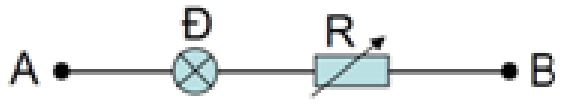
\includegraphics[scale=0.6]{../figs/VN11-2021-PH-TP017-1}
		\end{center}
	
	Hiệu điện thế giữa hai đầu đoạn mạch là $\SI{15}{V}$, trên đèn có ghi $\SI{12}{V} - \SI{6}{W}$, điện trở dây nối không đáng kể. Hãy xác định giá trị của biến trở để đèn sáng bình thường.
		\begin{mcq}(4)
			\item $R=\SI{1}{\Omega}$.
			\item $R=\SI{3}{\Omega}$.
			\item $R=\SI{6}{\Omega}$.
			\item $R=\SI{9}{\Omega}$.
		\end{mcq}
		
	}
	\loigiai
	{	\textbf{Đáp án: C.}
		
		Điện trở của đèn:
		$$R_\text{đ} = \dfrac{U_\text{đm}^2}{\calP} = \SI{24}{\Omega}.$$
		
		Để đèn sáng bình thường thì cường độ dòng điện qua mạch là
		$$I=\dfrac{\calP_\text{đm}}{U_\text{đm}} = \SI{0.5}{A}.$$
		
		Vậy giá trị biến trở cần tìm là
		$$I=\dfrac{U}{R + R_\text{đ}} \Rightarrow R = \SI{6}{\Omega}.$$
	}
	\item \mkstar{3}
	
	\cauhoi
	{Một bóng đèn $\SI{100}{V} - \SI{50}{W}$ được mắc vào mạng điện $\SI{240}{V}$. Để đèn sáng bình thường thì cần phải mắc nối tiếp với điện trở $R$ có giá trị
		\begin{mcq}(4)
			\item $R=\SI{280}{\Omega}$.
			\item $R=\SI{880}{\Omega}$.
			\item $R=\SI{200}{\Omega}$.
			\item $R=\SI{120}{\Omega}$.
		\end{mcq}
		
	}
	\loigiai
	{	\textbf{Đáp án: A.}
		
		Điện trở của đèn:
		$$R_\text{đ} = \dfrac{U_\text{đm}^2}{\calP} = \SI{200}{\Omega}.$$
		
		Để đèn sáng bình thường thì cường độ dòng điện qua mạch là
		$$I=\dfrac{\calP_\text{đm}}{U_\text{đm}} = \SI{0.5}{A}.$$
		
		Vậy giá trị điện trở cần tìm là
		$$I=\dfrac{U}{R + R_\text{đ}} \Rightarrow R = \SI{280}{\Omega}.$$
	}
	\item \mkstar{3}
	
	\cauhoi
	{Một nguồn điện có suất điện động $\calE$, điện trở trong $r$ mắc với mạch ngoài là điện trở $R$. Hiệu suất của nguồn điện là $H=\SI{80}{\percent}$. Tỉ số giữa điện trở trong của nguồn ($r$) và điện trở mạch ngoài ($R$) là
		\begin{mcq}(4)
			\item $\SI{0.80}{}$.
			\item $\SI{0.20}{}$.
			\item $\SI{0.40}{}$.
			\item $\SI{0.25}{}$.
		\end{mcq}
		
	}
	\loigiai
	{	\textbf{Đáp án: D.}
		
		Áp dụng công thức tính hiệu suất của nguồn:
		$$H=\dfrac{U}{\calE} = \dfrac{IR}{I(R+r)} = \dfrac{R}{R + r} = \SI{80}{\percent} \Rightarrow \dfrac{r}{R} = \dfrac{1}{4} = \SI{0.25}{}.$$
	}
	\item \mkstar{3}
	
	\cauhoi
	{Một động cơ điện một chiều có điện trở thuần của các cuộn dây là $r=\SI{4}{\Omega}$, mắc nối tiếp với một điện trở $R=\SI{8}{\Omega}$. Tất cả được mắc vào nguồn điện có hiệu điện thế không đổi và bằng $\SI{24}{V}$. Động cơ khi đó hoạt động bình thường và cường độ dòng điện qua động cơ là $\SI{0.5}{A}$. Công suất điện năng chuyển hóa thành cơ năng ở động cơ là
		\begin{mcq}(4)
			\item $\SI{3}{W}$.
			\item $\SI{12}{W}$.
			\item $\SI{10}{W}$.
			\item $\SI{9}{W}$.
		\end{mcq}
		
	}
	\loigiai
	{	\textbf{Đáp án: D.}
		
		Gọi $\calP_\text{đc}$ là công suất điện năng chuyển hóa thành cơ năng của động cơ.
		
		Áp dụng định luật Ôm:
		$$I=\dfrac{U}{R_\text{đc} + R + r} = \SI{0.5}{A} \Rightarrow R_\text{đc} = \SI{36}{\Omega}.$$
		
		Vậy công suất điện năng chuyển hóa thành cơ năng của động cơ là
		$$\calP_\text{đc} = I^2 R_\text{đc} = \SI{9}{W}.$$
	}
	\item \mkstar{3}
	
	\cauhoi
	{Để nạp điện cho một ắc quy có suất điện động $\calE_2 = \SI{6}{V}$, điện trở trong $r_2 = \SI{0.4}{\Omega}$, người ta dùng nguồn điện một chiều có suất điện động $\calE_1 = \SI{12}{V}$, điện trở trong $r_1=\SI{0.2}{\Omega}$ và một biến trở $R$ mắc nối tiếp với ắc quy. Điều chỉnh biến trở đến giá trị $R=\SI{11.4}{\Omega}$, tính công suất điện tiêu thụ ở ắc quy.
		\begin{mcq}(4)
			\item $\SI{9.9}{W}$.
			\item $\SI{9.0}{W}$.
			\item $\SI{3.0}{W}$.
			\item $\SI{3.1}{W}$.
		\end{mcq}
		
	}
	\loigiai
	{	\textbf{Đáp án: D.}
		
		Áp dụng định luật Ôm (với ắc quy đóng vai trò là máy thu):
		$$I=\dfrac{\calE_1 - \calE_2}{R + r_1 + r_2} = \SI{0.5}{A}.$$
		
		Công suất tiêu thụ ở ắc quy bằng tổng công suất nguồn của ắc quy và công suất tỏa nhiệt trên ắc quy:
		$$\calP_2 = \calE_2 I + I^2 r_2 = \SI{3.1}{W}.$$
	}
	\item \mkstar{3}
	
	\cauhoi
	{Cho mạch điện như hình vẽ.
		\begin{center}
			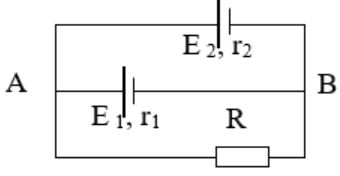
\includegraphics[scale=0.6]{../figs/VN11-2021-PH-TP017-2}
		\end{center}
	
	Trong đó: $\calE_1 = \SI{20}{V}$, $\calE_2 = \SI{32}{V}$, $r_1=\SI{1}{\Omega}$, $r_2=\SI{0.5}{\Omega}$, $R=\SI{2}{\Omega}$. Tìm cường độ dòng điện qua $R$.
		\begin{mcq}(4)
			\item $\SI{4}{A}$.
			\item $\SI{8}{A}$.
			\item $\SI{16}{A}$.
			\item $\SI{12}{A}$.
		\end{mcq}
		
	}
	\loigiai
	{	\textbf{Đáp án: D.}
		
		Hiệu điện thế trên mỗi nhánh:
		$$
		\begin{cases}
			U_\text{AB} = \calE_1 - I_1 r_1 \\
			U_\text{AB} = \calE_2 - I_2 r_2 \\
			U_\text{AB} = IR
		\end{cases}
		$$
		
		Tìm được hệ phương trình:
		$$
		\begin{cases}
			I_1 - \SI{0.5}{} I_2 = \SI{-12}{} \\
			\SI{0.5}{} I_2 + 2I = 32
		\end{cases}
		$$
		
		Mà $I=I_1 +I_2$. Thay vào hệ trên, tìm được $I_1 = \SI{-4}{A}$, $I_2 = \SI{16}{A}$ và $I=\SI{12}{A}$.
	}
	\item \mkstar{3}
	
	\cauhoi
	{Cho mạch điện như hình vẽ.
		\begin{center}
			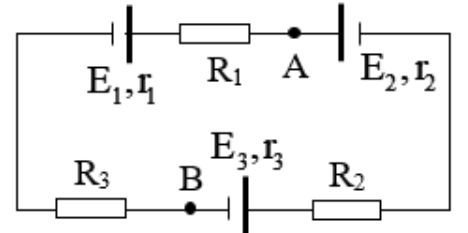
\includegraphics[scale=0.6]{../figs/VN11-2021-PH-TP017-3}
		\end{center}
	
	Cho biết $\calE_1 = \SI{12}{V}$, $r_1=\SI{1}{\Omega}$, $\calE_2 = \SI{6}{V}$, $r_2=\SI{2}{\Omega}$, $\calE_3 = \SI{9}{V}$, $r_3=\SI{3}{\Omega}$, $R_1=\SI{4}{\Omega}$, $R_2=\SI{2}{\Omega}$, $R_3=\SI{3}{\Omega}$. Tính $U_\text{AB}$.
		\begin{mcq}(4)
			\item $U_\text{AB} = \SI{13.6}{V}$.
			\item $U_\text{AB} = \SI{11.6}{V}$.
			\item $U_\text{AB} = \SI{13.2}{V}$.
			\item $U_\text{AB} = \SI{11.2}{V}$.
		\end{mcq}
		
	}
	\loigiai
	{	\textbf{Đáp án: A.}
		
		Áp dụng định luật Ôm cho mạch kín, ta có:
		$$I=\dfrac{\calE_2 + \calE_3 - \calE_1}{R_1 + R_2 + R_3 + r_1 + r_2 + r_3} = \SI{0.2}{A}.$$
		
		Hiệu điện thế $U_\text{AB}$:
		$$U_\text{AB} = \calE_1 + I(R_1 + R_3 + r_1) = \SI{13.6}{V}.$$
	}
	\item \mkstar{3}
	
	\cauhoi
	{Một nguồn điện có suất điện động $\calE = \SI{12}{V}$, điện trở trong $r=\SI{3}{\Omega}$, được mắc với một biến trở $R$ thành mạch kín. Điều chỉnh $R$ để công suất tiêu thụ ở mạch ngoài đạt cực đại. Công suất cực đại đó bằng
		\begin{mcq}(4)
			\item $\SI{144}{W}$.
			\item $\SI{14.4}{W}$.
			\item $\SI{12.0}{W}$.
			\item $\SI{24.0}{W}$.
		\end{mcq}
		
	}
	\loigiai
	{	\textbf{Đáp án: C.}
		
		Áp dụng kết hợp định luật Ôm toàn mạch và biểu thức tính công suất, ta được:
		$$\calP = I^2 R = \dfrac{\calE ^2}{(r+R)^2} R = \dfrac{144 R}{(R+3)^2}.$$
		
		Áp dụng bất đẳng thức Cô-si:
		$$R+3 \geq 2 \sqrt{3 R}.$$
		
		Tính được giá trị cực đại của công suất là
		$$\calP = \dfrac{144 R}{4 \cdot 3R} = \SI{12.0}{W}.$$
	}
	\item \mkstar{3}
	
	\cauhoi
	{Đường đặc trưng Vôn - Ampe của hai vật dẫn có điện trở $R_1$, $R_2$ được cho như hình vẽ.
		\begin{center}
		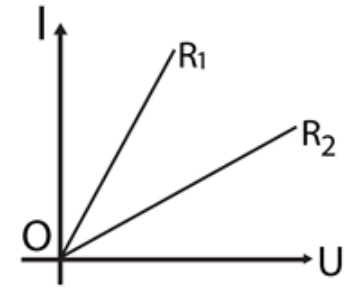
\includegraphics[scale=0.7]{../figs/VN11-2021-PH-TP017-4}
		\end{center}
	
		Chọn kết luận đúng.
		\begin{mcq}(2)
			\item $R_1 < R_2$.
			\item $R_1 > R_2$.
			\item Không thể so sánh $R_1$ với $R_2$.
			\item $R_1=R_2$.
		\end{mcq}
		
	}
	\loigiai
	{	\textbf{Đáp án: A.}
		
		Dựa vào công thức $R=\dfrac{U}{I}$, nhận thấy giá trị này là nghịch đảo của hệ số góc $\tan \alpha$, hay $\dfrac{1}{\tan \alpha} = \dfrac{U}{I}$.
		
		Vậy với $\tan \alpha$ lớn hơn thì $R$ nhỏ hơn. Suy ra $R_1 < R_2$ vì $\tan \alpha_1 > \tan \alpha_2$.
	}
	\item \mkstar{4}
	
	\cauhoi
	{Cho một mạch điện kín gồm nguồn điện có suất điện động $\calE = \SI{12}{V}$, điện trở trong $r=\SI{1.5}{\Omega}$, mạch ngoài gồm điện trở $R_1=\SI{0.5}{\Omega}$ mắc nối tiếp với $R$. Để công suất tiêu thụ trên $R$ đạt cực đại thì giá trị của $R$ là
		\begin{mcq}(4)
			\item $\SI{3}{\Omega}$.
			\item $\SI{2}{\Omega}$.
			\item $\SI{4}{\Omega}$.
			\item $\SI{1}{\Omega}$.
		\end{mcq}
		
	}
	\loigiai
	{	\textbf{Đáp án: B.}
		
		Áp dụng kết hợp định luật Ôm toàn mạch và biểu thức tính công suất, ta được:
		$$\calP = I^2 R = \dfrac{\calE^2}{(r + R_1 + R)^2}R = \dfrac{\calE ^2}{\left(\dfrac{2}{\sqrt{R}} + \sqrt{R}\right)^2}.$$
		
		Áp dụng bất đẳng thức Cô-si:
		$$\dfrac{2}{\sqrt{R}} + \sqrt{R} \geq 2.$$
		
		Vậy giá trị cực đại của công suất đạt được khi $\dfrac{2}{\sqrt{R}} + \sqrt{R} = 2$. Khi đó:
		$$\calP = \dfrac{\calE^2}{2^2} = \SI{36}{W}.$$
		
		Khi đó $R=\SI{2}{\Omega}$.
	}
\end{enumerate}

\whiteBGstarEnd

\loigiai
{
	\begin{center}
		\textbf{BẢNG ĐÁP ÁN}
	\end{center}
	\begin{center}
		\begin{tabular}{|m{2.8em}|m{2.8em}|m{2.8em}|m{2.8em}|m{2.8em}|m{2.8em}|m{2.8em}|m{2.8em}|m{2.8em}|m{2.8em}|}
			\hline
			1.B  & 2.C  & 3.D  & 4.B  & 5.C  & 6.A  & 7.C  & 8.A  & 9.A  & 10.B  \\
			\hline
			11.C  & 12.A  & 13.D  & 14.D  & 15.D  & 16.D  & 17.A  & 18.C  & 19.A  & 20.B  \\
			\hline
		\end{tabular}
	\end{center}
}
\section{Tự luận}
\begin{enumerate}[label=\bfseries Câu \arabic*:]
	\item \mkstar{2}
	
	\cauhoi{
		Một bộ ắc quy có thể cung cấp một dòng điện $\SI{8}{A}$ liên tục trong $\SI{1}{h}$ thì phải nạp lại. Tính suất điện động của ắc quy này nếu trong khoảng thời gian hoạt động trên, nó sản ra một công là $\SI{86.4}{kJ}$.
	}
	
	\loigiai{
		
		Suất điện động của ắc quy này:
		$$\calE = \dfrac{A}{q} = \dfrac{A}{It} = \SI{3}{V}.$$
	}
	
	\item \mkstar{2}
	
	\cauhoi{
		Tính điện năng tiêu thụ và công suất điện khi dòng điện có cường độ $\SI{2}{A}$ chạy qua dây dẫn trong $\SI{1}{h}$. Biết hiệu điện thế giữa hai đầu dây dẫn này là $\SI{6}{V}$.
	}
	
	\loigiai{
		
	Điện năng tiêu thụ:
	$$A= UI t = \SI{43200}{J}.$$
	
	Công suất điện:
	$$\calP = \dfrac{A}{t} = \SI{12}{W}.$$	
	}
	\item \mkstar{2}
	
	\cauhoi{
		Cho ba điện trở giống nhau giá trị $\SI{8}{\Omega}$ gồm hai điện trở mắc song song rồi nối tiếp với điện trở thứ ba. Đoạn mạch này được nối với nguồn điện có điện trở trong $\SI{2}{\Omega}$. Người ta đo được hiệu điện thế giữa hai cực của nguồn là $\SI{12}{V}$. Xác định cường độ dòng điện trong mạch và suất điện động của nguồn điện.
	}
	
	\loigiai{
		
		Điện trở tương đương của mạch ngoài:
		$$R=\dfrac{\SI{8}{\Omega}}{2} + \SI{8}{\Omega} = \SI{12}{\Omega}.$$
		
		Áp dụng công thức xác định hiệu điện thế dựa vào định luật Ôm:
		$$U = \calE - I r \Rightarrow \calE - I r = U \Rightarrow \calE - \dfrac{\calE}{R + r} r = U \Rightarrow \calE= \SI{14}{V}.$$
		
		Cường độ dòng điện trong mạch:
		$$I = \dfrac{\calE}{R + r} = \SI{1}{A}.$$
	}
	\item \mkstar{2}
	
	\cauhoi{
		Một bộ nguồn gồm hai nguồn điện mắc xung đối, nguồn thứ nhất có suất điện động $\calE_1 = \SI{12}{V}$, điện trở trong $r_1=\SI{1}{\Omega}$, nguồn thứ hai có suất điện động $\calE_2 = \SI{4}{V}$, điện trở trong $r_2 = \SI{1}{\Omega}$. Bộ nguồn được mắc với ampe kế có điện trở không đáng kể tạo thành mạch điện kín. Tính hiệu điện thế từ cực dương đến cực âm của nguồn điện $\calE_1$.
	}
	
	\loigiai{
		
		Vì hai nguồn được mắc xung đối nên một trong hai nguồn đóng vai trò là máy thu. Suất điện động của bộ nguồn là
		$$\calE_\text{b} = \SI{12}{V} - \SI{4}{V} = \SI{8}{V}.$$
		
		Điện trở trong của bộ nguồn:
		$$r_\text{b} = r_1 + r_2 = \SI{1}{\Omega} + \SI{1}{\Omega} = \SI{2}{\Omega}.$$
		
		Áp dụng định luật Ôm:
		$$I=\dfrac{\calE_\text b}{R + r_\text b} = \SI{4}{A}.$$
		
		Hiệu điện thế giữa hai cực của $\calE_1$:
		$$U=\calE_1 - I r_1 = \SI{8}{V}.$$
	}
	
\end{enumerate}
\setcounter{mychapter}{12}
\mychapter{Dòng điện trong kim loại}
\startcontents[mychapters]
\printcontents[mychapters]{}{0}{\setcounter{tocdepth}{1}}
\whiteBGstarBegin
\setcounter{section}{0}

\begin{enumerate}[label=\bfseries Câu \arabic*:]
	
	\item \mkstar{1} [34]
	
	\cauhoi{
		Nêu các đặc điểm của vectơ lực từ $\vec F$ tác dụng lên một phần tử dòng điện $I$ đặt trong từ trường đều có cảm ứng từ.
	}
	
	\loigiai{		
		Lực từ $\vec F$ có điểm đặt tại trung điểm của $M_1M_2$, có phương vuông góc với $\vec l$ và $\vec B$, có chiều tuân theo quy tắc bàn tay trái và có độ lớn: 
		
		$$F=IlB\sin \alpha.$$
		
		trong đó $\alpha$ là góc tạo bởi $\vec B$ và $\vec l$.
	}
	
	
	\item \mkstar{2} [34]
	
	\cauhoi{
	Một đoạn dây dẫn dài $\SI{10}{cm}$ đặt trong từ trường đều và vuông góc với vectơ cảm ứng từ. Dòng điện chạy qua dây có cường độ $\SI{1}{A}$. Lực từ tác dụng lên đoạn dây đó là $6\cdot 10^{-2}\,\ \text N$. Tính độ lớn cảm ứng từ của từ trường.
	
	}
	
	\loigiai{
		Độ lớn cảm ứng từ của từ trường 
		
		$$F = BIl\sin \alpha \Rightarrow B =\dfrac{F}{Il\sin \alpha} = \SI{0,6}{T}.$$
	}
	
	\item \mkstar{2} [23]
	
	\cauhoi{
		Một đoạn dây dẫn dài $\SI{0,5}{m}$ mang dòng điện có cường độ $\SI{10}{A}$ đặt trong một từ trường đều, cảm ứng từ có độ lớn $\SI{1,2}{T}$. Biết dòng điện chạy trong dây dẫn hợp với $\vec B$ một góc $60^\circ$.  Xác định lực từ tác dụng lên đoạn dây dẫn trên.
		
	}
	
	\loigiai{
		Lực từ tác dụng lên dây dẫn  
		
		$$F = BIl\sin \alpha = 3\sqrt 3\ \text{N}.$$
		
	}
\end{enumerate}

\whiteBGstarEnd
\stopcontents[mychapters]
\setcounter{mychapter}{13}
\mychapter{Dòng điện trong chất điện phân}
\startcontents[mychapters]
\printcontents[mychapters]{}{0}{\setcounter{tocdepth}{1}}
\whiteBGstarBegin
\setcounter{section}{0}
\section{Lý thuyết: Từ trường do dòng điện chạy trong dây dẫn thẳng dài gây ra}
\begin{enumerate}[label=\bfseries Câu \arabic*:]
		\item \mkstar{1} [26]
	
	\cauhoi{
		Viết công thức tính cảm ứng từ tại điểm M trong không khí cách dây dẫn thẳng một đoạn $r$. Cho biết đơn vị các đại lượng có trong công thức. Nếu khoảng cách từ dòng điện đến điểm M tăng lên gấp đôi thì cảm ứng từ tại điểm M thay đổi như thế nào?
		
		
	}
	
	\loigiai{
		
		- Biểu thức tính cảm ứng từ tại điểm M của dòng điện thẳng:  
		
		$$B = 2\cdot 10^{-7} \dfrac{I}{r}$$
		
		- Với 
		
		+ $I$: cường độ dòng điện (A)
		
		+ $B$: Cảm ứng từ (T)
		
		+ $R$: khoảng cách từ điểm M và dòng điện thẳng
		
		- Ta có:
		
		$$B = 2 \cdot 10^{-7} \dfrac{I}{r}.$$
		
		$$B'=2 \cdot 10^{-7} \dfrac{I}{2r}.$$
		
		Suy ra: $$B' =\dfrac{B}{2}.$$
		
	}
	\item \mkstar{2} [23]
	
	\cauhoi{
		Cho dòng điện $\SI{10}{A}$ chạy trong dây dẫn thẳng dài đặt trong không khí. Cảm ứng từ tại điểm M có giá trị bằng $4\cdot 10^{-5}\ \text T$.
		
		\begin{center}
			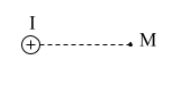
\includegraphics[scale=1]{../figs/VN11-2021-PH-TP021-01.JPG}
		\end{center}
		\begin{enumerate}[label=\alph*)]
			\item Hỏi điểm M cách dây một khoảng là bao nhiêu? 
			\item Biểu diễn vectơ cảm ứng từ tại điểm M.
		\end{enumerate}
		
	}
	
	\loigiai{
		
		\begin{enumerate}[label=\alph*)]
			\item  Khoảng cách từ M đến dây 
			
			$$B = 2 \cdot 10^{-7} \dfrac{I}{r} \Rightarrow r = \SI{0,05}{m}.$$
			
			\item Biểu diễn vectơ cảm ứng từ tại điểm M.
			\begin{center}
				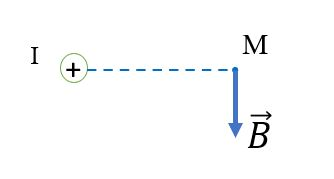
\includegraphics[scale=0.8]{../figs/VN11-2021-PH-TP021-05.JPG}
			\end{center}
			
		\end{enumerate}
	
	}
	
	

	
	\item \mkstar{3} [13]
	
	\cauhoi{
		\begin{minipage}[l]{12cm}
			Hai dây dẫn thẳng song song dài vô hạn đặt cách nhau một khoảng $\SI{14}{cm}$ trong không khí. Dòng điện chạy trong hai dây cùng chiều và có cường độ $I_1 = I_2 = \SI{2,5}{A}$. Đường thẳng CH nằm trong mặt phẳng vuông góc với mặt phẳng chứa hai dây dẫn và là đường trung trực của $I_1I_2$ (như hình vẽ) với  $\text{CH} = \SI{24}{cm}$.  Hãy vẽ vectơ cảm ứng từ tổng hợp tại C và tính độ lớn cảm ứng từ tổng hợp tại C.
		\end{minipage}
		\begin{minipage}[r]{5cm}
			\begin{center}
				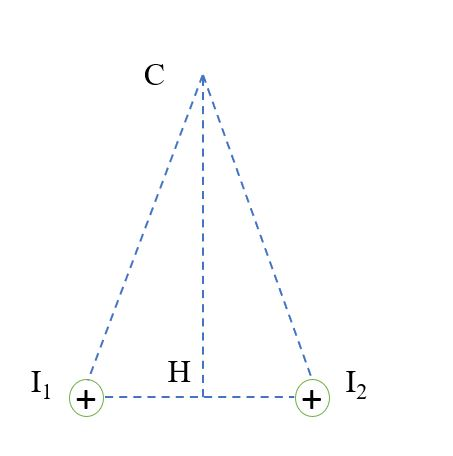
\includegraphics[scale=0.6]{../figs/VN11-2021-PH-TP021-02.JPG}
			\end{center}
		\end{minipage}
		
	}
	
	\loigiai{
		
		\begin{center}
			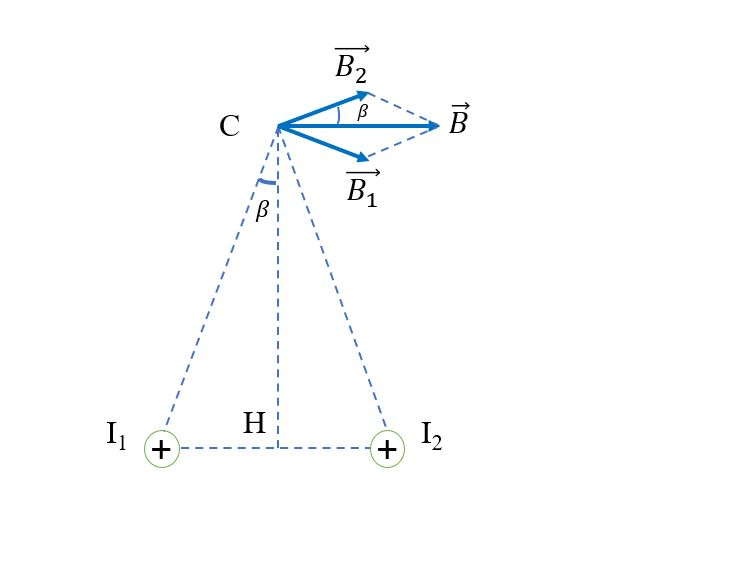
\includegraphics[scale=0.7]{../figs/VN11-2021-PH-TP021-03.JPG}
		\end{center}
		
		Ta có: $$ \vec B = \vec B_1 + \vec B_2.$$
		
		Do C là trung điểm của $I_1I_2$.
		
		Cảm ứng từ của $I_1$ và $I_2$ 
		
		$$B_1=B_2 = 2\cdot 10^{-7} \dfrac{I_1}{r_1} = 2 \cdot 10^{-6}\ \text{T}.$$
		
		Lại có: 
		
		$$\cos \beta = \dfrac{\text{CH}}{I_1\text{C}}.$$
		
		Cảm ứng từ tổng hợp 
		
		$$B=2B_1 \cos \beta= 3,84 \cdot 10^{-6}\ \text T.$$
		
	}
	\item \mkstar{3} [25]
	
	\cauhoi{
		
		Hai dây dẫn thẳng song song dài vô hạn đặt cách nhau $\SI{4}{cm}$ trong không khí. Dòng điện chạy trong hai dây là $I_1=\SI{10}{A}$; $I_2=\SI{20}{A}$ và ngược chiều nhau. Xác định hướng và độ lớn cảm ứng từ tại điểm M cách mỗi dây là $\SI{2}{cm}$.
		
		
	}
	\loigiai{
		
		\begin{center}
			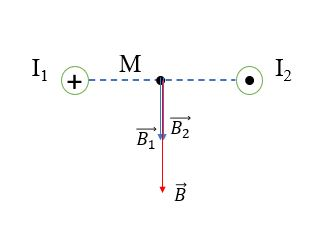
\includegraphics[scale=0.9]{../figs/VN11-2021-PH-TP021-04.JPG}
		\end{center}
		
		Cảm ứng từ của $I_1$ tác dụng lên M
		
		$$B_1 = 2 \cdot 10^{-7} \dfrac{I_1}{r_1} = 10^{-4}\ \text{T}.$$
		
		Cảm ứng từ của $I_2$ tác dụng lên M
		
		$$B_1 = 2 \cdot 10^{-7} \dfrac{I_1}{r_1} = 2 \cdot 10^{-4}\ \text{T}.$$
		
		Cảm ứng từ tổng hợp tại M
		
		$$ \vec B = \vec B_1 + \vec B_2$$
		
		Do $\vec B_1$ cùng hướng với $\vec B_2$ nên suy ra
		
		$$B = B_1+B_2 =3 \cdot 10^{-4}\ \text T.$$
		}
	
\end{enumerate}
\section{Lý thuyết: Từ trường do dòng điện chạy trong khung dây dẫn tròn hoặc trong ống dây hình trụ gây ra}
\begin{enumerate}[label=\bfseries Câu \arabic*:]
	
	\item \mkstar{2}
	
	\cauhoi{
		
		Khi cho dòng điện cường độ $\SI{10}{A}$ chạy qua một vòng dây dẫn đặt trong không khí thì cảm ứng từ tại tâm của vòng dây dẫn có độ lớn là $\text{2,1}\cdot 10^{-4}\ \text{T}$. Xác định bán kính của vòng dây.
		\begin{mcq}(4)
			\item $\SI{5,0}{cm}.$
			\item $\SI{0,3}{cm}.$
			\item $\SI{3,0}{cm}.$
			\item $\SI{2,5}{cm}.$
		\end{mcq}
	}
	\loigiai{
		
		\textbf{Đáp án: C.}
		
		Bán kính vòng dây  
		
		$$B = 2 \pi \cdot 10^{-7} \dfrac{I}{R} \Rightarrow R =  2 \pi \cdot 10^{-7} \dfrac{I}{B} = \SI{0,03}{m}.$$
	}	
	
	
	
		\item \mkstar{2}
		\cauhoi{
			
			Một vòng dây tròn đặt trong chân không có bán kính $R$ mang dòng điện có cường độ $I$ thì cảm ứng từ tại tâm vòng dây là $10\ \mu \text{T}$. Nếu cho dòng điện trên qua vòng dây có bán kính $4R$ thì cảm ứng từ tại tâm vòng dây có độ lớn là
			\begin{mcq}(4)
				\item $6 \cdot 10^{-6}\ \text{T}$.
				\item $\text{1,2}\cdot 10^{-6}\ \text{T}.$	
				\item $15 \cdot 10^{-6}\ \text{T}$.		
				\item $\text{2,5}\cdot 10^{-6}\ \text{T}.$	
			\end{mcq}
		}
		\loigiai{
			
			\textbf{Đáp án: D.}
			
			Ta có: 
			
			$$\dfrac{B_1}{B_2}= \dfrac{4R}{R} \Rightarrow B_2 = \dfrac{B_1}{4} =\text{2,5}\cdot 10^{-6}\ \text T. $$
		}	
	
		\item \mkstar{3}
		\cauhoi{
			
			Dùng một dây đồng có phủ một lớp sơn cách điện mỏng, quấn quanh một hình trụ dài $L = 50\ \text{cm}$, có đường kính $d = 4\ \text{cm}$ để làm một ống dây. Sợi dây quấn ống dây có chiều dài $l = 314\ \text{cm}$ và các vòng dây được quấn sát nhau. Hỏi nếu cho dòng điện cường độ $I = \text{0,4}\ \text{A}$ chạy qua ống dây, thì cảm ứng từ bên trong ống dây bằng bao nhiêu?
			\begin{mcq}(4)
				\item $5 \cdot 10^{-5}\ \text{T}$.			
				\item $\text{2,5}\cdot 10^{-5}\ \text{T}.$		
				\item $\text{1,25}\cdot 10^{-5}\ \text{T}.$		
				\item $3 \cdot 10^{-5}\ \text{T}$.	
			\end{mcq}
		}
		\loigiai{
			
			\textbf{Đáp án: B.}
			
			Chu vi của mỗi vòng dây $\pi d$.
			
			Số vòng dây
			
			$$N = \dfrac{l}{\pi d}.$$
			
			Cảm ứng từ tại bên trong ống dây
			
			$$B = 4 \pi \cdot 10^{-7} \dfrac{NI}{L}= 4  \cdot 10^{-7} \dfrac{ lI}{Ld} = \text{2,5} \cdot 10^{-5}\ \text{T}.$$
		}	

	
		\item \mkstar{1} [19]
	
	\cauhoi{
		
		Nêu công thức tính cảm ứng từ tại tâm của một khung dây dẫn tròn đặt trong không khí (có chú thích các đại lượng trong công thức).
		
	}
	
	\loigiai{
		
		+ Biểu thức: $$B = 2\pi \cdot 10^{-7} N \dfrac{I}{R}$$
		
		$N$: số vòng dây của khung.
		
		$I$: cường độ dòng điện qua khung.
		
		$R$: bán kính khung dây.
		
	}
\end{enumerate}

\whiteBGstarEnd
\stopcontents[mychapters]
\setcounter{mychapter}{14}
\mychapter{Dòng điện trong chất khí}
\startcontents[mychapters]
\printcontents[mychapters]{}{0}{\setcounter{tocdepth}{1}}
\whiteBGstarBegin
\setcounter{section}{0}
\section{Lý thuyết: Lực Lo-ren-xơ }
\begin{enumerate}[label=\bfseries Câu \arabic*:]
	\item \mkstar{2} 
	
	\cauhoi{
		Cho electron bay vào miền có từ trường đều với vận tốc $v = 8\cdot 10^5\ \text{m/s}$ theo phương vuông góc với vectơ cảm ứng từ, độ lớn cảm ứng từ là $B = \text{9,1}\cdot 10^{-4}\ \text{T}$. Tính độ lớn lực Lo-ren-xơ tác dụng lên electron.
		\begin{mcq}(2)
			\item $\text{1,1648}\cdot 10^{-16}\ \text{N}$. 
			\item $\text{1,1648}\cdot 10^{-17}\ \text{N}$.
			\item $\text{1,1648}\cdot 10^{-19}\ \text{N}$.
			\item $\text{1,1648}\cdot 10^{-20}\ \text{N}$.
		\end{mcq}
	}
	
	\loigiai{
		\textbf{Đáp án: A.}
		
		Góc hợp bởi $\vec B$ và $\vec v$ là $90^\circ$ nên ta có độ lớn của lực Lorenxo: 
		
		$$f = |e|vB \sin \alpha = 1,1648 \cdot 10^{-16}\ \text N.$$
		
	}
	\item \mkstar{2} 
	
	\cauhoi{
		Một hạt mang điện $\text{3,2}\cdot 10^{-19}\ \text{C}$ bay vào trong từ trường đều có $B = \text{0,5}\ \text{T}$ hợp với hướng của đường sức từ $30^\circ$. Lực Lorenxơ tác dụng lên hạt có độ lớn $\text{8}\cdot 10^{-14}\ \text{N}$. Vận tốc của hạt đó khi bắt đầu vào trong từ trường là bao nhiêu?
		\begin{mcq}(2)
			\item $v = 2\cdot 10^6\ \text{m/s}$.
			\item $v = 1\cdot 10^6\ \text{m/s}$.
			\item $v = 3\cdot 10^6\ \text{m/s}$.
			\item $v = 5\cdot 10^6\ \text{m/s}$.
		\end{mcq}
		
	}
	
	\loigiai{
		\textbf{Đáp án: B.}
		
		Vận tốc của hạt đó khi bắt đầu vào trong từ trường 
		
		$$f =qvB \sin  \alpha \Rightarrow v = \dfrac{F}{|q| B \sin \alpha} = 10^6\ \text{m/s}.$$
	}
	
		\item \mkstar{3} 
	
	\cauhoi{
		Một hạt điện tích chuyên động trong từ trường đều quĩ đạo của hạt vuông góc với đường sức từ. Nếu hạt chuyển động với vận tốc $v_1=\text{1,8}\cdot 10^{6}\ \text{m/s}$ thì lực Lo-ren-xơ tác dụng lên hạt có độ lớn là $f_1=\text{2}\cdot 10^{-6}\ \text{N}$, nếu hạt chuyển động với vận tốc là $v_1=\text{4,5}\cdot 10^{7}\ \text{m/s}$ thì lực Loren tác dụng lên hạt có giá trị là
		\begin{mcq}(2)
			\item $f_2=\text{2}\cdot 10^{-5}\ \text{N}$. 
			\item $f_2=\text{3}\cdot 10^{-5}\ \text{N}$.
			\item $f_2=\text{5}\cdot 10^{-5}\ \text{N}$.
			\item $f_2=\text{6}\cdot 10^{-5}\ \text{N}$.
		\end{mcq}
	}
	
	\loigiai{
		\textbf{Đáp án: C.}
		
		Một hạt tích điện chuyển động trong từ trường đều, lực Lorenxo tác dụng lên hạt 
		
		$$f_1 = qvB_1.$$ 
		
		$$f_2 = qvB_2.$$
		
		Ta có: 
		
		$$\dfrac{f_2}{f_1} = \dfrac{v_2}{v_1} \Leftrightarrow \dfrac{f_2}{2 \cdot 10^{-6}} = \dfrac{4,5 \cdot 10^7}{1,8 \cdot 10^6} \Rightarrow f_2 = 5 \cdot 10^{-5}\ \text{N}.$$
			
	}
	
	
\end{enumerate}
\section{Lý thuyết: Chuyển động của hạt mang điện trong từ trường đều (đọc thêm)}
\begin{enumerate}[label=\bfseries Câu \arabic*:]
		\item \mkstar{2}
	
	\cauhoi{
		Một ion bay theo quỹ đạo hòn bán kính $R$ trong một mặt phẳng vuông góc với các đường sức của một từ trường đều. Khi độ lớn vận tốc tăng gấp đôi thì bán kính quỹ đạo là 
		\begin{mcq}(4)
			\item $\dfrac{R}{2}.$ 
			\item $\dfrac{R}{4}.$
			\item $2R.$
			\item $4R.$
		\end{mcq}
		
	}
	
	\loigiai{
		\textbf{Đáp án: C.}
		
		Bán kính quỹ đạo của ion chuyển động trong từ trường khi có vận tốc vuông góc với đường sức từ là: 
		
		$$R = \dfrac{mv}{|q|B}.$$
		
		Vậy khi vận tốc tăng lên gấp đôi thì bán kính cũng tăng lên 2 lần.
	}
	
	\item \mkstar{3}
	\cauhoi{
		Hạt electron với vận tốc đầu bằng không được gia tốc qua một hiệu điện thế $\SI{400}{V}$. Tiếp đó nó được dẫn vào miền có từ trường đều vuông góc hướng chuyển động. Quỹ đạo của electron là đường tròn bán kính $R = \SI{7}{cm}$. Xác định độ lớn cảm ứng từ $B$.
		\begin{mcq}(2)
			\item $\text{9,636}\cdot 10^{-4}\ \text{T}$.
			\item $\text{4,818}\cdot 10^{-4}\ \text{T}$.
			\item $\text{3,212}\cdot 10^{-4}\ \text{T}$.
			\item $\text{6,242}\cdot 10^{-4}\ \text{T}$.
		\end{mcq}
	}
	
	\loigiai{
		\textbf{Đáp án: A.}
		
		Độ biến thiên động năng bằng công ngoại lực.
		
		Vận tốc của electron thu được khi tăng tốc bằng hiệu điện thế $U$ là
		
		$$\dfrac{1}{2} m_e v^2 =|e|U \Rightarrow v = 1,186 \cdot 10^7\ \text{m/s}.$$
		
		Khi electron đi vào từ trường đều, lực Lorenxo đóng vai trò là lực hướng tâm 
		
		$$|e| vB = \dfrac{m_e v^2}{r} \Rightarrow B = 9,636 \cdot 10^{-4}\ \text{T}.$$
	}


\end{enumerate}

\whiteBGstarEnd
\stopcontents[mychapters]
\setcounter{mychapter}{16}
\mychapter{Dòng điện trong chất bán dẫn}
\startcontents[mychapters]
\printcontents[mychapters]{}{0}{\setcounter{tocdepth}{1}}
\whiteBGstarBegin
\setcounter{section}{0}
\section{Trắc nghiệm}
\begin{enumerate}[label=\bfseries Câu \arabic*:]
	
	
	\item \mkstar{1}
	
	\cauhoi
	{Người ta gọi silic là chất bán dẫn vì
		\begin{mcq}
			\item nó không phải là kim loại, cũng không phải là điện môi.
			\item hạt tải điện trong đó có thể là electron và lỗ trống.
			\item điện trở suất của nó rất nhạy với nhiệt độ, tạp chất và các tác nhân ion khác.
			\item Cả 3 lí do trên.
		\end{mcq}
		
	}
	\loigiai
	{	\textbf{Đáp án: D.}
		
	}
	\item \mkstar{1}
	
	\cauhoi
	{Phát biểu nào dưới dây về transistor là chính xác?
		\begin{mcq}
			\item Một bán dẫn loại p kẹp giữa hai lớp bán dẫn loại n là transistor n-p-n.
			\item Một bán dẫn loại n mỏng kẹp giữa hai lớp bán dẫn loại p không thể xem là transistor.
			\item Một lớp bán dẫn loại p mỏng kẹp giữa hai lớp bán dẫn loại n luôn có khả năng là mạch khuếch đại.
			\item Trong transistor n-p-n, bao giờ mật độ hạt tải điện vùng Emitor cũng cao hơn vùng Base.
		\end{mcq}
		
	}
	\loigiai
	{	\textbf{Đáp án: D.}
	
	}
	\item \mkstar{1}
	
	\cauhoi
	{Silic tinh khiết thì
		\begin{mcq}
			\item dẫn điện tốt ở moi nhiệt độ.
			\item chỉ dẫn điện tốt khi ở nhiệt độ thấp.
			\item có liên kết đồng hóa trị giữa hai nguyên tử.
			\item chỉ có một loại hạt tải điện là electron.
		\end{mcq}
		
	}
	\loigiai
	{	\textbf{Đáp án: C.}
		
	}
	\item \mkstar{1}
	
	\cauhoi
	{Pin mặt trời là một nguồn điện biến đổi năng lượng từ
		\begin{mcq}(2)
			\item nhiệt năng thành điện năng.
			\item quang năng thành điện năng.
			\item cơ năng thành điện năng.
			\item hóa năng thành điện năng.
		\end{mcq}
		
	}
	\loigiai
	{	\textbf{Đáp án: B.}
		
	}
	\item \mkstar{1}
	
	\cauhoi
	{Lớp tiếp giáp p-n có
		\begin{mcq}
			\item tác dụng ngăn cản các electron từ p sang n.
			\item tác dụng ngăn cản các electron từ n sang p.
			\item tính dẫn điện một chiều từ n sang p.
			\item tính dẫn điện một chiều từ p sang n.
		\end{mcq}
		
	}
	\loigiai
	{	\textbf{Đáp án: C.}
		
	}
	\item \mkstar{1}
	
	\cauhoi
	{Cách pha tạp nào sau đây tạo ra bán dẫn loại p?
		\begin{mcq}(2)
			\item Si pha tạp As.
			\item Si pha tạp B.
			\item Si pha tạp S.
			\item Si pha tạp Pb.
		\end{mcq}
		
	}
	\loigiai
	{	\textbf{Đáp án: B.}
		
	}
	\item \mkstar{1}
	
	\cauhoi
	{Hạt mang điện chủ yếu trong bán dẫn loại n là
		\begin{mcq}(2)
			\item lỗ trống.
			\item electron.
			\item electron và lỗ trống.
			\item electron và ion dương.
		\end{mcq}
		
	}
	\loigiai
	{	\textbf{Đáp án: B.}
		
	}
	\item \mkstar{1}
	
	\cauhoi
	{Chọn câu đúng. Diode bán dẫn được dùng để
		\begin{mcq}
			\item nấu chảy kim loại.
			\item chỉnhh lưu dòng điện xoay chiều.
			\item tạo ra dòng điện xoay chiều.
			\item biến đổi dòng điện một chiều thành dòng điện xoay chiều.
		\end{mcq}
		
	}
	\loigiai
	{	\textbf{Đáp án: B.}
		
	}
	\item \mkstar{1}
	
	\cauhoi
	{Bán dẫn chứa tạp chất nhận là bán dẫn có đặc điểm:
		\begin{mcq}
			\item có mật độ lỗ trống rất lớn so với mật độ electron.
			\item có mật độ electron rất lớn so với mật độ lỗ trống.
			\item chỉ có một loại hạt tải điện là lỗ trống.
			\item chỉ có một loại hạt tải điện là electron.
		\end{mcq}
		
	}
	\loigiai
	{	\textbf{Đáp án: A.}
		
	}
	\item \mkstar{1}
	
	\cauhoi
	{Transistor là dụng cụ bán dẫn có số lớp chuyển tiếp p-n trong nó là
		\begin{mcq}(4)
			\item 4 lớp.
			\item 2 lớp.
			\item 3 lớp .
			\item 1 lớp.
		\end{mcq}
		
	}
	\loigiai
	{	\textbf{Đáp án: B.}
		
	}

\end{enumerate}

\whiteBGstarEnd

\loigiai
{
	\begin{center}
		\textbf{BẢNG ĐÁP ÁN}
	\end{center}
	\begin{center}
		\begin{tabular}{|m{2.8em}|m{2.8em}|m{2.8em}|m{2.8em}|m{2.8em}|m{2.8em}|m{2.8em}|m{2.8em}|m{2.8em}|m{2.8em}|}
			\hline
			1.D  & 2.D  & 3.C  & 4.B  & 5.C  & 6.B  & 7.B  & 8.B  & 9.A  & 10.B  \\
			\hline
			
		\end{tabular}
	\end{center}
}
\section{Tự luận}
\begin{enumerate}[label=\bfseries Câu \arabic*:]
	\item \mkstar{1}
	
	\cauhoi{
		Chất bán dẫn là gì? Nêu bản chất dòng điện trong chất bán dẫn.
	}
	
	\loigiai{
		
		Chất bán dẫn là chất có điện trở suất nằm trong khoảng trung gian giữa kim loại và chất điện môi.
		
		Dòng điện trong chất bán dẫn là dòng các electron dẫn chuyển động ngược chiều điện trường và dòng các lỗ trống chuyển động cùng chiều điện trường.
	}
	
	\item \mkstar{2}
	
	\cauhoi{
		So sánh chất bán dẫn loại n và loại p theo các tiêu chí được cho trong bảng sau:
		\begin{longtable}{|m{8em}|m{14em}|m{14em}|}
			\hline
			& \thead{Bán dẫn loại n} & \thead{Bán dẫn loại p} \\
			\hline
			\textbf{Định nghĩa} & & \\
			\hline
			\textbf{Hạt tải đa số} & & \\
			\hline
			\textbf{Tạp chất} & & \\
			\hline
		\end{longtable}
	}
	
	\loigiai{
		
		\begin{longtable}{|m{8em}|m{14em}|m{14em}|}
			\hline
			& \thead{Bán dẫn loại n} & \thead{Bán dẫn loại p} \\
			\hline
			\textbf{Định nghĩa} & Là chất bán dẫn mà hạt tải điện đa số trong đó mang điện âm. & Là chất bán dẫn mà hạt tải điện đa số trong đó mang điện dương.\\
			\hline
			\textbf{Hạt tải đa số} & Các electron. & Các lỗ trống. \\
			\hline
			\textbf{Tạp chất} & Tạp chất cho (donor): Sinh ra electron dẫn, thường là những nguyên tố có 5 electron hóa trị như $\ce{P}$, $\ce{As}$, $\ldots$. & Tạp chất nhận (aceptor): Nhận electron (đồng nghĩa sinh ra lỗ trống), thường là những nguyên tố có 5 electron hóa trị như $\ce{B}$, $\ce{Al}$, $\ldots$.\\
			\hline
		\end{longtable}
	}
	\item \mkstar{3}
	
	\cauhoi{
		Ở nhiệt độ phòng, trong bán dẫn Si tinh khiết có số cặp điện tử-lỗ trống bằng $\SI{e-13}{}$ lần số nguyên tử Si. Tìm số cặp điện tử-lỗ trống có trong $\SI{2}{mol}$ nguyên tử Si.
	}
	
	\loigiai{
		
		Số nguyên tử $\ce{Si}$ có trong $\SI{2}{\mol}$ là
		$$N = 2 N_\text{A} = \SI{1.205e24}{}.$$
		
		Số cặp điện tử-lỗ trống bằng $\SI{e-13}{}$ lần số nguyên tử, suy ra số cặp điện tử-lỗ trống là
		$$\SI{e-13}{} \cdot N = \SI{1.205e11}{}.$$
	}
	\item \mkstar{3}
	
	\cauhoi{
		Ở nhiệt độ phòng, trong bán dẫn Si tinh khiết có số cặp điện tử-lỗ trống bằng $\SI{e-13}{}$ lần số nguyên tử Si. Nếu pha P và Si với tỉ lệ một phần triệu thì số hạt tải điện tăng lên bao nhiêu lần?
	}
	
	\loigiai{
		
		Gọi $N_0$ là số nguyên tử $\ce{Si}$ có trong chất bán dẫn.
		
		Ở nhiệt độ phòng, trong bán dẫn $\ce{Si}$ tinh khiết, số cặp điện tử-lỗ trống bằng $\SI{e-13}{} N_0$. Tức là số hạt tải điện bằng:
		$$N=\SI{e-13}{} N_0.$$
		
		Khi pha một nguyên tử $\ce{P}$ vào bán dẫn $\ce{Si}$ tinh khiết sẽ tạo ra thêm 1 electron tự do. Với tỉ lệ pha tạp là một phần triệu thì số hạt tải điện tăng thêm là
		$$\Delta N = \SI{e-6}{} N_0.$$
		
		Vậy số hạt tại điện tăng thêm gấp $\dfrac{\Delta N}{N} = \SI{5e6}{}$ lần.
	}
	
\end{enumerate}
\stopcontents[mychapters]
\chapter{Ôn tập: Chương III. Dòng điện trong các môi trường}
\startcontents[mychapters]
\printcontents[mychapters]{}{0}{\setcounter{tocdepth}{1}}
\whiteBGstarBegin
\setcounter{section}{0}
\section{Trắc nghiệm}
\begin{enumerate}[label=\bfseries Câu \arabic*:]
	
	
	\item \mkstar{1}
	
	\cauhoi
	{Câu nào dưới đây nói về chất điện phân là \textbf{không} đúng?
		\begin{mcq}
			\item Chất điện phân khi có dòng điện chạy qua sẽ giải phóng các chất ở các điện cực.
			\item Trong dung dịch, các phân tử axit, muối, bazơ đều bị phân li thành các ion.
			\item Một số chất rắn khi nóng chảy cũng là chất điện phân.
			\item Chất điện phân nhất thiết phải là dung dịch của các chất tan được trong dung môi.
		\end{mcq}
		
	}
	\loigiai
	{	\textbf{Đáp án: D.}
		
		Chất điện phân không nhất thiết phải là dung dịch của các chất tan được trong dung môi.
	}
	\item \mkstar{1}

\cauhoi
{Câu nào sau đây khi nói về dòng điện trong chất điện phân là đúng?
	\begin{mcq}
		\item Khi có dòng điện chạy qua bình điện phân thì các electron và ion âm đi về phía anode, còn các ion dương đi về cathode.
		\item Khi có dòng điện chạy qua bình điện phân thì các electron đi về phía anode, các ion dương đi về cathode.
		\item Khi có dòng điện chạy qua bình điện phân thì các ion âm đi về phía anode, các ion dương đi về cathode.
		\item Khi có dòng điện chạy qua bình điện phân thì các ion âm và electron đi về phía cathode, các ion dương đi về anode.
	\end{mcq}
	
}
\loigiai
{	\textbf{Đáp án: C.}
	
	Khi có dòng điện chạy qua bình điện phân thì các ion âm đi về phía anode, các ion dương đi về cathode.
}
	\item \mkstar{1}

\cauhoi
{Câu phát biểu nào sau đây \textbf{sai}?
	\begin{mcq}
		\item Dòng điện trong kim loại là dòng chuyển dời có hướng của các electron ngược chiều điện trường.
		\item Dòng điện trong chất điện phân là dòng chuyển dời có hướng của các ion dương theo chiều điện trường, của các ion âm ngược chiều điện trường.
		\item Dòng điện trong chất khí là dòng chuyển dời có hướng của các ion dương theo chiều điện trường, của các ion âm ngược chiều điện trường.
		\item Dòng điện trong chân không là dòng chuyển dời có hướng của các electron phát xạ từ cathode bị nung nóng dưới tác dụng của điện trường.
	\end{mcq}
	
}
\loigiai
{	\textbf{Đáp án: C.}
	
	Dòng điện trong chất khí là dòng chuyển dời có hướng của các ion dương theo chiều điện trường, của các ion âm và các electron ngược chiều điện trường. Các hạt tải điện này là do chất khí bị ion hóa sinh ra.
}
	\item \mkstar{1}

\cauhoi
{Câu nào sau đây \textbf{sai} khi nói về tính dẫn điện của chất điện phân?
	\begin{mcq}
		\item Dòng điện trong chất điện phân tuân theo định luật Ôm.
		\item Độ dẫn điện của chất điện phân tăng khi nhiệt độ tăng.
		\item Điện trở của chất điện phân giảm khi nhiệt độ tăng.
		\item Khi ắc quy được nạp điện, dòng điện qua ắc quy cũng là dòng điện trong chất điện phân.
	\end{mcq}
	
}
\loigiai
{	\textbf{Đáp án: A.}
	
	Dòng điện trong chất điện phân chỉ tuân theo định luật Ôm khi xảy ra hiện tượng dương cực tan.
}
	\item \mkstar{2}

\cauhoi
{Phát biểu nào sau đây là đúng?
	\begin{mcq}
		\item Dòng điện trong kim loại cũng như trong chân không đều là dòng chuyển động có hướng của các electron, ion dương và ion âm.
		\item Dòng điện trong kim loại là dòng chuyển động có hướng của các electron, dòng điện trong chân không và trong chất khí đều là dòng chuyển động có hướng của các ion dương và ion âm.
		\item Dòng điện trong kim loại và trong chân không đều là dòng chuyển động có hướng của các electron.
		\item Dòng điện trong kim loại và dòng điện trong chất khí là dòng chuyển động có hướng của các ion.
	\end{mcq}
	
}
\loigiai
{	\textbf{Đáp án: C.}
	
	Dòng điện trong kim loại và trong chân không đều là dòng chuyển động có hướng của các electron.
}
	\item \mkstar{2}

\cauhoi
{Nguyên nhân gây ra điện trở của kim loại là
	\begin{mcq}
		\item do sự va chạm của các electron với các ion dương ở các nút mạng.
		\item do sự va chạm của các ion dương ở các nút mạng với nhau.
		\item do sự va chạm của các electron với nhau.
		\item Cả B và C đều đúng.
	\end{mcq}
	
}
\loigiai
{	\textbf{Đáp án: A.}
	
	Nguyên nhân gây ra điện trở của kim loại là do sự va chạm của các electron với các ion dương ở các nút mạng.
}
	\item \mkstar{2}

\cauhoi
{Phát biểu nào dưới đây về sự phụ thuộc của cường độ dòng điện $I$ vào hiệu điện thế $U$ giữa hai cực tụ điện chứa chất khí trong quá trình dẫn điện không tự lực là \textbf{không} đúng?
	\begin{mcq}
		\item Với mọi giá trị của $U$, $I$ luôn tăng tỉ lệ với $U$.
		\item Với $U$ nhỏ, $I$ tăng theo $U$.
		\item Với $U$ đủ lớn, $I$ đạt giá trị bão hòa.
		\item Với $U$ quá lớn, $I$ tăng nhanh theo $U$.
	\end{mcq}
	
}
\loigiai
{	\textbf{Đáp án: A.}
	
	Dòng điện $I$ tỉ lệ với $U$ đến khi $I$ đạt bão hòa thì $I$ không tăng nữa. Khi đó $I$ không còn tỉ lệ với $U$.
}
	\item \mkstar{2}

\cauhoi
{Hai thanh kim loại được nối với nhau bởi hai đầu mối hàn tạo thành một mạch kín, hiện tượng nhiệt điện chỉ xảy ra khi
	\begin{mcq}
		\item hai thanh kim loại có bản chất khác nhau và nhiệt độ ở hai đầu mối hàn bằng nhau.
		\item hai thanh kim loại có bản chất khác nhau và nhiệt độ ở hai đầu mối hàn khác nhau.
		\item hai thanh kim loại có bản chất giống nhau và nhiệt độ ở hai đầu mối hàn bằng nhau.
		\item hai thanh kim loại có bản chất giống nhau và nhiệt độ ở hai đầu mối hàn khác nhau.
	\end{mcq}
	
}
\loigiai
{	\textbf{Đáp án: B.}
	
	Hai thanh kim loại được nối với nhau bởi hai đầu mối hàn tạo thành một mạch kín, hiện tượng nhiệt điện chỉ xảy ra khi hai thanh kim loại có bản chất khác nhau và nhiệt độ ở hai đầu mối hàn khác nhau.
}
	\item \mkstar{2}

\cauhoi
{Khi cho dòng điện chạy qua một sợi dây thép có hệ số nhiệt điện trở là $\SI{0.004}{K^{-1}}$ thì điện trở của nó tăng gấp đôi. Nhiệt độ của sợi dây này đã tăng thêm
	\begin{mcq}(4)
		\item $\SI{800}{\celsius}$.
		\item $\SI{250}{\celsius}$.
		\item $\SI{300}{\celsius}$.
		\item $\SI{80}{\celsius}$.
	\end{mcq}
	
}
\loigiai
{	\textbf{Đáp án: B.}
	
	Áp dụng công thức:
	$$R=R_0 [1+ \alpha (t-t_0)] \Rightarrow t-t_0 = \SI{250}{\celsius}.$$
}
	\item \mkstar{2}

\cauhoi
{Ở $\SI{20}{\celsius}$, điện trở suất của bạc là $\SI{1.62e-8}{\Omega m}$. Biết hệ số nhiệt điện trở của bạc là $\SI{4.1e-3}{K^{-1}}$. Ở $\SI{330}{K}$ thì điện trở suất của bạc là
	\begin{mcq}(2)
		\item $\SI{1.866e-8}{\Omega m}$.
		\item $\SI{3.679e-8}{\Omega m}$.
		\item $\SI{3.812e-8}{\Omega m}$.
		\item $\SI{4.151e-8}{\Omega m}$.
	\end{mcq}
	
}
\loigiai
{	\textbf{Đáp án: A.}
	
	Ta có $t-t_0 = \SI{330}{K} - \SI{293}{K} = \SI{37}{K}$.
	
	Áp dụng công thức:
	$$\rho = \rho_0 [1+ \alpha (t-t_0)] = \SI{1.866e-8}{\Omega m}.$$
}
	
\end{enumerate}

\whiteBGstarEnd

\loigiai
{
	\begin{center}
		\textbf{BẢNG ĐÁP ÁN}
	\end{center}
	\begin{center}
		\begin{tabular}{|m{2.8em}|m{2.8em}|m{2.8em}|m{2.8em}|m{2.8em}|m{2.8em}|m{2.8em}|m{2.8em}|m{2.8em}|m{2.8em}|}
			\hline
			1.D  & 2.C  & 3.C  & 4.A  & 5.C  & 6.A  & 7.A  & 8.B  & 9.B  & 10.A  \\
			\hline
			
		\end{tabular}
	\end{center}
}
\section{Tự luận}
\begin{enumerate}[label=\bfseries Câu \arabic*:]
	\item \mkstar{2}
	
	\cauhoi{
	Một sợi dây đồng có điện trở $\SI{74}{\Omega}$ ở $\SI{50}{\celsius}$, có hệ số nhiệt điện trở là $\SI{4.1e-3}{K^{-1}}$. Tính điện trở của sợi dây đó ở $\SI{100}{\celsius}$.
	}
	
	\loigiai{
		
		Điện trở của sợi dây ở $\SI{100}{\celsius}$:
		$$\dfrac{R_2}{R_1} = \dfrac{1 + \alpha t_2}{1+ \alpha t_1} \Rightarrow R_2 = \SI{86.6}{\Omega}.$$
	}
	
	\item \mkstar{2}
	
	\cauhoi{
		Một mối hàn của một cặp nhiệt điện có hệ số $\alpha_T = \SI{48}{\micro V / K}$ được đặt trong không khí ở $\SI{20}{\celsius}$, còn mối hàn kia được nung nóng đến nhiệt độ $t \SI{}{\celsius}$, suất điện động của cặp nhiệt điện khi đó là $\calE = \SI{6}{mV}$. Xác định nhiệt độ của mối hàn còn lại.
	}
	
	\loigiai{
		
		Áp dụng công thức tính suất điện động nhiệt điện:
		$$\calE = \alpha_T (T_1 - T_2) \Rightarrow T_1 = \SI{418}{K} \Rightarrow t_1 = \SI{145}{\celsius}.$$
	}
	\item \mkstar{2}
	
	\cauhoi{
		Một bình điện phân chứa dung dịch bạc nitrate có điện trở là $\SI{5}{\Omega}$. Anode của bình bằng bạc và hiệu điện thế đặt vào hai điện cực của bình là $\SI{20}{V}$. Tính khối lượng bạc bám vào cathode sau 32 phút 10 giây.
	}
	
	\loigiai{
		
		Cường độ dòng điện qua bình điện phân:
		$$I=\dfrac{U}{R} = \SI{4}{A}.$$
		
		Áp dụng định luật Fa-ra-đây để tính khối lượng bạc bám vào cathode:
		$$m=\dfrac{1}{F} \dfrac{A}{n} I t = \SI{8.64}{g}.$$
	}
	\item \mkstar{3}
	
	\cauhoi{
		Để giải phóng lượng $\ce{Cl}$ và $\ce{H}$ từ $\SI{7.6}{g}$ $\ce{HCl}$ bằng dòng điện $\SI{5}{A}$ thì phải cần thời gian điện phân là bao lâu? Biết rằng đương lượng điện của $\ce{H}$ và $\ce{Cl}$ lần lượt là $k_1=\SI{0.1045e-7}{kg/C}$ và $k_2 = \SI{3.6e-7}{kg/C}$.
	}
	
	\loigiai{
		
		Áp dụng định luật Fa-ra-đây:
		$$m=(k_1 + k_2) It$$
		
		Suy ra thời gian cần phải điện phân là
		$$t=\SI{4027}{s} \approx \SI{1.1}{h}.$$
	}
	
\end{enumerate}
\stopcontents[mychapters]
\chapter{Pre-course: Chuyển động thẳng đều - Chuyển động thẳng biến đổi đều}
\whiteBGstarBegin
\begin{enumerate}[label=\bfseries Câu \arabic*:]
	
	\item \mkstar{1}
	
	\cauhoi
	{Chuyển động thẳng đều là
		\begin{mcq}
			\item chuyển động thẳng, trong đó chất điểm có gia tốc không đổi.
			\item chuyển động có quỹ đạo là đường thẳng và có gia tốc như nhau trên mọi quãng đường.
			\item chuyển động có quỹ đạo là đường thẳng và có tốc độ trung bình như nhau trên mọi quãng đường.
			\item chuyển động thẳng, trong đó chất điểm có vận tốc tức thời thay đổi.
		\end{mcq}
	}
	
	\loigiai
	{\textbf{Đáp án: C.}
		
		Chuyển động thẳng đều là chuyển động có quỹ đạo là đường thẳng và có tốc độ trung bình như nhau trên mọi quãng đường.
		
		
	}
	\item \mkstar{1}
	
	\cauhoi
	{Phương trình chuyển động của chuyển động thẳng chậm dần đều là
		\begin{mcq}
			\item $x=x_0+v_0t +\dfrac{at^2}{2}$ ($a$ và $v_0$ trái dấu).
			\item $s=v_0t+\dfrac{at^2}{2}$ ($a$ và $v_0$ trái dấu).
			\item $x=x_0+v_0t +\dfrac{at^2}{2}$ ($a$ và $v_0$ cùng dấu).
			\item $s=v_0t+\dfrac{at^2}{2}$ ($a$ và $v_0$ cùng dấu).
		\end{mcq}
	}
	\loigiai
	{\textbf{Đáp án: A.}
		
		Phương trình chuyển động của chuyển động thẳng chậm dần đều là
		$$x=x_0+v_0t +\dfrac{at^2}{2}\ (a \textrm{ và } v_0 \text{ trái dấu}).$$
		
		
	}
	\item \mkstar{1}
	
	\cauhoi
	{Chỉ ra câu \textbf{sai}.
		\begin{mcq}
			\item Gia tốc của chuyển động thẳng biến đổi đều có độ lớn không đổi. 
			\item Trong chuyển động thẳng biến đổi đều, quãng đường đi được trong những khoảng thời gian bằng nhau thì bằng nhau.
			\item Vận tốc tức thời của chuyển động thẳng biến đổi đều có độ lớn tăng hoặc giảm đều theo thời gian.
			\item Vectơ gia tốc của chuyển động thẳng biến đổi đều có thể cùng chiều hoặc ngược chiều với vectơ vận tốc.
		\end{mcq}
		
	}
	\loigiai
	{\textbf{Đáp án: B.}
		
		Công thức tính quãng đường đi được trong chuyển động thẳng biến đổi đều là
		$$s=v_0t+\dfrac{1}{2}at^2=\dfrac{1}{2}\left(v_0 + v_0+at \right) t=\dfrac{1}{2}\left(v_0+v\right) t\ (\text{với } v=v_0+at).$$
		
		Trong chuyển động biến đổi đều vận tốc $v$ thay đổi sau những khoảng thời gian bằng nhau, nên quãng đường đi được $s$ cũng thay đổi sau những khoảng thời gian bằng nhau.
		
		
	}
	\item \mkstar{2}
	
	\cauhoi
	{Phương trình chuyển động thẳng đều của một chất điểm có dạng $x=-4t+12$\\ ($x$: km, $t$: h). Quãng đường của chất điểm đi được sau $\SI{2}{\hour}$ là
		\begin{mcq}(4)
			\item $\SI{6}{\kilo\meter}$.
			\item $\SI{8}{\kilo\meter}$.
			\item $\SI{2}{\kilo\meter}$.
			\item $\SI{4}{\kilo\meter}$.
		\end{mcq}
	}
	\loigiai
	{\textbf{Đáp án: B.}	
		
		Quãng đường của chất điểm đi được sau $\SI{2}{\hour}$ là
		$$s=v_0t=\SI{4}{\kilo\meter/\hour}\cdot\SI{2}{\hour}=\SI{8}{\kilo\meter}.$$
		
		
	}
	\item \mkstar{2}
	
	\cauhoi
	{Một ôtô chuyển động trên một đoạn đường thẳng với tốc độ $\SI{60}{\kilo\meter/\hour}$. Bến xe nằm ở đầu đoạn đường nhưng xe xuất phát từ một điểm trên đoạn đường cách bến xe $\SI{4}{\kilo\meter}$. Chọn bến xe là vật mốc, chọn thời điểm xe xuất phát làm gốc thời gian và chọn chiều dương là chiều chuyển động. Phương trình chuyển động của ôtô trên đoạn đường này là
		\begin{mcq}(2)
			\item $x=60t$ (km, h).
			\item $x=4-60t$ (km, h).
			\item $x=4+60t$ (km, h).
			\item $x=-4-60t$ (km, h).
		\end{mcq}
		
	}
	\loigiai
	{\textbf{Đáp án: C.}
		
		Chọn bến xe là vật mốc, chọn thời điểm xe xuất phát làm gốc thời gian và chọn chiều dương là chiều chuyển động nên $x_0=\SI{4}{\kilo\meter}$, $v_0=\SI{60}{\kilo\meter/\hour}$.
		
		Phương trình chuyển động của ôtô trên đoạn đường này là: $x=4+60t$ (km, h).
		
		
	}
	\item \mkstar{2}
	
	\cauhoi{
		Trên trục $\text O x$ có hai ô tô chuyển động với phương trình tọa độ lần lượt là $x_1 (t) = -20t+100\ (\text {m; s})$ và $x_2 (t) = 10t-50\ (\text {m; s})$. Khoảng cách giữa hai ô tô lúc $t=2\ \text s$ là
		\begin{mcq}(4)
			\item $\SI{90}{\meter}$.
			\item $\SI{0}{\meter}$.
			\item $\SI{60}{\meter}$.
			\item $\SI{30}{\meter}$.
		\end{mcq}
	}
	\loigiai
	{\textbf{Đáp án: A.}
		
		Tại thời điểm $t=2\ \text s$ thì các ô tô có tọa độ là $x_1 = \SI{60}{\meter}$, $x_2 = \SI{-30}{\meter}$.
		
		Khoảng cách giữa hai ô tô lúc $t=2\ \text s$ là $\SI{90}{\meter}$.
		
		
	}
	\item \mkstar{2}
	
	\cauhoi{
		Lúc 7 giờ, một người ở A chuyển động thẳng đều với vận tốc $v=\SI{36}{\kilo \meter / \hour}$ đuổi theo người ở B đang chuyển động với vận tốc $v=\SI{5}{\meter / \second}$. Biết $\text{AB}=\SI{18}{\kilo \meter}$. Chọn gốc tọa độ ở A, chiều dương là chiều chuyển động. Phương trình chuyển động của người A và B lần lượt là
		\begin{mcq}(1)
			\item $x_\text A = 36t +18\ \text{(km, h)}$; $x_\text B = 18t\ \text{(km, h)}$.
			\item $x_\text A = 36t -18\ \text{(km, h)}$; $x_\text B = 18t + 18\ \text{(km, h)}$.
			\item $x_\text A = 36t\ \text{(km, h)}$; $x_\text B = 18t+18\ \text{(km, h)}$.
			\item $x_\text A = 36t\ \text{(km, h)}$; $x_\text B = 18t\ \text{(km, h)}$.
		\end{mcq}	
	}
	\loigiai
	{\textbf{Đáp án: C.}
		
		 Chọn gốc tọa độ ở A, chiều dương là chiều chuyển động.
		
		Phương trình chuyển động của người ở A: $x_\text A = 36t+0=36t\ \text{(km, h)}$.
		
		Phương trình chuyển động của người ở B (đổi $\SI{5}{\meter / \second} \rightarrow \SI{18}{\kilo \meter / \hour}$): $x_\text B = 18t+18\ \text{(km, h)} $.
		
		
	}
	\item \mkstar{2}
	
	\cauhoi{ Phương trình chuyển động của một vật trên một đường thẳng có dạng $x=2t^2 + 10t+100\ \text{(m; s)}$. Thông tin nào sau đây là đúng?
		\begin{mcq}(1)
			\item Vật chuyển động nhanh dần đều với gia tốc là $a=\SI{2}{\meter / \second \squared}$.
			\item Vật chuyển động chậm dần đều với gia tốc là $a=\SI{4}{\meter / \second \squared}$.
			\item Tọa độ của vật lúc $t=\SI{0}{\second}$ là $x=\SI{100}{\meter}$.
			\item Vận tốc của vật tại mọi thời điểm là $v=\SI{10}{\meter / \second}$.
		\end{mcq}
	}
	\loigiai
	{\textbf{Đáp án: C.}
		
		
		Phương trình chuyển động thẳng biến đổi đều: $x=\dfrac{1}{2}at^2+v_0t+x_0$.
		
		Ta thấy $a=\SI{4}{\meter / \second \squared}$, $v_0=\SI{10}{\meter / \second}$, $x_0=\SI{100}{\meter}$.
		
		Do $a$ và $v_0$ cùng dấu nên vật chuyển động nhanh dần đều với gia tốc $a=\SI{4}{\meter / \second \squared}$, thời điểm ban đầu ($t=\SI{0}{\second}$) vật có tọa độ $x=\SI{100}{\meter}$.
		
		
	}
	\item \mkstar{2}
	
	\cauhoi{Phương trình chuyển động của một vật trên một đường thẳng có dạng $x=4t^2-3t+3\ \text{(m; s)}$. Điều nào sau đây đúng?
		\begin{mcq}(1)
			\item Gia tốc của vật là $a=\SI{4}{\meter / \second \squared}$.
			\item Tọa độ của vật ở thời điểm ban đầu là $x_0=\SI{6}{\meter}$.
			\item Tọa độ của vật ở thời điểm $\SI{1}{\second}$ là $x=\SI{3}{\meter}$.
			\item Vận tốc ban đầu của vật là $v_0=\SI{-3}{\meter / \second}$.
		\end{mcq}
	}
	\loigiai
	{\textbf{Đáp án: D.}
		
		Phương trình chuyển động thẳng biến đổi đều: $x=\dfrac{1}{2}at^2+v_0t+x_0$.
		
		Ta thấy $a=\SI{8}{\meter / \second \squared}$, $v_0=\SI{-3}{\meter / \second}$, $x_0=\SI{3}{\meter}$.
		
		
	}
	\item \mkstar{2}
	
	\cauhoi{Một vật chuyển động thẳng chậm dần đều với tốc độ ban đầu $\SI{3}{\meter/\second}$ và gia tốc có độ lớn $\SI{2}{\meter/\second^2}$. Biết thời điểm ban đầu vật ở gốc tọa độ và chuyển động ngược chiều dương của trục tọa độ. Phương trình chuyển động của vật là
		\begin{mcq}(2)
			\item $x=-3t-t^2$ (m, s).
			\item $x=3t+t^2$ (m, s).
			\item $x=-3t-t^2$ (m, s).
			\item $x=-3t+t^2$ (m, s).
		\end{mcq}
	}
	\loigiai
	{\textbf{Đáp án: D.}
		
		Chọn gốc thời gian là khi vật bắt đầu chuyển động.
		
		Vì vật chuyển động chậm dần đều ngược chiều dương nên:
		\begin{equation*}
			\left\{\begin{array}{ll}{a\cdot v <0}&\\{v < 0}&\end{array}\right.\Rightarrow \left\{\begin{array}{ll}{a > 0}&\\{v < 0.}&\end{array}\right.
		\end{equation*}
		
		Kết hợp với các dữ kiện của đề bài, ta suy ra:
		\begin{equation*}
			\left\{\begin{array}{ll}{a=\SI{2}{\meter/\second^2}}&\\{v=\SI{-3}{\meter/\second} .}&\end{array}\right.
		\end{equation*}
		
		Phương trình chuyển động của vật có dạng:
		$x=-3t+t^2$ (m, s).
		
		
	}
	\item \mkstar{2}
	
	\cauhoi{Lúc $\SI{7}{\hour}$, hai ô tô bắt đầu khởi hành từ hai điểm A, B cách nhau $\SI{2400}{\meter}$, chuyển động nhanh dần đều và ngược chiều nhau. Ô tô đi từ A có gia tốc $\SI{1}{\meter / \second \squared}$, còn ô tô đi từ B có gia tốc $\SI{2}{\meter / \second \squared}$. Chọn chiều dương hướng từ A đến B, gốc thời gian lúc $\SI{7}{\hour}$. Xác định vị trí hai xe gặp nhau.
		\begin{mcq}(4)
			\item $\SI{1600}{\meter}$.
			\item $\SI{1200}{\meter}$.
			\item $\SI{800}{\meter}$.
			\item $\SI{2400}{\meter}$.
		\end{mcq}
	}
	\loigiai
	{\textbf{Đáp án: C.}
		
		Chọn chiều dương hướng từ A đến B, gốc thời gian lúc $\SI{7}{\hour}$.
		
		Phương trình chuyển động của xe A: $x_\text A = 0,5t^2$.
		
		Phương trình chuyển động của xe B: $x_\text B=-t^2 + 2400$.
		
		Hai xe gặp nhau: $x_\text A = x_\text B \Rightarrow t = \SI{40}{\second} \Rightarrow x=\SI{800}{\meter}$.
		
		
	}
	\item \mkstar{3}
	
	\cauhoi{Một xe chạy trong $\SI{5}{\hour}$, $\SI{2}{\hour}$ đầu xe chạy với tốc độ trung bình $\SI{60}{\km/\hour}$, $\SI{3}{\hour}$ sau xe chạy với tốc độ trung bình $\SI{40}{\km/\hour}$. Tốc độ trung bình của xe trong suốt thời gian chuyển động là
		\begin{mcq}(4)
			\item $\SI{48}{\kilo\meter/ \hour}$.
			\item $\SI{36}{\kilo\meter/ \hour}$.
			\item $\SI{54}{\kilo\meter/ \hour}$.
			\item $\SI{72}{\kilo\meter/ \hour}$.
		\end{mcq}
	}
	\loigiai
	{\textbf{Đáp án: A.}
		
		Quãng đường đi trong $\SI{2}{\hour}$ đầu là
		$$s_1 = v_1t_1 = \SI{60}{\km/\hour}\cdot\SI{2}{\hour} = \SI{120}{km}.$$
		Quãng đường đi trong $\SI{3}{\hour}$ sau là
		$$s_2 = v_2t_2 = \SI{40}{\km/\hour}\cdot\SI{3}{\hour} = \SI{120}{km}.$$
		Tốc độ trung bình của xe trong suốt thời gian chuyển động là
		$$v_{\text{tb}}=\dfrac{s_1+s_2}{t_1+t_2}=\dfrac{\SI{120}{km}+\SI{120}{km}}{\SI{2}{\hour}+\SI{3}{\hour}}=\SI{48}{\km/\hour}.$$
		
		
	}
	\item \mkstar{3}
	
	\cauhoi{ Vật chuyển động thẳng đều có đồ thị tọa độ - thời gian như hình vẽ. Phương trình chuyển động của vật có dạng nào sau đây?
		\begin{center}
			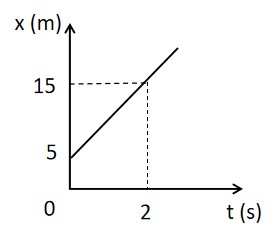
\includegraphics[scale=0.9]{../figs/VN11-Y21-PH-SYL-001-1.jpg}
		\end{center}
		\begin{mcq}(4)
			\item $x=5+5t$.
			\item $x=4t$.
			\item $x=5-5t$.
			\item $x=5+4t$.
		\end{mcq}
	}
	\loigiai
	{\textbf{Đáp án: A.}
		
		Vận tốc của vật là
		\begin{equation*}
			v=\dfrac{x-x_0}{t-t_0}=\dfrac{\SI{15}{\meter}-\SI{5}{\meter}}{\SI{2}{\second}}=\SI{5}{\meter/\second}.
		\end{equation*}
		
		Phương trình chuyển động của vật là
		\begin{equation*}
			x=x_0+vt=5+5t\textrm{ (m, s)}.
		\end{equation*}
		
		
	}
	\item \mkstar{3}
	
	\cauhoi{Khi ô tô đang chạy với vận tốc $\SI{10}{\meter/\second}$ trên đoạn đường thẳng thì người lái xe tăng ga và ô tô chuyển động nhanh dần đều. Sau $\SI{20}{\second}$, ô tô đạt vận tốc $\SI{14}{\meter/\second}$. Gia tốc $a$ và vận tốc $v$ của ô tô sau $\SI{40}{\second}$ kể từ lúc bắt đầu tăng ga là bao nhiêu?
		\begin{mcq}(2)
			\item $a=\SI{0.2}{\meter/\second}^2$; $v=\SI{18}{\meter/\second}$.
			\item $a=\SI{0.2}{\meter/\second}^2$; $v=\SI{8}{\meter/\second}$.
			\item $a=\SI{0.7}{\meter/\second}^2$; $v=\SI{38}{\meter/\second}$.
			\item $a=\SI{1.4}{\meter/\second}^2$; $v=\SI{66}{\meter/\second}$.
		\end{mcq}
	}
	\loigiai
	{\textbf{Đáp án: A.}
		
		Gia tốc của ô tô:
		$$a=\dfrac{v-v_0}{t}=\dfrac{\SI{14}{\meter/\second}-\SI{10}{\meter/\second}}{\SI{20}{\second}}=\SI{0.2}{\meter/\second^2}.$$
		Vận tốc của ô tô:
		$$v=v_0+at=\SI{10}{\meter/\second}+\SI{0.2}{\meter/\second^2}\cdot\SI{40}{\second}=\SI{18}{\meter/\second}.$$
		
		
	}
	\item \mkstar{3}
	
	\cauhoi{ Một vật chuyển động thẳng chậm dần đều với tốc độ ban đầu $\SI{4}{\meter/\second}$ và gia tốc có độ lớn $\SI{2}{\meter/\second^2}$. Biết thời điểm ban đầu vật ở gốc tọa độ và chuyển động cùng chiều dương của trục tọa độ. Phương trình chuyển động của vật là
		\begin{mcq}(2)
			\item $x=-4t-t^2$ (m, s).
			\item $x=4t-t^2$ (m, s).
			\item $x=4t-t^2$ (m, s).
			\item $x=-4t+t^2$ (m, s).
		\end{mcq}
	}
	\loigiai
	{\textbf{Đáp án: B.}
		
		Chọn gốc thời gian là khi vật bắt đầu chuyển động.
		
		Vì vật chuyển động chậm dần đều cùng chiều dương nên:
		\begin{equation*}
			\left\{\begin{array}{ll}{a\cdot v <0}&\\{v > 0}&\end{array}\right.\Rightarrow \left\{\begin{array}{ll}{a < 0}&\\{v > 0.}&\end{array}\right.
		\end{equation*}
		
		Kết hợp với các dữ kiện của đề bài, ta suy ra:
		\begin{equation*}
			\left\{\begin{array}{ll}{a=\SI{-2}{\meter/\second^2}}&\\{v=\SI{4}{\meter/\second} .}&\end{array}\right.
		\end{equation*}
		
		Phương trình chuyển động của vật có dạng:
		$x=4t-t^2$ (m, s).
		
		
	}
	\item \mkstar{3}
	
	\cauhoi{Một vật bắt đầu chuyển động từ trạng thái nghỉ với gia tốc không đổi $\SI{5}{\meter / \second \squared}$ trong $\SI{8}{\second}$. Sau thời gian này, vật chuyển động đều. Quãng đường vật đã đi được trong $\SI{12}{\second}$ kể từ lúc vật bắt đầu chuyển động là
		\begin{mcq}(4)
			\item $\SI{160}{\meter}$.
			\item $\SI{320}{\meter}$.
			\item $\SI{360}{\meter}$.
			\item $\SI{40}{\meter}$.
		\end{mcq}
	}
	\loigiai
	{\textbf{Đáp án: B.}
		
		Quãng đường vật đi được trong $\SI{8}{\second}$ đầu: $s_1=\dfrac{1}{2}at^2=\SI{160}{\meter}$.
		
		Vận tốc của vật ở cuối giây thứ 8: $v=at=\SI{40}{\meter / \second}$.
		
		Quãng đường vật đi được trong $\SI{4}{\second}$ sau:
		$s_2=vt=\SI{160}{\meter}$.
		
		Tổng quãng đường vật đã đi được trong $\SI{12}{\second}$ kể từ lúc vật bắt đầu chuyển động: $$s=s_1+s_2=\SI{320}{\meter}.$$
		
	}
	\item \mkstar{3}
	
	\cauhoi{Một ô tô đi từ A đến B. Đầu chặng ô tô đi 1/4 tổng thời gian với $v_1=\SI{50}{\km/\hour}$. Giữa chặng ô tô đi 1/2 tổng thời gian với $v_2=\SI{40}{\km/\hour}$. Cuối chặng ô tô đi 1/4 tổng thời gian với $v_3=\SI{20}{\km/\hour}$. Tốc độ trung bình của ô tô là
		\begin{mcq}(4)
			\item $\SI{37,5}{\kilo\meter/\hour}$.
			\item $\SI{50,2}{\kilo\meter/\hour}$.
			\item $\SI{70}{\kilo\meter/\hour}$.
			\item $\SI{85}{\kilo\meter/\hour}$.
		\end{mcq}
	}
	\loigiai
	{	\textbf{Đáp án: A.}
		
		Quãng đường ô tô đi đầu chặng là
		$$s_1=v_1t_1=v_1\cdot\dfrac{t}{4}.$$
		Quãng đường ô tô đi giữa chặng là
		$$s_2=v_2t_2=v_2\cdot\dfrac{t}{2}.$$
		Quãng đường ô tô đi cuối chặng là
		$$s_3=v_3t_3=v_3\cdot\dfrac{t}{4}.$$
		Tốc độ trung bình của ô tô là
		$$v_{\text{tb}}=\dfrac{s_1+s_2+s_3}{t}=\dfrac{v_1\cdot\dfrac{t}{4}+v_2\cdot\dfrac{t}{2}+v_3\cdot\dfrac{t}{4}}{t}=\dfrac{v_1}{4}+\dfrac{v_2}{2}+\dfrac{v_3}{4}=\SI{37,5}{\km/\hour}.$$
		
	
	}
	\item \mkstar{4}
	
	\cauhoi{Một người đang đi xe máy với vận tốc $\SI{36}{\kilo\meter/\hour}$ thì nhìn thấy chướng ngại vật cách đó $\SI{10}{\meter}$. Biết khối lượng tổng cộng của người và xe máy là $\SI{130}{\kilogram}$. Coi chuyển động của xe là chuyển động thẳng biến đổi đều sau khi hãm. Để không đâm phải chướng ngại vật thì vật phải có gia tốc nhỏ nhất là bao nhiêu?
		\begin{mcq}(4)
			\item $\SI{-5}{\meter/\second^2}$.
			\item $\SI{5}{\meter/\second^2}$.
			\item $\SI{-10}{\meter/\second^2}$.
			\item $\SI{10}{\meter/\second^2}$.
		\end{mcq}
		
	}
	\loigiai
	{\textbf{Đáp án: A.}
		
		Gia tốc nhỏ nhất để xe máy kịp dừng lại trước chướng ngại vật là:
		$$v^2-v_0^2=2a_\text{min} s\Rightarrow 0^2-(\SI{10}{\meter/\second})^2=2\cdot a_\text{min} \cdot \SI{10}{\meter}\Rightarrow a_\text{min}=\SI{-5}{\meter/\second^2}.$$
		
		
	}
	\item \mkstar{4}
	
	\cauhoi{ Một ôtô chạy đều trên một con đường thẳng với tốc độ $\SI{25}{\meter/\second}$ (vượt quá tốc độ) thì bị cảnh sát giao thông phát hiện. Chỉ sau $\SI{2}{\second}$ khi ôtô đi qua một cảnh sát, anh cảnh sát này bắt đầu đuổi theo với gia tốc không đổi và bằng $\SI{6}{\meter/\second^2}$. Thời điểm và vị trí anh cảnh sát đuổi kịp ôtô là
		\begin{mcq}
			\item sau $\SI{1}{\second}$ kể từ lúc anh cảnh sát xuất phát, cách vị trí xuất phát của anh cảnh sát $\SI{75}{\meter}$.
			\item  sau $\SI{10}{\second}$ kể từ lúc anh cảnh sát xuất phát, cách vị trí xuất phát của anh cảnh sát $\SI{300}{\meter}$.
			\item sau $\SI{12}{\second}$ kể từ lúc anh cảnh sát xuất phát, cách vị trí xuất phát của anh cảnh sát $\SI{300}{\meter}$.
			\item sau $\SI{3}{\second}$ kể từ lúc anh cảnh sát xuất phát, cách vị trí xuất phát của anh cảnh sát $\SI{75}{\meter}$.
		\end{mcq}
	}
	\loigiai
	{\textbf{Đáp án: B.}
		
		Chọn chiều dương là chiều chuyển động của xe ôtô và anh cảnh sát, gốc tọa tọa là vị trí của anh cảnh sát đang đứng, gốc thời gian là thời điểm cảnh sát bắt đầu đuổi theo xe.
		
		Phương trình chuyển động của xe ôtô là
		$$x=x_0+v_0(t+2)=25(t+2)\ \text{(m; s)}.$$
		
		Phương trình chuyển động của anh cảnh sát là
		$$x'=x_0'+v_0't+\dfrac{1}{2}at^2=3t^2\ \text{(m; s)}.$$
		
		Thời điểm anh cảnh sát đuổi kịp xe ôtô là
		$$x=x'\Rightarrow 25(t+2)=3t^2\Rightarrow t=\SI{10}{\second}.$$
		
		Vị trí anh cảnh sát đuổi kịp xe ôtô là
		$$x'=3t^2=\SI{300}{\meter}.$$
		
		
	}
	\item \mkstar{4}
	
	\cauhoi{Hai chất điểm A và B cách nhau $\SI{60}{\meter}$. Tại thời điểm $t=0$ chất điểm A chuyển động về phía B với vận tốc không đổi $\SI{12}{\meter / \second}$. Cùng thời điểm đó chất điểm B cũng chuyển động với gia tốc $\SI{2}{\meter / \second \squared}$ theo hướng ra xa A. Khoảng cách giữa A và B ngắn nhất tại thời điểm
		\begin{mcq}(4)
			\item $t=\SI{4}{\second}$.
			\item $t=\SI{5}{\second}$.
			\item $t=\SI{6}{\second}$.
			\item $t=\SI{2}{\second}$.
		\end{mcq}
	}
	\loigiai
	{\textbf{Đáp án: C.}
		
		Chọn chiều dương của trục $\text O x$ cùng hướng chuyển động của A và B, gốc O tại vị trí ban đầu của A. Gốc thời gian là lúc vật A và B bắt đầu chuyển động.
		
		Phương trình chuyển động của A: $x_\text A = 12t$.
		
		Phương trình chuyển động của B: $x_\text B = t^2 + 60$.
		
		Khoảng cách giữa A và B: $|x_\text B - x_\text A |=|t^2+60-12t|=|(t-6)^2+24|$.
		
		Khoảng cách này nhỏ nhất khi $(t-6)^2 = 0 \Rightarrow t=\SI{6}{\second}$.
		
		
	}
\end{enumerate}

\whiteBGstarEnd

\loigiai{\begin{center}
		\textbf{BẢNG ĐÁP ÁN}
	\end{center}
	\begin{center}
		\begin{tabular}{|m{2.8em}|m{2.8em}|m{2.8em}|m{2.8em}|m{2.8em}|m{2.8em}|m{2.8em}|m{2.8em}|m{2.8em}|m{2.8em}|}
			\hline
			1.C  & 2.A  & 3.B  & 4.B  & 5.C  & 6.A  & 7.C  & 8.C  & 9.D  & 10.D  \\
			\hline
			11.C  & 12.A  & 13.A  & 14.A  & 15.B  & 16.B  & 17.A  & 18.A  & 19.B  & 20.C  \\
			\hline
			
		\end{tabular}
\end{center}}
\chapter{Pre-course: Sự rơi tự do - Chuyển động tròn đều}
\whiteBGstarBegin

\begin{enumerate}[label=\bfseries Câu \arabic*:]
	
	\item \mkstar{1}
	
	\cauhoi
	{Câu nào sau đây là đúng khi nói về sự rơi?
		\begin{mcq}
			\item Khi không có sức cản vật nặng rơi nhanh hơn vật nhẹ.
			\item Ở cùng một nơi, mọi vật rơi tự do có cùng gia tốc.
			\item Khi rơi tự do, vật nào ở độ cao lớn hơn sẽ rơi với gia tốc lớn hơn.
			\item Vận tốc của vật chạm đất không phụ thuộc vào độ cao của vật khi rơi.
		\end{mcq}
	}
	
	\loigiai
	{\textbf{Đáp án: B.}
		
		Gia tốc rơi tự do không phụ thuộc vào khối lượng của vật, chỉ phụ thuộc vào vĩ độ địa lý, độ cao và cấu trúc địa chất nơi đó nên ở cùng một nơi, mọi vật rơi tự do có cùng gia tốc.
		
		
	}
	\item \mkstar{1}
	
	\cauhoi
	{Chuyển động của vật nào dưới đây được coi là chuyển động tròn đều?
		\begin{mcq}
			\item Chuyển động của bánh xe ôtô khi đang hãm phanh.
			\item Chuyển động quay của cánh quạt khi quay ổn định.
			\item Chuyển động quay của các điểm treo các ghế ngồi trên chiếc đu quay.
			\item Chuyển động quay của cánh quạt khi vừa tắt điện.
		\end{mcq}
		
	}
	\loigiai
	{\textbf{Đáp án: B.}
		
		Chuyển động quay của cánh quạt khi quay ổn định là chuyển động tròn đều.
		
	}
	\item \mkstar{1}
	
	\cauhoi
	{Các công thức liên hệ giữa tốc độ góc $\omega$ với chu kỳ $T$ và giữa tốc độ góc $\omega$ với tần số $f$ trong chuyển động tròn đều là gì?
		\begin{mcq}(2)
			\item $\omega=2\pi T$; $\omega=\dfrac{2\pi}{f}$.
			\item $\omega=\dfrac{2\pi}{T}$; $\omega=2\pi f$.
			\item $\omega=2\pi T$; $\omega=2\pi f$. 
			\item $\omega=\dfrac{2\pi}{T}$; $\omega=\dfrac{2\pi}{f}$.
		\end{mcq}
		
	}
	\loigiai
	{\textbf{Đáp án: B.}
		
		Công thức liên hệ giữa tốc độ góc $\omega$ với chu kỳ $T$ là $\omega=\dfrac{2\pi}{T}$.
		Công thức liên hệ giữa giữa tốc độ góc $\omega$ với tần số $f$ trong chuyển động tròn đều là $\omega=2\pi f$.
	
	}
	
	\item \mkstar{2}
	
	\cauhoi
	{Người ta thả một vật rơi tự do, sau $\SI{5}{\second}$ vật chạm đất, $g=\SI{9.8}{\meter/\second^2}$. Độ cao thả vật là
		\begin{mcq}(4)
			\item $\SI{122.5}{\meter}$.
			\item $\SI{61.25}{\meter}$.
			\item $\SI{254}{\meter}$.
			\item $\SI{183,75}{\meter}$.
		\end{mcq}
	}
	\loigiai
	{\textbf{Đáp án: A.}	
		
		Độ cao lúc thả vật là
		$h=s=\dfrac{1}{2}gt^2=\dfrac{1}{2}\cdot\SI{9.8}{\meter/\second^2}\cdot(\SI{5}{\second})^2=\SI{122.5}{\meter}.$
		
		
	}
	\item \mkstar{2}
	
	\cauhoi
	{Cùng một lúc tại mái nhà, bi A được thả rơi còn bi B được ném theo phương ngang. Bi A có khối lượng gấp đôi bi B. Bỏ qua sức cản của không khí thì
		\begin{mcq}
			\item bi A chạm đất trước bi B.
			\item bi B chạm đất trước bi A.
			\item cả hai chạm đất cùng lúc.
			\item chưa đủ điều kiện để kết luận bi A hay bi B chạm đất trước.
		\end{mcq}
		
	}
	\loigiai
	{\textbf{Đáp án: C.}
		
		Sự rơi tự do nhanh hay chậm không phụ thuộc vào khối lượng $\left( t=\sqrt{\dfrac{2h}{g}}\right)$.
		
		Do đó hai bi chạm đất cùng lúc.
		
		
	}
	
	\item \mkstar{2}
	
	\cauhoi
	{Một bánh xe có đường kính $\SI{100}{\centi\meter}$ lăn đều với vận tốc $\SI{36}{\kilo\meter/\hour}$. Gia tốc hướng tâm của một điểm trên vành bánh xe có độ lớn
		\begin{mcq}(4)
			\item $\SI{200}{\meter/\second^2}$.
			\item $\SI{400}{\meter/\second^2}$.
			\item $\SI{100}{\meter/\second^2}$.
			\item $\SI{300}{\meter/\second^2}$.
		\end{mcq}
	}
	\loigiai
	{\textbf{Đáp án: A.}
		
		Đổi đơn vị: $\SI{100}{\centi\meter}=\SI{1}{\meter}$; $\SI{36}{\kilo\meter/\hour}=\SI{10}{\meter/\second}$
		
		Gia tốc hướng tâm của một điểm trên vành bánh xe có độ lớn:
		$$a_\text{ht}=\dfrac{v^2}{R}=\SI{200}{\meter/\second^2}.$$
		
		
	}
	\item \mkstar{2}
	
	\cauhoi
	{Thả hai vật rơi tự do đồng thời từ hai độ cao $h_1$ và $h_2$. Biết rằng thời gian chạm đất của vật thứ nhất bằng 2 lần của vật thứ hai. Tỉ số $\dfrac{h_1}{h_2}$ là
		\begin{mcq}(4)
			\item $\dfrac{h_1}{h_2}=4$.
			\item $\dfrac{h_1}{h_2}=\dfrac{1}{2}$.
			\item $\dfrac{h_1}{h_2}=2$.
			\item $\dfrac{h_1}{h_2}=\dfrac{1}{4}$.
		\end{mcq}
	}
	\loigiai
	{\textbf{Đáp án: A.}
		
		Tỉ số $\dfrac{h_1}{h_2}$ có thể được suy ra từ việc lập tỉ số độ cao của hai vật: $$\dfrac{h_1}{h_2}=\dfrac{\dfrac{1}{2}gt_1^2}{\dfrac{1}{2}gt_2^2}=\dfrac{t_1^2}{t_2^2}=\left( \dfrac{t_1}{t_2}\right)^2=4.$$
		
		
	}
	\item \mkstar{2}
	
	\cauhoi
	{Một đĩa tròn bán kính $\SI{20}{\centi\meter}$ quay đều quanh trục của nó. Đĩa quay hết 1 vòng mất $\SI{0.2}{\second}$. Tốc độ dài $v$ của một điểm nằm ở mép đĩa bằng
		\begin{mcq}(4)
			\item $\SI{4,71}{\meter/\second}$. 
			\item $\SI{3,14}{\meter/\second}$. 
			\item $\SI{6,28}{\meter/\second}$. 
			\item $\SI{7,85}{\meter/\second}$. .
		\end{mcq}
		
	}
	\loigiai
	{\textbf{Đáp án: C.}
		
		Tốc độ dài $v$ của một điểm trên vành ngoài xe:
		$v=r\omega=r\dfrac{\Delta \alpha}{\Delta t}=\SI{0,2}{\meter}\dfrac{2\pi}{\SI{0.2}{\second}}=\SI{6,28}{\meter/\second}$
		
		
	}
	\item \mkstar{2}
	
	\cauhoi
	{Một động cơ xe máy có trục quay 1200 vòng/ phút. Tốc độ góc của chuyển động quay là bao nhiêu?
		\begin{mcq}(4)
			\item $\SI{125,7}{\radian/\second}$.
			\item $\SI{188,5}{\radian/\second}$.
			\item $\SI{62,8}{\radian/\second}$.
			\item $\SI{7200}{\radian/\second}$.
		\end{mcq}
	}
	\loigiai
	{\textbf{Đáp án: A.}
		
		Tốc độ góc của chuyển động quay là:
		$\omega$ = 1200 vòng/ phút = $1200\cdot\dfrac{2\pi}{60}\,\SI{}{\radian/\second}=\SI{125,7}{\radian/\second}$
		
		
	}
	\item \mkstar{2}
	
	\cauhoi
	{Một bánh xe có bán kính $\SI{100}{\centi\meter}$ lăn đều với vận tốc $\SI{54}{\kilo\meter/\hour}$. Gia tốc hướng tâm của một điểm trên vành bánh xe có độ lớn
		\begin{mcq}(4)
			\item $\SI{225}{\meter/\second^2}$.
			\item $\SI{400}{\meter/\second^2}$.
			\item $\SI{100}{\meter/\second^2}$.
			\item $\SI{300}{\meter/\second^2}$.
		\end{mcq}
	}
	\loigiai
	{\textbf{Đáp án: A.}
		
		Gia tốc hướng tâm của một điểm trên vành bánh xe có độ lớn:
		$$a_\text{ht}=\dfrac{v^2}{R}=\SI{225}{\meter/\second^2}.$$
		
		
	}
	\item \mkstar{2}
	
	\cauhoi
	{Một hòn đá thả rơi tự do từ đỉnh toà nhà $25$ tầng nó chạm đất trong thời gian $5\ \text{s}$. Lấy $g=10\ \text{m/s}^2$. Trong giây đầu tiên hòn đá đã đi qua số tầng của toà nhà là
		\begin{mcq}(4)
			\item $1$.
			\item $2$.
			\item $3$.
			\item $5$.
		\end{mcq}
	}
	\loigiai
	{\textbf{Đáp án: A.}
		
		Gọi chiều cao mỗi tầng nhà là $h$. 
		
		Suy ra $25h=g\dfrac{5^2}{2}\Rightarrow h=5\ \text{m}$.
		
		Gọi $n$ là số tầng trong giây đầu hòn đá rơi được.
		
		Suy ra $n\cdot 5=g\cdot \dfrac{1^2}{g}\Rightarrow n=1$.
		
		
	}
	\item \mkstar{3}
	
	\cauhoi
	{Từ đỉnh tháp hai vật A và B được thả rơi tự do. Biết B được thả rơi sau A $1\ \text{s}$. Lấy $g=10\ \text{m/s}^2$. Khoảng cách giữa A và B tại thời điểm sau khi B rơi được $2\ \text{s}$ là
		\begin{mcq}(4)
			\item $5\ \text{m}$.
			\item $10\ \text{m}$.
			\item $20\ \text{m}$.
			\item $25\ \text{m}$.
		\end{mcq}
		
	}
	\loigiai
	{\textbf{Đáp án: D.}
		
		Tại thời điểm sau khi B rơi được $2\ \text{s}$, A đã rơi được $3\ \text{s}$
		
		Suy ra, khoảng cách giữa A và B là
		
		$$\Delta h=g\cdot\dfrac{t_1^2}{2}-g\cdot\dfrac{t_2^2}{2}=\dfrac{10}{2}\cdot \left( 3^2-2^2\right)=25\ \text{m}$$
		
		
		
	}
	\item \mkstar{3}
	
	\cauhoi
	{Một người thả vật rơi tự do, vật chạm đất có $v=\SI{36}{\meter/\second}$, $g=\SI{10}{\meter/\second^2}$. Độ cao của vật sau khi thả được $\SI{3}{\second}$ là
		\begin{mcq}(4)
			\item $\SI{64.8}{\meter}$
			\item $\SI{19.8}{\meter}$
			\item $\SI{86.4}{\meter}$
			\item $\SI{45.0}{\meter}$
		\end{mcq}
	}
	\loigiai
	{\textbf{Đáp án: B.}
		
		Độ cao nơi thả vật:
		$$v=\sqrt{2gh}\Rightarrow h = \SI{64.8}{\meter}.$$
		Quãng đường vật rơi $\SI{3}{\second}$ đầu tiên là
		$$s_3=\dfrac{1}{2}gt^2=\dfrac{1}{2}\cdot\SI{10}{\meter/\second^2}\cdot(\SI{3}{\second})^2=\SI{45}{\meter}.$$
		Độ cao của vật lúc này:
		$$h=s-s_3=\SI{64.8}{\meter}-\SI{45}{\meter}=\SI{19.8}{\meter}.$$
		
		
	}
	\item \mkstar{3}
	
	\cauhoi
	{Các giọt nước mưa đang rơi từ mái nhà xuống sau những khoảng thời gian bằng nhau. Khi giọt thứ nhất chạm đất thì giọt thứ năm bắt đầu rơi, lúc đó khoảng cách giữa giọt thứ nhất và giọt thứ hai là $\SI{14}{\meter}$. Lấy $g=\SI{10}{\meter/\second^2}$. Độ cao mái nhà là
		\begin{mcq}(4)
			\item $\SI{32}{\meter}$.
			\item $\SI{9}{\meter}$.
			\item $\SI{56}{\meter}$.
			\item $\SI{16}{\meter}$.
		\end{mcq}
	}
	\loigiai
	{\textbf{Đáp án: A.}
		
		Gọi $\Delta t$ khoảng thời gian bằng nhau các giọt nước mưa đang rơi từ mái nhà xuống.
		
		Quãng đường giọt thứ nhất rơi cho đến khi chạm đất là
		$$s_1=\dfrac{1}{2}g(4\Delta t)^2.$$
		Quãng đường giọt thứ hai rơi cho đến khi giọt thứ nhất chạm đất là
		$$s_2=\dfrac{1}{2}g(3\Delta t)^2.$$
		Theo đề bài ta có:
		$$\Delta s= s_1-s_2=\dfrac{7}{2}g(\Delta t)^2=\SI{14}{\meter}\Rightarrow \Delta t=\dfrac{\sqrt{10}}{5}\,\text{s}.$$
		Độ cao mái nhà là
		$$h=s_1=\dfrac{1}{2}g(4\Delta t)^2=\SI{32}{\meter}.$$
		
		
	}
	\item \mkstar{3}
	
	\cauhoi
	{Một vệ tinh nhân tạo ở độ cao $\SI{250}{\kilo\meter}$ bay quanh Trái Đất theo một quỹ đạo tròn. Chu kì của vệ tinh là 88 phút. Tính tốc độ góc và gia tốc hướng tâm của vệ tinh. Cho bán kính Trái Đất là $\SI{6400}{\kilo\meter}$.
		\begin{mcq}(4)
			\item $\SI{9,41}{ \meter/\second^2}$.
			\item $\SI{9,48}{ \meter/\second^2}$.
			\item $\SI{8,72}{ \meter/\second^2}$.
			\item $\SI{10,05}{ \meter/\second^2}$.
		\end{mcq}
	}
	\loigiai
	{	\textbf{Đáp án: A.}
		
		Khoảng cách từ vệ tinh đến tâm Trái Đất: 
		$$r=\SI{250}{\kilo\meter}+\SI{6400}{\kilo\meter} =\SI{6650}{\kilo\meter}=\SI{6650000}{\meter}.$$
		
		Tốc độ góc của vệ tinh:
		$$T=\frac{2\pi}{\omega} \Rightarrow \omega = \frac{\pi}{2640}\ \text{rad/s}.$$ 
		
		Gia tốc hướng tâm của vệ tinh: 
		
		$$a_{ht}=\omega^2 \cdot r \approx \SI{9,41}{ \meter/\second^2}.$$
		
		
	
	}
	\item \mkstar{3}
	
	\cauhoi
	{Một hòn đá rơi tự do từ cửa sổ một toà nhà cao tầng. Sau đó $1\ \text{s}$ tại ban công phía dưới cách cửa sổ trên của toà nhà $20\ \text{m}$ có một hòn đá khác cũng rơi tự do. Biết cả hai hòn đá cùng chạm đất đồng thời. Lấy $g=10\ \text{m/s}^2$. Chiều cao của cửa sổ toà nhà trên so với đất là	
		\begin{mcq}(4)
			\item $\text{25,31}\ \text{m}$.
			\item $\text{31,25}\ \text{m}$.
			\item $\text{51,25}\ \text{m}$.
			\item $\text{35,31}\ \text{m}$.
		\end{mcq}
	}
	\loigiai
	{\textbf{Đáp án: B.}	
		
		Ta có: $h=g\cdot \dfrac{t^2}{2}; \ h-20=g\cdot \dfrac{\left(t-1 \right)^2 }{2}$.
		
		$\Rightarrow t=\text{2,5}\ \text{s}; \ h=\text{31,25}\ \text{m}$.  
		
		
	}
	\item \mkstar{3}
	
	\cauhoi
	{Một vật rơi tự do từ độ cao $250\ \text{m}$. Tỉ số quãng đường vật rơi được trong $2\ \text{s}$ đầu, $2\ \text{s}$ sau và $2\ \text{s}$ cuối cùng là
		\begin{mcq}(4)
			\item $1:4:9$.
			\item $1:2:4$.
			\item $1:3:5$.
			\item $1:2:3$.
		\end{mcq}
	}
	\loigiai
	{\textbf{Đáp án: C.}
		
		Rơi tự do là chuyển động nhanh dần đều với $V_0=0$  nên khi thời gian chuyển động trên các đoạn đường liên tiếp bằng nhau (cùng bằng $2\ \text{s}$) thì: $\Delta s_1:\Delta s_2:\Delta s_3=1:3:5$.
		
		
	}
	\item \mkstar{4}
	
	\cauhoi
	{Một viên bi A được thả rơi từ độ cao $\SI{30}{\meter}$. Cùng lúc đó, một viên bi B được bắn theo phương thẳng đứng từ dưới đất lên với $\SI{25}{\meter/\second}$ tới va chạm vào bi A. Chọn trục O$y$ thẳng đứng, gốc O ở mặt đất, chiều dương hướng lên, gốc thời gian lúc 2 viên bi bắt đầu chuyển động, $g=\SI{10}{\meter/\second^2}$. Bỏ qua sức cản không khí. Thời điểm và tọa độ 2 viên bi gặp nhau là
		\begin{mcq}(2)
			\item $\SI{1.2}{\second}$ và $\SI{22.8}{\meter}$.
			\item $\SI{1.6}{\second}$ và $\SI{11.4}{\meter}$.
			\item $\SI{1.4}{\second}$ và $\SI{8.8}{\meter}$.
			\item $\SI{1.8}{\second}$ và $\SI{1.6}{\meter}$.
		\end{mcq}
	}
	\loigiai
	{\textbf{Đáp án: A.}
		
		Phương trình chuyển động của viên bi A là
		$$y_{\text{A}}=y_{0\text{A}}+v_{0\text{A}}t+\dfrac{1}{2}gt^2=30-5t^2 \textrm{ (m, s)}.$$
		Phương trình chuyển động của viên bi B là
		$$y_{\text{B}}=y_{0\text{B}}+v_{0\text{B}}t+\dfrac{1}{2}gt^2=25t-5t^2\textrm{ (m, s)}.$$
		Hai viên bi gặp nhau khi chúng có cùng tọa độ:
		$$y_{\text{A}}=y_{\text{B}}\Rightarrow 30-5t^2=25t-5t^2 \Rightarrow t=\SI{1.2}{\second}.$$
		Tọa độ hai viên bi khi gặp nhau là
		$$y_{\text{A}}=y_{\text{B}}=30-5t^2=\SI{22.8}{\meter}.$$
		
		
	}
	\item \mkstar{4}
	
	\cauhoi
	{Hai viên bi sắt được thả rơi cùng độ cao cách nhau một khoảng thời gian $\SI{0,5}{\second}$. Lấy $g = \SI{10}{\meter/\second^2}$. Khoảng cách giữa hai viên bi sau khi viên thứ nhất rơi được $\SI{1,5}{\second}$ là
		\begin{mcq}(4)
			\item $\SI{12,5}{\meter}$.
			\item $\SI{6,25}{\meter}$.
			\item $\SI{5,0}{\meter}$.
			\item $\SI{2,5}{\meter}$.
		\end{mcq}
	}
	\loigiai
	{\textbf{Đáp án: B.}
		
		Chọn gốc thời gian là lúc thả viên bi 1. Viên bi 2 được thả sau $\SI{0,5}{\second}$ nên:
		$$t_2=t_1-\SI{0,5}{\second}$$
		Quãng đường viên bi 1 đi được:
		$$s_1=\frac{1}{2}gt_1^2.$$
		Quãng đường viên bi 2 đi được:
		$$s_2=\frac{1}{2}g(t_1-0,5)^2$$
		Lấy $s_1-s_2=\dfrac{1}{2}gt_1^2-\dfrac{1}{2}g(t_1-0,5)^2=\SI{6,25}{\meter}$.
		
		
	}
	\item \mkstar{4}
	
	\cauhoi
	{Quãng đường vật rơi trong giây thứ $n$ là $h$. Quãng đường mà nó rơi trong giây tiếp theo là
		\begin{mcq}(4)
			\item $h$.
			\item $h+\dfrac{g}{2}$.
			\item $h-g$.
			\item $h+g$.
		\end{mcq}
		
		
	}
	\loigiai
	{\textbf{Đáp án: D.}
		
		Quãng đường vật rơi được trong giây thứ $n$ bằng quãng đường vật rơi được từ ban đầu cho đến giây $n$ trừ cho quãng đường vật rơi được từ ban đầu cho đến giây $n-1$: $$h=\dfrac{1}{2}gn^2-\dfrac{1}{2}g(n-1)^2=\dfrac{g}{2}(2n-1)$$
		
		Quãng đường vật rơi được trong giây thứ $n+1$ bằng quãng đường vật rơi được từ ban đầu cho đến giây $n+1$ trừ cho quãng đường vật rơi được từ ban đầu cho đến giây $n$:
		$$h'=\dfrac{1}{2}g(n+1)^2-\dfrac{1}{2}gn^2 = \dfrac{g}{2}(2n+1)$$
		
		Vậy $h'=h+g$.
		
		
	}
\end{enumerate}

\whiteBGstarEnd

\loigiai{\begin{center}
		\textbf{BẢNG ĐÁP ÁN}
	\end{center}
	\begin{center}
		\begin{tabular}{|m{2.8em}|m{2.8em}|m{2.8em}|m{2.8em}|m{2.8em}|m{2.8em}|m{2.8em}|m{2.8em}|m{2.8em}|m{2.8em}|}
			\hline
			1. B  & 2.B  & 3.B  & 4.A  & 5.C  & 6.A  & 7.A  & 8.C  & 9.A  & 10.A  \\
			\hline
			11.A  & 12.D  & 13.B  & 14.A  & 15.A  & 16.B  & 17.C  & 18.A  & 19.B  & 20.D  \\
			\hline
			
		\end{tabular}
\end{center}}
\chapter{Pre-course: Tổng hợp và phân tích lực. Điều kiện cân bằng của chất điểm}
\whiteBGstarBegin

\begin{enumerate}[label=\bfseries Câu \arabic*:]
	
	\item \mkstar{1}
	
	\cauhoi{ Muốn cho một chất điểm cân bằng thì hợp lực của các lực tác dụng lên nó phải	
		\begin{mcq}(2)
			\item không đổi.
			\item thay đổi.
			\item bằng không.
			\item khác không.
		\end{mcq}
	}
	
	\loigiai{\textbf{Đáp án: C.}
		
		Muốn cho một chất điểm cân bằng thì hợp lực của các lực tác dụng lên nó phải bằng 0.
		
		
	}
	\item \mkstar{1}
	
	\cauhoi{ Độ lớn của hợp lực $\vec{F}$ hai lực $\vec{F}_1$ và $\vec{F}_2$  đồng qui hợp với nhau góc $\alpha$ là
		\begin{mcq}(2)
			\item $\sqrt{F_1^2+F_2^2-2F_1F_2\cos \alpha}$.
			\item $\sqrt{F_1^2+F_2^2+2F_1F_2\cos \alpha}$.
			\item $\sqrt{F_1^2+F_2^2-F_1F_2\cos \alpha}$.
			\item $\sqrt{F_1^2+F_2^2+F_1F_2\cos \alpha}$.
		\end{mcq}
	}
	\loigiai{\textbf{Đáp án: B.}
		
		Ta có: $$F = \sqrt{F_1^2+F_2^2+2F_1F_2\cos \alpha}.$$
		
		
	}
	\item \mkstar{1}
	
	\cauhoi{ Tổng hợp lực là 
		\begin{mcq}
			\item thay thế một lực bằng các lực có tác dụng giống hệt như các lực ấy.
			\item thay thế các lực tác dụng đồng thời vào cùng một vật bằng một lực có tác dụng giống hệt như các lực ấy.
			\item thay thế các lực tác dụng đồng thời hai vật bằng một lực có tác dụng giống hệt như các lực ấy.
			\item thay thế hai lực bằng ba lực có tác dụng giống hệt như các lực ấy.
		\end{mcq}
	}
	\loigiai{\textbf{Đáp án: B.}
		
		Tổng hợp lực là thay thế các lực tác dụng đồng thời vào cùng một vật bằng một lực có tác dụng giống hệt như các lực ấy.
		
		
	}
	\item \mkstar{2}
	
	\cauhoi{ Một chất điểm đứng yên dưới tác dụng của $3$ lực có độ lớn bằng nhau. Kết luận nào sau đây là đúng?
		\begin{mcq}
			\item 	Có 2 lực cùng giá, ngược chiều nhau.
			\item  Ba lực có giá cùng nằm trong 1 mặt phẳng, chúng lần lượt hợp với nhau những góc $120^\circ$.
			\item Ba lực có giá cùng nằm trong một mặt phẳng, trong đó $2$ lực có giá vuông góc nhau.
			\item A, B, C đều sai.
			
		\end{mcq}
	}
	\loigiai{\textbf{Đáp án: B.}	
		
		Một chất điểm đứng yên dưới tác dụng của $3$ lực có độ lớn bằng nhau thì ba lực có giá cùng nằm trong 1 mặt phẳng, chúng lần lượt hợp với nhau những góc $120^\circ$.
		
		
	}
	\item \mkstar{2}
	
	\cauhoi{ Tác dụng vào một vật đồng thời hai lực $\vec{F_1}$  và $\vec{F_2}$ trong đó độ lớn $F_1 = 30\ \text{N}$ và $F_1 = 40\ \text{N}$. Nhận xét nào sau đây là đúng?
		\begin{mcq}
			\item Hợp lực tác dụng lên vật có độ lớn $70\ \text{N}$.
			\item Hợp lực tác dụng lên vật có độ lớn $10\ \text{N}$.
			\item Hợp lực tác dụng lên vật có độ lớn $50\ \text{N}$.
			\item Chưa đủ cơ sở để kết luận.
		\end{mcq}
	}
	\loigiai{\textbf{Đáp án: D.}
		
		Vì chưa biết $\alpha$ hợp bởi hai lực  $\vec{F_1}$  và $\vec{F_2}$ nên ta chưa đủ cơ sở để kết luận.
		
		
	}
	\item \mkstar{2}
	
	\cauhoi{ Hai lực $\vec{F_1}$  và $\vec{F_2}$ có cùng độ lớn  hợp với nhau một góc $\alpha$. Hợp lực của chúng có độ lớn là
		\begin{mcq}(2)
			\item $F=F_1+F_2$.
			\item $F=|F_1-F_2|$.
			\item $F=2F_1\cos \alpha$.
			\item $F=2F_1\cos \left( \dfrac{\alpha}{2}\right) $.
		\end{mcq}
	}
	\loigiai{\textbf{Đáp án: D.}
		
		Hai lực $\vec{F_1}$  và $\vec{F_2}$ có cùng độ lớn  hợp với nhau một góc $\alpha$. Hợp lực của chúng có độ lớn là  $F=2F_1\cos \left( \dfrac{\alpha}{2}\right) $.
		
		
	}
	\item \mkstar{2}
	
	\cauhoi{Chọn câu trả lời đúng. Cho hai lực đồng qui có độ lớn là $70\ \text{N}$ và $120\ \text{N}$. Hợp lực của hai lực có thể là
		\begin{mcq}(4)
			\item $40\ \text{N}$.
			\item $69\ \text{N}$.
			\item $192\ \text{N}$.
			\item $200\ \text{N}$.
		\end{mcq}
	}
	\loigiai{\textbf{Đáp án: B.}
		
		$|F_1-F_2|\leq F\leq F_1+F_2$ hay $50\ \text{N}\leq F\leq 190\ \text{N}$. 
		
		Vậy ta chọn giá trị $F=69\ \text{N}$.
		
		
	}
	\item \mkstar{2}
	
	\cauhoi{ Điều nào sau đây là \textbf{sai} khi nói về đặc điểm của hai lực cân bằng? 
		
		\begin{mcq}(2)
			\item Hai lực có cùng giá.
			\item Hai lực đặt vào hai vật khác nhau.
			\item Hai lực ngược chiều nhau.
			\item Hai lực có cùng độ lớn.
		\end{mcq}
	}
	\loigiai{\textbf{Đáp án: B.}
		
		Hai lực cân bằng đặt vào cùng một vật.
	
	}
	\item \mkstar{2}
	
	\cauhoi{Chọn câu trả lời đúng. Cho hai lực đồng quy có độ lớn bằng $150\ \text{N}$ và $200\ \text{N}$. Trong số các giá trị sau đây, giá trị nào là độ lớn của hợp lực?
		\begin{mcq}(4)
			\item $40\ \text{N}$.
			\item $250\ \text{N}$.
			\item $400\ \text{N}$.
			\item $500\ \text{N}$.
		\end{mcq}
	}
	\loigiai{\textbf{Đáp án: B.}
		
		$|F_1-F_2|\leq F\leq F_1+F_2$ hay $50\ \text{N}\leq F\leq 350\ \text{N}$. 
		
		Vậy ta chọn giá trị $F=250\ \text{N}$.
		
		
	}
	\item \mkstar{2}
	
	\cauhoi{ Một trái banh được tác dụng lực $\vec{F_1}$ bởi gió và $\vec{P}$ bởi trọng lực, hai lực này có giá vuông góc với nhau và độ lớn $F_1=P=\SI{10}{N}$. Hãy tính độ lớn của lực $\vec{F_3}$ là lực tổng hợp của hai lực trên.
		\begin{mcq}(4)
			\item $F_3= 10\sqrt{2}\, \textrm{N}$.
			\item $F_3= 10\sqrt{3}\, \textrm{N}$.
			\item $F_3= 10\, \textrm{N}$.
			\item $F_3= 20\, \textrm{N}$.
		\end{mcq}
		
	}
	\loigiai{\textbf{Đáp án: A.}
		
		Do hai vectơ vuông góc nhau nên $$F_3= \sqrt{F_1^2+P^2}=10\sqrt{2}\, \textrm{N}$$
		
		
	}
	\item \mkstar{2}
	
	\cauhoi{ Hai lực có giá đồng quy có độ lớn $F_1=F_2=10\ N$, có $(\overrightarrow {F_1}, \overrightarrow {F_2})=60^\circ$. Hợp lực của hai lực này có độ lớn là
		\begin{mcq}(4)
			\item $\text{17,3}\, \si{\newton}$.
			\item $\text{20}\, \si{\newton}$.
			\item $\text{14,1}\, \si{\newton}$.
			\item $\text{10}\, \si{\newton}$.
		\end{mcq}
		
	}
	\loigiai{\textbf{Đáp án: A.}
		
		Áp dụng công thức $$F^2=F_1^2+F_2^2+2F_1F_2.\cos(\overrightarrow {F_1}, \overrightarrow {F_2}) $$
		
		Thay số liệu vào, ta tìm được $$F=\text{17,3}\, \si{\newton}$$
		
		
	}
	\item \mkstar{3}
	
	\cauhoi{ Một chất điểm chịu tác dụng đồng thời của hai lực thành phần có độ lớn $F_1$ và $F_2$ thì hợp lực F của chúng luôn có độ lớn thỏa mãn hệ thức:
		\begin{mcq}(2)
			\item $F=F_1^2+F_2^2$.
			\item $F = F_1 + F_2$.
			\item $|F_1-F_2| \leq F \leq F_1 + F_2$.
			\item $F= \sqrt{F_1^2+F_2^2}$.
		\end{mcq}
		
	}
	\loigiai{\textbf{Đáp án: C.}
		
		Theo lý thuyết:	$$|F_1-F_2| \leq F \leq F_1 + F_2$$
		
		
	}
	\item \mkstar{3}
	
	\cauhoi{	Hai lực thành phần $\vec{F_1}$ và $\vec{F_2}$ có độ lớn là $F_1= \text{50}\, \si{\newton}$ và $F_2=\text{35}\, \si{\newton}$ đồng qui, hợp nhau một góc $180^\circ$ thì hợp lực $\vec{F}$ của chúng có độ lớn bằng	
		\begin{mcq}(4)
			\item $\text{15}\, \si{\newton}$.
			\item $\text{85}\, \si{\newton}$.
			\item $\text{7,5}\, \si{\newton}$.
			\item$\text{42,5}\, \si{\newton}$.
		\end{mcq}
		
	}
	\loigiai{\textbf{Đáp án: A.}
		
		Khi $\vec{F_1} \uparrow \downarrow \vec{F_2} $ thì $F_\text{min}=|F_1-F_2|=\text{15}\, \si{\newton}$.
		
		
	}
	\item \mkstar{3}
	
	\cauhoi{ Ba lực thành phần đồng phẳng, đồng qui $F_1, F_2, F_3$ có độ lớn bằng nhau và bằng 120N. Khi ba lực đó hợp nhau một góc $120^\circ$ từng đôi một thì hợp lực $\vec F$ của chúng có độ lớn bằng
		\begin{mcq}(4)
			\item 0 N.
			\item 120 N.
			\item 120 N.
			\item 360 N.
		\end{mcq}
		
	}
	\loigiai{\textbf{Đáp án: A.}
		
		Khi $$F_1=F_2$$ $$\Rightarrow F_{12}=2F_1 \cos \dfrac{\alpha}{2}=F_1$$
		
		Ta có: $$\vec{F}=\vec {F}_{12} + \vec{F_3}$$
		
		Vì $$\vec{{F}_{12}} \uparrow \downarrow \vec{F_3} \Rightarrow F=|F_{12}-F_3|=0$$
		
		
	}
	\item \mkstar{3}
	
	\cauhoi{ Cho hai lực đồng quy có độ lớn bằng $12\ \text{N}$ và $16\ \text{N}$ hợp nhau một góc $\alpha$. Độ lớn và góc hợp bởi hai lực đó có thể là 
		\begin{mcq}(2)
			\item $3\ \text{N}$ và $30^\circ$.
			\item $20\ \text{N}$ và $90^\circ$.
			\item $30\ \text{N}$ và $60^\circ$.
			\item $40\ \text{N}$ và $45^\circ$.
		\end{mcq}
	}
	\loigiai{\textbf{Đáp án: B.}
		
		Với số liệu phù hợp nhất thì $\alpha=90^\circ$.
		
		Độ lớn hợp bởi hai lực khi đó là 
		$$F=\sqrt{F_1^2+F_2^2}=20\ \text{N}.$$
		
		
	}
	\item \mkstar{3}
	
	\cauhoi{ Cho hai lực đồng quy có cùng độ lớn bằng $30\ \text{N}$. Để hợp lực cũng có độ lớn bằng $30\ \text{N}$ thì góc giữa hai lực đồng quy là 
		\begin{mcq}(4)
			\item $30^\circ$.
			\item $60^\circ$.
			\item $90^\circ$.
			\item $120^\circ$.
		\end{mcq}
	}
	\loigiai{\textbf{Đáp án: D.}	
		
		Hai lực $\vec{F_1}$  và $\vec{F_2}$ có cùng độ lớn  hợp với nhau một góc $\alpha$.
		
		Hợp lực của chúng có độ lớn là  $$F=2F_1\cos \left( \dfrac{\alpha}{2}\right) $$
		
		Do đó để $F=F_1=30\ \text{N}$ thì $$\cos \left(\dfrac{\alpha}{2} \right)=\dfrac{1}{2}\Rightarrow \alpha=120^\circ $$
		
		
	}
	\item \mkstar{3}
	
	\cauhoi{ Chất điểm chịu tác dụng đồng thời của hai lực $\vec{F}_1$ và $\vec{F}_2$ có cùng độ lớn là $10\ \text{N}$. Góc giữa hai véctơ $\vec{F}_1$ và $\vec{F}_2$  bằng $30^\circ$. Tính độ lớn của hợp lực.	
		\begin{mcq}(4)
			\item $\text{19,3}\ \text{N}$.
			\item $\text{9,7}\ \text{N}$.
			\item $\text{17,3}\ \text{N}$.
			\item $\text{8,7}\ \text{N}$.
		\end{mcq}
	}
	\loigiai{\textbf{Đáp án: A.}
		
		Hai lực $\vec{F_1}$  và $\vec{F_2}$ có cùng độ lớn  hợp với nhau một góc $\alpha$. 
		
		Hợp lực của chúng có độ lớn là  $$F=2F_1\cos \left( \dfrac{\alpha}{2}\right)=\text{19,3}\ \text{N} $$
		
		
	}
	\item \mkstar{4}
	
	\cauhoi{ Một vật có trọng lượng 60N được treo vào vòng nhẫn nhẹ O (coi là chất điểm). Vòng nhẫn được giữ bằng hai dây nhẹ OA và OB. Biết OA nằm ngang còn OB hợp với phương thẳng đứng góc $45^\circ$ (hình vẽ). Tìm lực căng của dây OA và OB.
		\begin{center}
			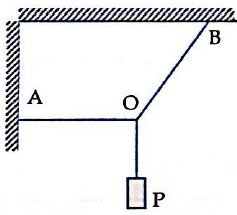
\includegraphics[scale=0.8]{../figs/VN11-Y21-PH-SYL-005-6.jpg}
		\end{center}
		\begin{mcq}(2)
			\item $30\sqrt{2}\ \text{N}$ và $60\sqrt{2}\ \text{N}$.
			\item $60\ \text{N}$ và $60\sqrt{2}\ \text{N}$.
			\item $30\sqrt{2}\ \text{N}$ và $120\ \text{N}$.
			\item $45\ \text{N}$ và $60\sqrt{2}\ \text{N}$.
		\end{mcq}
	}
	\loigiai{\textbf{Đáp án: B.}
		
		\begin{center}
			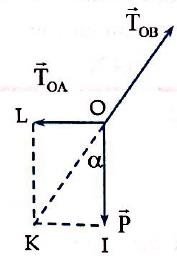
\includegraphics[scale=0.8]{../figs/VN11-Y21-PH-SYL-005-7.jpg}
		\end{center}
		
		Các lực tác dụng vào điểm treo O như hình vẽ.
		
		Góc $\alpha$ là góc giữa OP và OB, $\alpha=45^\circ$.
		$$\text{OI}=\text{OK}\cdot \cos \alpha\Rightarrow \text{OK}=\dfrac{\text{OI}}{\cos \alpha}\Rightarrow T_\text{OB}=\dfrac{P}{\cos \alpha}=60\sqrt{2}\ \text{N} $$
		
		Tương tự:   $$T_\text{OA}=T_\text{OB}\cdot \sin 45^\circ=60\ \text{N}$$
		
		
	}
	
	\item \mkstar{4}
	
	\cauhoi{ Một quả cầu đồng chất có khối lượng $\SI{4}{\kilogram}$ được treo vào tường thẳng đứng nhờ một sợi dây hợp với tường một góc $\alpha=30^\circ$. Bỏ qua ma sát ở chỗ tiếp xúc của quả cầu với tường. Lấy $g=\SI{9,8}{\meter/\second^2}$. Lực của tường tác dụng lên quả cầu có độ lớn
		\begin{center}
			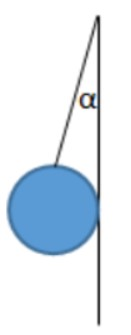
\includegraphics[scale=0.8]{../figs/10-3-1.jpg}
		\end{center}
		\begin{mcq}(4)
			\item $\SI{23}{\newton}$.
			\item $\SI{22,6}{\newton}$.
			\item $\SI{20}{\newton}$.
			\item $\SI{19,6}{\newton}$.
		\end{mcq}
	}
	\loigiai{\textbf{Đáp án: B.}
		
		Các lực tác dụng lên quả cầu được biểu diễn như hình vẽ:
		\begin{center}
			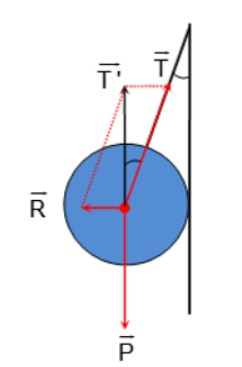
\includegraphics[scale=0.7]{../figs/10-3-2.jpg}
		\end{center}
		Điều kiện cân bằng của quả cầu là:
		$$\vec{R}+\vec{T}=\vec{T}'=-\vec{P}.$$
		Ta có:
		$$\tan\alpha=\dfrac{R}{P}\Rightarrow R=P\cdot \tan\alpha=\SI{22,6}{\newton}.$$
		
		
		
	}
	\item \mkstar{4}
	
	\cauhoi{ Một thanh đồng chất nằm cân bằng ở tư thế nằm ngang bởi hai sợi dây buộc vào hai đầu của nó như hình vẽ. Lực căng dây có độ lớn $T_1=T_2=\SI{10}{\newton}$, góc $\theta=37^\circ$. Trọng lượng của thanh bằng
		\begin{center}
			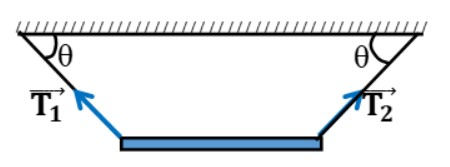
\includegraphics[scale=0.7]{../figs/10-3-3.jpg}
		\end{center}
		\begin{mcq}(4)
			\item $\SI{10}{\newton}$.
			\item $\SI{20}{\newton}$.
			\item $\SI{12}{\newton}$.
			\item $\SI{16}{\newton}$.
		\end{mcq}
		
		
	}
	\loigiai{\textbf{Đáp án: C.}
		
		Trọng lượng của thanh bằng
		$$P=mg=2T\sin\theta=\SI{12}{\newton}.$$
		
		
		
	}
\end{enumerate}

\whiteBGstarEnd

\loigiai{\begin{center}
		\textbf{BẢNG ĐÁP ÁN}
	\end{center}
	\begin{center}
		\begin{tabular}{|m{2.8em}|m{2.8em}|m{2.8em}|m{2.8em}|m{2.8em}|m{2.8em}|m{2.8em}|m{2.8em}|m{2.8em}|m{2.8em}|}
			\hline
			1.C  & 2.B  & 3. B & 4.B  & 5.D  & 6.D  & 7.B  & 8.B  & 9.B  & 10.A  \\
			\hline
			11.A  & 12.C  & 13.A  & 14.A  & 15.B  & 16.D  & 17.A  & 18.B  & 19.B  & 20.C  \\
			\hline
			
		\end{tabular}
\end{center}}
\chapter{Pre-course: Ba định luật Newton}
\whiteBGstarBegin

\begin{enumerate}[label=\bfseries Câu \arabic*:]
	
	\item \mkstar{1}
	
	\cauhoi
	{Định luật I Niu-tơn xác nhận rằng
		\begin{mcq}
			\item do quán tính nên mọi vật đang chuyển động đều có xu hướng dừng lại.
			\item với mỗi lực tác dụng đều có một phản lực trực đối.
			\item vật giữ nguyên trạng thái đứng yên hoặc chuyển động thẳng đều khi nó không chịu tác dụng của bất kì lực nào.
			\item khi hợp lực tác dụng lên vật bằng 0 thì vật không thể chuyển động được.
		\end{mcq}
	}
	
	\loigiai
	{\textbf{Đáp án: C.}
		
		Định luật I - Niu-tơn: Nếu một vật không chịu tác dụng của lực nào hoặc chịu tác dụng của các lực có hợp lực bằng không, thì nó giữ nguyên trạng thái đứng yên hoặc chuyển động thẳng đều.
		
		
	}
	\item \mkstar{1}
	
	\cauhoi
	{Hai lực trực đối cân bằng là hai lực
		\begin{mcq}
			\item tác dụng vào cùng một vật.
			\item không bằng nhau về độ lớn.
			\item bằng nhau về độ lớn nhưng không nhất thiết phải cùng giá.
			\item có cùng độ lớn, cùng phương, ngược chiều, tác dụng vào hai vật khác nhau.
		\end{mcq}
	}
	\loigiai
	{\textbf{Đáp án: D.}
		
		Hai lực trực đối cân bằng là hai lực có cùng độ lớn, cùng phương, ngược chiều, tác dụng vào hai vật khác nhau.
		
		
	}
	\item \mkstar{1}
	
	\cauhoi
	{Kết luận nào sau đây đúng?
		\begin{mcq}
			\item Nếu không có lực tác dụng vào vật thì vật không thể chuyển động được.
			\item Không cần có lực tác dụng vào vật thì vật vẫn có thể chuyển động tròn đều được.
			\item Lực là nguyên nhân duy trì chuyển động của một vật.
			\item Lực là nguyên nhân làm biến đổi chuyển động của một vật.
		\end{mcq}
	}
	
	\loigiai
	{\textbf{Đáp án: D.}
		
		Lực là nguyên nhân làm biến đổi chuyển động của một vật.
		
		
	}
	\item \mkstar{2}
	
	\cauhoi
	{Trường hợp nào sau đây có liên quan đến quán tính?
		\begin{mcq}(2)
			\item Vật rơi tự do.
			\item Vật rơi trong không khí.
			\item Chiếc bè trôi trên sông.
			\item Giũ quần áo cho sạch bụi.
		\end{mcq}
	}
	
	\loigiai
	{\textbf{Đáp án: D.}	
		
		Quán tính là tính chất của mọi vật có xu hướng bảo toàn vận tốc cả về hướng và độ lớn.
		
		
	}
	\item \mkstar{2}
	
	\cauhoi
	{Vật nào sau đây chuyển động theo quán tính?
		\begin{mcq}
			\item Vật chuyển động tròn đều.
			\item Vật chuyển động trên quỹ đạo thẳng.
			\item Vật chuyển động thẳng đều.
			\item Vật chuyển động khi tất cả các lực tác dụng lên vật mất đi.
		\end{mcq}
	}
	
	\loigiai
	{\textbf{Đáp án: D.}
		
	Chuyển động theo quán tính là chuyển động khi tất cả các lực tác dụng lên vật mất đi.
		
		
	}
	\item \mkstar{2}
	
	\cauhoi
	{Người ta dùng búa đóng một cây đinh vào một khối gỗ.
		\begin{mcq}
			\item Lực do đinh tác dụng vào búa lớn hơn lực do búa tác dụng vào đinh.
			\item Lực do đinh tác dụng vào búa nhỏ hơn lực do búa tác dụng vào đinh.
			\item Lực do đinh tác dụng vào búa bằng lực do búa tác dụng vào đinh.
			\item Lực do đinh tác dụng vào búa có thể lớn hơn hoặc nhỏ hơn lực do búa tác dụng vào đinh.
		\end{mcq}
	}
	
	\loigiai
	{\textbf{Đáp án: C.}
		
		Cặp lực trực đối trong định luật III Niu-tơn bằng nhau về độ lớn.
		
		
	}
	\item \mkstar{2}
	
	\cauhoi
	{Các lực tác dụng vào vật cân bằng nhau khi vật
		\begin{mcq}(2)
			\item chuyển động thẳng đều.
			\item chuyển động thẳng biến đổi đều.
			\item chuyển động thẳng.
			\item chuyện động tròn đều
		\end{mcq}
	}
	
	\loigiai
	{\textbf{Đáp án: A.}
		
		Các lực tác dụng vào vật cân bằng nhau khi vật chuyển động không có gia tốc ($\vec a = 0$), bao gồm chuyển động thẳng đều.
		
		
	}
	\item \mkstar{2}
	
	\cauhoi
	{Một vật đang chuyển động với vận tốc $3\ \text{m/s}$. Nếu bỗng nhiên các lực tác dụng lên nó mất đi thì
		\begin{mcq}
			\item vật dừng lại ngay.
			\item vật đổi hướng chuyển động.
			\item vật chuyển động chậm dần rồi mới dừng lại.
			\item vật tiếp tục chuyển động như cũ.
		\end{mcq}
	}
	
	\loigiai
	{\textbf{Đáp án: D.}
		
		Định luật I - Niu-tơn: Nếu một vật không chịu tác dụng của lực nào hoặc chịu tác dụng của các lực có hợp lực bằng không, thì nó giữ nguyên trạng thái đứng yên hoặc chuyển động thẳng đều.
		
		
	}
	\item \mkstar{2}
	
	\cauhoi
	{Kết luận nào sau đây đúng?
		\begin{mcq}
			\item Khi vật không chịu tác dụng của lực nào thì vật phải đứng yên.
			\item Một vật có thể chịu tác dụng đồng thời của nhiều lực mà vẫn đứng yên.
			\item Một vật không thể chuyển động được nếu không có lực nào tác dụng vào nó.
			\item Các vật luôn chuyển động theo phương của lực tác dung.
		\end{mcq}
	}
	
	\loigiai
	{\textbf{Đáp án: B.}
		
		Một vật có thể chịu tác dụng của đồng thời nhiều lực (cân bằng) mà vẫn đứng yên. Một vật không chịu tác dụng của lực nào thì vẫn có thể chuyển động thẳng đều theo quán tính.
		
		
	}
	\item \mkstar{2}
	
	\cauhoi
	{Hai xe A ($m_\text A$) và xe B ($m_\text B$) đang chuyển động với cùng một vận tốc thì tắt máy và chịu cùng lực tác dụng của một lực hãm $F$ như nhau. Sau khi chịu lực hãm, xe A còn đi thêm một đoạn $s_\text A$, xe B còn đi thêm một đoạn $s_\text B$ nữa cho đến khi dừng hẳn. Biết $s_\text B < s_\text A$, điều nào sau đây là đúng khi so sánh khối lượng của hai xe?
		\begin{mcq}(2)
			\item $m_\text A > m_\text B$.
			\item $m_\text A < m_\text B$.
			\item $m_\text A = m_\text B$
			\item Chưa đủ điều kiện để kết luận.
		\end{mcq}
	}
	
	\loigiai
	{\textbf{Đáp án: A.}
		
		Khối lượng đặc trưng cho mức quán tính của một vật, vật có khối lượng lớn hơn thì có xu hướng giữ nguyên vận tốc lớn hơn. Vậy khi $s_\text B < s_\text A$ thì $m_\text A > m_\text B$.
		
		
	}
	\item \mkstar{2}
	
	\cauhoi
	{Trong trường hợp nào dưới đây, vật chuyển động theo hướng của hợp lực tác dụng vào vật?
		\begin{mcq}
			\item Vật chuyển động thẳng đều.
			\item Vật chuyển động thẳng nhanh dần đều.
			\item Vật chuyển động thẳng chậm dần đều.
			\item Vật chuyển động tròn đều.
		\end{mcq}
	}
	
	\loigiai
	{\textbf{Đáp án: B.}
		
		Khi vật chuyển động thẳng nhanh dần đều thì $\vec a$ cùng phương, cùng chiều với $\vec v$. Do đó $\vec v$ cùng phương, cùng chiều với $\vec F$.
		
		
	}
	\item \mkstar{3}
	
	\cauhoi
	{Một lực có độ lớn $\SI{2}{\newton}$ tác dụng vào một vật có khối lượng $\SI{1}{\kilogram}$ lúc đầu đứng yên. Quãng đường mà vật đi được trong khoảng thời gian $\SI{2}{\second}$ là
		\begin{mcq}(4)
			\item $\SI{4}{\meter}$.
			\item $\SI{1}{\meter}$.
			\item $\SI{0,5}{\meter}$.
			\item $\SI{2}{\meter}$.
		\end{mcq}
	}
	
	\loigiai
	{\textbf{Đáp án: A.}
		
		Áp dụng công thức $a=\dfrac{F}{m}$ và $s=v_0t+\dfrac{at^2}{2}$.
		
		Suy ra $s=\SI{4}{\meter}$.
		
		
	}
	\item \mkstar{3}
	
	\cauhoi
	{Một vật đang đứng yên, được truyền một lực $F$ thì vận tốc tăng thêm $\SI{2}{\meter / \second}$ sau $\SI{5}{\second}$. Nếu giữ nguyên hướng của lực mà tăng độ lớn lên gấp 2 thì vận tốc của vật sau $\SI{8}{\second}$ sẽ tăng thêm bao nhiêu?
		\begin{mcq}(4)
			\item $\SI{4}{\meter / \second}$.
			\item $\SI{6.4}{\meter / \second}$.
			\item $\SI{3.2}{\meter / \second}$.
			\item $\SI{2}{\meter / \second}$.
		\end{mcq}
	}
	
	\loigiai
	{\textbf{Đáp án: B.}
		
		Gia tốc của vật dưới tác dụng của lực $F$: $a=\dfrac{\Delta v}{\Delta t}=\SI{0.4}{\meter / \second \squared}$.
		
		Gia tốc của vật dưới tác dụng của lực $2F$: $a'=\dfrac{2F}{m}=2a=\SI{0.8}{\meter / \second \squared}$.
		
		Vận tốc của vật sau tăng thêm sau $\SI{8}{\second}$: $\Delta v= a' \Delta t'=\SI{6.4}{\meter / \second}$.
		
		
	}
	\item \mkstar{3}
	
	\cauhoi
	{Một quả bóng khối lượng $\SI{200}{\gram}$ bay với vận tốc $\SI{90}{\kilo\meter/\hour}$ đến đập vuông góc vào tường rồi bật trở lại theo phương cũ với vận tốc $\SI{54}{\kilo\meter/\hour}$. Thời gian va chạm giữa bóng và tường là $\SI{0,05}{\second}$. Độ lớn lực của tường tác dụng lên quả bóng là
		\begin{mcq}(4)
			\item $\SI{160}{\newton}$.
			\item $\SI{200}{\newton}$.
			\item $\SI{210}{\newton}$.
			\item $\SI{120}{\newton}$.
		\end{mcq}
	}
	
	\loigiai
	{\textbf{Đáp án: A.}
		
		Chọn chiều dương cùng chiều bật ra của quả bóng.
		
		Áp dụng định luật II và III Newton:
		$$F_\text{tường}=F_\text{bóng}=ma=m\dfrac {v-v_0}{\Delta t}=\SI{0,2}{\kilogram}\cdot\dfrac{\SI{15}{\meter/\second}-(\SI{-25}{\meter/\second})}{\SI{0,05}{\second}}=\SI{160}{\newton}.$$
		
		
	}
	\item \mkstar{3}
	
	\cauhoi
	{Một ô tô có khối lượng 1 tấn đang chuyển động với $v=54\ \text{km/h}$ thì tắt máy, hãm phanh, chuyển động chậm dần đều. Biết độ lớn lực hãm $3000\ \text N$. Xác định quãng đường xe đi được cho đến khi dừng lại.
		\begin{mcq}(4)
			\item $32,5\ \text m$.
			\item $37,5\ \text m$.
			\item $42,5\ \text m$.
			\item $47,5\ \text m$.
		\end{mcq}
	}
	
	\loigiai
	{\textbf{Đáp án: B.}
		
		Chọn chiều dương là chiều chuyển động, gốc thời gian lúc bắt đầu hãm phanh.
		
		Áp dụng định luật II Newton:
		\[ \vec a = \dfrac {\vec F}{m} \Rightarrow a=\dfrac{F}{m} = \dfrac{-3000}{1000} = -3\ \text{m/s}^2\]
		
		Mà $v^2 - v_0 ^2 = 2as$, suy ra $s=37,5\ \text m$.
		
		
	}
	\item \mkstar{3}
	
	\cauhoi
	{Một người đang đi xe đạp với vận tốc $V_0$ thì ngừng đạp và hãm phanh. Xe đi tiếp được $40\ \text m$ thì dừng lại. Lực hãm và lực ma sát có tổng độ lớn $14\ \text N$. Khối lượng cả người và xe là $70\ \text {kg}$. Tính $V_0$.
		\begin{mcq}(4)
			\item $V_0 = 2\ \text{m/s}$.
			\item $V_0= 3\ \text{m/s}$.
			\item $V_0= 4\ \text{m/s}$.
			\item $V_0=5\ \text{m/s}$.
		\end{mcq}
	}
	
	\loigiai
	{\textbf{Đáp án: C.}	
		
		Gia tốc của xe:
		\[a=\dfrac{F}{m}=\dfrac{-14}{70} = -0,2\ \text{m/s}^2\]
		
		Mà $0-V_0^2 = 2as \Rightarrow V_0 = 4\ \text{m/s}$
		
		
	}
	\item \mkstar{3}
	
	\cauhoi
	{Một xe tải khối lượng 1 tấn, sau khi khởi hành được $10\ \text s$ đạt vận tốc $18\ \text{km/h}$. Biết lực cản mà mặt đường tác dụng lên xe là $500\ \text N$. Tính lực phát động của động cơ.
		\begin{mcq}(4)
			\item $500\ \text N$.
			\item $750\ \text N$.
			\item $1000\ \text N$.
			\item $1500\ \text N$.
		\end{mcq}
	}
	
	\loigiai
	{\textbf{Đáp án: C.}
		
		Gia tốc của xe:
		\[a = \dfrac{v-v_0}{\Delta t} = \dfrac{1}{2}\ \text{m/s}^2\]
		
		Mà $F-F_\text c = ma \Rightarrow F = F_\text c + ma = 500 + 500 = 1000\ \text N$
		
		
	}
	\item \mkstar{4}
	
	\cauhoi
	{Một viên bi A có khối lượng $\SI{300}{\gram}$ đang chuyển động với vận tốc $\SI{3}{\meter / \second}$ thì va chạm vào viên bi B có khối lượng $\SI{600}{\gram}$ đang đứng yên trên mặt bàn nhẵn nằm ngang. Biết thời gian diễn ra va chạm là $\SI{0.2}{\second}$. Sau va chạm, viên bi B chuyển động với vận tốc $\SI{0.5}{\meter}$ cùng chiều chuyển động ban đầu của bi A. Tốc độ chuyển động của bi A sau va chạm là
		\begin{mcq}(4)
			\item $\SI{1}{\meter / \second}$.
			\item $\SI{3}{\meter / \second}$.
			\item $\SI{4}{\meter / \second}$.
			\item $\SI{2}{\meter / \second}$.
		\end{mcq}
	}
	
	\loigiai
	{\textbf{Đáp án: C.}
		
		Ta xét chuyển động của viên bi B: Trước va chạm có vận tốc $v_\text B = \SI{0}{\meter / \second}$, sau va chạm có vận tốc $v_\text B'=\SI{0.5}{\meter/ \second}$. Suy ra $a_\text B=\dfrac{v_\text B'-v_\text B}{\Delta t}=\SI{2.5}{\meter / \second \squared}$.
		
		Áp dụng định luật II và III Niu-tơn:
		$|F_\text {AB}| = |F_\text {BA}| \Leftrightarrow m_\text A a_\text A = m_\text B a_\text B \Rightarrow a_\text A = \SI{5}{\meter / \second \squared}$.
		
		Vận tốc của bi A sau va chạm: $a_\text A = \dfrac{v_\text A'-v_\text A}{\Delta t}\Rightarrow v_\text A' = \SI{4}{\meter / \second}$.
		
		
	}
	\item \mkstar{4}
	
	\cauhoi
	{Cho cơ hệ như hình vẽ. Vật A có khối lượng $m_1=200\ \text g$, vật B có khối lượng $m_2=120\ \text g$ nối với nhau bởi một sợi dây nhẹ, không dãn. Hệ số ma sát trượt giữa hai vật và mặt phẳng ngang là $\mu = 0,4$. Tác dụng vào A một lực kéo $\vec F$ theo phương ngang. Biết rằng dây nối hai vật chỉ chịu được lực căng tối đa $T_0=0,6\ \text N$. Lấy $g=10\ \text{m/s}^2$. Tìm lực $F$ lớn nhất để dây không bị đứt.
		\begin{center}
			\includegraphics[scale=0.8]{../figs/VN11-Y21-PH-SYL-007-1}
		\end{center}
		\begin{mcq}(4)
			\item $0,96\ \text N$.
			\item $0,375\ \text N$.
			\item $1,5\ \text N$.
			\item $1,6\ \text N$.
		\end{mcq}
	}
	
	\loigiai
	{\textbf{Đáp án: D.}
		
		\begin{center}
			\includegraphics[scale=0.8]{../figs/VN11-Y21-PH-SYL-007-2}
		\end{center}
		
		Áp dụng định luật II Niu-tơn cho hệ vật:
		\[F-\mu (m_1 + m_2)g=(m_1+m_2)a \Rightarrow a = \dfrac{F}{m_1 + m_2} - \mu g\]
		
		Áp dụng định luật II Niu-tơn cho vật B:
		\[T-\mu m_2g=m_2 a \Rightarrow T = (\mu g + a)m_2 = \dfrac{F m_2}{m_1 + m_2} \Rightarrow F = \dfrac{m_1 + m_2}{m_2}T\]
		
		Do dây chỉ chịu được lực căng tối đa $0,6\ \text N$, nên thay số ta tính được $F$ tối đa là $F=1,6\ \text N$.
		
		
	}
	\item \mkstar{4}
	
	\cauhoi
	{Cho cơ hệ như hình vẽ. Mặt phẳng nghiêng cố định, nghiêng góc $\alpha$ so với phương ngang. Hai chất điểm khối lượng $m_1$, $m_2$ được nối với nhau bởi dây nhẹ, không dãn vắt qua ròng rọc nhẹ có kích thước không đáng kể. Biết rằng $m_2 > m_1 \sin \alpha$. Bỏ qua mọi ma sát, cho gia tốc trọng trường là $g$. Thả hai vật chuyển động tự do, tìm gia tốc của mỗi vật.
		\begin{center}
			\includegraphics[scale=0.8]{../figs/VN11-Y21-PH-SYL-007-3}
		\end{center}
		
		\begin{mcq}(2)
			\item $a_1=a_2 = \dfrac{m_2 - m_1 \sin \alpha}{m_1 + m_2}g$.
			\item $a_1=a_2 = \dfrac{m_2 - m_1 \sin \alpha}{m_1 - m_2}g$.
			\item $a_1=a_2 = \dfrac{m_2 + m_1 \sin \alpha}{m_1 + m_2}g$.
			\item $a_1=a_2 = \dfrac{(m_2 - m_1) \sin \alpha}{m_1 + m_2}g$.
		\end{mcq}
	}
	
	\loigiai
	{\textbf{Đáp án: A.}
		
		\begin{center}
			\includegraphics[scale=0.8]{../figs/VN11-Y21-PH-SYL-007-4}
		\end{center}
		
		Do $m_2 > m_1 \sin \alpha$ nên $m_2$ sẽ đi xuống.
		
		Áp dụng định luật II Niu-tơn cho mỗi vật:
		\begin{align*}
			\vec T_1 + \vec N + \vec P_1 &= m_1 \vec a_1 \\
			\vec T_2 + \vec P_2 &= m_2 \vec a_2
		\end{align*}
		
		Do dây nhẹ, không dãn, ròng rọc không khối lượng nên $T_1 = T_2 = T$, $a_1 = a_2 = a$.
		
		Chiếu các vectơ lên phương chuyển động của mỗi vật, ta được:
		\begin{align*}
			T - P_1 \sin \alpha &= m_1 a \\
			-T + P_2 &= m_2 a
		\end{align*}
		
		Suy ra $a=\dfrac{m_2 - m_1 \sin \alpha}{m_1 + m_2}g$.
		
		
	}
\end{enumerate}

\whiteBGstarEnd

\loigiai{\begin{center}
		\textbf{BẢNG ĐÁP ÁN}
	\end{center}
	\begin{center}
		\begin{tabular}{|m{2.8em}|m{2.8em}|m{2.8em}|m{2.8em}|m{2.8em}|m{2.8em}|m{2.8em}|m{2.8em}|m{2.8em}|m{2.8em}|}
			\hline
			1. C & 2. D & 3. D & 4. D & 5. D & 6. C & 7. A & 8. D & 9. B & 10. A \\
			\hline
			11. B & 12. A & 13. B & 14. A & 15. B & 16. C & 17. C & 18. C & 19. D & 20. A \\
			\hline
			
		\end{tabular}
\end{center}}
\end{document}